\documentclass{article}
\usepackage{graphicx}
\usepackage{amssymb}
\usepackage{amsmath}
\usepackage[dvipsnames]{xcolor} 
\usepackage{mdframed}
\usepackage{algorithm} 
\usepackage{algpseudocode}
\usepackage{xfrac}
\usepackage{wrapfig}
\usepackage{lipsum}
\usepackage{IEEEtrantools}
\usepackage{empheq}
\usepackage{calc}

\algtext*{EndFor}
\algtext*{EndIf}

\usepackage[style=numeric, sorting=none]{biblatex} 
\addbibresource{refs.bib}

\usepackage{hyperref}
\hypersetup{
    colorlinks=true,
    linkcolor=blue,
    filecolor=magenta,
    urlcolor=cyan,
    citecolor=blue,
    linktoc=all,            % make both text AND page number in TOC into links
    linkbordercolor=black,  % unused when colorlinks=true
}

\newmdenv[
  backgroundcolor=gray!10,
  linecolor=gray!40,
  linewidth=0.8pt,
  roundcorner=4pt,
  innertopmargin=10pt,
  innerbottommargin=10pt,
  innerleftmargin=12pt,
  innerrightmargin=12pt,
  skipabove=8pt,
  skipbelow=8pt
]{derivation}

\newmdenv[
  backgroundcolor=gray!10,
  linecolor=gray!40,
  linewidth=0.8pt,
  roundcorner=4pt,
  innertopmargin=10pt,
  innerbottommargin=10pt,
  innerleftmargin=12pt,
  innerrightmargin=12pt,
  skipabove=8pt,
  skipbelow=8pt,
  frametitlefont=\bfseries,
  frametitleaboveskip=8pt,
  frametitlebelowskip=0pt,
]{definitionbox}

\newmdenv[
  backgroundcolor=gray!20,
  linecolor=gray!80,
  linewidth=0.8pt,
  roundcorner=4pt,
  innertopmargin=10pt,
  innerbottommargin=10pt,
  innerleftmargin=12pt,
  innerrightmargin=12pt,
  skipabove=8pt,
  skipbelow=8pt,
  frametitlefont=\bfseries,
  frametitleaboveskip=8pt,
  frametitlebelowskip=0pt,
]{reminder}

\newcommand{\doubleline}{
    \vspace{1ex}
    \hrule
    \pagebreak[1] % Encourages not breaking the page between lines
    \vspace{0.4ex}
    \hrule
    \vspace{1ex}
}

\newcommand{\der}[2]{\dfrac{d\, #1}{d\, #2}}
\newcommand{\pd}[2]{\dfrac{\partial\, #1}{\partial\, #2}}
\newcommand{\pdc}[2]{\frac{\partial #1}{\partial #2}}
\newcommand{\pdv}[2]{\dfrac{\partial^2\, #1}{\partial\, #2^2}}
\newcommand{\pdm}[3]{\dfrac{\partial^2\, #1}{\partial\, #2 \partial\, #3}}
\newcommand{\drop}[1]{\textcolor{red}{#1}}
\newcommand{\maybedrop}[1]{\textcolor{orange}{#1}}
\newcommand{\invd}[1]{\tilde{d}_{#1}}

\definecolor{MyGreen}{RGB}{0, 158, 0}
\newcommand{\red}[1]{\textcolor{red}{#1}}
\newcommand{\blue}[1]{\textcolor{blue}{#1}}
\newcommand{\green}[1]{\textcolor{MyGreen}{#1}}

\newcommand{\graycomment}[1]{\Comment{\textcolor{gray}{#1}}}

\title{Inverse Physics Notes}
\author{Umberto Castellani, Matteo Boroni Grazioli}

\begin{document}

\begin{titlepage}
    \centering

    % --- Institution ---
    
\includegraphics[width=0.45\textwidth]{images/univr_logo.png}\par
    \vspace{0.5cm}
    {\scshape\large Università degli Studi di Verona\par}
    {\scshape Dipartimento di Informatica\par}
    \vspace{1.5cm}

    % --- Document type ---
    {\large\bfseries Technical Report\par}
    \vspace{1.5cm}

    % --- Title ---
    \rule{\linewidth}{0.4pt}\par
    \vspace{0.6cm}
    {\huge\bfseries Differentiable Physics Simulation:\\[0.3cm]
     Methods for Cloth and Inverse Problems\par}
    \vspace{0.6cm}
    \rule{\linewidth}{0.4pt}\par
    \vspace{2cm}

    % --- Authors ---
    {\large
     Umberto Castellani \\[0.2cm]
     Matteo Boroni Grazioli\par}
    \vspace{0.4cm}
    % {\small \texttt{name.surname@univr.it}\par}  % adjust to real addresses

    \vfill
    
    {\large June 2026\par}

\end{titlepage}

\thispagestyle{empty}

\newpage

\

\newpage

\pagenumbering{roman}
\begingroup
  \hypersetup{linkcolor=black}
  \tableofcontents
\endgroup
\newpage

\pagenumbering{arabic}

\begin{abstract}
Physically based simulation of deformable bodies offers a spectrum of methods, each trading off physical accuracy against speed and stability. This report surveys these methods with a focus on cloth and thin shells, a class of deformable body whose high contact area and frequent self-collisions make accurate collision handling particularly challenging in interactive settings. Our broader motivation is the \emph{inverse} problem: recovering internal cloth material parameters from real-world 3D-captured dynamics of garments in motion. This goal shapes the survey in two ways.

First, since the recovered parameters are intended for use in interactive environments, we concentrate primarily on methods capable of real-time forward simulation, examining XPBD \cite{macklin2016xpbd} and Projective Dynamics \cite{bouaziz2023projective} in depth, while also considering computationally heavier but more accurate approaches such as Incremental Potential Contact \cite{Li2020IPC}. Second, solving inverse problems by gradient-based optimization requires the simulator to be \emph{differentiable}, that is, able to compute gradients of an objective with respect to chosen parameters by backpropagating through the timestep integrator. For several of these simulation methods we therefore derive the corresponding gradient computation, relying on analytical gradients of the update formulas, the adjoint method, and implicit differentiation.

A recurring difficulty is the differentiation of collision response, which is inherently discontinuous. We analyze several collision-handling strategies and whether each can be differentiated, including post-projection corrections, penalty forces and constraints \cite{macklin2020primal}, a constrained quadratic-program formulation \cite{liang2019differentiable}, and smooth barrier potentials \cite{Li2020IPC}. The goal is to map the trade-offs between physical fidelity, interactive performance, and differentiability.
\end{abstract}

\newpage

\section*{Introduction}

\paragraph{Chapter~\ref{sec:math} — Math Background.}
Collects the general mathematical tools used throughout the report, independent of any specific physical model or algorithm.

\paragraph{Chapter~\ref{sec:implict_sim} — Implicit Simulator.}
Introduces implicit (BDF1) time integration for particle systems and shows how the resulting nonlinear equations of motion are discretized. It then presents two practical solution strategies: a single-linearization solve and the full multi-iteration Newton--Raphson scheme.

\paragraph{Chapter~\ref{sec:adjoint} — Gradient Computation via Adjoint Method.}
Derives the adjoint method from first principles as a means of computing gradients of an objective with respect to a simulator's parameters. The method is then specialized to explicit time-stepping functions.

\paragraph{Chapter~\ref{sec:baraff_witkin} — Baraff--Witkin Cloth Simulation Model.}
Describes the constraint-based formulation of the Baraff--Witkin cloth model and its associated elastic energies. All components needed for a single-linear solve, namely the energy Jacobians and Hessians, are derived for the three cloth constraints: stretch, shear, and dihedral bending.

\paragraph{Chapter~\ref{sec:descent_methods} — Descent Methods.}
Provides a general overview of descent-based formulations of implicit time integration for deformable bodies. It recasts several existing simulation methods within a unified descent framework.

\paragraph{Chapter~\ref{sec:primal_dual} — Primal/Dual Descent Methods.}
Explains the distinction between primal and dual descent formulations of implicit Euler integration, deriving the objective, algorithm, and Newton update for each. It also presents a collision and friction handling scheme tailored to these descent methods.

\paragraph{Chapter~\ref{sec:xpbd} — XPBD.}
Describes and derives the XPBD simulation method starting from the dual objective of the previous chapter. It then develops the differentiable version of the algorithm for both single- and multi-iteration solves, focusing on gradients with respect to the constraint compliance parameters.

\paragraph{Chapter~\ref{sec:collisions} — Collisions.}
Surveys strategies a cloth simulator can use to handle collisions and friction, operating at both the vertex level and the primitive level. For each approach it covers detection, response, and the corresponding derivatives required for gradient computation.

\paragraph{Chapter~\ref{sec:implicit_diff} — Implicit Differentiation.}
Presents the mathematics of implicit differentiation as a general framework for backpropagating. The framework is then specialized to different problems: a linear solve, a QP with linear inequality constraints, a generic constrained QP, and a linear complementarity problem.

\paragraph{Chapter~\ref{sec:DiffCloth} — Differentiable Cloth Simulation for Inverse Problems.}
Describes the forward and backward simulation pipeline adapted from \cite{liang2019differentiable}.

\paragraph{Chapter~\ref{sec:pd} — Projective Dynamics (PD).}
Describes and derives the Projective Dynamics method, with strain constraints specialized to cloth. It then covers its extension to dry frictional contact and the differentiable counterparts of both the base method and the contact formulation for gradient computation.

\paragraph{Chapter~\ref{sec:ipc} — Incremental Potential Contact (IPC).}
Provides an in-depth description of the IPC method, including its smooth contact barrier energy and collision culling. It details the computation of energy Jacobians and SPD-projected Hessians, with the Stable Neo-Hookean model worked out in full.

\newpage



\section{Math Background}
\label{sec:math}

\subsection{Newton-Raphson for Root-Finding}
\label{sec:newton_raphson}

Given a smooth function $\mathbf{f} : \mathbb{R}^n \to \mathbb{R}^n$, we seek $\mathbf{x}^* \in \mathbb{R}^n$ such that $\mathbf{f}(\mathbf{x}^*) = \mathbf{0}$. Starting from an initial guess $\mathbf{x}^{(0)}$, Newton-Raphson iteratively refines the estimate by linearizing $\mathbf{f}$ around the current iterate. At iteration $k$, the first-order Taylor expansion gives:
%
\begin{equation}
    \mathbf{f}(\mathbf{x}^{(k)} + \delta \mathbf{x}) \approx \mathbf{f}(\mathbf{x}^{(k)}) + \pd{\mathbf{f}}{\mathbf{x}}\bigg|_{\mathbf{x}^{(k)}} \delta \mathbf{x}
\end{equation}
%
Setting this to zero and solving for the correction $\delta \mathbf{x}$ yields the linear system:
%
\begin{equation}
    \pd{\mathbf{f}}{\mathbf{x}}\bigg|_{\mathbf{x}^{(k)}} \delta \mathbf{x} = -\mathbf{f}(\mathbf{x}^{(k)})
\end{equation}
%
The iterate is then updated as $\mathbf{x}^{(k+1)} = \mathbf{x}^{(k)} + \delta \mathbf{x}$. The process repeats until $\|\mathbf{f}(\mathbf{x}^{(k)})\| < \epsilon$.

\begin{algorithm}[H]
\caption{Newton-Raphson Root-Finding}
\label{alg:newton_raphson}
\begin{algorithmic}[1]
\addtolength{\itemsep}{0.5ex}
\Function{NewtonRaphson}
{$\mathbf{f},\, \mathbf{x}^{(0)},\, \epsilon,\, N$}
    \State $\mathbf{x} \gets \mathbf{x}^{(0)}$
    \For{$k = 0, 1, \ldots, N$}
        \State $\mathbf{r} \gets \mathbf{f}(\mathbf{x})$
        \If{$\|\mathbf{r}\| < \epsilon$}
            \State \Return $\mathbf{x}$
        \EndIf
        \State $\mathbf{A} \gets \pdc{\mathbf{f}}{\mathbf{x}}\big|_{\mathbf{x}}$
        \State $\textsc{Solve}\;\; \mathbf{A}\, \delta\mathbf{x} = -\mathbf{r}$
        \State $\mathbf{x} \gets \mathbf{x} + \delta\mathbf{x}$
    \EndFor
    \State \Return $\mathbf{x}$
\EndFunction
\end{algorithmic}
\end{algorithm}

\subsection{Finite Difference Approximations}
\label{sec:finite-difference}

Let $f(t)$ denote a scalar function of $t \in \mathbb{R}$, and let
$\Delta t \in \mathbb{R}_{>0}$ denote a fixed step size. The objective is
to approximate the derivative $\frac{\mathrm{d}f}{\mathrm{d}t}$ at a point $t$
using evaluations of $f$ at neighboring points, without requiring an
analytical expression for the derivative.
\newline The governing relations are the forward and backward Taylor expansions
of $f$ about $t$,
\begin{align}
f(t+\Delta t) &= f(t) + \frac{\mathrm{d}f}{\mathrm{d}t}(t)\,\Delta t
  + \frac{\mathrm{d}^2 f}{\mathrm{d}t^2}(t)\,\frac{\Delta t^2}{2!}
  + \frac{\mathrm{d}^3 f}{\mathrm{d}t^3}(t)\,\frac{\Delta t^3}{3!}
  + O(\Delta t^4) \label{eq:taylor-fwd} \\
f(t-\Delta t) &= f(t) - \frac{\mathrm{d}f}{\mathrm{d}t}(t)\,\Delta t
  + \frac{\mathrm{d}^2 f}{\mathrm{d}t^2}(t)\,\frac{\Delta t^2}{2!}
  - \frac{\mathrm{d}^3 f}{\mathrm{d}t^3}(t)\,\frac{\Delta t^3}{3!}
  + O(\Delta t^4) \label{eq:taylor-bwd}
\end{align}

\subsubsection{Forward and Backward Difference}
 
Rearranging Equations~\eqref{eq:taylor-fwd} and~\eqref{eq:taylor-bwd} for $\frac{\mathrm{d}f}{\mathrm{d}t}$ gives
\begin{align}
\frac{\mathrm{d}f}{\mathrm{d}t}(t) &= \frac{f(t+\Delta t) - f(t)}{\Delta t}
  - 
  \underbrace{\frac{\Delta t}{2!}\,\frac{\mathrm{d}^2 f}{\mathrm{d}t^2}(t) - \dots}_{\text{error}} \\[1ex]
\frac{\mathrm{d}f}{\mathrm{d}t}(t) &= \frac{f(t) - f(t-\Delta t)}{\Delta t}
  + \underbrace{\frac{\Delta t}{2!}\,\frac{\mathrm{d}^2 f}{\mathrm{d}t^2}(t) - \dots}_{\text{error}}
\end{align}
In both cases the leading-order term neglected is $O(\Delta t)$, since the first omitted term scales as $\Delta t$. This yields the forward and backward difference formulas
\begin{equation}
\frac{\mathrm{d}f}{\mathrm{d}t}(t) \approx \frac{f(t+\Delta t) - f(t)}{\Delta t}
  \qquad \text{error } O(\Delta t) \label{eq:forward-diff}
\end{equation}
\begin{equation}
\frac{\mathrm{d}f}{\mathrm{d}t}(t) \approx \frac{f(t) - f(t-\Delta t)}{\Delta t}
  \qquad \text{error } O(\Delta t) \label{eq:backward-diff}
\end{equation}

\subsubsection{Central Difference}

Subtracting Equation~\eqref{eq:taylor-bwd} from Equation~\eqref{eq:taylor-fwd} eliminates
the even-order terms,
\begin{equation}
f(t+\Delta t) - f(t-\Delta t) = 2\,\frac{\mathrm{d}f}{\mathrm{d}t}(t)\,\Delta t
  + 2\,\frac{\mathrm{d}^3 f}{\mathrm{d}t^3}(t)\,\frac{\Delta t^3}{3!}
  + O(\Delta t^5)
\end{equation}
Dividing by $2\Delta t$ and rearranging for $\mathrm{d}f/\mathrm{d}t$ gives
\begin{equation}
\frac{\mathrm{d}f}{\mathrm{d}t}(t) = \frac{f(t+\Delta t) - f(t-\Delta t)}{2\Delta t}
  - 
  \underbrace{\frac{\Delta t^2}{3!}\,\frac{\mathrm{d}^3 f}{\mathrm{d}t^3}(t) + O(\Delta t^4)}_{\text{error}}
\end{equation}
The leading-order term neglected is $O(\Delta t^2)$, since the odd-order
cancellation removes the first-order contribution present in the forward
and backward schemes. This yields the central difference formula
\begin{equation}
\frac{\mathrm{d}f}{\mathrm{d}t}(t) \approx \frac{f(t+\Delta t) - f(t-\Delta t)}{2\Delta t}
  \qquad \text{error } O(\Delta t^2) \label{eq:central-diff}
\end{equation}

\subsubsection{Validation of Analytical Derivatives}

Let $\mathbf{x} \in \mathbb{R}^n$ and let $\mathbf{f} : \mathbb{R}^n \to
\mathbb{R}^n$ be a vector-valued function. Let $\mathbf{e}_i \in
\mathbb{R}^n$ denote the $i$-th standard basis vector, and let $h \in
\mathbb{R}_{>0}$ denote a scalar perturbation. The partial derivative of
$\mathbf{f}$ with respect to the $i$-th component $x_i$ is the vector
$\pdc{\mathbf{f}}{\mathbf{x}_i} \in \mathbb{R}^n$, corresponding to
the $i$-th column of the Jacobian of $\mathbf{f}$.

Applying the central difference formula~\eqref{eq:central-diff}
componentwise to $\mathbf{f}$, with the perturbation restricted to the
$i$-th component of $\mathbf{x}$, gives
\begin{equation}
\pdc{\mathbf{f}}{\mathbf{x}_i} \approx
  \frac{\mathbf{f}(\mathbf{x} + h\,\mathbf{e}_i) - \mathbf{f}(\mathbf{x} - h\,\mathbf{e}_i)}{2h}
  \qquad \text{error } O(h^2) \label{eq:central-diff-vec}
\end{equation}

Equation~\eqref{eq:central-diff-vec} provides a numerical estimate of $\pdc{\mathbf{f}}{\mathbf{x}_i}$ that is independent of the analytical derivation. Denoting the analytically computed derivative by $\mathbf{g}_i \in \mathbb{R}^n$, the correctness of $\mathbf{g}_i$ is assessed by comparing it against Equation~\eqref{eq:central-diff-vec} through the relative error
\begin{equation}
\varepsilon_i = \frac{\left\lVert \mathbf{g}_i -
  \dfrac{\mathbf{f}(\mathbf{x} + h\,\mathbf{e}_i) - \mathbf{f}(\mathbf{x} - h\,\mathbf{e}_i)}{2h}
  \right\rVert}{\lVert \mathbf{g}_i \rVert}
\end{equation}
Since the central difference error is $O(h^2)$, $\varepsilon_i$ is expected to decrease quadratically as $h \to 0$, down to the point where floating-point round-off dominates. An analytical derivative is accepted as correct if $\varepsilon_i$ attains a minimum on the order of machine precision over a range of decreasing values of $h$.

\newpage

\section{Implicit Simulator}
\label{sec:implict_sim}
We model a system of $n$ particles. The simulation state at time $t$ is:
\begin{equation*}
    \mathbf{q}_t = \begin{bmatrix}\mathbf{x}_t \\ \mathbf{v}_t\end{bmatrix}, 
    \qquad \mathbf{x}_t,\, \mathbf{v}_t\; \red{\in \mathbb{R}^{3n}},
\end{equation*}
where $\mathbf{x}_t$ and $\mathbf{v}_t$ are the positions and velocities of all particles.
The state evolves according to Newton's second law, written as a first-order ODE system:
\begin{equation}
\label{eq:motion_ODE}
    \left\{
    \begin{aligned}
        \dot{\mathbf{x}} &= \mathbf{v} \\
        \dot{\mathbf{v}} &= \mathbf{M}^{-1}\mathbf{f}(\mathbf{x}, \mathbf{v})
    \end{aligned}
    \right.
\end{equation}
where $\mathbf{M}\, \red{\in \mathbb{R}^{3n \times 3n}}$ is the diagonal mass matrix and $\mathbf{f}: \red{\mathbb{R}^{3n} \times \mathbb{R}^{3n} \rightarrow \mathbb{R}^{3n}}$ encodes all internal and external forces acting on the system.

\subsection{BDF1 Time-Discretization}

A single simulation step $\mathbf{q}_{t+1} = g(\mathbf{q}_t)$ advances the state by timestep $h$ using implicit Euler (BDF1) integration, which approximates the time derivative at time $t$ as:
\begin{equation*}
    \dot{\mathbf{y}}_t \approx \frac{\mathbf{y}_{t+1} - \mathbf{y}_t}{h}
\end{equation*}
and evaluates the right-hand side at the \emph{next} timestep $t+1$. Applying this to~\eqref{eq:motion_ODE}:
\begin{equation}
\label{eq:bdf1_system}
    \left\{
    \begin{aligned}
        & \; \mathbf{x}_{t+1} = \mathbf{x}_t + h\,\mathbf{v}_{t+1} \\[1ex]
        & \; \mathbf{M}(\mathbf{v}_{t+1} - \mathbf{v}_t) = h\,\mathbf{f}(\mathbf{x}_{t+1},\, \mathbf{v}_{t+1})
    \end{aligned}
    \right.
\end{equation}
Substituting the first equation into the second and introducing the velocity increment $\Delta\mathbf{v} = \mathbf{v}_{t+1} - \mathbf{v}_t$ as the primary unknown, the BDF1 timestep reduces to finding $\Delta\mathbf{v}$ satisfying:
\begin{equation}
\label{eq:bdf1_residual}
    \mathbf{r}(\Delta\mathbf{v}) = \mathbf{M}\,\Delta\mathbf{v} - h\,\mathbf{f}\!\bigl(\mathbf{x}_t + h(\mathbf{v}_t + \Delta\mathbf{v}),\;\mathbf{v}_t + \Delta\mathbf{v}\bigr) = \mathbf{0}
\end{equation}
This is a nonlinear equation in $\Delta\mathbf{v}$, since $\mathbf{f}$ is generally nonlinear. The state is then recovered as:
\begin{equation*}
    \mathbf{v}_{t+1} = \mathbf{v}_t + \Delta\mathbf{v}, \qquad \mathbf{x}_{t+1} = \mathbf{x}_t + h\,\mathbf{v}_{t+1}
\end{equation*}
%The following sections present two approaches to solving~\eqref{eq:bdf1_residual}: a single-linearization solve (Section~\ref{sec:single_linearization}) and full Newton-Raphson iteration (Section~\ref{sec:full_newton}).

\subsection{Single-Linearization Solve (Newton-Raphson 1-iteration)}

Discretizing~\eqref{eq:motion_ODE} and solving implicitly for $\Delta\mathbf{v} = \mathbf{v}_{t+1} - \mathbf{v}_t$ yields:
\begin{equation}
\label{eq:implicit_sim_velocity_based}
    \left\{
    \begin{aligned}
        &\underbrace{\left[
            \mathbf{M} - h\pd{\mathbf{f}}{\mathbf{v}}
            - h^2 \pd{\mathbf{f}}{\mathbf{x}}
        \right]}_{\mathbf{A}(\mathbf{x}_t,\, \mathbf{v}_t)}
        \Delta\mathbf{v} = 
        \underbrace{h \left[ \mathbf{f}(\mathbf{x}_t, \mathbf{v}_t) 
        + h \pd{\mathbf{f}}{\mathbf{x}} \mathbf{v}_t \right]}_{\mathbf{b}(\mathbf{x}_t,\, \mathbf{v}_t)} \\[1ex]
        & \mathbf{v}_{t+1} = \mathbf{v}_t + \Delta\mathbf{v} \\
        & \mathbf{x}_{t+1} = \mathbf{x}_t + h\,(\mathbf{v}_t + \Delta\mathbf{v})
    \end{aligned}
    \right.
\end{equation}
The velocity increment $\Delta\mathbf{v}$ is obtained by solving the sparse linear system $\mathbf{A}\,\Delta\mathbf{v} = \mathbf{b}$, where $\mathbf{A}\,\red{\in \mathbb{R}^{3n \times 3n}}$ and $\mathbf{b}\;\red{\in \mathbb{R}^{3n}}$ depend only on the current state $(\mathbf{x}_t, \mathbf{v}_t)$ and are recomputed at each timestep.

\begin{derivation}
We want to discretize the ODE system~\eqref{eq:motion_ODE} using implicit Euler (BDF1).
Implicit Euler approximates the time derivative of a quantity $\mathbf{y}$ at time $t$ as:
\begin{equation*}
    \dot{\mathbf{y}}_t \approx \frac{\mathbf{y}_{t+1} - \mathbf{y}_t}{h}
\end{equation*}
and evaluates the right-hand side at the \emph{next} timestep $t+1$, rather than the current
one as explicit Euler would. Applying this to both equations in~\eqref{eq:motion_ODE}:
\begin{equation*}
    \left\{
    \begin{aligned}
        \frac{\mathbf{x}_{t+1} - \mathbf{x}_t}{h} &= \mathbf{v}_{t+1} \\[1ex]
        \frac{\mathbf{v}_{t+1} - \mathbf{v}_t}{h} &= \mathbf{M}^{-1}\mathbf{f}(\mathbf{x}_{t+1}, \mathbf{v}_{t+1})
    \end{aligned}
    \right.
\end{equation*}
The first equation gives immediately:
\begin{equation}
\label{eq:deriv_position_update}
    \mathbf{x}_{t+1} = \mathbf{x}_t + h\,\mathbf{v}_{t+1}
\end{equation}
The second equation, multiplied through by $\mathbf{M}$, gives:
\begin{equation}
\label{eq:deriv_velocity_update_implicit}
    \mathbf{M}(\mathbf{v}_{t+1} - \mathbf{v}_t) = h\,\mathbf{f}(\mathbf{x}_{t+1}, \mathbf{v}_{t+1})
\end{equation}
This is a nonlinear equation in the unknowns $\mathbf{x}_{t+1}$ and $\mathbf{v}_{t+1}$, since
$\mathbf{f}$ is generally nonlinear. To make it tractable, we linearize $\mathbf{f}$ around
the current state $(\mathbf{x}_t, \mathbf{v}_t)$ using a first-order Taylor expansion:
\begin{equation*}
    \mathbf{f}(\mathbf{x}_{t+1}, \mathbf{v}_{t+1}) \approx
    \mathbf{f}(\mathbf{x}_t, \mathbf{v}_t)
    + \frac{\partial \mathbf{f}}{\partial \mathbf{x}}(\mathbf{x}_{t+1} - \mathbf{x}_t)
    + \frac{\partial \mathbf{f}}{\partial \mathbf{v}}(\mathbf{v}_{t+1} - \mathbf{v}_t)
\end{equation*}
where $\pdc{\mathbf{f}}{\mathbf{x}}\;\red{\in\mathbb{R}^{3n\times 3n}}$ and
$\pdc{\mathbf{f}}{\mathbf{v}}\;\red{\in\mathbb{R}^{3n\times 3n}}$ are the Jacobians of
the force with respect to positions and velocities, both evaluated at $(\mathbf{x}_t, \mathbf{v}_t)$.
We now introduce the velocity increment $\Delta\mathbf{v} = \mathbf{v}_{t+1} - \mathbf{v}_t$
as the primary unknown. From~\eqref{eq:deriv_position_update}:
\begin{equation*}
    \mathbf{x}_{t+1} - \mathbf{x}_t = h\,\mathbf{v}_{t+1} = h\,(\mathbf{v}_t + \Delta\mathbf{v})
\end{equation*}
Substituting both into the Taylor expansion:
\begin{equation*}
    \mathbf{f}(\mathbf{x}_{t+1}, \mathbf{v}_{t+1}) \approx
    \mathbf{f}(\mathbf{x}_t, \mathbf{v}_t)
    + h\frac{\partial \mathbf{f}}{\partial \mathbf{x}}(\mathbf{v}_t + \Delta\mathbf{v})
    + \frac{\partial \mathbf{f}}{\partial \mathbf{v}}\Delta\mathbf{v}
\end{equation*}
Substituting this linearized force into~\eqref{eq:deriv_velocity_update_implicit}:
\begin{equation*}
    \mathbf{M}\,\Delta\mathbf{v} = h\left[
    \mathbf{f}(\mathbf{x}_t, \mathbf{v}_t)
    + h\frac{\partial \mathbf{f}}{\partial \mathbf{x}}(\mathbf{v}_t + \Delta\mathbf{v})
    + \frac{\partial \mathbf{f}}{\partial \mathbf{v}}\Delta\mathbf{v}
    \right]
\end{equation*}
Expanding and collecting all terms involving $\Delta\mathbf{v}$ on the left-hand side:
\begin{equation*}
    \mathbf{M}\,\Delta\mathbf{v}
    - h\frac{\partial \mathbf{f}}{\partial \mathbf{v}}\Delta\mathbf{v}
    - h^2\frac{\partial \mathbf{f}}{\partial \mathbf{x}}\Delta\mathbf{v}
    = h\,\mathbf{f}(\mathbf{x}_t, \mathbf{v}_t)
    + h^2\frac{\partial \mathbf{f}}{\partial \mathbf{x}}\mathbf{v}_t
\end{equation*}
Factoring $\Delta\mathbf{v}$ on the left:
\begin{equation*}
    \underbrace{\left[
        \mathbf{M}
        - h\frac{\partial \mathbf{f}}{\partial \mathbf{v}}
        - h^2\frac{\partial \mathbf{f}}{\partial \mathbf{x}}
    \right]}_{\mathbf{A}(\mathbf{x}_t,\,\mathbf{v}_t)}
    \Delta\mathbf{v}
    =
    \underbrace{h\left[
        \mathbf{f}(\mathbf{x}_t, \mathbf{v}_t)
        + h\frac{\partial \mathbf{f}}{\partial \mathbf{x}}\mathbf{v}_t
    \right]}_{\mathbf{b}(\mathbf{x}_t,\,\mathbf{v}_t)}
\end{equation*}
which is the linear system $\mathbf{A}\,\Delta\mathbf{v} = \mathbf{b}$ in~\eqref{eq:implicit_sim_velocity_based}.
Once $\Delta\mathbf{v}$ is obtained, the state is updated as:
\begin{equation*}
    \mathbf{v}_{t+1} = \mathbf{v}_t + \Delta\mathbf{v}
    \qquad
    \mathbf{x}_{t+1} = \mathbf{x}_t + h\,\mathbf{v}_{t+1} = \mathbf{x}_t + h\,(\mathbf{v}_t + \Delta\mathbf{v})
\end{equation*}
Note that $\mathbf{A}$ plays the role of an effective mass matrix: it reduces to $\mathbf{M}$ when forces are constant (zero Jacobians), and its off-diagonal structure encodes how forces couple positions and velocities across the system.
\end{derivation}
Equivalently, solving for the position increment $\Delta\mathbf{x} = \mathbf{x}_{t+1} - \mathbf{x}_t$ as the primary unknown, the same discretization yields:
\begin{equation}
\label{eq:implicit_sim_position_based}
    \left\{
    \begin{aligned}
        &\underbrace{\left[
            \mathbf{M} - h\frac{\partial \mathbf{f}}{\partial \mathbf{v}}
            - h^2 \frac{\partial \mathbf{f}}{\partial \mathbf{x}}
        \right]}_{\mathbf{A}(\mathbf{x}_t,\, \mathbf{v}_t)}
        \Delta\mathbf{x} = 
        \underbrace{h\left[ h\,\mathbf{f}(\mathbf{x}_t, \mathbf{v}_t)
        + \mathbf{M}\mathbf{v}_t
        - h\frac{\partial \mathbf{f}}{\partial \mathbf{v}}\mathbf{v}_t\right]}_{\mathbf{b}(\mathbf{x}_t,\, \mathbf{v}_t)} \\[1ex]
        & \mathbf{x}_{t+1} = \mathbf{x}_t + \Delta\mathbf{x} \\
        & \mathbf{v}_{t+1} = \tfrac{\Delta\mathbf{x}}{h}
    \end{aligned}
    \right.
\end{equation}
The system matrix $\mathbf{A}$ is identical in both formulations; only the right-hand side and the recovered state differ. The two forms are related by the substitution $\Delta\mathbf{x} = h\,\Delta\mathbf{v} + h\mathbf{v}_t$.

\subsection{Newton-Raphson (k-iterations)}

The single-linearization solve of the previous section is equivalent to one iteration of Newton-Raphson (Section~\ref{sec:newton_raphson}) applied to the residual~\eqref{eq:bdf1_residual}, with initial guess $\Delta\mathbf{v}^{(0)} = \mathbf{0}$. This approximates the true BDF1 solution, but the linearization error can be significant for large timesteps or highly nonlinear forces. Running multiple Newton-Raphson iterations recovers the exact implicit Euler solution up to solver tolerance. The method is shown in Algorithm~\ref{alg:eq_motion_newton_raphson}.

\paragraph{Initialization.} The choice of initial guess $\Delta\mathbf{v}^{(0)}$ affects the number of iterations needed for convergence. Common strategies are:
\begin{itemize}
    \item \textbf{Cold start:} $\Delta\mathbf{v}^{(0)} = \mathbf{0}$. Safe but slow, since the initial residual is $\mathbf{r}(\mathbf{0}) = -h\,\mathbf{f}(\mathbf{x}_t, \mathbf{v}_t)$.
    \item \textbf{Explicit Euler predictor:} $\Delta\mathbf{v}^{(0)} = h\,\mathbf{M}^{-1}\mathbf{f}(\mathbf{x}_t, \mathbf{v}_t)$. One forward Euler step, which provides a first-order accurate estimate of the velocity increment at negligible cost since $\mathbf{M}$ is diagonal.
    \item \textbf{Warm start:} $\Delta\mathbf{v}^{(0)} = \Delta\mathbf{v}^-$, reusing the converged velocity increment from the previous timestep. This exploits temporal coherence and is effective when the simulation evolves smoothly.
\end{itemize}

\begin{algorithm}[H]
\caption{Newton-Raphson method applied to discretized equations of motion for deformable bodies.}
\label{alg:eq_motion_newton_raphson}
\begin{algorithmic}[1]
\addtolength{\itemsep}{0.5ex}
\Function{SimulationStepNewtonRaphson}
{$\mathbf{x}^-, \mathbf{v}^-, \Delta \mathbf{v}^-, N$}
    \State $\textsc{Initialize } \Delta\mathbf{v}(\mathbf{x}^-, \mathbf{v}^-, \Delta \mathbf{v}^-)$
    \State $\mathbf{v} \gets \mathbf{v}^- + \Delta \mathbf{v}$
    \State $\mathbf{x} \gets \mathbf{x}^- + h \mathbf{v}$
    \For{$k = 0, 1, \ldots, N$}
        \State $\mathbf{r} \gets \mathbf{M}\Delta\mathbf{v} - h\,\mathbf{f}(\mathbf{x}, \mathbf{v})$
        \If{$\|\mathbf{r}\| < \epsilon$}
            \State \Return $[\mathbf{x}, \mathbf{v}]$
        \EndIf
        \State $\mathbf{A} \gets \mathbf{M}  - h\, \pdc{\mathbf{f}}{\mathbf{v}}\big|_{[\mathbf{x}, \mathbf{v}]} - h^2\, \pdc{\mathbf{f}}{\mathbf{x}}\big|_{[\mathbf{x}, \mathbf{v}]}$
        \State $\textsc{Solve}\;\; \mathbf{A}\, \delta\mathbf{v} = -\mathbf{r}$
        \State $\Delta \mathbf{v} \gets \Delta \mathbf{v} + \delta\mathbf{v}$
        \State $\mathbf{v} \gets \mathbf{v}^- + \Delta \mathbf{v}$
        \State $\mathbf{x} \gets \mathbf{x}^- + h \mathbf{v}$
    \EndFor
    \State \Return $[\mathbf{x}, \mathbf{v}]$
\EndFunction
\end{algorithmic}
\end{algorithm}

\subsection{Equivalent Formulations: Variational vs. Force Balance}

\begin{equation}
\label{eq:bdf1_residual_position_predictor}
\mathbf{r}(\mathbf{x}_{t+1}) = \frac{1}{h}\mathbf{M}\,(\mathbf{x}_{t+1} - \tilde{\mathbf{x}}) - h\,\mathbf{f}\left(\mathbf{x}_{t+1}\right) = \mathbf{0}
\end{equation}

\begin{equation}
\label{eq:implicit_euler_energy}
\mathbf{x}_{t+1} = \arg \min_{\mathbf{x}} g(\mathbf{x}) = \frac{1}{2h^2}(\mathbf{x} - \tilde{\mathbf{x}})^\top\mathbf{M}(\mathbf{x} - \tilde{\mathbf{x}}) + U(\mathbf{x})
\end{equation}

\newpage

\section{Gradient Computation via Adjoint Method}
\label{sec:adjoint}

We derive the gradients using the adjoint method as formulated in Derivation \ref{der:adjoint_method}. Consider a simulation of $s$ steps with state $\mathbf{q}_i$ and control parameters $\mathbf{u}$. Given an objective function $\phi(\mathbf{Q}, \mathbf{u})$, we seek the total derivative $\frac{d\phi}{d\mathbf{u}}$ to optimize $\mathbf{u}$ via gradient descent.

The adjoint method reduces this computation to a single backward pass, regardless of the dimension of $\mathbf{u}$, by introducing adjoint states $\mathbf{r}_i$ that propagate gradient information backwards in time. The total gradient decomposes as:
\begin{equation}
    \frac{d\phi}{d\mathbf{u}} = \sum_{t=1}^{s} \mathbf{r}_{t}^\top \pd{\mathbf{f}_{t-1}}{\mathbf{u}} + \pd{\phi}{\mathbf{u}}
\end{equation}

where the adjoint states satisfy the backward recursion:
\begin{equation}
\label{eq:adjoint_state_recursion}
    \mathbf{r}_t = \begin{cases} 
        \left(\pd{\phi}{\mathbf{q}_t}\right)^\top & t = s \\[1.5ex]
        \left(\pd{\mathbf{f}_t}{\mathbf{q}_t}\right)^\top \mathbf{r}_{t+1} + \left(\pd{\phi}{\mathbf{q}_t}\right)^\top & t < s
    \end{cases}
\end{equation}
The term $\left(\pdc{\phi}{\mathbf{q}_t}\right)^\top$ vanishes at all timesteps where $\phi$ does not explicitly depend on the state $\mathbf{q}_t$. 

\begin{derivation}
\paragraph{Explicit Adjoint Method Derivation} 
\label{der:adjoint_method}
We derive the adjoint method for differentiable simulators. The key objects are:
\begin{itemize}
    \item $\mathbf{q}_t \; \red{\in \mathbb{R}^{n_q}}$: system state at timestep $t$. For a 3D cloth of $n$ particles, $n_q = 3n + 3n$ (positions and velocities).
    \item $\mathbf{f}_t \; \red{\in \mathbb{R}^{n_q} \times \mathbb{R}^m \to \mathbb{R}^{n_q}}$: the time-stepping function, defined by:
    \[\mathbf{q}_{t+1} = \mathbf{f}_t(\mathbf{q}_t, \mathbf{u}).\]
    \item $\mathbf{u} \; \red{\in \mathbb{R}^m}$: vector of $m$ control parameters, assumed to be constant throughout the simulation.
    \item $\mathbf{Q} = [\mathbf{q}_1^\top, \mathbf{q}_2^\top, \dots, \mathbf{q}_s^\top]^\top \; \red{\in \mathbb{R}^{n_q \cdot s}}$: concatenation of all computed states, where $s$ is the number of simulated steps.
    \item $\mathbf{F}(\mathbf{Q}, \mathbf{u}) = [\mathbf{f}_0(\mathbf{q}_0, \mathbf{u})^\top, \dots, \mathbf{f}_{s-1}(\mathbf{q}_{s-1}, \mathbf{u})^\top]^\top \; \red{\in \mathbb{R}^{n_q \cdot s}}$: concatenation of all time-stepping functions.
    \item $\phi(\mathbf{Q}, \mathbf{u}) \; \red{\in \mathbb{R}^{n_q \cdot s} \times \mathbb{R}^m \to \mathbb{R}}$: the objective function.
\end{itemize}
These definitions allow us to write the simulation constraint compactly as:
\begin{equation}
\label{eq:adjoint_constraint}
    \mathbf{Q} = \mathbf{F}(\mathbf{Q}, \mathbf{u})
\end{equation} 
We want to compute how the objective $\phi(\mathbf{Q}, \mathbf{u})$ changes with respect to the control $\mathbf{u}$. Since $\phi$ depends on $\mathbf{u}$ both explicitly ($\mathbf{u}$ appears directly in $\phi$) and implicitly ($\mathbf{u}$ affects $\mathbf{Q}$, which in turn affects $\phi$) we must account for both contributions. Applying the total derivative via the chain rule:
\begin{equation}
\label{eq:full_objective_derivative}
    \frac{d\phi}{d\mathbf{u}} = \frac{\partial \phi}{\partial \mathbf{Q}} 
    \frac{d\mathbf{Q}}{d\mathbf{u}} + \frac{\partial \phi}{\partial \mathbf{u}}
\end{equation}
The term $\frac{d\mathbf{Q}}{d\mathbf{u}} \; \red{\in \mathbb{R}^{(n_q \cdot s) \times m}}$ is a large matrix encoding the sensitivity of every state at every timestep to every control parameter. Computing it directly is intractable for large simulations.

\vspace{1ex}
\doubleline
\vspace{1ex}
\doubleline
\vspace{1ex}

\noindent We differentiate the constraint equation \ref{eq:adjoint_constraint} over $\mathbf{u}$ and obtain the equation:
\begin{equation*}
\begin{aligned}
    \frac{d\mathbf{Q}}{d\mathbf{u}} &= \pd{\mathbf{F}}{\mathbf{Q}} \frac{d\mathbf{Q}}{d\mathbf{u}} + \pd{\mathbf{F}}{\mathbf{u}} \\[1ex]
    \left(\mathbf{I} - \pd{\mathbf{F}}{\mathbf{Q}}\right)\frac{d\mathbf{Q}}{d\mathbf{u}} &= \pd{\mathbf{F}}{\mathbf{u}}
\end{aligned}
\end{equation*}
So if we compose the interesting part of the full derivative equation \ref{eq:full_objective_derivative} and this derived constraint we obtain the problem:
\begin{equation*}
    \frac{\partial \phi}{\partial \mathbf{Q}} 
    \frac{d\mathbf{Q}}{d\mathbf{u}} 
    \qquad 
    \text{S.T.}
    \qquad
    \left(\mathbf{I} - \pd{\mathbf{F}}{\mathbf{Q}}\right)\frac{d\mathbf{Q}}{d\mathbf{u}} = \pd{\mathbf{F}}{\mathbf{u}}
\end{equation*}
This problem can be simplified using the principal of duality, obtaining the equivalent (but easier) problem:
\begin{equation}
\label{problem:adjoint_simplified}
    \mathbf{R}^\top\pd{\mathbf{F}}{\mathbf{u}} 
    \qquad 
    \text{S.T}
    \qquad
    \left(\mathbf{I} - \pd{\mathbf{F}}{\mathbf{Q}}\right)^\top\mathbf{R} = \pd{\phi}{\mathbf{Q}}^\top
\end{equation}
Where $\mathbf{R}\,\red{\in \mathbb{R}^{n_q \cdot s}}$ is the adjoint states long vector. So if we find a way to calculate $\mathbf{R}$ we can solve the original problem. Because:
\begin{equation*}
    \mathbf{R}^\top\pd{\mathbf{F}}{\mathbf{u}} = 
    \pd{\phi}{\mathbf{Q}} \frac{d\mathbf{Q}}{d\mathbf{u}} 
\end{equation*}
we have that the derivative we were interesting in becomes:
\begin{equation}
\label{eq:adjoint_objective_derivative}
    \frac{d\phi}{d\mathbf{u}} =  \mathbf{R}^\top\pd{\mathbf{F}}{\mathbf{u}} + \frac{\partial \phi}{\partial \mathbf{u}}
\end{equation}
Now we need to find an easy way to calculate the adjoint vector $\mathbf{R}$. We start from the constraint of the adjoint problem \ref{problem:adjoint_simplified}:
\begin{equation*}
\begin{aligned}
\left(\mathbf{I} - \pd{\mathbf{F}}{\mathbf{Q}}\right)^\top\mathbf{R} 
    &= 
\pd{\phi}{\mathbf{Q}}^\top \\[1ex]
\mathbf{R} 
    &= 
\left(\pd{\mathbf{F}}{\mathbf{Q}}\right)^\top\mathbf{R} + \pd{\phi}{\mathbf{Q}}^\top
\end{aligned}
\end{equation*}
We then notice the sparse structure of $\pd{\mathbf{F}}{\mathbf{Q}}$:
\begin{equation*}
\begin{aligned}
\pd{\mathbf{F}}{\mathbf{Q}} &= 
\begin{bmatrix}
    \pd{\mathbf{f}_0}{\mathbf{q}_1} & 
    \pd{\mathbf{f}_0}{\mathbf{q}_2} & 
    \cdots &
    \pd{\mathbf{f}_0}{\mathbf{q}_s} 
    \\[0.5ex]
    \pd{\mathbf{f}_1}{\mathbf{q}_1} & 
    \pd{\mathbf{f}_1}{\mathbf{q}_2} & 
    \cdots &
    \pd{\mathbf{f}_1}{\mathbf{q}_s} 
    \\[0.5ex]
     \vdots & \vdots & \ddots & \vdots \\[0.5ex]
    \pd{\mathbf{f}_{s-1}}{\mathbf{q}_1} & 
    \pd{\mathbf{f}_{s-1}}{\mathbf{q}_2} & 
    \cdots &
    \pd{\mathbf{f}_{s-1}}{\mathbf{q}_s} 
\end{bmatrix} \\[2ex]
&=
\begin{bmatrix}
0 & 0 & \cdots & 0 & 0 & 0 \\[0.5ex]
\pd{\mathbf{f}_1}{\mathbf{q}_1} & 0 & \cdots & 0 & 0 & 0 \\[0.5ex]
0& \pd{\mathbf{f}_2}{\mathbf{q}_2}  & \cdots & 0 & 0 & 0 \\[0.5ex]
\vdots & \vdots &  & \vdots & \vdots & \vdots \\[0.5ex]
0 & 0 & \cdots & 0 & \pd{\mathbf{f}_{s-1}}{\mathbf{q}_{s-1}} & 0
\end{bmatrix}
\end{aligned}
\end{equation*}
where the lower off diagonal contains the derivative of the time stepping function with respect to the input state, and all other evaluates to 0. So in explicit matrix form the problem of finding $\mathbf{R}$ becomes:
\begin{equation*}
\begin{aligned}
\begin{bmatrix}
    \mathbf{r}_1\\[0.5ex]
    \mathbf{r}_2\\[0.5ex]
    \vdots      \\[0.5ex]
    \mathbf{r}_{s-1}\\[0.5ex]
    \mathbf{r}_s
\end{bmatrix} 
&= 
\begin{bmatrix}
& 0 & \pd{\mathbf{f}_1}{\mathbf{q}_1}^\top & 0 & \cdots &  0  \\[0.5ex]
& 0 & 0& \pd{\mathbf{f}_2}{\mathbf{q}_2}^\top  & \cdots &  0  \\[0.5ex]
& \vdots & \vdots & \vdots &  & \vdots   \\[0.5ex]
& 0 & 0 & 0 & \cdots & \pd{\mathbf{f}_{s-1}}{\mathbf{q}_{s-1}}^\top \\[0.5ex]
& 0 & 0 & 0 & \cdots & 0 
\end{bmatrix}
\begin{bmatrix}
    \mathbf{r}_1\\[0.5ex]
    \mathbf{r}_2\\[0.5ex]
    \vdots      \\[0.5ex]
    \mathbf{r}_{s-1}\\[0.5ex]
    \mathbf{r}_s
\end{bmatrix} 
+
\begin{bmatrix}
    \pd{\phi}{\mathbf{q}_1}\\[0.5ex]
    \pd{\phi}{\mathbf{q}_2}\\[0.5ex]
    \vdots      \\[0.5ex]
    \pd{\phi}{\mathbf{q}_{s-1}}\\[0.5ex]
    \pd{\phi}{\mathbf{q}_s}
\end{bmatrix}
 \\
&=
\begin{bmatrix}
     \left(\pd{\mathbf{f}_1}{\mathbf{q}_1}\right)^\top \mathbf{r}_2 + \pd{\phi}{\mathbf{q}_1}\\[0.5ex]
    \left(\pd{\mathbf{f}_2}{\mathbf{q}_2}\right)^\top \mathbf{r}_3 + \pd{\phi}{\mathbf{q}_2}\\[0.5ex]
      \vdots      \\[0.5ex]
     \left(\pd{\mathbf{f}_{s-1}}{\mathbf{q}_{s-1}}\right)^\top \mathbf{r}_s + \pd{\phi}{\mathbf{q}_{s-1}}\\[0.5ex]
     \pd{\phi}{\mathbf{q}_s}
\end{bmatrix}
\end{aligned}
\end{equation*}
From which we generalize:
\begin{equation}
\begin{aligned}
\mathbf{r}_t &= \left(\pd{\mathbf{f}_{t}}{\mathbf{q}_{t}}\right)^\top \mathbf{r}_{t+1} + \pd{\phi}{\mathbf{q}_t} \qquad \text{if: }\, t < s\\[2ex]
    \mathbf{r}_s &= \pd{\phi}{\mathbf{q}_s}
\end{aligned}
\end{equation}
\end{derivation}

The remainder of this section derives $(\pdc{g}{q_t})^\top$ explicitly for the implicit Euler integrator defined in equation \ref{eq:implicit_sim}. The partial derivatives of $A$ and $b$ with respect to $x_t$ and $v_t$ are:
\begin{equation}
    \left\{
    \begin{aligned}
        \pd{b}{x} &= 
        h \left[ 
              \pd{f}{x} + 
            \drop{h \pdv{f}{x} v}
        \right] \approx h \pd{f}{x} \\[1ex]
        \pd{b}{v} &= 
        h \left[ 
              \pd{f}{v} + 
            h \pd{f}{x} + 
            \drop{h \pdm{f}{x}{v}}
        \right] \approx h \pd{f}{v} + h^2 \pd{f}{x}\\[1ex]
        \pd{A}{x} &=
            \drop{- h \pdm{f}{v}{x} - h^2 \pdv{f}{x}} \approx 0\\[1ex]
        \pd{A}{v} &=
            \drop{- h \pdv{f}{v} - h^2 \pdm{f}{x}{v}} \approx 0
    \end{aligned}
    \right.
\end{equation}

Terms in \textcolor{red}{red} are dropped for two reasons. The $\frac{\partial A}{\partial x}$ and $\frac{\partial A}{\partial v}$ terms contribute $O(h^2)$ corrections when multiplied by $\Delta v = O(h)$ in the implicit differentiation formula, making them negligible for small $h$. The remaining red terms involve second derivatives of $f$, which are expensive to compute and rarely available in closed form.

Applying implicit differentiation to $A\,\Delta v = b$, dropping the $\frac{\partial A}{\partial x}$ 
and $\frac{\partial A}{\partial v}$ terms and substituting the approximations for 
$\frac{\partial b}{\partial x}$ and $\frac{\partial b}{\partial v}$:
\begin{equation}
\label{eq:deltav_dv_dx}
    \left\{
    \begin{aligned}
    & A \pd{\Delta v}{x} = \pd{b}{x} - \drop{\pd{A}{x}\Delta v} \approx h \pd{f}{x} \\[1ex]
    & A \pd{\Delta v}{v} = \pd{b}{v} - \drop{\pd{A}{v}\Delta v} \approx h \pd{f}{v} + h^2 \pd{f}{x}
    \end{aligned}
    \right.
\end{equation}
As shown later, neither system needs to be solved explicitly.

The adjoint state update requires $\frac{\partial g}{\partial q}$, the Jacobian of the simulation step with respect to the state:
\begin{equation}
    \pd{g}{q} = 
    \begin{bmatrix}
        \pd{x_{t+1}}{x_t} & \pd{x_{t+1}}{v_t} \\[1.5ex]
        \pd{v_{t+1}}{x_t} & \pd{v_{t+1}}{v_t}
    \end{bmatrix}
\end{equation}

Differentiating the update equations $v_{t+1} = v_t + \Delta v$ and 
$x_{t+1} = x_t + h\,v_{t+1}$ with respect to $x_t$ and $v_t$:
\begin{equation}
    \left\{
    \begin{aligned}
    & \pd{x_{t+1}}{x_t} = I + h \pd{\Delta v}{x_t} \\[1ex]
    & \pd{x_{t+1}}{v_t} = h\left(I + \pd{\Delta v}{v_t}\right) \\[1ex]
    & \pd{v_{t+1}}{x_t} = \pd{\Delta v}{x_t} \\[1ex]
    & \pd{v_{t+1}}{v_t} = I + \pd{\Delta v}{v_t} \\
    \end{aligned}
    \right.
\end{equation}

Expanding equation \ref{eq:adjoint_state} and noting that the transpose swaps the off-diagonal blocks, we can write:
\begin{equation}
    r_t = 
    \begin{bmatrix}
        r_t^x \\[1.5ex]
        r_t^v 
    \end{bmatrix} = 
    \begin{bmatrix}
        \pd{x_{t+1}}{x_t}^\top & \pd{v_{t+1}}{x_t}^\top  \\[1.5ex]
        \pd{x_{t+1}}{v_t}^\top & \pd{v_{t+1}}{v_t}^\top
    \end{bmatrix}
    \begin{bmatrix}
        r_{t+1}^x \\[1.5ex]
        r_{t+1}^v 
    \end{bmatrix} =
    \begin{bmatrix}
        r_{t+1}^x + \left(\pd{\Delta v}{x_t}\right)^\top \lambda \\[1.5ex]
        \left(I + \pd{\Delta v}{v_t}\right)^\top \lambda
    \end{bmatrix}
\end{equation}
where $\lambda = h\,r_{t+1}^x + r_{t+1}^v$ collects the repeated factor. Substituting the expressions for $\pdc{\Delta v}{x_t}$ and $\pdc{\Delta v}{v_t}$  from equation \ref{eq:deltav_dv_dx} and letting $\mu_t = A^{-T}\lambda_t$, obtained via a single solve of $A^\top\mu_t = \lambda_t$, yields the final adjoint update:
\begin{equation}
    \boxed{
    r_t = 
    \begin{bmatrix}
        r_t^x \\[1.5ex]
        r_t^v 
    \end{bmatrix} = 
    \begin{bmatrix}
        r_{t+1}^x + h\left(\pd{f}{x_t}\right)^\top \mu_t \\[1.5ex]
        \lambda_t + \left(h\pd{f}{v_t} + h^2\pd{f}{x_t}\right)^\top\mu_t
    \end{bmatrix} + 
    \begin{bmatrix}
        \left(\pd{\mathcal{L}}{x_t}\right)^\top \\[1.5ex]
        \left(\pd{\mathcal{L}}{v_t}\right)^\top
    \end{bmatrix}
    }
\end{equation}
The backward pass requires one solve with $A^\top$ per timestep plus two matrix-vector products with $\pdc{f}{x_t}$ and $\pdc{f}{v_t}$. Since $A^\top = M - h\left(\pdc{f}{v_t}\right)^\top - h^2\left(\pdc{f}{x_t}\right)^\top$, storing the sparse force Jacobians $\pdc{f}{x_t}$ and $\pdc{f}{v_t}$ at each forward timestep is sufficient for the entire backward pass.

\newpage

\section{Baraff-Witkin Cloth Simulation Model \cite{baraff1998large}}
\label{sec:baraff_witkin}

Internal cloth forces are derived from a vector condition $\mathbf{C}(x) : \mathbb{R}^{3n}\rightarrow\mathbb{R}^c$ which encodes a desired geometric state and should be zero at rest. The associated elastic energy and its induced force are:
\begin{equation}
\label{eq:energy_force}
    \Psi_\mathbf{C}(x) = \frac{k_\mathbf{C}}{2}\, \mathbf{C}(x)^\top\mathbf{C}(x)
    \qquad
    f_\mathbf{C} = -\pd{\Psi_\mathbf{C}}{x} = 
    -k_\mathbf{C} \pd{\mathbf{C}}{x}\, \mathbf{C}(x)
\end{equation}
The force Jacobian is a $\mathbb{R}^{3n \times 3n}$ sparse block matrix. Each $3\times 3$ block $ij$ is:
\begin{equation}
\label{eq:force_jacobian}
\pd{f_{\mathbf{C}_j}}{x_i} = -\pdm{\Psi_\mathbf{C}}{x_i}{x_j} = 
    -k_\mathbf{C}\left[ 
        \pd{\mathbf{C}}{x_i} \pd{\mathbf{C}}{x_j}^\top + 
        \pdm{\mathbf{C}}{x_i}{x_j}\mathbf{C}(x)
    \right]
\end{equation}
Blocks $ij$ are nonzero only for particles $i$, $j$ that $\mathbf{C}$ depends on, keeping the matrix sparse.

The damping force is derived from the rate of change of $\mathbf{C}$:
\begin{equation}
\label{eq:damping_force}
    \dot{\mathbf{C}}(x, v) = \left(\pd{\mathbf{C}}{x}\right)^\top v
    \qquad
    f_{\dot{\mathbf{C}}} = -k_{\dot{\mathbf{C}}} \pd{\mathbf{C}}{x}\, \dot{\mathbf{C}}(x, v)
\end{equation}
The force Jacobian blocks $ij$ with respect to positions and velocities are:
\begin{align}
\label{eq:damping_jacobian_force}
    \pd{f_{\dot{\mathbf{C}}_j}}{x_i} &= -k_{\dot{\mathbf{C}}} \left[ 
        \drop{\pd{\mathbf{C}}{x_i} \pd{\dot{\mathbf{C}}}{x_j}^\top} + 
        \maybedrop{\pdm{\mathbf{C}}{x_i}{x_j} \dot{\mathbf{C}}(x, v)}
    \right] \approx 0\\[2ex]
    \pd{f_{\dot{\mathbf{C}}_j}}{v_i} &= -k_{\dot{\mathbf{C}}} 
        \pd{\mathbf{C}}{x_i} \pd{\mathbf{C}}{x_j}^\top
\end{align}
The term in \textcolor{red}{red} breaks symmetry of the Jacobian and is dropped (\cite{baraff1998large}). The term \textcolor{orange}{orange} is also sometimes dropped \cite{kim2020dynamic}, leaving $\frac{\partial f_{\dot{\mathbf{C}}}}{\partial x} \approx 0$ and a symmetric $\frac{\partial f_{\dot{\mathbf{C}}}}{\partial v}$.

\subsection{Preliminaries}

\begin{figure}[htbp] 
    \centering
    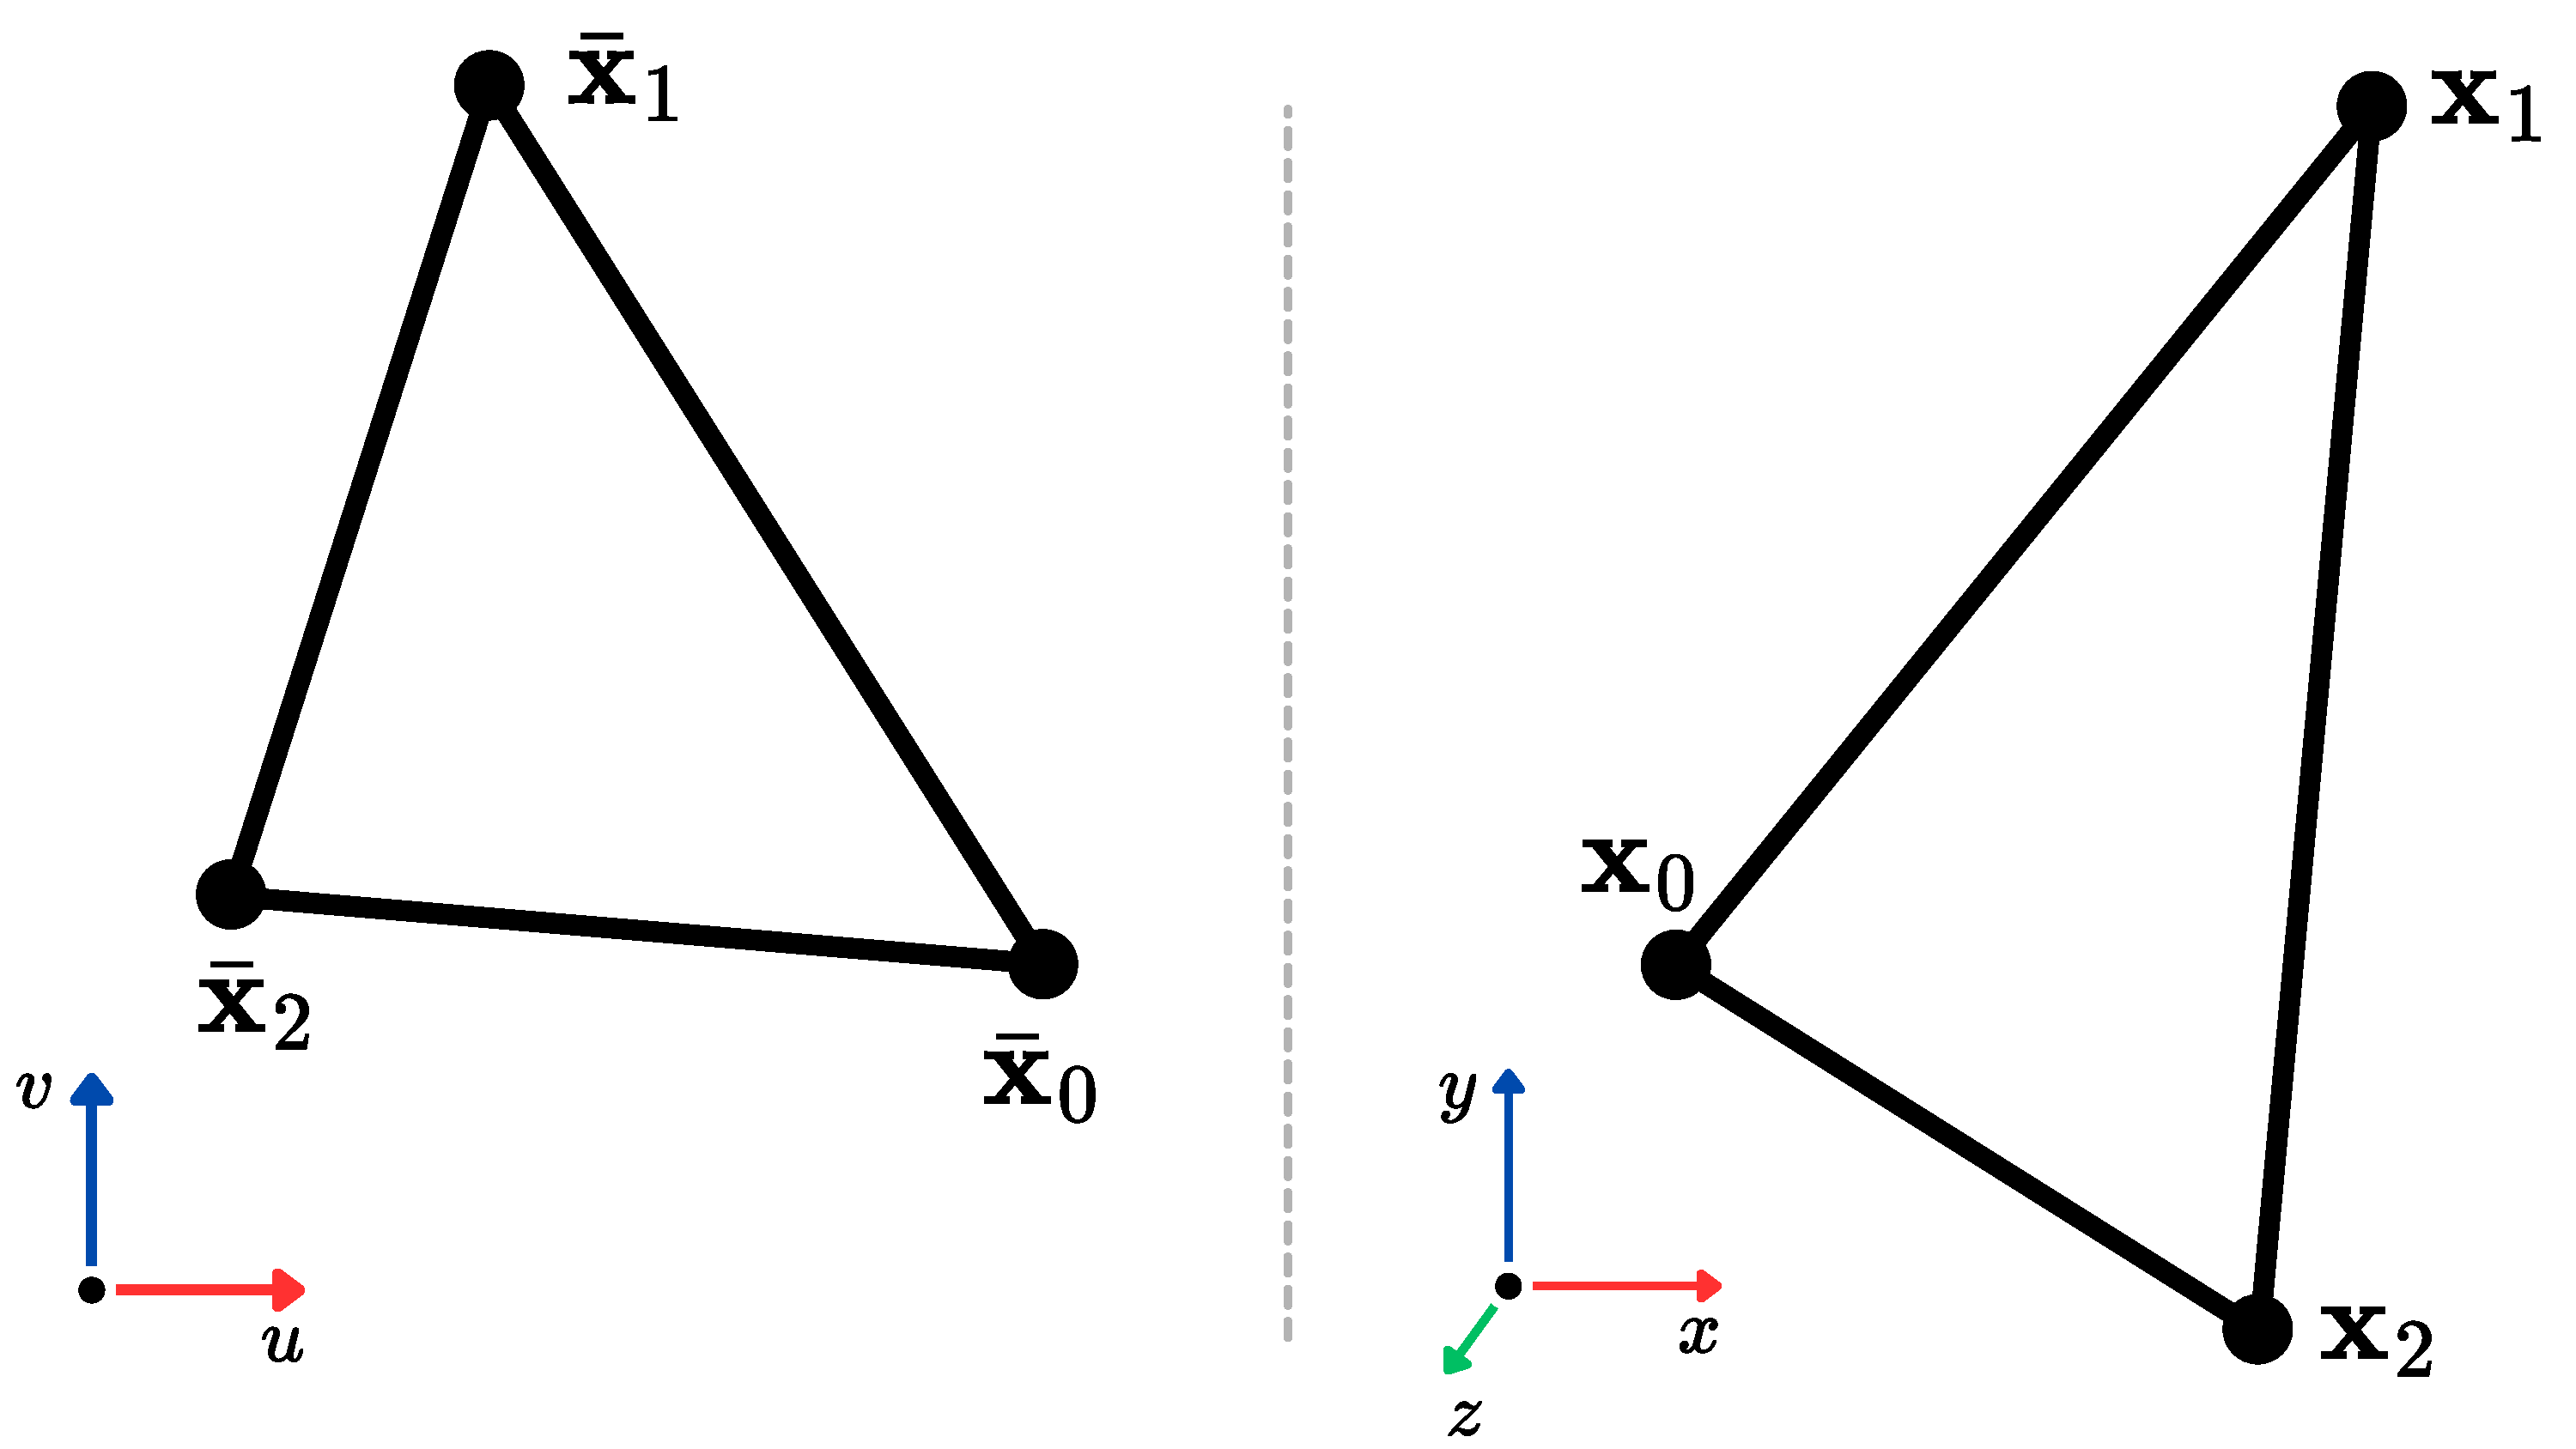
\includegraphics[width=0.85\textwidth]{images/triangles.pdf}
    \caption{Mapping of a cloth element from 2D material space coordinates $(u, v)$ to 3D world space coordinates $(x, y, z)$.}
    \label{fig:triangle_mapping}
\end{figure}

In the following we will mix the classic Baraff-Witkin notation with the one used in \cite{kim2020dynamic} and \cite{kim2020finite}. A cloth triangle is defined by its rest-state vertices $\bar{\mathbf{x}}_0, \bar{\mathbf{x}}_1, \bar{\mathbf{x}}_2 \in \mathbb{R}^2$ in material space and its world-space vertices $\mathbf{x}_0, \mathbf{x}_1, \mathbf{x}_2 \in \mathbb{R}^3$ during simulation (such that $\mathbf{x} = [\,\mathbf{x}_0 \mid \mathbf{x}_1 \mid \mathbf{x}_2\,] \in \mathbb{R}^{3 \times 3}$). We define the material and world edge matrices:
\begin{equation}
    \mathbf{D}_M = \left[ \bar{\mathbf{x}}_1 - \bar{\mathbf{x}}_0 \mid \bar{\mathbf{x}}_2 - \bar{\mathbf{x}}_0 \right] 
    \, \drop{\in \mathbb{R}^{2\times2}}
    \qquad
    \mathbf{D}_S = \left[ \mathbf{x}_1 - \mathbf{x}_0 \mid \mathbf{x}_2 - \mathbf{x}_0 \right] 
    \, \drop{\in \mathbb{R}^{3\times2}}
\end{equation}
\begin{equation}
    \mathbf{D}_M^{-1} = 
    \begin{bmatrix}
        \tilde{d}_{00} &\tilde{d}_{01} \\
        \tilde{d}_{10} &\tilde{d}_{11}
    \end{bmatrix}
    \; \drop{\in \mathbb{R}^{2 \times 2}}
\end{equation}
The deformation gradient $\mathbf{F} \in \mathbb{R}^{3\times2}$ maps material vectors 
to world-space vectors and is computed as:
\begin{equation}
    \mathbf{F} = \mathbf{D}_S \mathbf{D}_M^{-1} = \left[ \mathbf{F}_0 \mid \mathbf{F}_1 \right]
    \, \drop{\in \mathbb{R}^{3\times2}}
\end{equation}
$\mathbf{D}_M$ depends only on the rest state and is precomputed. 
The condition functions are written in terms of the columns of $\mathbf{F}$.

\noindent To compute the derivatives of the condition functions we need 
$\frac{\partial \mathbf{F}}{\partial \mathbf{x}}$. Since $\mathbf{D}_M^{-1}$ 
is constant:
\[
\pd{\mathbf{F}}{\mathbf{x}} = 
\left[ \pd{\mathbf{F}_0}{\mathbf{x}} \;\Bigg|\; \pd{\mathbf{F}_1}{\mathbf{x}} \right] = 
\pd{\mathbf{D}_S}{\mathbf{x}}\mathbf{D}_M ^{-1}
\; \drop{\in \mathbb{R}^{3 \times 2 \times 3 \times 3}}
\]
The derivatives $\frac{\partial \mathbf{D}_S}{\partial \mathbf{x}_{ij}}$ are sparse $3\times 2$ 
matrices with $\pm 1$ entries:
\begin{align*}
    \pd{\mathbf{D}_S}{\mathbf{x}_{00}} &= \begin{bmatrix} -1  &-1 \\  0  & 0 \\  0  & 0 \end{bmatrix} &
    \pd{\mathbf{D}_S}{\mathbf{x}_{01}} &= \begin{bmatrix}  1  & 0 \\  0  & 0 \\  0  & 0 \end{bmatrix} &&
    \pd{\mathbf{D}_S}{\mathbf{x}_{02}}  = \begin{bmatrix}  0  & 1 \\  0  & 0 \\  0  & 0 \end{bmatrix} \\[2ex]
    \pd{\mathbf{D}_S}{\mathbf{x}_{10}} &= \begin{bmatrix}  0  & 0 \\ -1  &-1 \\  0  & 0 \end{bmatrix} &
    \pd{\mathbf{D}_S}{\mathbf{x}_{11}} &= \begin{bmatrix}  0  & 0 \\  1  & 0 \\  0  & 0 \end{bmatrix} &&
    \pd{\mathbf{D}_S}{\mathbf{x}_{12}}  = \begin{bmatrix}  0  & 0 \\  0  & 1 \\  0  & 0 \end{bmatrix} \\[2ex]
    \pd{\mathbf{D}_S}{\mathbf{x}_{20}} &= \begin{bmatrix}  0  & 0 \\  0  & 0 \\ -1  &-1 \end{bmatrix} &
    \pd{\mathbf{D}_S}{\mathbf{x}_{21}} &= \begin{bmatrix}  0  & 0 \\  0  & 0 \\  1  & 0 \end{bmatrix} &&
    \pd{\mathbf{D}_S}{\mathbf{x}_{22}}  = \begin{bmatrix}  0  & 0 \\  0  & 0 \\  0  & 1 \end{bmatrix}
\end{align*}
where $x_{ij}$ denotes the $j$-th component of vertex $x_i$.
Multiplying by $\mathbf{D}_M^{-1}$, each block 
$\frac{\partial \mathbf{F}_k}{\partial \mathbf{x}_i} \in \mathbb{R}^{3\times3}$ 
reduces to a scalar multiple of the identity:
\begin{align*}
    \pd{\mathbf{F}_0}{\mathbf{x}_0} &= 
        -(\tilde{d}_{00} + \tilde{d}_{10})\, \mathbf{I}_{3 \times 3} &&
    \pd{\mathbf{F}_1}{\mathbf{x}_0}  = 
        -(\tilde{d}_{01} + \tilde{d}_{11})\, \mathbf{I}_{3 \times 3} \\[2ex]
    \pd{\mathbf{F}_0}{\mathbf{x}_1} &= \tilde{d}_{00}\, \mathbf{I}_{3 \times 3} &&
    \pd{\mathbf{F}_1}{\mathbf{x}_1}  = \tilde{d}_{01}\, \mathbf{I}_{3 \times 3} \\[2ex]
    \pd{\mathbf{F}_0}{\mathbf{x}_2} &= \tilde{d}_{10}\, \mathbf{I}_{3 \times 3} &&
    \pd{\mathbf{F}_1}{\mathbf{x}_2}  = \tilde{d}_{11}\, \mathbf{I}_{3 \times 3}
\end{align*}
Since all blocks are scalar multiples of $\mathbf{I}_{3 \times 3}$, we compress the coefficients into a single precomputed $3\times 2$ matrix:
\begin{equation}
\label{eq:dF_dx}
\left.\pd{\mathbf{F}}{\mathbf{x}}\right|_{\text{comp}} = 
\begin{bmatrix}
    -(\tilde{d}_{00} + \tilde{d}_{10})  & -(\tilde{d}_{01} + \tilde{d}_{11}) \\[1ex]
    \tilde{d}_{00}                      & \tilde{d}_{01}                      \\[1ex]
    \tilde{d}_{10}                      & \tilde{d}_{11}                
\end{bmatrix} \equiv
\begin{bmatrix} \hat{\mathbf{d}}_0 \mid \hat{\mathbf{d}}_1\end{bmatrix}
\;\drop{\in \mathbb{R}^{3\times 2}}
\end{equation}
so that $\frac{\partial \mathbf{F}_k}{\partial \mathbf{x}_i} = \hat{\mathbf{d}}_{ik}\,\mathbf{I}_{3 \times 3}$, where $\hat{\mathbf{d}}_{ik}$ is the $(k,i)$ entry of this matrix.

\subsection{Stretch}

Stretch along the $u$ axis is measured by how much $\|\mathbf{F}_0\|$ deviates from 1 (its rest value). The condition function, energy, and their derivatives are:
\begin{equation}
    \mathbf{C}_u(\mathbf{x}) = \|\mathbf{F}_0\| - 1\; \drop{\in \mathbb{R}}
\end{equation}
\begin{equation}
    \Psi_{\text{stretch}_u}(\mathbf{x}) = \frac{a\,k_u}{2}\,\mathbf{C}_u(\mathbf{x})^2
\end{equation}
where $a$ is the triangle's rest area in material space. The first and second derivatives with respect to vertex positions are:
\begin{equation}
    \pd{\mathbf{C}_u}{\mathbf{x}_i} = 
        \hat{\mathbf{d}}_{0i}\,\hat{\mathbf{F}}_0 
        \,\drop{\in \mathbb{R}^3}
\end{equation}
\begin{equation}
    \pdm{\mathbf{C}_u}{\mathbf{x}_i}{\mathbf{x}_j} = 
        \frac{\hat{\mathbf{d}}_{0i}\,\hat{\mathbf{d}}_{0j}}{\|\mathbf{F}_0\|}
        \left(\mathbf{I} - \hat{\mathbf{F}}_0\hat{\mathbf{F}}_0^\top\right) 
        \,\drop{\in \mathbb{R}^{3\times3}}
\end{equation}
where $\hat{\mathbf{F}}_0 = \mathbf{F}_0/\|\mathbf{F}_0\|$. The term $(\mathbf{I} - \hat{\mathbf{F}}_0\hat{\mathbf{F}}_0^\top)$ is the projection onto the plane perpendicular to $\mathbf{F}_0$. Forces, force Jacobians, and damping follow directly from equations~\ref{eq:energy_force}, \ref{eq:force_jacobian}, \ref{eq:damping_force}, \ref{eq:damping_jacobian_force} with stiffness constants $k_u$ and $\dot{k}_u$.

The $v$ axis is identical, substituting $\mathbf{F}_1$, $\hat{\mathbf{d}}_1$, and stiffness constants $k_v$, $\dot{k}_v$, allowing anisotropic material behavior.

\subsection{Shear}

Shear is measured by the inner product of the two deformation gradient columns, which is zero at rest. The condition function, energy, and derivative are:
\begin{equation}
    \mathbf{C}_s(\mathbf{x}) = \hat{\mathbf{F}}_0 \cdot \hat{\mathbf{F}}_1\, \drop{\in \mathbb{R}}
\end{equation}
\begin{equation}
    \Psi_{\text{shear}}(\mathbf{x}) = \frac{a\,k_s}{2}\,\mathbf{C}_s(\mathbf{x})^2
\end{equation}
\begin{equation}
    \pd{\mathbf{C}_s}{\mathbf{x}_i} = 
        \frac{1}{\|\mathbf{F}_0\|}\pd{\mathbf{F}_0}{\mathbf{x}_i}\text{proj}^{\perp}(\hat{\mathbf{F}}_0,\, \hat{\mathbf{F}}_1) + 
        \frac{1}{\|\mathbf{F}_1\|}\pd{\mathbf{F}_1}{\mathbf{x}_i}\text{proj}^{\perp}(\hat{\mathbf{F}}_1,\, \hat{\mathbf{F}}_0)
        \, \drop{\in \mathbb{R}^3}
\end{equation}
where $\text{proj}^{\perp}(\mathbf{a}, \hat{\mathbf{b}}) = \mathbf{a} - (\mathbf{a}\cdot\hat{\mathbf{b}})\hat{\mathbf{b}}$ 
is the component of $\mathbf{a}$ perpendicular to $\hat{\mathbf{b}}$. The second derivative $\pdm{\mathbf{C}_s}{\mathbf{x}_i}{\mathbf{x}_j}$ is not derived since the corresponding term in equation~\ref{eq:force_jacobian} is dropped for shear. Forces, Jacobians, and damping follow from equations~\ref{eq:energy_force}--\ref{eq:damping_jacobian_force} with stiffness constants $k_s$ and $\dot{k}_s$.

\subsection{Dihedral Bending}
\newcommand{\vrel}[2]{\mathbf{x}_{#1 \rightarrow #2}}

\begin{figure}[htbp] 
    \centering
    % Adjust the values below (left bottom right top)
    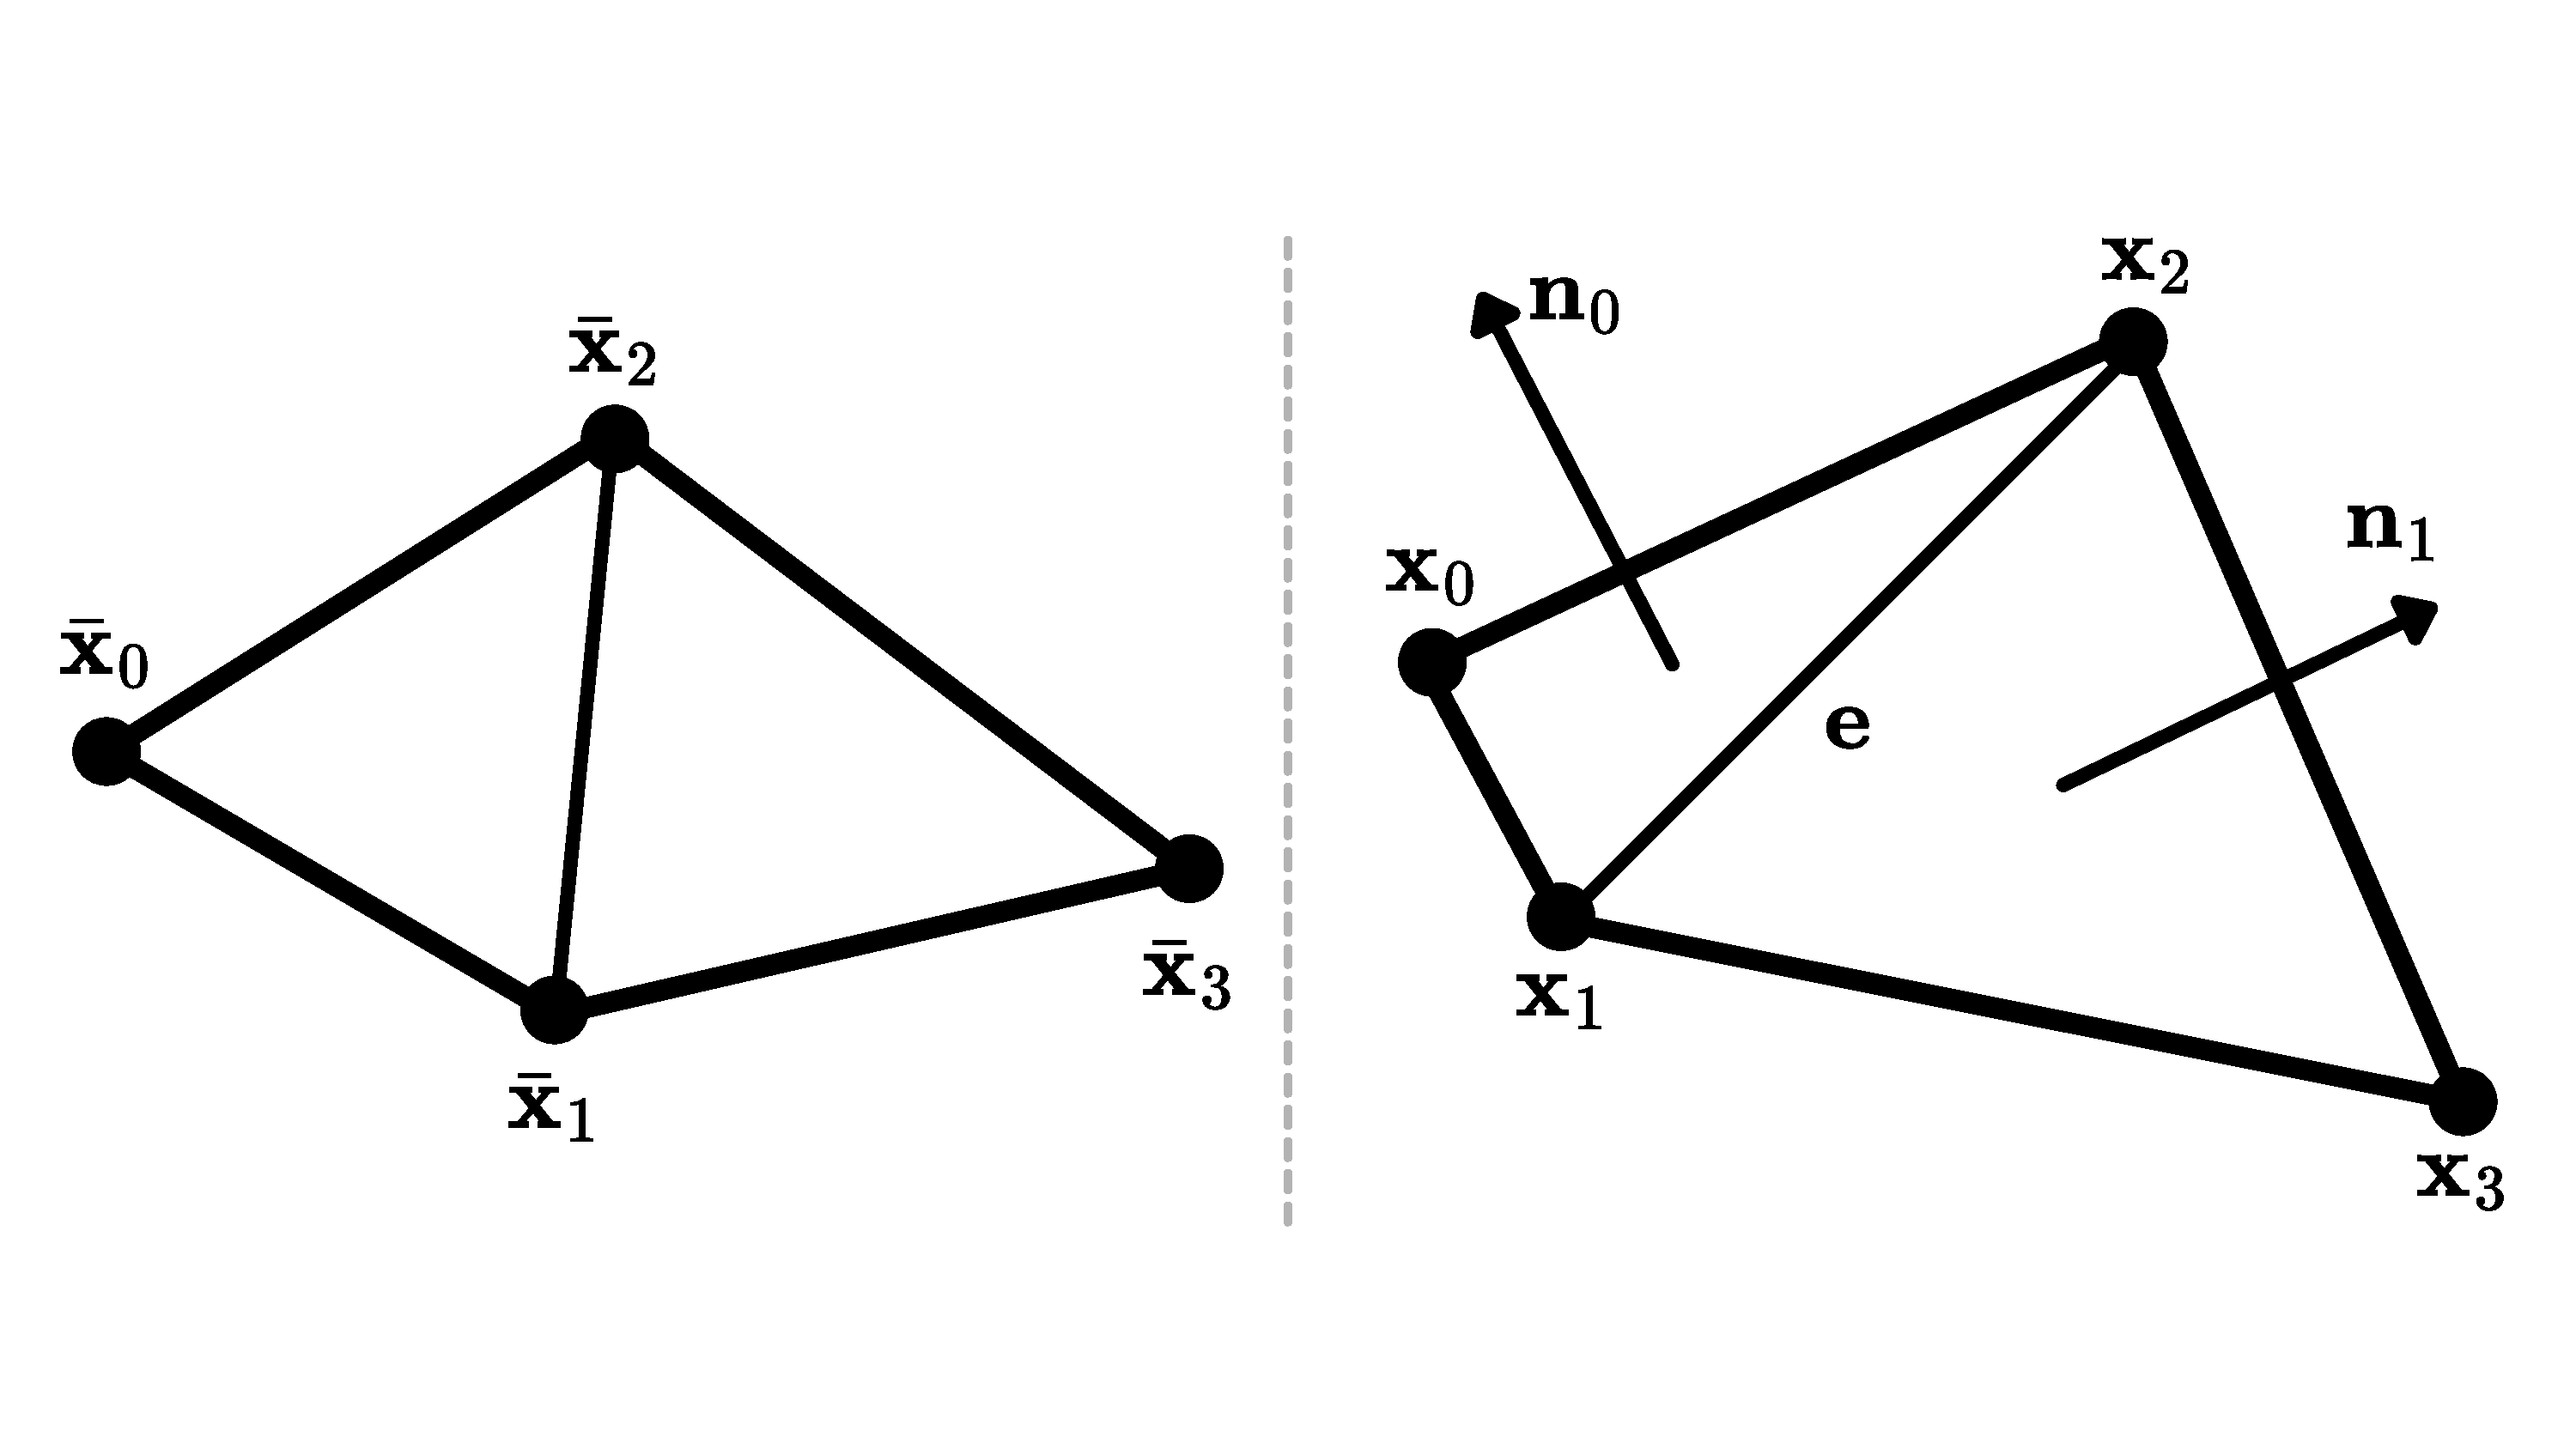
\includegraphics[width=0.9\textwidth, trim=0cm 6cm 0cm 4cm, clip]{images/dihedral.pdf}
    \caption{Geometric configuration for dihedral bending involving four vertices and two adjacent triangles.}
    \label{fig:dihedral_geometry}
\end{figure}

Bending is defined over two adjacent triangles sharing a common edge, involving 4 unique vertices. We define:
\begin{equation*}
    \vrel{i}{j} = \mathbf{x}_j - \mathbf{x}_i
    \qquad
    \mathbf{n}_0 = \vrel{0}{1} \times \vrel{0}{2}
    \qquad
    \mathbf{n}_1 = \vrel{3}{2} \times \vrel{3}{1}
\end{equation*}
\begin{equation*}
    \mathbf{e} = \vrel{1}{2}
\end{equation*}
where $\mathbf{n}_0$, $\mathbf{n}_1$ are the triangle normals and $\mathbf{e}$ 
is the shared edge. The dihedral angle $\theta$ between the two triangles 
is recovered via:
\begin{equation}
    \sin\theta = (\hat{\mathbf{n}}_0 \times \hat{\mathbf{n}}_1)\cdot\hat{\mathbf{e}}
    \qquad
    \cos\theta = \hat{\mathbf{n}}_0 \cdot \hat{\mathbf{n}}_1
    \qquad
    \theta(\mathbf{x}) = \text{arctan}\left(\frac{\sin\theta}{\cos\theta}\right)
\end{equation}
The condition, with $\theta_r$ being the rest angle, and the associated 
energy are:
\begin{equation}
    \mathbf{C}_b(\mathbf{x}) = \theta(\mathbf{x}) - \theta_r
    \, \drop{\in \mathbb{R}}
    \qquad
    \Psi_{\text{bend}}(\mathbf{x}) = \frac{k_b}{2}\,\mathbf{C}_b(\mathbf{x})^2
\end{equation}
Unlike stretch and shear, the energy is not scaled by triangle area.

\noindent The condition derivative reduces to:
\begin{equation}
\pd{\mathbf{C}_b}{\mathbf{x}_i} = \pd{\theta}{\mathbf{x}_i} = 
    \cos\theta\,\pd{\sin\theta}{\mathbf{x}_i} - 
    \sin\theta\,\pd{\cos\theta}{\mathbf{x}_i}
    \, \drop{\in \mathbb{R}^3}
\end{equation}
where:
\begin{equation}
\pd{\sin\theta}{\mathbf{x}_i} = 
\left[ 
    \frac{1}{\|\mathbf{n}_1\|}\pd{\mathbf{n}_1}{\mathbf{x}_i}\mathbf{n}_0^{\times} -
    \frac{1}{\|\mathbf{n}_0\|}\pd{\mathbf{n}_0}{\mathbf{x}_i}\mathbf{n}_1^{\times}
\right]\hat{\mathbf{e}}
\end{equation}
\begin{equation}
\pd{\cos\theta}{\mathbf{x}_i} =  
    -\frac{1}{\|\mathbf{n}_0\|}\pd{\mathbf{n}_0}{\mathbf{x}_i} 
        \text{proj}^{\perp}(\hat{\mathbf{n}}_1, \hat{\mathbf{n}}_0) -
    \frac{1}{\|\mathbf{n}_1\|}\pd{\mathbf{n}_1}{\mathbf{x}_i} 
        \text{proj}^{\perp}(\hat{\mathbf{n}}_0, \hat{\mathbf{n}}_1)
\end{equation}
The normal Jacobians $\frac{\partial \mathbf{n}_k}{\partial \mathbf{x}_i} \in \mathbb{R}^{3\times3}$ are skew-symmetric matrices:
\begin{equation}
\begin{alignedat}{4}
    &\pd{\mathbf{n}_0}{\mathbf{x}_0} = \mathbf{e}^{\times} \quad& 
    &\pd{\mathbf{n}_0}{\mathbf{x}_1} = \vrel{2}{0}^{\times} \quad&
    &\pd{\mathbf{n}_0}{\mathbf{x}_2} = \vrel{0}{1}^{\times} \quad&
    &\pd{\mathbf{n}_0}{\mathbf{x}_3} = \mathbf{0}           \\[1ex]
    &\pd{\mathbf{n}_1}{\mathbf{x}_0} = \mathbf{0} \quad& 
    &\pd{\mathbf{n}_1}{\mathbf{x}_1} = -\mathbf{e}^{\times} \quad&
    &\pd{\mathbf{n}_1}{\mathbf{x}_2} = \vrel{3}{2}^{\times} \quad&
    &\pd{\mathbf{n}_1}{\mathbf{x}_3} = \vrel{1}{3}^{\times}
\end{alignedat}
\end{equation}
where $v^{\times}$ denotes the skew-symmetric cross-product matrix of $v$:
\begin{equation*}
v^\times = 
\begin{bmatrix}
     0  & -v_2 &  v_1 \\
     v_2&    0 & -v_0 \\
    -v_1&  v_0 &    0
\end{bmatrix}
\end{equation*}
Second derivatives $\pdm{\theta}{\mathbf{x}_i}{\mathbf{x}_j}$ are not derived as the corresponding term in equation~\ref{eq:force_jacobian} is dropped.

\newpage

\section{Descent Methods \cite{wang2016descent}}
\label{sec:descent_methods}

We start from the variational form of implicit Euler time integration for an elastic deformable body:
\begin{equation}
\begin{gathered}
    g(\mathbf{x}) = \frac{1}{2h^2}(\mathbf{x} - \tilde{\mathbf{x}})^\top \mathbf{M} (\mathbf{x} - \tilde{\mathbf{x}}) + \sum_i U_i(\mathbf{x}) \\[1ex]
    \mathbf{x}^+ = \arg\min_{\mathbf{x}} g(\mathbf{x})
\end{gathered}
\end{equation}
where $\tilde{\mathbf{x}} = \mathbf{x}^- + h\mathbf{v}^- + h^2\mathbf{M}^{-1}\mathbf{f}_{\text{ext}}$ is the inertial predictor. A descent method solves this minimization iteratively: starting from an initial guess $\mathbf{x}^{(0)}$, each iterate is updated as
\begin{equation}
    \mathbf{x}^{(k+1)} = \mathbf{x}^{(k)} + \alpha^{(k)} \Delta\mathbf{x}^{(k)}, 
    \qquad
    \Delta\mathbf{x}^{(k)} \cdot \nabla g(\mathbf{x}^{(k)}) < 0
\end{equation}
The descent condition on the right ensures $g$ decreases locally along $\Delta\mathbf{x}^{(k)}$ for sufficiently small $\alpha^{(k)}$. Different descent methods correspond to different choices of $\Delta\mathbf{x}^{(k)}$ and $\alpha^{(k)}$, and optionally a momentum-based acceleration step. The general structure is:

\begin{algorithm}[H]
\label{alg:descent_timestep}
\caption{General Descent Method Time Step}
\begin{algorithmic}[1]
\Function{DescentTimestep}{$\mathbf{x}^-, \mathbf{v}^-, h$}
    \State Initialize $\mathbf{x}^{(0)}$
    \For{$k = 0, 1, 2, \dots$}
        \State $\Delta\mathbf{x}^{(k)} \gets \textsc{ComputeDescentDirection}()$
        \State $\alpha^{(k)} \gets \textsc{ComputeStepLength}()$
        \State $\bar{\mathbf{x}}^{(k+1)} \gets \mathbf{x}^{(k)} + \alpha^{(k)}\Delta\mathbf{x}^{(k)}$
        \State $\mathbf{x}^{(k+1)} \gets \textsc{Acceleration}(\bar{\mathbf{x}}^{(k+1)}, \bar{\mathbf{x}}^{(k)}, \mathbf{x}^{(k)}, \mathbf{x}^{(k-1)})$
    \EndFor
    \State \Return $\mathbf{x}^{(k)}$
\EndFunction
\end{algorithmic}
\end{algorithm}

\subsection{Existing Methods as Descent Methods}

Many existing simulation methods can be cast as descent methods within the framework of Algorithm \ref{alg:descent_timestep}, differing only in their choice of descent direction $\Delta\mathbf{x}^{(k)}$.

\newlength{\lhswidth}
\settowidth{\lhswidth}{$\displaystyle \Delta\mathbf{x}^{(k)} = -\mathbf{J}^{(k)} + \frac{z^{(k)}}{z^{(k-1)}}\Delta\mathbf{x}^{(k-1)}$}
\addtolength{\lhswidth}{1em}
\newlength{\rhswidth}
\settowidth{\rhswidth}{$\displaystyle \mathbf{J}^{(k)} = \nabla g(\mathbf{x}^{(k)})$}
\addtolength{\rhswidth}{1em}
\newcommand{\eqlhs}[1]{\makebox[\lhswidth][l]{$\displaystyle #1$}}
\newcommand{\eqrhs}[1]{\makebox[\rhswidth][l]{$\displaystyle #1$}}

\paragraph{Gradient Descent.}
Step in the direction of steepest decrease. Cheap per iteration but slow to converge on ill-conditioned problems.
\begin{equation}
    \eqlhs{\Delta\mathbf{x}^{(k)} = -\mathbf{J}^{(k)}}
    \quad \text{with }\;
    \eqrhs{\mathbf{J}^{(k)} = \nabla g(\mathbf{x}^{(k)})}
\end{equation}

\paragraph{Newton.}
Locally approximates $g$ as a quadratic and jumps to its minimum. Quadratic convergence, but each iteration requires solving a $3n \times 3n$ linear system.
\begin{equation}
    \eqlhs{\Delta\mathbf{x}^{(k)} = -[\mathbf{H}^{(k)}]^{-1}\mathbf{J}^{(k)}}
    \quad \text{with }\;
    \eqrhs{\mathbf{H}^{(k)} = \nabla^2 g(\mathbf{x}^{(k)})}
\end{equation}

\paragraph{Quasi-Newton.}
Replaces $[\mathbf{H}^{(k)}]^{-1}$ with a cheaper SPD approximation $\mathbf{P}^{(k)}$ that avoids or simplifies the linear solve, trading convergence rate for per-iteration cost.
\begin{equation}
    \eqlhs{\Delta\mathbf{x}^{(k)} = -\mathbf{P}^{(k)}\mathbf{J}^{(k)}}
    \quad \text{with }\;
    \eqrhs{\mathbf{P}^{(k)} \approx [\mathbf{H}^{(k)}]^{-1}}
\end{equation}

\paragraph{Nonlinear Conjugate Gradient.}
Adds a momentum term to gradient descent, weighted by the Fletcher–Reeves coefficient $z^{(k)}/z^{(k-1)}$, requires dot products at every iteration.
\begin{equation}
    \eqlhs{\Delta\mathbf{x}^{(k)} = -\mathbf{J}^{(k)} + \frac{z^{(k)}}{z^{(k-1)}}\Delta\mathbf{x}^{(k-1)}}
    \quad \text{with }\;
    \eqrhs{z^{(k)} = \mathbf{J}^{(k)} \cdot \mathbf{J}^{(k)}}
\end{equation}

\paragraph{Projective Dynamics~\cite{bouaziz2023projective}.}
A Quasi-Newton method applied to the augmented PD energy $g_{\text{PD}}$, where $\mathbf{L}$ is a constant Hessian approximation evaluated at the rest configuration. Since $\mathbf{L}$ never changes, it can be Cholesky-factorized once at initialization, reducing each iteration to a back-substitution.
\begin{equation}
    \eqlhs{\Delta\mathbf{x}^{(k)} = -\mathbf{L}^{-1}\nabla g_{\text{PD}}^{(k)}}
    \quad \text{with }\;
    \eqrhs{\mathbf{L} \approx \mathbf{H}}
\end{equation}

\paragraph{Baraff-Witkin~\cite{baraff1998large}.}
One iteration of Newton's method ($k = 1$) with no further refinement. Fast but inexact: the implicit Euler equation is only approximately satisfied per timestep.
\begin{equation}
    \eqlhs{\Delta\mathbf{x} = -\mathbf{H}^{-1}\mathbf{J}}
    \quad \text{with }\;
    \eqrhs{k = 1}
\end{equation}

\subsection{Jacobi-Preconditioned Gradient Descent with Chebyshev Acceleration}

The method proposed by~\cite{wang2016descent} is designed to be GPU-friendly: every operation is element-wise and reduction-free.

\paragraph{Descent direction.}
A Quasi-Newton step with the Jacobi preconditioner, i.e.\ the inverse diagonal of the Hessian:
\begin{equation}
    \Delta\mathbf{x}^{(k)} = -\textsc{diag}(\mathbf{H}^{(k)})^{-1}\mathbf{J}^{(k)}
\end{equation}
The preconditioner is trivial to invert (element-wise reciprocal), avoiding the linear solve required by full Newton or Quasi-Newton methods. This approximation is effective for elastic problems because the Hessian is diagonally dominant: $\mathbf{H} = \mathbf{M} + h^2 \mathbf{J}^\top\mathbf{K}\mathbf{J}$, where $\mathbf{M}$ is already exactly diagonal and the elastic term aggregates per-element contributions whose diagonal entries dominate the off-diagonals.

\paragraph{Chebyshev acceleration.}
On top of each descent step, a momentum-based correction blends the current iterate with the one two steps prior:
\begin{equation}
    \mathbf{x}^{(k+1)} = \omega^{(k+1)}\bigl(\bar{\mathbf{x}}^{(k+1)} - \mathbf{x}^{(k-1)}\bigr) + \mathbf{x}^{(k-1)}
\end{equation}
where $\bar{\mathbf{x}}^{(k+1)} = \mathbf{x}^{(k)} + \alpha^{(k)}\Delta\mathbf{x}^{(k)}$ is the raw descent update and the scalar coefficient $\omega^{(k+1)}$ evolves as:
\begin{equation}
    \omega^{(k+1)} = \frac{4}{4 - \rho^2\,\omega^{(k)}}, \qquad \omega^{(1)} = 1
\end{equation}
The parameter $\rho \in (0,1)$ controls how aggressive the acceleration is: values close to $1$ speed up convergence the most but can cause the iteration to diverge. 

% \paragraph{Step length.}
% A relaxed Wolfe condition without dot products: accept $\alpha^{(k)}$ if the energy decreases, $g(\mathbf{x}^{(k)} + \alpha^{(k)}\Delta\mathbf{x}^{(k)}) < g(\mathbf{x}^{(k)})$. Energy is checked only every 8 iterations and warm-started from the previous timestep's final $\alpha$.

\paragraph{Initialization.}
$\mathbf{x}^{(0)}$ is predicted from the previous two timesteps assuming constant acceleration: $\mathbf{x}^{(0)} = \mathbf{x}^- + h\mathbf{v}^- + \eta h(\mathbf{v}^- - \mathbf{v}^{--})$ with damping $\eta \approx 0.2$.

%The key advantage over alternatives like Nonlinear CG is that this update is fully element-wise: it requires no dot products and parallelizes perfectly on the GPU.

\newpage

\section{Primal/Dual Descent Methods \cite{macklin2020primal}}
\label{sec:primal_dual}

Following the Article \cite{macklin2020primal}, we derive a variational formulation of implicit Euler time integration for deformable bodies. Starting from the equations of motion, we cast the time step as a minimization problem (the primal objective), then derive its Lagrangian dual and show how Newton descent on the dual yields an efficient per-constraint update rule that forms the basis of XPBD.

\subsection{Equations of Motion}

For a deformable body, the discrete equations of motion are defined by the implicit system:
\begin{equation}
    \mathbf{M}(\mathbf{v}_{t+1} - \tilde{\mathbf{v}}) - h\,\mathbf{f}(\mathbf{x}_{t+1}, \mathbf{v}_{t+1}) = \mathbf{0}
\end{equation}
where the \textit{unconstrained velocity} $\tilde{\mathbf{v}}$ represents the state of the system under external forces alone:
\begin{equation}
    \tilde{\mathbf{v}} = \mathbf{v}_t + h \mathbf{M}^{-1} \mathbf{f}_{\text{ext}}
\end{equation}

\begin{derivation}
Starting from Newton's second law $\mathbf{M}\ddot{\mathbf{x}} = \mathbf{f}(\mathbf{x}, \dot{\mathbf{x}})$, we introduce $\mathbf{v} = \dot{\mathbf{x}}$ 
to rewrite the continuous equations of motion as a first-order system:
%
\begin{equation*}
    \dot{\mathbf{x}} = \mathbf{v}, 
    \qquad 
    \mathbf{M}\dot{\mathbf{v}} = \mathbf{f}(\mathbf{x}, \mathbf{v})
\end{equation*}
%
Forces are split into external (non-stiff) and internal (stiff) contributions:
%
\begin{equation*}
    \mathbf{f}(\mathbf{x}, \mathbf{v}) = \mathbf{f}_{\text{ext}} + 
    \mathbf{f}_{\text{int}}(\mathbf{x}, \mathbf{v})
\end{equation*}
%
Applying implicit Euler:
%
\begin{equation*}
\begin{aligned}
    \mathbf{x}_{t+1} &= \mathbf{x}_t + h\,\mathbf{v}_{t+1}
    \\[1ex]
    \mathbf{M}\,\mathbf{v}_{t+1} &= \mathbf{M}\,\mathbf{v}_t + 
    h\,\mathbf{f}_{\text{ext}} + h\,\mathbf{f}_{\text{int}}(\mathbf{x}_{t+1}, \mathbf{v}_{t+1})
\end{aligned}
\end{equation*}
%
Collecting all known quantities on the right-hand side and defining 
the \textit{unconstrained velocity}:
%
\begin{equation*}
    \tilde{\mathbf{v}} \equiv \mathbf{v}_t + h\,\mathbf{M}^{-1}\mathbf{f}_{\text{ext}}
    \qquad \Longleftrightarrow \qquad
    \mathbf{M}\,\tilde{\mathbf{v}} = \mathbf{M}\,\mathbf{v}_t + h\,\mathbf{f}_{\text{ext}}
\end{equation*}
%
substituting into the velocity equation and writing 
$\mathbf{f} \equiv \mathbf{f}_{\text{int}}$ gives:
%
\begin{equation*}
    \mathbf{M}\,\mathbf{v}_{t+1} - h\,\mathbf{f}(\mathbf{x}_{t+1}, \mathbf{v}_{t+1}) 
    = \mathbf{M}\,\tilde{\mathbf{v}}
\end{equation*}
\begin{equation*}
    \mathbf{M}(\mathbf{v}_{t+1} - \tilde{\mathbf{v}}) - 
    h\,\mathbf{f}(\mathbf{x}_{t+1},\mathbf{v}_{t+1}) = \mathbf{0}
\end{equation*}
\end{derivation}

\subsection{The Primal Objective}

The primal optimization problem that encodes the implicit Euler time integration scheme is defined by the objective function $g(\mathbf{v})$:
\begin{equation}
    g(\mathbf{v}) = \frac{1}{2}(\mathbf{v} - \tilde{\mathbf{v}})^\top \mathbf{M} (\mathbf{v} - \tilde{\mathbf{v}}) + \sum_i U_i(\mathbf{x}_{t+1}(\mathbf{v}))
\end{equation}
where the dependence of the potential energy on the velocity is defined through the position update:
\begin{equation}
    \mathbf{x}_{t+1}(\mathbf{v}) = \mathbf{x}_t + h \mathbf{v}
\end{equation}
The velocity for the next time step is then found by minimizing this objective:
\begin{equation}
    \mathbf{v}_{t+1} = \arg \min_{\mathbf{v}} g(\mathbf{v})
\end{equation}

\subsection{Quadratic Potentials}

Restricting our model to quadratic potentials, a single elastic energy term takes the form:
\begin{equation}
    U_i = \frac{1}{2}\, k_i\, \mathbf{C}_i(\mathbf{x})^2
    \; \red{\in \mathbb{R}}
    \qquad
    U = \frac{1}{2}\, \mathbf{C}(\mathbf{x})^\top\, \mathbf{K}\, \mathbf{C}(\mathbf{x})
    \; \red{\in \mathbb{R}}
\end{equation}
where $\mathbf{K} = \textsc{diag}([k_1, k_2, \dots, k_m])\; \red{\in \mathbb{R}^{m\times m}}$ is the stiffness coefficients matrix and $\mathbf{C}(\mathbf{x}) = [\mathbf{C}_1(\mathbf{x}), \mathbf{C}_2(\mathbf{x}), \dots, \mathbf{C}_m(\mathbf{x})]\; \red{\in \mathbb{R}^m}$ is the constraint function evaluation column vector. Defining the constraints Jacobian as:
\begin{equation}
    \mathbf{J}_i = \pd{\mathbf{C}_i}{\mathbf{x}}
     \; \red{\in \mathbb{R}^{1 \times 3n}}
     \qquad
     \mathbf{J} = \pd{\mathbf{C}}{\mathbf{x}}
     \; \red{\in \mathbb{R}^{m \times 3n}}
\end{equation}
The generalized elastic force arising from a single potential $U_i$ is given by the negative gradient:
\begin{equation}
    \mathbf{f}_i = -\left(\pd{U_i}{\mathbf{x}}\right)^\top = -k_i\, \mathbf{J}_i^\top \mathbf{C}_i(\mathbf{x})
    \; \red{\in \mathbb{R}^{3n}}
\end{equation}
and the full force vector arising from all the potentials $U$:
\begin{equation}
    \mathbf{f} = -\left(\pd{U}{\mathbf{x}}\right)^\top =
    - \mathbf{J}^\top \mathbf{K}\, \mathbf{C}(\mathbf{x})
    \; \red{\in \mathbb{R}^{3n}}
\end{equation}
%
To solve the minimization problem trough Newton's method we need first and second derivative of $g$ with respect to $\mathbf{v}$:
%
\begin{equation}
\begin{aligned}
    \pd{g}{\,\mathbf{v}} &=  \bigg[\; \mathbf{M} (\mathbf{v} - \tilde{\mathbf{v}}) + h\,\mathbf{J}^\top \mathbf{K}\, \mathbf{C}(\mathbf{x}_{t+1}(\mathbf{v}))\; \bigg]
    \;&&\red{\in \mathbb{R}^{3n}} \\[2ex]
    \pdv{g}{\,\mathbf{v}} &= \bigg[\; \mathbf{M} + h^2\, \mathbf{J}^\top \mathbf{K}\, \mathbf{J} \; \bigg]
    \;&&\red{\in \mathbb{R}^{3n \times 3n}}
\end{aligned}
\end{equation}


\begin{derivation}
The objective $g$ can be split into two terms:
%
\begin{equation*}
    g(\mathbf{v}) = g_{\text{inertia}}(\mathbf{v}) + g_{\text{elastic}}(\mathbf{v})
\end{equation*}
%
The Jacobian and Hessian decompose accordingly:
%
\begin{equation*}
    \pd{g}{\,\mathbf{v}} = 
    \pd{g_{\text{inertia}}}{\,\mathbf{v}} +
    \pd{g_{\text{elastic}}}{\,\mathbf{v}}\, ,
    \qquad
    \pdv{g}{\,\mathbf{v}} = 
    \pdv{g_{\text{inertia}}}{\,\mathbf{v}} +
    \pdv{g_{\text{elastic}}}{\,\mathbf{v}}
\end{equation*}

\paragraph{Inertia term.}
The inertia term is a quadratic form in $\mathbf{v}$, so its Jacobian and Hessian are simply:
%
\begin{equation*}
    \pd{g_{\text{inertia}}}{\mathbf{v}} =     
    \pd
    {\left[ \dfrac{1}{2}(\mathbf{v} - \tilde{\mathbf{v}})^\top \mathbf{M} (\mathbf{v} - \tilde{\mathbf{v}}) \right]}
    {\mathbf{v}} 
    = \mathbf{M} (\mathbf{v} - \tilde{\mathbf{v}})
\end{equation*}
\begin{equation*}
    \pdv{g_{\text{inertia}}}{\mathbf{v}}
    = \pd{\;\mathbf{M} (\mathbf{v} - \tilde{\mathbf{v}})}{\mathbf{v}} 
    = \mathbf{M}
\end{equation*}

\paragraph{Elastic term.}
Applying the chain rule through $\mathbf{x}_{t+1} = \mathbf{x}_t + h\mathbf{v}$, 
the first derivative of $U$ with respect to $\mathbf{v}$ is:
%
\begin{equation*} 
    \pd{U(\mathbf{x}_{t+1}(\mathbf{v}))}{\mathbf{v}} 
    = 
    \pd{\mathbf{x}_{t+1}}{\mathbf{v}} \pd{U}{\mathbf{x}_{t+1}} 
    = 
    h\, \pd{U}{\mathbf{x}}(\mathbf{x}_{t+1}) 
    = 
    h\, \mathbf{J}^\top \mathbf{K}\, \mathbf{C}(\mathbf{x}_{t+1})
\end{equation*}
%
So first derivative of the elastic term is symply:
\begin{equation*} 
\pd{g_{\text{elastic}}}{\mathbf{v}} = 
    \pd{U}{\mathbf{v}} =
    h\, \mathbf{J}^\top \mathbf{K}\, \mathbf{C}(\mathbf{x}_{t+1})
\end{equation*}
%
Differentiating once more with respect to $\mathbf{v}$, applying the chain rule a second time:
%
\begin{equation*}
    \pdv{g_{\text{elastic}}}{\mathbf{v}} = 
    \pdv{U(\mathbf{x}_{t+1})}{\mathbf{v}} = 
    h\, \pd{\left[\pd{U}{\mathbf{x}}(\mathbf{x}_{t+1})\right]}{\mathbf{v}} = 
    h^2\, \pdv{U}{\mathbf{x}}
\end{equation*}
%
The second derivative of $U$ with respect to positions expands as:
%
\begin{equation*}
    \pdv{U}{\mathbf{x}} = 
    \mathbf{J}^\top \mathbf{K}\, \mathbf{J} + 
    \drop{\sum_{i} k_i\, \pdv{\mathbf{C}_i}{\mathbf{x}}\mathbf{C}_i(\mathbf{x})}
\end{equation*}
%
The \red{red} term is usually dropped. Combining both contributions, the full Hessian of $g$ with respect to $\mathbf{v}$ is:
%
\begin{equation*}
    \pd{^2 g}{\mathbf{v}^2} = \mathbf{M} + h^2\, \mathbf{J}^\top \mathbf{K}\, \mathbf{J}
\end{equation*}
\end{derivation}

\subsection{Newton Descent}
\label{sec:newton_method}

The exact Newton update for $\mathbf{v}$ at iteration $k$ is:
\begin{equation}
    \mathbf{v}^{k+1} = \mathbf{v}^k - \alpha\,\mathbf{H}^{-1}\,\pd{g}{\mathbf{v}}
\end{equation}
where $\mathbf{H} = \pdc{^2g}{\mathbf{v}^2} = \mathbf{M} + h^2\mathbf{J}^\top\mathbf{K}\mathbf{J}$ is recomputed at each iteration. This converges quadratically, but requires solving an $3n \times 3n$ linear system at each step.

\paragraph{Quasi-Newton.}
Since $\mathbf{H}^{-1}$ is expensive to compute, one replaces it with a 
symmetric positive definite approximation $\mathbf{P} \approx \mathbf{H}^{-1}$:
\begin{equation}
    \mathbf{v}^{k+1} = \mathbf{v}^k - \alpha\,\mathbf{P}\,\pd{g}{\mathbf{v}}
\end{equation}
Convergence usually degrades from quadratic to linear, but each iteration costs 
less.

\paragraph{Diagonal preconditioner.}
The simplest choice is the inverse diagonal of $\mathbf{H}$:
\begin{equation}
\label{eq:diagonal_prec}
    \mathbf{P}_{dd} = \frac{1}{\mathbf{M}_{dd} + h^2\,\mathbf{J}_d^\top \mathbf{K}\,\mathbf{J}_d}
\end{equation}
where $d$ indexes the diagonal entries and $\mathbf{J}_d \in \mathbb{R}^m$ is the $d$-th column of $\mathbf{J}$, collecting the derivatives of all constraints with respect to DOF $d$.

\begin{algorithm}[H]
\caption{Primal Descent Time Step}
\begin{algorithmic}[1]
\Function{PrimalStep}{$\mathbf{x}_t,\, \mathbf{v}_t,\, \mathbf{M},\, \mathbf{K},\, h$}
    \State $\mathbf{v} \gets \tilde{\mathbf{v}}$ 
    \hfill $\red{\in \mathbb{R}^{3n}}$
    \State $\mathbf{x} \gets \mathbf{x}_t + h\mathbf{v}$ 
    \hfill $\red{\in \mathbb{R}^{3n}}$
    \For{$k$ iterations}
        \State $\mathbf{f} \gets \mathbf{0}$ 
        \hfill $\red{\in \mathbb{R}^{3n}}$
        \State $\mathbf{p} \gets \mathbf{0}$ 
        \hfill $\red{\in \mathbb{R}^{3n}}$
        \For{$i$ forces}
            \State $\mathbf{f} \gets \mathbf{f} + h\,\mathbf{J}_i^\top\,k_{i}\, \mathbf{C}_i(\mathbf{x})$
            \State $\mathbf{p} \gets \mathbf{p} + \textsc{diag}(h^2\,\mathbf{J}_i^\top\,k_{i}\,\mathbf{J}_i)$
        \EndFor
    \State $\mathbf{d} \gets \mathbf{M}(\mathbf{v} - \tilde{\mathbf{v}}) + \mathbf{f}$
    \hfill $\red{\in \mathbb{R}^{3n}}$
    \State $\mathbf{P} \gets (\mathbf{M} + \textsc{diag}(\mathbf{p}))^{-1}$
    \hfill $\red{\in \mathbb{R}^{3n \times 3n}}$
    \State $\mathbf{v} \gets \mathbf{v} - \mathbf{P}\mathbf{d}$
    \State $\mathbf{x} \gets \mathbf{x}_t + h\mathbf{v}$
    \EndFor
\EndFunction
\end{algorithmic}
\end{algorithm}

\subsection{Collision and Friction}
\label{sec:primal_collision_friction}

\subsubsection{Collision}
\paragraph{Collision constraint.}
For a candidate contact pair, we define the signed-gap constraint:
\begin{equation}
    \mathbf{C}_i(\mathbf{x}) = \mathbf{n}^\top\bigl[\mathbf{a}_i(\mathbf{x}) - \mathbf{b}_i(\mathbf{x})\bigr] - d \;\red{\in \mathbb{R}}
\end{equation}
where $\mathbf{a}_i(\mathbf{x}), \mathbf{b}_i(\mathbf{x})\; \red{\in \mathbb{R}^3}$ are the closest points on the two colliding primitives (point-triangle or edge-edge), $\mathbf{n}\;\red{\in \mathbb{R}^3}$ is the contact normal, and $d$ is the collision thickness. Non-penetration corresponds to $\mathbf{C}_i(\mathbf{x}) \geq 0$.

\paragraph{Penalty potential.}
We enforce non-penetration through a one-sided polynomial potential that activates only under interpenetration:
\begin{equation}
    U_i(\mathbf{x}) = \frac{k_i}{p}\,\min\bigl(0,\, \mathbf{C}_i(\mathbf{x})\bigr)^p
\end{equation}
where $k_i > 0$ is the contact stiffness and $p \geq 2$ is a fixed exponent. The case $p = 2$ recovers the standard quadratic penalty consistent with the elastic potentials of the previous section; higher $p$ yields smoother derivatives at the activation boundary. As $k_i \to \infty$ the potential approaches hard contact.

\paragraph{Force and Jacobian approximation.}
The contact force is the negative gradient of $U_i$:
\begin{equation}
    \mathbf{f}_i = -k_i\, \mathbf{J}_i^\top\, \min\bigl(0, \mathbf{C}_i(\mathbf{x})\bigr)^{p-1}
    \;\red{\in \mathbb{R}^{3n}}
\end{equation}
with $\mathbf{J}_i = \pdc{\mathbf{C}_i}{\mathbf{x}} \in \mathbb{R}^{1 \times 3n}$ the constraint Jacobian. Dropping the geometric-stiffness term the force Jacobian needed for the preconditioner reduces to:
\begin{equation}
    \pd{\mathbf{f}_i}{\mathbf{x}} \approx
    \begin{cases}
        -k_i\,(p-1)\,\mathbf{J}_i^\top \mathbf{J}_i\, \min\bigl(0, \mathbf{C}_i(\mathbf{x})\bigr)^{p-2}
        & \mathbf{C}_i(\mathbf{x}) < 0 \\[1ex]
        \mathbf{0} & \mathbf{C}_i(\mathbf{x}) \geq 0
    \end{cases}
    \quad\red{\in \mathbb{R}^{3n\times3n}}
\end{equation}
This approximation preserves positive semi-definiteness, ensuring the descent direction remains valid, and is justified by re-evaluation of $\mathbf{J}_i$ and $\mathbf{C}_i$ at each iteration.

\subsubsection{Friction}

Let $\mathbf{D} = [\mathbf{t}_1 \mid \mathbf{t}_2] \;\red{\in \mathbb{R}^{3 \times 2}}$ be the tangent-plane basis at the contact, with $\mathbf{t}_1, \mathbf{t}_2$ unit vectors orthogonal to the normal $\mathbf{n}$. Given the relative velocity $\bar{\mathbf{v}} \in \mathbb{R}^3$ of the two contacting primitives, the slip velocity is $\bar{\mathbf{v}}_s = \mathbf{D}^\top \bar{\mathbf{v}} \;\red{\in \mathbb{R}^2}$.

\paragraph{Penalty potential.}
We define a velocity-dependent friction potential with stick and slip regimes separated by the Coulomb threshold $\mu|\mathbf{f}_n|$:
\begin{equation}
    U_f(\mathbf{v}) = 
    \begin{cases}
        \tfrac{1}{2}\,k_f\,|\bar{\mathbf{v}}_s|^2 
        & k_f|\bar{\mathbf{v}}_s| < \mu|\mathbf{f}_n| \quad\text{(stick)} \\[1ex]
        \mu|\mathbf{f}_n|\,|\bar{\mathbf{v}}_s| - \gamma 
        & \text{otherwise} \quad\qquad\text{(slip)}
    \end{cases}
\end{equation}
where $\mathbf{f}_n$ is the normal contact force (treated as a lagged parameter) and $\gamma = \mu^2|\mathbf{f}_n|^2/(2k_f)$ ensures $C^0$ continuity at the transition. 

\paragraph{Force.}
The friction force is the negative gradient of $U_f$:
\begin{equation}
    \mathbf{f}_f = -\min\!\left(k_f,\; \mu\frac{|\mathbf{f}_n|}{|\bar{\mathbf{v}}_s|}\right) \mathbf{D}\mathbf{D}^\top \bar{\mathbf{v}}
    \;\red{\in \mathbb{R}^3}
\end{equation}

\paragraph{Preconditioner.}
The Hessian factorizes as:
\begin{equation}
    \pd{\mathbf{f}_f}{\mathbf{v}} = -\mathbf{D}\,\boldsymbol{\Lambda}\,\mathbf{D}^\top
\end{equation}
with:
\begin{equation}
    \boldsymbol{\Lambda} = 
    \begin{cases}
        k_f\,\mathbf{I}_{2\times 2} \\[1ex]
        \mu\dfrac{|\mathbf{f}_n|}{|\bar{\mathbf{v}}_s|}\left(\mathbf{I}_{2\times 2} - \dfrac{\bar{\mathbf{v}}_s\bar{\mathbf{v}}_s^\top}{|\bar{\mathbf{v}}_s|^2}\right)
    \end{cases}
    \approx\quad
    \begin{cases}
        k_f &  k_f|\bar{\mathbf{v}}_s| < \mu|\mathbf{f}_n| \\[1ex]
        \mu\dfrac{|\mathbf{f}_n|}{|\bar{\mathbf{v}}_s|} & \text{otherwise}
    \end{cases}
\end{equation}

\subsection{Dual Objective}

The Lagrangian for the dual formulation is:
%
\begin{equation}
\label{eq:dual_lagrangian}
    \mathcal{L}(\mathbf{v}, \boldsymbol{\lambda}) = 
    \frac{1}{2}(\mathbf{v} - \tilde{\mathbf{v}})^\top\mathbf{M}\,(\mathbf{v} - \tilde{\mathbf{v}})
    - \boldsymbol{\lambda}^\top \mathbf{C}(\mathbf{x}_{t+1}(\mathbf{v})) 
    - \frac{1}{2}\boldsymbol{\lambda}^\top \mathbf{K}^{-1} \boldsymbol{\lambda}
\end{equation}
%
where $\boldsymbol{\lambda} = -\mathbf{K}\,\mathbf{C}(\mathbf{x}_{t+1})$ 
are the Lagrange multipliers associated with the elastic constraints.

\begin{derivation}
\textbf{Derivation of the Lagrangian.}
The primal minimization is rewritten as a constrained problem by introducing 
the auxiliary variable $\mathbf{c} \in \mathbb{R}^m$:
%
\begin{equation*}
\min_{\mathbf{v},\, \mathbf{c}}\;
    \frac{1}{2}(\mathbf{v} - \tilde{\mathbf{v}})^\top \mathbf{M} (\mathbf{v} - \tilde{\mathbf{v}}) 
    + \frac{1}{2}\mathbf{c}^\top \mathbf{K}\, \mathbf{c}
    \qquad \text{s.t.} \qquad
    \mathbf{c} = \mathbf{C}(\mathbf{x}_{t+1}(\mathbf{v}))
\end{equation*}
%
Applying the method of Lagrange multipliers to the equality constraint yields:
%
\begin{equation*}
\mathcal{L}(\mathbf{v}, \mathbf{c}, \boldsymbol{\lambda}) = 
    \frac{1}{2}(\mathbf{v} - \tilde{\mathbf{v}})^\top \mathbf{M} (\mathbf{v} - \tilde{\mathbf{v}}) + 
    \frac{1}{2}\mathbf{c}^\top \mathbf{K}\, \mathbf{c} + 
    \boldsymbol{\lambda}^\top\!\left(\mathbf{c} - \mathbf{C}(\mathbf{x}_{t+1}(\mathbf{v}))\right)
\end{equation*}
%
The stationarity conditions are:
%
\begin{equation*}
\begin{aligned}
\pd{\mathcal{L}}{\mathbf{v}} = \mathbf{0} 
&\qquad\longrightarrow\qquad
\mathbf{M}(\mathbf{v} - \tilde{\mathbf{v}}) = h\,\mathbf{J}^\top \boldsymbol{\lambda} \\[4pt]
\pd{\mathcal{L}}{\mathbf{c}} = \mathbf{0} 
&\qquad\longrightarrow\qquad
\mathbf{c} = -\mathbf{K}^{-1}\boldsymbol{\lambda} \\[4pt]
\pd{\mathcal{L}}{\boldsymbol{\lambda}} = \mathbf{0} 
&\qquad\longrightarrow\qquad
\mathbf{c} = \mathbf{C}(\mathbf{x}_{t+1}(\mathbf{v}))
\end{aligned}
\end{equation*}
%
Substituting $\mathbf{c} = -\mathbf{K}^{-1}\boldsymbol{\lambda}$ from the second 
condition eliminates $\mathbf{c}$, reducing $\mathcal{L}$ to a function of 
$\mathbf{v}$ and $\boldsymbol{\lambda}$ only:
%
\begin{equation*}
\begin{aligned}
\mathcal{L}(\mathbf{v}, \boldsymbol{\lambda}) 
    &= \frac{1}{2}(\mathbf{v} - \tilde{\mathbf{v}})^\top \mathbf{M} (\mathbf{v} - \tilde{\mathbf{v}})
     + \frac{1}{2}(-\mathbf{K}^{-1}\boldsymbol{\lambda})^\top \mathbf{K}\,(-\mathbf{K}^{-1}\boldsymbol{\lambda})
     \\
    &\quad
     + \boldsymbol{\lambda}^\top(-\mathbf{K}^{-1}\boldsymbol{\lambda} 
     - \mathbf{C}(\mathbf{x}_{t+1}(\mathbf{v}))) \\[6pt]
    &= \frac{1}{2}(\mathbf{v} - \tilde{\mathbf{v}})^\top \mathbf{M} (\mathbf{v} - \tilde{\mathbf{v}})
     + \frac{1}{2}\boldsymbol{\lambda}^\top\mathbf{K}^{-1}\boldsymbol{\lambda}
     \\
    &\quad
     - \boldsymbol{\lambda}^\top\mathbf{K}^{-1}\boldsymbol{\lambda}
     - \boldsymbol{\lambda}^\top \mathbf{C}(\mathbf{x}_{t+1}(\mathbf{v})) \\[6pt]
    &= \frac{1}{2}(\mathbf{v} - \tilde{\mathbf{v}})^\top \mathbf{M} (\mathbf{v} - \tilde{\mathbf{v}})
     - \boldsymbol{\lambda}^\top \mathbf{C}(\mathbf{x}_{t+1}(\mathbf{v}))
     - \frac{1}{2}\boldsymbol{\lambda}^\top \mathbf{K}^{-1} \boldsymbol{\lambda}
\end{aligned}
\end{equation*}
%
which is equation~\eqref{eq:dual_lagrangian}.
\end{derivation}
\label{der:lagrangian_derivation_velocity}
The corresponding Lagrange dual function for \ref{eq:dual_lagrangian} is:
\begin{equation}
    \mathbf{h}(\lambda) = \min_{\mathbf{v}} \mathcal{L}(\mathbf{v}, \lambda) = \mathcal{L}(\mathbf{v}^*, \lambda)
\end{equation}
We should now try to find an analytical formula to calculate the optimal $\mathbf{v}^*$ in terms of $\lambda$. This can not be done for this case so we use this approximation:
\begin{equation}
\label{eq:dual_approx_opt_velocity}
\mathbf{v}^* = \tilde{\mathbf{v}} + h\,\mathbf{M}^{-1}\mathbf{J}^\top\lambda
\end{equation}
\begin{derivation}
We derive this from the stationary condition $\pd{\mathcal{L}}{\mathbf{v}} = 0$:
\begin{equation*}
\begin{aligned}
\mathbf{M}(\mathbf{v}^* - \tilde{\mathbf{v}}) &= h\,\mathbf{J}^\top\lambda \\
\mathbf{v}^* - \tilde{\mathbf{v}} &=  h\,\mathbf{M}^{-1}\mathbf{J}^\top\lambda \\
\mathbf{v}^* &= \tilde{\mathbf{v}} + h\,\mathbf{M}^{-1}\mathbf{J}^\top\lambda
\end{aligned}
\end{equation*}
which is equation \ref{eq:dual_approx_opt_velocity}. This is just a linear approximation because the Jacobian $\mathbf{J}$ does depends on the velocity $\mathbf{v}$.
\end{derivation}
So substituting $\mathbf{v}^*$ back in the Lagrangian \ref{eq:dual_lagrangian} we obtain:
\begin{equation}
    \mathbf{h}(\lambda) \approx
    \mathcal{L}(\mathbf{v}^*, \lambda) = 
    \frac{h^2}{2}\lambda^\top\mathbf{J}\mathbf{M}^{-1}\mathbf{J}^\top\lambda -
    \lambda^\top\mathbf{C}(\mathbf{x}_{t+1}(\mathbf{v}^*)) -
    \frac{1}{2}\lambda^\top\mathbf{K}^{-1}\lambda
\end{equation}
and the dual maximization problem is:
\begin{equation}
    \lambda_{t+1} = \arg \max_{\lambda} \mathbf{h}(\lambda) 
\end{equation}
So now we take the first and second derivative of $\mathbf{h}$ with respect to $\lambda$:
\begin{equation}
\begin{aligned}
    \pd{\mathbf{h}}{\lambda} &= - \bigg[\;
    \mathbf{C}(\mathbf{x}_{t+1}(\mathbf{v}^*)) +
    \mathbf{K}^{-1}\lambda\; \bigg] \\[1ex]
    \pdv{\mathbf{h}}{\lambda} &= - \bigg[\; h^2 \mathbf{J}\mathbf{M}^{-1}\mathbf{J}^\top +
    \mathbf{K}^{-1} \; \bigg]
\end{aligned}
\end{equation}

\begin{derivation}
We split $\mathbf{h}$ into three terms:
%
\begin{equation*}
\mathbf{h}(\lambda) = 
\underbrace{
    \bigg[
    \frac{h^2}{2}\lambda^\top\mathbf{J}\mathbf{M}^{-1}\mathbf{J}^\top\lambda
    \bigg]
}_{\mathbf{h}_1} -
\underbrace{
    \bigg[
    \lambda^\top\mathbf{C}(\mathbf{x}(\mathbf{v}^*(\lambda))) 
    \bigg]
}_{\mathbf{h}_2} -
\underbrace{
\bigg[
    \frac{1}{2}\lambda^\top\mathbf{K}^{-1}\lambda
\bigg]
}_{\mathbf{h}_3}
\end{equation*}
%
and differentiate each term with respect to $\lambda$. The first and third terms are standard quadratic forms. The second requires the chain rule through $\lambda \to \mathbf{v}^*\to \mathbf{x}_{t+1} \to \mathbf{C}$:
%
\begin{equation*}
\begin{aligned}
\pd{\mathbf{h}_1}{\lambda} &= 
    h^2\mathbf{J}\mathbf{M}^{-1}\mathbf{J}^\top\lambda\\[4pt]
\pd{\mathbf{h}_2}{\lambda} &= 
    \mathbf{C}(\mathbf{x}_{t+1}(\mathbf{v}^*(\lambda))) + 
    \pd{\mathbf{C}}{\mathbf{x}_{t+1}}
    \pd{\mathbf{x}_{t+1}}{\mathbf{v}^*}
    \pd{\mathbf{v}^*}{\lambda}\, \lambda \\
    &= 
    \mathbf{C}(\mathbf{x}_{t+1}(\mathbf{v}^*(\lambda))) + 
    h^2 \mathbf{J}\mathbf{M}^{-1}\mathbf{J}^\top\lambda \\[4pt]
\pd{\mathbf{h}_3}{\lambda} &= 
    \mathbf{K}^{-1}\lambda
\end{aligned}
\end{equation*}
%
Assembling the full gradient, the explicit $h^2\mathbf{J}\mathbf{M}^{-1}\mathbf{J}^\top\lambda$ terms from $\mathbf{h}_1$ and $\mathbf{h}_2$ cancel:
%
\begin{equation*}
\begin{aligned}
\pd{\mathbf{h}}{\lambda} 
    &= 
    \drop{h^2\mathbf{J}\mathbf{M}^{-1}\mathbf{J}^\top\lambda} - 
    \mathbf{C}(\mathbf{x}_{t+1}(\mathbf{v}^*(\lambda)))
    \drop{- h^2\mathbf{J}\mathbf{M}^{-1}\mathbf{J}^\top\lambda} -
    \mathbf{K}^{-1}\lambda  \\
    &=
    - \Big[\, \mathbf{C}(\mathbf{x}_{t+1}(\mathbf{v}^*)) + \mathbf{K}^{-1}\lambda\, \Big]
\end{aligned}
\end{equation*}
%
Differentiating once more, only $\mathbf{h}_2$ and $\mathbf{h}_3$ contribute since $\mathbf{h}_1$ cancelled:
%
\begin{equation*}
\pdv{\mathbf{h}}{\lambda} =
    -\pd{\mathbf{C}}{\mathbf{x}_{t+1}}
    \pd{\mathbf{x}_{t+1}}{\mathbf{v}^*}
    \pd{\mathbf{v}^*}{\lambda} - \mathbf{K}^{-1}
    =
    -\Big[\, h^2\mathbf{J}\mathbf{M}^{-1}\mathbf{J}^\top + \mathbf{K}^{-1}\,\Big]
\end{equation*}
%
The Hessian is negative definite, since $\mathbf{J}\mathbf{M}^{-1}\mathbf{J}^\top$ is positive semi-definite (as $\mathbf{M}^{-1}$ is SPD) and $\mathbf{K}^{-1}$ is strictly positive definite. Their sum is therefore SPD, confirming $\mathbf{h}$ is strictly concave and the maximum is unique.
\end{derivation}

\newpage

\section{XPBD \cite{macklin2016xpbd}}
\label{sec:xpbd}

XPBD reformulates implicit Euler time integration as a position-based optimization problem. Following the primal/dual descent framework of Section~\ref{sec:primal_dual}, we derive the constraint multiplier updates and position corrections that define the algorithm, and show how they arise naturally from a Newton descent on the dual objective.

\vspace{1ex}

First, we rewrite the objective function in a position-based form:
\begin{equation}
g(\mathbf{x}) = \frac{1}{2}(\mathbf{x} - \tilde{\mathbf{x}})^\top\mathbf{M}(\mathbf{x} - \tilde{\mathbf{x}}) + h^2\,U(\mathbf{x})
\end{equation}
where $\tilde{\mathbf{x}}$ is the \textit{unconstrained position}, calculated as:
\begin{equation}
\tilde{\mathbf{x}} = 
    \mathbf{x}_t + h\, \mathbf{v}_{t} =  2\mathbf{x}_t - \mathbf{x}_{t-1}
\end{equation}
\begin{derivation}
This comes from using this equation of motion in position-based form:
\begin{equation*}
\begin{aligned}
    \mathbf{M}\left(\frac{\mathbf{v}_{t+1} - \mathbf{v}_t}{h}\right) &= \mathbf{f}(\mathbf{x}_{t+1}) \\[1.5ex]
    \mathbf{M}\left(\frac{\mathbf{v}_{t+1} - \mathbf{v}_t}{h}\right) &= -\pd{U}{\mathbf{x}_{t+1}}    \\[1.5ex]
    \mathbf{M}\left(\frac{\mathbf{x}_{t+1} - \mathbf{x}_t}{h^2} - \frac{\mathbf{x}_{t} - \mathbf{x}_{t-1}}{h^2}\right) &= -\pd{U}{\mathbf{x}_{t+1}} \\[1.5ex]
    \frac{1}{h^2}\mathbf{M}\left(\mathbf{x}_{t+1} - 2\mathbf{x}_t + \mathbf{x}_{t-1}\right) &= -\pd{U}{\mathbf{x}_{t+1}} \\[1.5ex]
    \mathbf{M}\left(\mathbf{x}_{t+1} - \tilde{\mathbf{x}}\right) &= -h^2\pd{U}{\mathbf{x}_{t+1}} \\[1.5ex]
\end{aligned}
\end{equation*}
\end{derivation}
Restricting the system to quadratic energy potentials, we have:
\begin{equation}
g_{\text{\tiny XPBD}}(\mathbf{x}) = \frac{1}{2}(\mathbf{x} - \tilde{\mathbf{x}})^\top\mathbf{M}
    (\mathbf{x} - \tilde{\mathbf{x}}) + \frac{h^2}{2}\mathbf{C}(\mathbf{x})^\top
    \mathbf{K}\mathbf{C}(\mathbf{x})
\end{equation}
Following the same derivation as in \ref{der:lagrangian_derivation_velocity}, the Lagrangian of the dual position-based problem is:
\begin{equation}
\mathcal{L}_{\text{\tiny XPBD}}(\mathbf{x}, \lambda) = \frac{1}{2}(\mathbf{x} - \tilde{\mathbf{x}})^\top\mathbf{M}(\mathbf{x} - \tilde{\mathbf{x}}) - \lambda^\top\mathbf{C}(\mathbf{x}) - \frac{1}{2h^2}\lambda^\top\mathbf{K}^{-1}\lambda
\end{equation}
where, now,  $\lambda = -h^2\mathbf{K}\mathbf{C}(\mathbf{x})$.

\noindent From first optimality condition $\pdc{\mathcal{L}}{\mathbf{x}} = 0$ we obtain an approximated optimal value for $\mathbf{x}^*$ given $\lambda$:
\begin{equation}
\label{eq:XPBD:approx_optimal_position}
    \mathbf{x}^* = \tilde{\mathbf{x}} + \mathbf{M}^{-1}\mathbf{J}^\top\lambda
\end{equation}
that we substitute back into the Lagrangian obtaining the approximated dual objective function:
\begin{equation}
    \mathbf{h}_{\text{\tiny XPBD}}(\lambda) \approx \mathcal{L}(\mathbf{x}^*, \lambda) = \frac{1}{2}\lambda^\top\mathbf{J}\mathbf{M}^{-1}\mathbf{J}^\top\lambda -
    \lambda^\top\mathbf{C}(\mathbf{x}^*) -
    \frac{1}{2h^2}\lambda^\top\mathbf{K}^{-1}\lambda
\end{equation}
So now we take the first and second derivative of $\mathbf{h}$ with respect to $\lambda$:
\begin{equation}
\begin{aligned}
    \pd{\mathbf{h}_{\text{\tiny XPBD}}}{\lambda} 
    &= - \bigg[\; \mathbf{C}(\mathbf{x}^*) + \frac{1}{h^2}\mathbf{K}^{-1}\lambda\; \bigg]  
    = - \bigg[\; \mathbf{C}(\mathbf{x}^*) + \tilde{\mathbf{A}}\,\lambda\; \bigg] \\[1ex]
    \pdv{\mathbf{h}_{\text{\tiny XPBD}}}{\lambda} 
    &= - \bigg[\; \mathbf{J}\mathbf{M}^{-1}\mathbf{J}^\top + \frac{1}{h^2}\mathbf{K}^{-1} \; \bigg] 
    = - \bigg[\; \mathbf{J}\mathbf{M}^{-1}\mathbf{J}^\top + \tilde{\mathbf{A}} \; \bigg] 
\end{aligned}
\end{equation}
where $\mathbf{A} = \mathbf{K}^{-1}$ is the compliance matrix (inverse of stiffness) and $\tilde{\mathbf{A}} = \frac{1}{h^2}\mathbf{A}$ is the compliance divided by the square of the timestep (the term called $\tilde{\boldsymbol{\alpha}}$ in the article).

\noindent Following the Newton descent of Section~\ref{sec:newton_method} with the diagonal preconditioner of Equation~\ref{eq:diagonal_prec}, the dual Newton step per constraint $i$ gives the multiplier update:
\begin{equation}
\label{eq:XPBD:delta_lambda_correction}
    \Delta\lambda_i = 
    \frac{-\mathbf{C}_i(\mathbf{x}^*) - \tilde{\mathbf{A}}_{ii}\,\lambda_i}
    {\mathbf{J}_i\mathbf{M}^{-1}\mathbf{J}_i^\top + \tilde{\mathbf{A}}_{ii}}
\end{equation}
%
where $i = 1,\dots,m$ indexes the constraints, $\mathbf{J}_i \in \mathbb{R}^{1 \times 3n}$ 
is the $i$-th row of $\mathbf{J}$, and $\tilde{\mathbf{A}}_{ii} = \tilde{\boldsymbol{\alpha}}_i = k_i^{-1}/h^2$ is the 
$i$-th diagonal entry of $\tilde{\mathbf{A}}$. This is exactly Eq.~(18) of 
\cite{macklin2016xpbd}. From this and Equation \ref{eq:XPBD:approx_optimal_position} it follows the position correction formula:
\begin{equation}
\label{eq:XPBD:delta_position_correction}
    \Delta \mathbf{x}_i = \mathbf{M}^{-1}\mathbf{J}^\top\Delta \lambda_i
\end{equation}

\begin{algorithm}[H]
\caption{XPBD Time Step}
\begin{algorithmic}[1]
\Function{XPBDStep}{$\mathbf{x}_t,\, \mathbf{v}_t,\, \mathbf{M},\, \tilde{\mathbf{A}},\, h$}
    \State $\mathbf{x} \gets \tilde{\mathbf{x}}$ \hfill $\red{\in \mathbb{R}^{3n}}$
    \State $\boldsymbol{\lambda} \gets \mathbf{0}$ \hfill $\red{\in \mathbb{R}^{m}}$
    \For{$k$ iterations}
        \State $\Delta\boldsymbol{\lambda} \gets \mathbf{0}$ \hfill $\red{\in \mathbb{R}^{m}}$
        \For{$i$ constraints}
            \State $\Delta\lambda_i \gets 
                \dfrac{-\mathbf{C}_i(\mathbf{x}) - \tilde{\boldsymbol{\alpha}}_{i}\,\lambda_i}
                      {\mathbf{J}_i\mathbf{M}^{-1}\mathbf{J}_i^\top + \tilde{\boldsymbol{\alpha}}_{i}}$
        \EndFor
        \State $\Delta \mathbf{x} \gets \mathbf{M}^{-1}\mathbf{J}^\top\Delta\boldsymbol{\lambda}$
        \State $\lambda \gets \lambda + \Delta\boldsymbol{\lambda}$
        \State $\mathbf{x} \gets \mathbf{x} + \Delta \mathbf{x}$
    \EndFor
    \State $\mathbf{x}_{t+1} \gets \mathbf{x}$
    \State $\mathbf{v}_{t+1} \gets (\mathbf{x}_{t+1} - \mathbf{x}_t) \,/\, h$
\EndFunction
\end{algorithmic}
\end{algorithm}

\subsection{Constraints}
A constraint $\mathbb{C}_i$ is defined by the following elements:
\begin{itemize}
    \item $n_c \in \mathbb{N}$: number of particles it acts on;
    \item $[\,j_1, j_2, \dots, j_{n_c}\,] \in \mathbb{N}^{n_c}$: indices of those particles;
    \item $C_i \;\red{: \mathbb{R}^{3n_c}\rightarrow\mathbb{R}}$: scalar constraint function;
    \item $\mathbf{J}_i \;\red{: \mathbb{R}^{3n_c}\rightarrow\mathbb{R}^{1 \times 3n_c}}$: Jacobian of $C_i$;
    \item $\mathbf{H}_i \;\red{: \mathbb{R}^{3n_c}\rightarrow\mathbb{R}^{3n_c \times 3n_c}}$: Hessian of $C_i$ (only used when differentiating backward the algorithm).
\end{itemize}
In matrix form:
\begin{equation*}
    \mathbf{J}_i = 
    \begin{bmatrix}
        \displaystyle \pd{C_i}{\mathbf{x}_{j_1}} &
        \displaystyle \pd{C_i}{\mathbf{x}_{j_2}} &
        \displaystyle \cdots &
        \displaystyle \pd{C_i}{\mathbf{x}_{j_{n_c}}}
    \end{bmatrix}
\end{equation*}
\begin{equation*}
\mathbf{H}_i = 
\begin{bmatrix}
    \displaystyle \pdv{C_i}{\mathbf{x}_{j_1}} &
    \displaystyle \pdm{C_i}{\mathbf{x}_{j_1}}{\mathbf{x}_{j_2}} & 
    \dots &
    \displaystyle \pdm{C_i}{\mathbf{x}_{j_1}}{\mathbf{x}_{j_{n_c}}} 
    \\[3ex]
    \displaystyle \pdm{C_i}{\mathbf{x}_{j_2}}{\mathbf{x}_{j_1}} &
    \displaystyle \pdv{C_i}{\mathbf{x}_{j_2}} &
    \dots &
    \displaystyle \pdm{C_i}{\mathbf{x}_{j_2}}{\mathbf{x}_{j_{n_c}}}
    \\[3ex]
    \vdots & \vdots & \ddots & \vdots 
    \\[3ex]
    \displaystyle \pdm{C_i}{\mathbf{x}_{j_{n_c}}}{\mathbf{x}_{j_1}} &
    \displaystyle \pdm{C_i}{\mathbf{x}_{j_{n_c}}}{\mathbf{x}_{j_2}} &
    \dots &
    \displaystyle \pdv{C_i}{\mathbf{x}_{j_{n_c}}}
\end{bmatrix}
\end{equation*}
\subsubsection{Distance Constraint}
A distance constraint enforces a rest length $l_0$ between two particles 
$\mathbf{x}_{j_1}, \mathbf{x}_{j_2} \in \mathbb{R}^3$, so $n_c = 2$. 
Defining $\mathbf{d} = \mathbf{x}_{j_2} - \mathbf{x}_{j_1} \in \mathbb{R}^3$ 
and $l = \|\mathbf{d}\|$, the constraint elements are:
\begin{equation*}
    C_i(\mathbf{x}_{j_1}, \mathbf{x}_{j_2}) = l - l_0 = \|\mathbf{x}_{j_2} - \mathbf{x}_{j_1}\| - l_0
\end{equation*}
\begin{equation*}
    \mathbf{J}_i = 
    \begin{bmatrix}
        \displaystyle \pd{C_i}{\mathbf{x}_{j_1}} &
        \displaystyle \pd{C_i}{\mathbf{x}_{j_2}}
    \end{bmatrix}
    =
    \begin{bmatrix}
        -\hat{\mathbf{d}}^\top & \hat{\mathbf{d}}^\top
    \end{bmatrix}
    \red{\in \mathbb{R}^{1 \times 6}}
\end{equation*}
where $\hat{\mathbf{d}} = \mathbf{d}/l$ is the unit vector along the edge. The Hessian blocks are:
\begin{gather*}
\pdv{C_i}{\mathbf{x}_{j_1}} = 
\pdv{C_i}{\mathbf{x}_{j_2}} = 
\frac{1}{l}\left(\mathbf{I} - \hat{\mathbf{d}}\hat{\mathbf{d}}^\top\right)
\red{\in \mathbb{R}^{3\times 3}}
\\[2ex]
\pdm{C_i}{\mathbf{x}_{j_1}}{\mathbf{x}_{j_2}} = 
\pdm{C_i}{\mathbf{x}_{j_2}}{\mathbf{x}_{j_1}} = 
-\frac{1}{l}\left(\mathbf{I} - \hat{\mathbf{d}}\hat{\mathbf{d}}^\top\right)
\red{\in \mathbb{R}^{3\times 3}}
\end{gather*}
so the full Hessian is:
\begin{equation*}
\mathbf{H}_i = 
\frac{1}{l}\left(\mathbf{I} - \hat{\mathbf{d}}\hat{\mathbf{d}}^\top\right)
\begin{bmatrix}
    \mathbf{I} & -\mathbf{I} \\
    -\mathbf{I} & \mathbf{I}
\end{bmatrix}
\red{\in \mathbb{R}^{6 \times 6}}
\end{equation*}
$\mathbf{H}_i$ is symmetric and positive semi-definite.

\subsection{Differentiable XPBD through Explicit Adjoint Method}
\subsubsection{1-iteration Case} 
First we look at the simple 1-iteration version of the XPBD algorithm:
\begin{algorithm}[H]
\caption{XPBD Time Step with 1 Iteration}
\begin{algorithmic}[1]
\Function{$\mathbf{f}_{\text{XPBD}}$}
{$\mathbf{q}_t = [\,\mathbf{x}_t,\, \mathbf{v}_t\,],\, 
\tilde{\mathbf{A}} = [\, \tilde{\boldsymbol{\alpha}}_{1},\, \tilde{\boldsymbol{\alpha}}_{2}, \dots,\, \tilde{\boldsymbol{\alpha}}_{m} \,]$}
    \State $\mathbf{x} \gets \tilde{\mathbf{x}}$
    \For{$i$ constraints}
        \State $\Delta\lambda_i \gets 
            \dfrac{-\mathbf{C}_i(\mathbf{x})}
                  {\mathbf{J}_i\mathbf{M}^{-1}\mathbf{J}_i^\top + \tilde{\boldsymbol{\alpha}}_{i}}$
        \State $\Delta \mathbf{x}_i \gets \mathbf{M}^{-1}\mathbf{J}_i\,\Delta\lambda_i$
    \EndFor
    \State $\Delta \mathbf{x} \gets \Delta \mathbf{x}_1 + \Delta \mathbf{x}_2 + \dots + \Delta \mathbf{x}_m$
    \State $\mathbf{x}_{t+1} \gets \tilde{\mathbf{x}} + \Delta \mathbf{x}$
    \State $\mathbf{v}_{t+1} \gets (\mathbf{x}_{t+1} - \mathbf{x}_t) \,/\, h$
\EndFunction
\end{algorithmic}
\end{algorithm}
\noindent Abstractly, the explicit time-stepping function is:
\begin{equation*}
    \mathbf{f}_{\text{XPBD}}\left(
        \begin{bmatrix}
            \mathbf{x}_{t} \\
            \mathbf{v}_{t} 
        \end{bmatrix}, 
        \tilde{\mathbf{A}}
    \right) = 
    \begin{bmatrix}
        \mathbf{x}_{t+1} \\
        \mathbf{v}_{t+1} 
    \end{bmatrix}
\end{equation*}
For the calculation of adjoint states, we need $\pd{\mathbf{f}_{\text{XPBD}}}{\mathbf{q}_t}$:
\begin{equation*}
\pd{\mathbf{f}_{\text{XPBD}}}{\mathbf{q}_t} = 
\begin{bmatrix}
    \pd{\mathbf{x}_{t+1}}{\mathbf{x}_{t}} &\pd{\mathbf{x}_{t+1}}{\mathbf{v}_{t}} \\
    \pd{\mathbf{v}_{t+1}}{\mathbf{x}_{t}} &\pd{\mathbf{v}_{t+1}}{\mathbf{v}_{t}} \\
\end{bmatrix}
\end{equation*}
We know:
\begin{equation}
\begin{aligned}
\pd{\tilde{\mathbf{x}}}{\mathbf{x}_t} &= 
\pd{\mathbf{x}_t + h(\mathbf{v}_t + h \mathbf{M}^{-1}\mathbf{f}_{\text{ext}})}{\mathbf{x}_t} = \mathbf{I}\\
\pd{\tilde{\mathbf{x}}}{\mathbf{v}_t} &= h
\end{aligned}
\end{equation}
Then we can start the derivation:
\begin{equation*}
\begin{aligned}
\pd{\mathbf{x}_{t+1}}{\mathbf{x}_t} &= \pd{\tilde{\mathbf{x}}}{\mathbf{x}_t} + \pd{\Delta \mathbf{x}}{\mathbf{x}_t} = \mathbf{I} + \pd{\Delta \mathbf{x}}{\mathbf{x}_t} \\[1ex]
\pd{\Delta \mathbf{x}}{\mathbf{x}_t} &= \pd{\Delta \mathbf{x}_1}{\mathbf{x}_t} +\pd{\Delta \mathbf{x}_2}{\mathbf{x}_t} + \cdots \pd{\Delta \mathbf{x}_m}{\mathbf{x}_t} \\[1ex]
\pd{\Delta \mathbf{x}_i}{\mathbf{x}_t} &= \pd{\mathbf{M}^{-1}\mathbf{J}_i \Delta \lambda_i}{\mathbf{x}_t} = \mathbf{M}^{-1}\left( \pd{\mathbf{J}_i}{\mathbf{x}_t} \Delta \lambda_i + \mathbf{J}_i \pd{\Delta \lambda_i}{\mathbf{x}_t} \right) \\[2ex]
\text{knowing }\; &\boxed{\Delta \lambda_i = - \mathbf{C}_i(\tilde{\mathbf{x}})(\mathbf{J}_i\mathbf{M}^{-1}\mathbf{J}_i^\top + \tilde{\boldsymbol{\alpha}}_i)^{-1} = \mathbf{b}_i\, \mathbf{D}_i^{-1}} \\[2ex]
\pd{\Delta \lambda_i}{\mathbf{x}_t} &= \pd{\mathbf{b}_i}{{\mathbf{x}_t}}\mathbf{D}_i^{-1} + \mathbf{b}_i\pd{\mathbf{D}_i^{-1}}{{\mathbf{x}_t}} \\[1ex]
\pd{\mathbf{b}_i}{{\mathbf{x}_t}} &= - \mathbf{J}_i \\[1ex]
\pd{\mathbf{D}_i^{-1}}{{\mathbf{x}_t}} &= -\mathbf{D}_i^{-2}\pd{\mathbf{D}_i}{\mathbf{x}_t} =  -2 \mathbf{D}_i^{-2} \mathbf{H}_i\mathbf{M}^{-1}\mathbf{J}_i
\end{aligned}
\end{equation*}
where $\mathbf{H}_i= \pd{\mathbf{J}_i}{\mathbf{x}_t}$ is the Hessian of the constraint function $\mathbf{C}_i$. So at the end we have:
\begin{equation}
\pd{\Delta \mathbf{x}}{\mathbf{x}_t} = 
\mathbf{M}^{-1} 
\bigg( \sum_i
\left[
\mathbf{H}_i\Delta\lambda_i - 
\frac{1}{\mathbf{D}_i}\mathbf{J}_i^\top\mathbf{J}_i + \frac{2\mathbf{C}_i}{\mathbf{D}_i^{2}}\mathbf{J}_i^\top\mathbf{J}_i\mathbf{M}^{-1}\mathbf{H}_i
\right] 
\bigg)
\end{equation}
and:
\begin{equation*}
\begin{aligned}
\pd{\mathbf{x}_{t+1}}{\mathbf{x}_t} &= 
    \mathbf{I} + \pd{\Delta \mathbf{x}}{\mathbf{x}_t} \\[1ex]
\pd{\mathbf{x}_{t+1}}{\mathbf{v}_t} &= 
    \pd{\tilde{\mathbf{x}}}{\mathbf{v}_t} +
    \pd{\Delta \mathbf{x}(\tilde{\mathbf{x}})}{\mathbf{v}_t} = 
    h + h \pd{\Delta \mathbf{x}}{\mathbf{x}_t} = 
    h\left(\mathbf{I} + \pd{\Delta \mathbf{x}}{\mathbf{x}_t}\right) =
    h \pd{\mathbf{x}_{t+1}}{\mathbf{x}_t} \\[1ex]
\pd{\mathbf{v}_{t+1}}{\mathbf{x}_t} &= 
    \frac{1}{h}\left(\pd{\mathbf{x}_{t+1}}{\mathbf{x}_t} - \mathbf{I}\right) \\[1ex]
\pd{\mathbf{v}_{t+1}}{\mathbf{v}_t} &= 
    \frac{1}{h} \pd{\mathbf{x}_{t+1}}{\mathbf{v}_t} = 
    \pd{\mathbf{x}_{t+1}}{\mathbf{x}_t}
\end{aligned}
\end{equation*}
And finally:
\begin{equation}
\begin{aligned}
\pd{\mathbf{f}_{\text{XPBD}_t}}{\mathbf{q}_t} &= 
\begin{bmatrix}
    \displaystyle \pd{\mathbf{x}_{t+1}}{\mathbf{x}_{t}} & 
    \displaystyle h\pd{\mathbf{x}_{t+1}}{\mathbf{x}_{t}} \\[2ex]
    \displaystyle \frac{1}{h}\left(\pd{\mathbf{x}_{t+1}}{\mathbf{x}_{t}} - \mathbf{I}\right) & 
    \displaystyle \pd{\mathbf{x}_{t+1}}{\mathbf{x}_{t}}
\end{bmatrix} \\[2ex] 
&= 
\begin{bmatrix}
    \displaystyle \mathbf{I} + \pd{\Delta \mathbf{x}}{\mathbf{x}_t} & 
    \displaystyle h\left(\mathbf{I} + \pd{\Delta \mathbf{x}}{\mathbf{x}_t}\right) \\[2ex]
    \displaystyle \frac{1}{h} \pd{\Delta \mathbf{x}}{\mathbf{x}_t} & 
    \displaystyle \mathbf{I} + \pd{\Delta \mathbf{x}}{\mathbf{x}_t}
\end{bmatrix}
\end{aligned}
\end{equation}
Then, using the adjoint state formula:
\begin{equation}
\begin{aligned}
\begin{bmatrix}
    \displaystyle \hat{\mathbf{x}}_t \\[2ex]
    \displaystyle \hat{\mathbf{v}}_t
\end{bmatrix} 
&= 
\begin{bmatrix}
    \displaystyle \mathbf{I} + \left(\pd{\Delta \mathbf{x}}{\mathbf{x}_t}\right)^\top & 
    \displaystyle \frac{1}{h} \left(\pd{\Delta \mathbf{x}}{\mathbf{x}_t}\right)^\top
     \\[2.5ex]
    \displaystyle h\mathbf{I} + h\left(\pd{\Delta \mathbf{x}}{\mathbf{x}_t}\right)^\top & 
    \displaystyle \mathbf{I} + \left(\pd{\Delta \mathbf{x}}{\mathbf{x}_t}\right)^\top
\end{bmatrix}
\begin{bmatrix}
    \displaystyle \hat{\mathbf{x}}_{t+1} \\[2ex]
    \displaystyle \hat{\mathbf{v}}_{t+1}
\end{bmatrix} +
\begin{bmatrix}
    \displaystyle \pd{\phi}{\mathbf{x}_{t}} \\[2ex]
    \displaystyle \pd{\phi}{\mathbf{v}_{t}}
\end{bmatrix} \\[2ex]
&= 
\begin{bmatrix}
    \displaystyle 
        \hat{\mathbf{x}}_{t+1} + 
         \left(\pd{\Delta \mathbf{x}}{\mathbf{x}_t}\right)^\top \hat{\mathbf{x}}_{t+1} + 
        \frac{1}{h}  \left(\pd{\Delta \mathbf{x}}{\mathbf{x}_t}\right)^\top \hat{\mathbf{v}}_{t+1} +
        \pd{\phi}{\mathbf{x}_{t}} \\[2ex]
    \displaystyle  
        h\, \hat{\mathbf{x}}_{t+1} + 
        h\, \left(\pd{\Delta \mathbf{x}}{\mathbf{x}_t}\right)^\top \hat{\mathbf{x}}_{t+1} + 
        \hat{\mathbf{v}}_{t+1} + 
        \left(\pd{\Delta \mathbf{x}}{\mathbf{x}_t}\right)^\top  \hat{\mathbf{v}}_{t+1} + 
        \pd{\phi}{\mathbf{v}_{t}}
\end{bmatrix}
\end{aligned}
\end{equation}

\begin{equation}
\begin{bmatrix}
    \displaystyle \hat{\mathbf{x}}_t \\[2ex]
    \displaystyle \hat{\mathbf{v}}_t
\end{bmatrix} 
= 
\begin{bmatrix}
    \displaystyle \pd{\mathbf{x}_{t+1}}{\mathbf{x}_{t}} & 
    \displaystyle h\pd{\mathbf{x}_{t+1}}{\mathbf{x}_{t}} \\[2ex]
    \displaystyle \frac{1}{h}\left(\pd{\mathbf{x}_{t+1}}{\mathbf{x}_{t}} - \mathbf{I}\right) & 
    \displaystyle \pd{\mathbf{x}_{t+1}}{\mathbf{x}_{t}}
\end{bmatrix}^\top 
\begin{bmatrix}
    \displaystyle \hat{\mathbf{x}}_{t+1} \\[2ex]
    \displaystyle \hat{\mathbf{v}}_{t+1}
\end{bmatrix} + 
\begin{bmatrix}
    \displaystyle \pd{\phi}{\mathbf{x}_{t}} \\[2ex]
    \displaystyle \pd{\phi}{\mathbf{v}_{t}}
\end{bmatrix}
\end{equation}

To be able to differentiate over the compliance matrix/vector $\tilde{\mathbf{A}}$, through the adjoint method, we need to be able to calculate the partial derivative $\pdc{\mathbf{f}_{\text{XPBD}}(\mathbf{q}_t, \tilde{\mathbf{A}})}{\tilde{\mathbf{A}}}$, where $\tilde{\mathbf{A}} \in \mathbb{R}^{m}$ are the control variables $\mathbf{u}$ and $\mathbf{q}_t = [\,\mathbf{x}_t,\, \mathbf{v}_t\,] \in \mathbb{R}^{(3n + 3n)}$ is the simulation state progressing over time.

\noindent We find that for each constraint $i$ we can calculate:
\begin{equation}
    \pd{\mathbf{x}_{t+1}}{\tilde{\boldsymbol{\alpha}}_i} = 
    \mathbf{M}^{-1}\mathbf{J}_i^\top \left[ \mathbf{C}_i(\mathbf{x})(\mathbf{J}_i\mathbf{M}^{-1}\mathbf{J}_i^\top + \tilde{\boldsymbol{\alpha}}_i)^{-2} \right]
\end{equation}
\begin{equation}
    \pd{\mathbf{v}_{t+1}}{\tilde{\boldsymbol{\alpha}}_i} = \frac{1}{h}\pd{\mathbf{x}_{t+1}}{\tilde{\boldsymbol{\alpha}}_i}
\end{equation}
and finally:
\begin{equation}
\begin{aligned}
\pd{\mathbf{f}_{\text{XPBD}}}{\tilde{\mathbf{A}}} &= 
\begin{bmatrix}
\displaystyle \pd{\mathbf{x}_{t+1}}{\tilde{\boldsymbol{\alpha}}_1} & \cdots &
\displaystyle \pd{\mathbf{x}_{t+1}}{\tilde{\boldsymbol{\alpha}}_m} \\[6pt]
\displaystyle \pd{\mathbf{v}_{t+1}}{\tilde{\boldsymbol{\alpha}}_1} & \cdots &
\displaystyle \pd{\mathbf{v}_{t+1}}{\tilde{\boldsymbol{\alpha}}_m}
\end{bmatrix} \\[1.0ex]
&=
\begin{bmatrix} 
\displaystyle\mathbf{I} \\[4pt] 
\displaystyle\frac{1}{h}\mathbf{I} \end{bmatrix}
\begin{bmatrix}
\displaystyle \pd{\mathbf{x}_{t+1}}{\tilde{\alpha}_1} & 
\cdots &
\displaystyle\pd{\mathbf{x}_{t+1}}{\tilde{\alpha}_m}
\end{bmatrix}
\qquad \red{\in \mathbb{R}^{(3n+3n)\times m}}
\end{aligned}
\end{equation}

\begin{derivation}
\begin{equation*}
\begin{aligned}
\pd{\mathbf{f}_t}{\tilde{\mathbf{A}}} &= 
\bigg[\; 
\pd{\mathbf{x}_{t+1}}{\tilde{\mathbf{A}}}\;\;
\pd{\mathbf{v}_{t+1}}{\tilde{\mathbf{A}}}
\;\bigg] 
&&\qquad \red{\in \mathbb{R}^{(3n+3n)\times m}} \\[2ex]
\pd{\mathbf{x}_{t+1}}{\tilde{\mathbf{A}}} &= 
\bigg[\; 
\pd{\mathbf{x}_{t+1}}{\tilde{\boldsymbol{\alpha}}_1}\;
\pd{\mathbf{x}_{t+1}}{\tilde{\boldsymbol{\alpha}}_2}\;
\cdots\;
\pd{\mathbf{x}_{t+1}}{\tilde{\boldsymbol{\alpha}}_m}\;
\;\bigg]
&&\qquad \red{\in \mathbb{R}^{3n\times m}} \\[2ex]
\pd{\mathbf{x}_{t+1}}{\tilde{\boldsymbol{\alpha}}_i} &= 
\pd{\Delta \mathbf{x}}{\tilde{\boldsymbol{\alpha}}_i} =
\pd{\Delta \mathbf{x}_i}{\tilde{\boldsymbol{\alpha}}_i}
&&\qquad \red{\in \mathbb{R}^{3n}} \\[2ex]
\pd{\Delta \mathbf{x}_i}{\tilde{\boldsymbol{\alpha}}_i} &= 
\mathbf{M}^{-1}\mathbf{J}_i^\top\;\pd{\Delta \lambda_i}{\tilde{\boldsymbol{\alpha}}_i}
&&\qquad \red{\in \mathbb{R}^{3n}} \\[2ex]
\pd{\Delta \lambda_i}{\tilde{\boldsymbol{\alpha}}_i} &= 
\mathbf{C}_i(\mathbf{x})(\mathbf{J}_i\mathbf{M}^{-1}\mathbf{J}_i^\top + \tilde{\boldsymbol{\alpha}}_i)^{-2}
&&\qquad \red{\in \mathbb{R}} \\[2ex]
\end{aligned}
\end{equation*}
because:
\begin{equation*}
\Delta \lambda_i(\tilde{\boldsymbol{\alpha}}_i) = 
    - \mathbf{C}_i(\mathbf{x})(\mathbf{J}_i\mathbf{M}^{-1}\mathbf{J}_i^\top + \tilde{\boldsymbol{\alpha}}_i)^{-1}
\end{equation*}
\end{derivation}
Algorithms~\ref{alg:diffXPBD_1iteration} and~\ref{alg:diffXPBD_1iteration_distance_constraint} present the explicit differentiable XPBD for the 1-iteration case. Algorithm~\ref{alg:diffXPBD_1iteration} covers the general constraint formulation, while Algorithm~\ref{alg:diffXPBD_1iteration_distance_constraint} specializes it to distance constraints with closed-form expressions. Lines in \blue{blue} are required only when differentiating with respect to the compliance matrix/vector $\tilde{\mathbf{A}}$. In Algorithm~\ref{alg:diffXPBD_1iteration_distance_constraint}, $w_1, w_2 \in \mathbb{R}$ are the scalar inverse masses of the two particles.
\begin{algorithm}[H]
\caption{Differentiated XPBD Time Step with 1 Iteration}
\label{alg:diffXPBD_1iteration}
\begin{algorithmic}[1]
\addtolength{\itemsep}{0.5ex}
\Function{$\mathbf{f}_{\text{XPBD}}$}
{$\mathbf{x}_t,\, \mathbf{v}_t,\, 
\mathbb{C},\, \tilde{\mathbf{A}},\, \mathbf{M},\, h$}
    \State $\mathbf{x} \gets \mathbf{x}_t + h(\mathbf{v}_t + h\mathbf{M}^{-1}\mathbf{f}_{\text{ext}})$
    \State $\pdc{\Delta \mathbf{x}}{\mathbf{x}_t} \gets \mathbf{0}$
    \State $\blue{\pdc{\mathbf{x}_{t+1}}{\tilde{\mathbf{A}}} \gets \mathbf{0}}$
    \For{$\mathbb{C}_i$ in $\mathbb{C}$}
        \State $\textsc{compute }\; \mathbf{C}_i(\mathbf{x}),\; \mathbf{J}_i(\mathbf{x}), \; \mathbf{H}_i(\mathbf{x})$
        % \State $\textsc{compute }\; \mathbf{J}_i(\mathbf{x})$
        % \State $\textsc{compute }\; \mathbf{H}_i(\mathbf{x})$
        \State $\mathbf{D}_i \gets  \mathbf{J}_i\mathbf{M}^{-1}\mathbf{J}_i^\top + \tilde{\boldsymbol{\alpha}}_i$ 
        % \State $\mathbf{JJ}_i \gets  \mathbf{J}_i^\top\mathbf{J}_i$
        \State $\Delta \lambda_i \gets \frac{-\mathbf{C_i}}{\mathbf{D}_i}$
        \State $\Delta \mathbf{x}_i \gets \mathbf{M}^{-1}\mathbf{J}_i\Delta \lambda_i$
        \State $\pdc{\Delta \mathbf{x}_i}{\mathbf{x}_t} \gets
        \mathbf{H}_i\Delta\lambda_i - 
        \frac{ \mathbf{J}_i^\top\mathbf{J}_i}{\mathbf{D}_i} + \frac{2\mathbf{C}_i}{\mathbf{D}_i^{2}} \mathbf{J}_i^\top\mathbf{J}_i\mathbf{M}^{-1}\mathbf{H}_i$
        \State $\pdc{\Delta \mathbf{x}}{\mathbf{x}_t} \gets \pdc{\Delta \mathbf{x}}{\mathbf{x}_t} + \pdc{\Delta \mathbf{x}_i}{\mathbf{x}_t}$
        \State $\blue{\left[\pdc{\mathbf{x}_{t+1}}{\tilde{\mathbf{A}}}\right]_{:,i} \gets \mathbf{M}^{-1}\mathbf{J}_i^\top \frac{\mathbf{C}_i}{\mathbf{D}_i^{2}}}$
    \EndFor
    \State $\mathbf{x}_{t+1} \gets \mathbf{x} + \sum_{\mathbb{C}_i}\Delta \mathbf{x}_i$
    \State $\mathbf{v}_{t+1} \gets (\mathbf{x}_{t+1} - \mathbf{x}_t) \,/\, h$
    \State $\pdc{\mathbf{x}_{t+1}}{\mathbf{x}_t} \gets \mathbf{I} + \mathbf{M}^{-1}\pdc{\Delta \mathbf{x}}{\mathbf{x}_t}$
\EndFunction
\end{algorithmic}
\end{algorithm}

\begin{algorithm}[H]
\caption{Differentiated Distance Constraint Solve for 1-iteration XPBD Time Step}
\label{alg:diffXPBD_1iteration_distance_constraint}
\begin{algorithmic}[1]
\addtolength{\itemsep}{0.5ex}
\Function{$\textsc{DistanceConstraint}$}
{$\mathbf{x}_1, \mathbf{x}_2, w_1, w_2, \tilde{\boldsymbol{\alpha}}$}
    \State $\mathbf{C} \gets \| \mathbf{x}_2 - \mathbf{x}_1 \| - l_0$
    \State $\mathbf{n} \gets \dfrac{\mathbf{x}_2 - \mathbf{x}_1}{\| \mathbf{x}_2 - \mathbf{x}_1 \|}$
    % \State $\mathbf{J} \gets [\;-\mathbf{n}^\top\; \mathbf{n}^\top\;]^\top$
    \State $\mathbf{H} \gets 
        \dfrac{1}{\| \mathbf{x}_2 - \mathbf{x}_1 \|} (\mathbf{I} - 
        \mathbf{n}\mathbf{n}^\top)
        \begin{bmatrix}
            \mathbf{I} & -\mathbf{I} \\ -\mathbf{I} & \mathbf{I}
        \end{bmatrix}$
    \State $\mathbf{D} \gets w_1 + w_2 + \tilde{\boldsymbol{\alpha}}$ 
    \State $\mathbf{JJ} \gets 
        \begin{bmatrix} \mathbf{I} \\ -\mathbf{I} \end{bmatrix}
        \mathbf{n}\mathbf{n}^\top
        \begin{bmatrix} \;\mathbf{I} &-\mathbf{I} \; \end{bmatrix}
        $
    \State $\Delta \lambda \gets \dfrac{-\mathbf{C}}{\mathbf{D}}$
    \State $\Delta \mathbf{x} \gets 
    [-w_1\mathbf{n} \;\; w_2\mathbf{n}]\Delta \lambda$
    \State $\mathbf{W} = \textsc{Lumped}_{6\times6}(w_1, w_2)$
    \State $\pdc{\Delta \mathbf{x}}{\mathbf{x}_t} \gets
    \mathbf{H}\Delta\lambda - 
    \frac{\mathbf{JJ}}{\mathbf{D}} + \frac{2\mathbf{C}}{\mathbf{D}^{2}}\mathbf{JJ}\;\mathbf{W}\;\mathbf{H}$
    \State $\blue{\pdc{\mathbf{x}_{t+1}}{\tilde{\boldsymbol{\alpha}}} \gets [-w_1\mathbf{n} \;\; w_2\mathbf{n}] \frac{\mathbf{C}}{\mathbf{D}^{2}}}$
\EndFunction
\end{algorithmic}
\end{algorithm}


% \begin{algorithm}[H]
% \caption{Differentiated Distance Constraint Solve}
% \label{alg:diffXPBD_1iteration_distance_constraint}
% \begin{algorithmic}[1]
% \addtolength{\itemsep}{0.5ex}
% \Function{$\textsc{DistanceConstraint}$}
% {$\mathbf{x}_1, \mathbf{x}_2, w_1, w_2, \tilde{\boldsymbol{\alpha}}$}
%     \State $\mathbf{C} \gets \| \mathbf{x}_2 - \mathbf{x}_1 \| - l_0$
%     \State $\mathbf{n} \gets \dfrac{\mathbf{x}_2 - \mathbf{x}_1}{\| \mathbf{x}_2 - \mathbf{x}_1 \|}$
%     \State $\mathbf{W} = \textsc{Lumped}_{6\times6}(w_1, w_2)$
%     \State $\mathbf{J} \gets [-\mathbf{n}\; \mathbf{n}\;]$
%     \State $\mathbf{H} \gets 
%         \dfrac{1}{\| \mathbf{x}_2 - \mathbf{x}_1 \|} (\mathbf{I} - 
%         \mathbf{n}\mathbf{n}^\top)
%         \begin{bmatrix}
%             \mathbf{I} & -\mathbf{I} \\ -\mathbf{I} & \mathbf{I}
%         \end{bmatrix}$
%     \State $\mathbf{D} \gets w_1 + w_2 + \tilde{\boldsymbol{\alpha}}$ 
%     \State $\Delta \lambda \gets \dfrac{-\mathbf{C} -  \tilde{\boldsymbol{\alpha}}\,\lambda}{\mathbf{D}}$
%     \State $\lambda \gets \lambda + \Delta \lambda$
%     \State $\Delta \mathbf{x} \gets \mathbf{W}\mathbf{J}\Delta \lambda$
%     \State $\partial\Delta\lambda \gets -\mathbf{D}^{-1}(\mathbf{H}^\top\Delta\mathbf{x} + \mathbf{J}^\top\mathbf{W}\mathbf{H}\Delta \lambda + \mathbf{J} + \tilde{\boldsymbol{\alpha}}\,\partial\lambda)$
%     \State $\partial \lambda \gets \partial \lambda + \partial \Delta\lambda $
%     \Statex
%     \State $\mathbf{M}\partial\Delta\mathbf{x} \gets \mathbf{H}\Delta\lambda + \mathbf{J}\partial \Delta\lambda$
%     \graycomment{only on last iteration}
% \EndFunction
% \end{algorithmic}
% \end{algorithm}


% \begin{algorithm}[H]
% \caption{Differentiated Distance Constraint Solve (per-iteration)}
% \label{alg:diffXPBD_distance_constraint}
% \begin{algorithmic}[1]
% \addtolength{\itemsep}{0.5ex}
% \Function{$\textsc{DistanceConstraint}$}
% {$\mathbf{x}_1, \mathbf{x}_2, w_1, w_2, \tilde\alpha, \lambda, \partial\lambda, \partial\mathbf{x}_{\text{acc}}$}
%     \State $\mathbf{C} \gets \|\mathbf{x}_2 - \mathbf{x}_1\| - l_0$
%     \hfill {\color{gray}\small // scalar}
%     \State $\mathbf{n} \gets (\mathbf{x}_2 - \mathbf{x}_1) / \|\mathbf{x}_2 - \mathbf{x}_1\|$
%     \hfill {\color{gray}\small // $\mathbb{R}^3$}
%     \State $\mathbf{W} \gets \textsc{Lumped}_{6 \times 6}(w_1, w_2)$
%     \State $\mathbf{J} \gets [-\mathbf{n}^\top \mid \mathbf{n}^\top] \in \mathbb{R}^{1 \times 6}$
%     \State $\mathbf{H} \gets \dfrac{1}{\|\mathbf{x}_2 - \mathbf{x}_1\|}(\mathbf{I}_{3\times 3} - \mathbf{n}\mathbf{n}^\top) \begin{bmatrix} \mathbf{I} & -\mathbf{I} \\ -\mathbf{I} & \mathbf{I}\end{bmatrix} \in \mathbb{R}^{6 \times 6}$
%     \State $D \gets w_1 + w_2 + \tilde\alpha$
%     \hfill {\color{gray}\small // scalar}
%     \Statex
%     \LineComment{Forward XPBD step}
%     \State $\Delta\lambda \gets (-\mathbf{C} - \tilde\alpha\,\lambda) / D$
%     \hfill {\color{gray}\small // scalar}
%     \State $\Delta\mathbf{x} \gets \mathbf{W}\,\mathbf{J}^\top\,\Delta\lambda$
%     \hfill {\color{gray}\small // $\mathbb{R}^6$}
%     \Statex
%     \LineComment{Per-iteration derivative blocks}
%     \State $\partial\Delta\lambda \gets -D^{-1}\bigl(\mathbf{H}\,\Delta\mathbf{x} + \mathbf{J} + \tilde\alpha\,\partial\lambda\bigr)$
%     \hfill {\color{gray}\small // $\mathbb{R}^{1 \times 6}$}
%     \State $\partial\Delta\mathbf{x} \gets \mathbf{W}\,\bigl(\mathbf{H}\,\Delta\lambda + \mathbf{J}^\top\,\partial\Delta\lambda\bigr)$
%     \hfill {\color{gray}\small // $\mathbb{R}^{6 \times 6}$}
%     \Statex
%     \LineComment{Accumulate into running totals (in-place updates)}
%     \State $\lambda \gets \lambda + \Delta\lambda$
%     \State $\partial\lambda \gets \partial\lambda + \partial\Delta\lambda$
%     \State $\partial\mathbf{x}_{\text{acc}} \gets \partial\mathbf{x}_{\text{acc}} + \partial\Delta\mathbf{x}$
%     \State $\mathbf{x}_1 \gets \mathbf{x}_1 + [\Delta\mathbf{x}]_{1:3}$;\quad $\mathbf{x}_2 \gets \mathbf{x}_2 + [\Delta\mathbf{x}]_{4:6}$
% \EndFunction
% \end{algorithmic}
% \end{algorithm}

\subsubsection{k-iterations Case} 
Now let's look at the general $k$-iterations case.
\begin{algorithm}[H]
\caption{XPBD Time Step with $N$ Iteration}
\label{alg:multiiter_xpbd}
\begin{algorithmic}[1]
\Function{$\mathbf{f}_{\text{XPBD}}$}
{$\mathbf{q}_t = [\,\mathbf{x}_t,\, \mathbf{v}_t\,],\, 
\tilde{\mathbf{A}} = [\, \tilde{\boldsymbol{\alpha}}_{1},\, \tilde{\boldsymbol{\alpha}}_{2}, \dots,\, \tilde{\boldsymbol{\alpha}}_{m} \,]$}
    \State $\mathbf{x}_0 \gets \mathbf{x}_t + h (\mathbf{v}_t + h\, \mathbf{M}^{-1}\mathbf{f}_{\text{ext}})$
    \State $\lambda_0 \gets \mathbf{0}$
    \For{$k \in [\,1,\dots, N\,]$}
        \State $\Delta\lambda^k \gets \Delta\lambda(\mathbf{x}^{k-1}, \lambda^{k-1}, \tilde{\mathbf{A}})$
        \State $\Delta\mathbf{x}^k \gets \Delta\mathbf{x}(\mathbf{x}^{k-1}, \Delta\lambda^{k})$
        \State $\lambda^k \gets \lambda^{k-1} + \Delta\lambda^k$
        \State $\mathbf{x}^k \gets \mathbf{x}^{k-1} + \Delta\mathbf{x}^k$
    \EndFor
    \State $\mathbf{x}_{t+1} \gets \mathbf{x}^N$
    \State $\mathbf{v}_{t+1} \gets (\mathbf{x}_{t+1} - \mathbf{x}_t) \,/\, h$
\EndFunction
\Statex
\Function{$\Delta \lambda$}{$\mathbf{x}^{k-1}, \lambda^{k-1}, \tilde{\mathbf{A}}$}
    \For{$i$ constraints}
        \State $\Delta\lambda_i \gets 
            \dfrac{-\mathbf{C}_i(\mathbf{x}^{k-1}) - \tilde{\boldsymbol{\alpha}}_{i}\lambda^{k-1}_i}
                  {\mathbf{J}_i\mathbf{M}^{-1}\mathbf{J}_i^\top + \tilde{\boldsymbol{\alpha}}_{i}}$
    \EndFor
    \State $\Delta\lambda = [\, \Delta\lambda_1, \Delta\lambda_2, \dots, \Delta\lambda_m \,]$
\EndFunction
\Statex
\Function{$\Delta \mathbf{x}$}{$\mathbf{x}^{k-1}, \Delta \lambda^k$}
    \For{$i$ constraints}
        \State $\Delta\mathbf{x}_i \gets \mathbf{M}^{-1}\mathbf{J}_i\Delta \lambda_i^k$
    \EndFor
    \State $\Delta\mathbf{x} = \Delta\mathbf{x}_1 + \Delta\mathbf{x}_2 + \dots + \Delta\mathbf{x}_m$
\EndFunction
\end{algorithmic}
\end{algorithm}
To compute the gradient of the time-step function we will need to compute, for each iteration $k$, these derivatives with respect to $\mathbf{x}_t$:
\begin{equation}
\begin{aligned}
\label{eq:diffXPBD:explicit:four_needed_derivatives}
\pd{\Delta\lambda^k}{\mathbf{x}_t} &= 
     \pd{\Delta\lambda^k}{\mathbf{x}^{k-1}}
     \blue{\pd{\mathbf{x}^{k-1}}{\mathbf{x}_t}} +
     \pd{\Delta\lambda^k}{\lambda^{k-1}}
     \blue{\pd{\lambda^{k-1}}{\mathbf{x}_t}} 
     &\red{\in \mathbb{R}^{m \times 3n}}   
\\[1ex]
\pd{\Delta\mathbf{x}^k}{\mathbf{x}_t} &= 
     \pd{\Delta\mathbf{x}^k}{\mathbf{x}^{k-1}} 
     \blue{\pd{\mathbf{x}^{k-1}}{\mathbf{x}_t}} + 
     \pd{\Delta\mathbf{x}}{\Delta \lambda^k}
     \green{\pd{\Delta\lambda^k}{\mathbf{x}_t}}
     &\red{\in \mathbb{R}^{3n \times 3n}}
\\[1ex]
\pd{\lambda^k}{\mathbf{x}_t} &= 
     \blue{\pd{\lambda^{k-1}}{\mathbf{x}_t}} +  
     \green{\pd{\Delta\lambda^k}{\mathbf{x}_t}}
     &\red{\in \mathbb{R}^{m \times 3n}}
\\[1ex]
\pd{\mathbf{x}^k}{\mathbf{x}_t} &= 
     \blue{\pd{\mathbf{x}^{k-1}}{\mathbf{x}_t}} +  
     \green{\pd{\Delta\mathbf{x}^k}{\mathbf{x}_t}}
     &\red{\in \mathbb{R}^{3n \times 3n}}
\end{aligned}    
\end{equation}
with base cases:
\begin{equation}
\begin{aligned}   
\pd{\lambda^0}{\mathbf{x}_t} &= \mathbf{0}
     &\red{\in \mathbb{R}^{m \times 3n}}
\qquad
\pd{\mathbf{x}^0}{\mathbf{x}_t} &= \mathbf{I}
     &\red{\in \mathbb{R}^{3n \times 3n}}
\\[1ex]
\pd{\lambda^0}{\mathbf{v}_t} &= \mathbf{0}
     &\red{\in \mathbb{R}^{m \times 3n}}
\qquad
\pd{\mathbf{x}^0}{\mathbf{v}_t} &= h\,\mathbf{I}
     &\red{\in \mathbb{R}^{3n \times 3n}}
\end{aligned}    
\end{equation}
The \blue{blue} terms are supposed to be available from previous iteration and the \green{green} ones will already have been computed in the same iteration. That leaves us with the need to compute the following 4 analytical derivatives:
\begin{equation}
\begin{aligned}
\label{eq:diffXPBD:explicit:four_analytical_derivatives}
\pd{\Delta\lambda^k}{\lambda^{k-1}} &= 
    -\tilde{\mathbf{A}}
    & \red{\in \mathbb{R}^{m \times m}}
\\[1ex]
\pd{\Delta\mathbf{x}}{\Delta\lambda^k} &= 
    \mathbf{M}^{-1}
    {\underbrace{[\;\mathbf{J}_1, \mathbf{J}_2, \dots, \mathbf{J}_m\,]}_{\mathbf{J}}}^\top
    & \red{\in \mathbb{R}^{3n \times m}}
\\[1ex]
\pd{\Delta\mathbf{x}}{\mathbf{x}^{k-1}} &= 
    \sum_i \pd{\Delta\mathbf{x}_i}{\mathbf{x}^{k-1}} =
    \sum_i  \mathbf{M}^{-1}  \mathbf{H}_i \Delta \lambda_i^k
    & \red{\in \mathbb{R}^{3n \times 3n}}
\\[1ex]
\pd{\Delta\lambda}{\mathbf{x}^{k-1}} &= 
    \left[ 
        \pd{\Delta\lambda_1}{\mathbf{x}^{k-1}}  
        \pd{\Delta\lambda_2}{\mathbf{x}^{k-1}}
        \cdots
        \pd{\Delta\lambda_m}{\mathbf{x}^{k-1}}
    \right]
    & \red{\in \mathbb{R}^{m \times 3n}}
\\[1ex]
\end{aligned}    
\end{equation}
where:
\begin{equation}
\label{eq:diffXPBD:explicit:d_delta_lambda_d_x}
\pd{\Delta\lambda_i}{\mathbf{x}^{k-1}} = 
\dfrac
    {- \mathbf{J}_i}
    {\mathbf{D}_i^{k-1}} +
\mathbf{b}_i^{k-1}
\left(
    \dfrac
    {2\, \mathbf{H}_i\mathbf{M}^{-1}\mathbf{J}_i}
    {(\mathbf{D}_i^{k-1})^2}
\right)
\end{equation}
with:
\begin{equation*}
\mathbf{D}_i^{k-1} = 
    \mathbf{J}_i\mathbf{M}^{-1}\mathbf{J}_i^\top + \tilde{\boldsymbol{\alpha}}_{i}
\qquad
\mathbf{b}_i^{k-1} = 
    \mathbf{C}_i(\mathbf{x}^{k-1}) + \tilde{\boldsymbol{\alpha}}_{i}\lambda^{k-1}_i
\end{equation*}
Finally, the full derivative of the time-stepping function over the input state is:
\begin{equation}
    \pd{\mathbf{f}_{\text{XPBD}_t}}{\mathbf{q}_t} = 
    \begin{bmatrix}
        \displaystyle \pd{\mathbf{x}^N}{\mathbf{x}_t} &
        \displaystyle h\pd{\mathbf{x}^N}{\mathbf{x}_t}
        \\[3ex]
        \displaystyle \frac{1}{h}\left(\pd{\mathbf{x}^N}{\mathbf{x}_t} - \mathbf{I}\right) &
        \displaystyle \pd{\mathbf{x}^N}{\mathbf{x}_t}
        \\[1ex]
    \end{bmatrix}
\end{equation}
Now, this is enough to calculate the adjoint states. To calculate the gradient of the objective function with respect to $\tilde{\mathbf{A}}$ we need to compute $\pd{\mathbf{f}_{\text{XPBD}}}{\tilde{\mathbf{A}}}$ for a single time-stepping pass, so for each iteration $k$ we will need:
\begin{equation}
\begin{aligned}
\pd{\Delta\lambda^k}{\tilde{\mathbf{A}}} &= 
     \green{\pd{\Delta\lambda}{\mathbf{x}^{k-1}}}
     \blue{\pd{\mathbf{x}^{k-1}}{\tilde{\mathbf{A}}}} + 
     \green{\pd{\Delta\lambda}{\lambda^{k-1}}}
     \blue{\pd{\lambda^{k-1}}{\tilde{\mathbf{A}}}} +
     \pd{\Delta\lambda}{\tilde{\mathbf{A}}}
     &\red{\in \mathbb{R}^{m \times m}}   
\\[1ex]
\pd{\Delta\mathbf{x}^k}{\tilde{\mathbf{A}}} &= 
    \green{\pd{\Delta\mathbf{x}}{\mathbf{x}^{k-1}}}
    \blue{\pd{\mathbf{x}^{k-1}}{\tilde{\mathbf{A}}}} + 
    \green{\pd{\Delta\mathbf{x}}{\Delta \lambda^{k}}}
    \green{\pd{\Delta\lambda^k}{\tilde{\mathbf{A}}}}
     &\red{\in \mathbb{R}^{3n \times m}}
\\[1ex]
\pd{\lambda^k}{\tilde{\mathbf{A}}} &= 
     \blue{\pd{\lambda^{k-1}}{\tilde{\mathbf{A}}}} +  
     \green{\pd{\Delta\lambda^k}{\tilde{\mathbf{A}}}}
     &\red{\in \mathbb{R}^{m \times m}}
\\[1ex]
\pd{\mathbf{x}^k}{\tilde{\mathbf{A}}} &= 
    \blue{\pd{\mathbf{x}^{k-1}}{\tilde{\mathbf{A}}}} +  
    \green{\pd{\Delta\mathbf{x}^k}{\tilde{\mathbf{A}}}}
    &\red{\in \mathbb{R}^{3n \times m}}
\\[1ex]
\end{aligned}    
\end{equation}
with base cases:
\begin{equation}
\begin{aligned}   
\pd{\lambda^0}{\tilde{\mathbf{A}}} &= 
    \mathbf{0}
    &\red{\in \mathbb{R}^{m \times n}}
\qquad
\pd{\mathbf{x}^0}{\tilde{\mathbf{A}}} &= 
    \mathbf{0}
    &\red{\in \mathbb{R}^{3n \times m}}
\end{aligned}    
\end{equation}
Again, \blue{blue} terms are supposed to be available from previous iteration and \green{green} ones will already have been computed in the same iteration (the shown dimensions treat $\tilde{\mathbf{A}}$ as a vector, $\red{\mathbb{R}^{m}}$, and not as a diagonal matrix). We only need to calculate one more analytical formula:
\begin{equation*}
\pd{\Delta\lambda}{\tilde{\mathbf{A}}} = 
    \left[
        \pd{\Delta\lambda_1}{\tilde{\mathbf{A}}},
        \dots,
        \pd{\Delta\lambda_m}{\tilde{\mathbf{A}}}
    \right] = 
\operatorname{diag}\left(
    \pd{\Delta\lambda_1}{\tilde{\boldsymbol{\alpha}}_1},\,
    \dots,\,
    \pd{\Delta\lambda_m}{\tilde{\boldsymbol{\alpha}}_m}
\right)
\qquad \red{\in \mathbb{R}^{m \times m}}
\end{equation*}
where:
\begin{equation}
\pd{\Delta\lambda_i}{\tilde{\boldsymbol{\alpha}}_i} = 
    \frac
    {\mathbf{C}_i(\mathbf{x}^{k-1}) - \lambda_i^{k-1}(\mathbf{J}_i\mathbf{M}^{-1}\mathbf{J}_i^\top)}
    {(\mathbf{J}_i\mathbf{M}^{-1}\mathbf{J}_i^\top + \tilde{\boldsymbol{\alpha}}_i)^2} 
\end{equation}


\begin{algorithm}[H]
\caption{Differentiated XPBD Time Step with k Iterations}
\begin{algorithmic}[1]
\addtolength{\itemsep}{0.5ex}
\Function{$\mathbf{f}_{\text{XPBD}}$}{$\mathbf{x}_t, \mathbf{v}_t, \mathbf{M}, \tilde{\mathbf{A}}, \mathbb{C}, N$}
\State $\mathbf{x}^- \gets \mathbf{x}_t + h(\mathbf{v}_t + h\mathbf{M}^{-1}\mathbf{f}_{\text{ext}})$
\State $\lambda^- \gets \mathbf{0}$
\State $\pdc{\lambda^-}{\mathbf{x}_t} \gets \mathbf{0}$
\State $\pdc{\mathbf{x}^-}{\mathbf{x}_t} \gets \mathbf{I}$
\For{$k \in [\,1,\dots, N\,]$}
    \State $\pdc{\Delta \lambda}{\mathbf{x}^-} \gets \mathbf{0}$
    % \State $\pdc{\Delta \lambda}{\lambda^-} \gets \mathbf{0}$
    \State $\pdc{\Delta \mathbf{x}}{\mathbf{x}^-} \gets \mathbf{0}$
    \State $\pdc{\Delta \mathbf{x}}{\Delta \lambda} \gets \mathbf{0}$
    \For{each constraint $\mathbb{C}_i \in \mathbb{C}$}
        \State $\mathbf{C} \gets \mathbf{C}_i(\mathbf{x}^-)$
        \State $\mathbf{J} \gets \mathbf{J}_i(\mathbf{x}^-)$
        \State $\mathbf{H} \gets \mathbf{H}_i(\mathbf{x}^-)$

        \State $\Delta \lambda \gets \Delta \lambda(\mathbf{C}, \mathbf{J}, \lambda^-_i, \mathbf{M}, \tilde{\boldsymbol{\alpha}}_i)$ 
        \graycomment{Eq.~\ref{eq:XPBD:delta_lambda_correction}}
        \State $\Delta \mathbf{x} \gets \Delta \mathbf{x}(\mathbf{J}, \Delta \lambda, \mathbf{M})$
        \graycomment{Eq.~\ref{eq:XPBD:delta_position_correction}}
        \State $\pdc{\Delta \lambda_i}{\mathbf{x}^-} \gets \pdc{\Delta \lambda}{\mathbf{x}^-} (\mathbf{C}, \mathbf{J}, \mathbf{H}, \lambda^-_i, \mathbf{M}, \tilde{\boldsymbol{\alpha}}_i)$
        \graycomment{Eq.~\ref{eq:diffXPBD:explicit:d_delta_lambda_d_x}}
        \State $\pdc{\Delta \mathbf{x}_i}{\mathbf{x}^-} \gets \pdc{\Delta \mathbf{x}}{\mathbf{x}^-}(\mathbf{H}, \Delta \lambda, \mathbf{M})$
        \graycomment{Eq.~\ref{eq:diffXPBD:explicit:four_analytical_derivatives}}
        \State $\pdc{\Delta \mathbf{x}_i}{\Delta \lambda_i} \gets \pdc{\Delta \mathbf{x}}{\Delta \lambda}(\mathbf{J}, \mathbf{M})$
        \graycomment{Eq.~\ref{eq:diffXPBD:explicit:four_analytical_derivatives}}
        \State $\pdc{\Delta \mathbf{x}}{\mathbf{x}^-} \gets \pdc{\Delta \mathbf{x}}{\mathbf{x}^-} + \pdc{\Delta \mathbf{x}_i}{\mathbf{x}^-}$
        \State $\textsc{row}\left(\pdc{\Delta \lambda}{\mathbf{x}^-}, i\right) \gets \pdc{\Delta \lambda_i}{\mathbf{x}^-}$
        \State $\textsc{col}\left(\pdc{\Delta \mathbf{x}}{\Delta \lambda} , i\right) \gets \pdc{\Delta \mathbf{x}_i}{\Delta \lambda_i}$
    \EndFor
    \For{each constraint $\mathbb{C}_i \in \mathbb{C}$}
        \State $\lambda^- \gets \lambda^- + \Delta \lambda_i$
        \State $\mathbf{x}^- \gets \mathbf{x}^- + \Delta \mathbf{x}_i$
    \EndFor

    % \State $\pdc{\Delta \lambda}{\mathbf{x}_t} \gets \pdc{\Delta \lambda}{\mathbf{x}^-}\pdc{\mathbf{x}^-}{\mathbf{x}_t} + \pdc{\Delta \lambda}{\lambda^-}\pdc{\lambda^-}{\mathbf{x}_t}$
    \State $\pdc{\Delta \lambda}{\mathbf{x}_t} \gets \pdc{\Delta \lambda}{\mathbf{x}^-}\pdc{\mathbf{x}^-}{\mathbf{x}_t} - \tilde{\mathbf{A}}\pdc{\lambda^-}{\mathbf{x}_t}$
    \graycomment{Eq.~\ref{eq:diffXPBD:explicit:four_needed_derivatives}}
    \State $\pdc{\Delta \mathbf{x}}{\mathbf{x}_t} \gets \pdc{\Delta \mathbf{x}}{\mathbf{x}^-}\pdc{\mathbf{x}^-}{\mathbf{x}_t} + \pdc{\Delta \mathbf{x}}{\Delta \lambda}\pdc{\Delta \lambda}{\mathbf{x}_t}$
    \graycomment{Eq.~\ref{eq:diffXPBD:explicit:four_needed_derivatives}}
    \State $\pdc{\lambda^-}{\mathbf{x}_t}  \gets \pdc{\lambda^-}{\mathbf{x}_t} + \pdc{\Delta \lambda}{\mathbf{x}_t}$
    \graycomment{Eq.~\ref{eq:diffXPBD:explicit:four_needed_derivatives}}
    \State $\pdc{\mathbf{x}^-}{\mathbf{x}_t} \gets \pdc{\mathbf{x}^-}{\mathbf{x}_t} + \pdc{\Delta \mathbf{x}}{\mathbf{x}_t}$
    \graycomment{Eq.~\ref{eq:diffXPBD:explicit:four_needed_derivatives}}
\EndFor
\State $\mathbf{x}_{t+1} \gets \mathbf{x}^-$
\State $\mathbf{v}_{t+1} \gets \frac{1}{h}(\mathbf{x}_{t+1} - \mathbf{x}_{t})$
\State $\pdc{\mathbf{x}_{t+1}}{\mathbf{x}_{t}} \gets \pdc{\mathbf{x}^-}{\mathbf{x}_t}$
\EndFunction
\end{algorithmic}
\end{algorithm}

\subsubsection{k-iterations Case (second method)}

\begin{algorithm}[H]
\caption{Another view of the multi-iteration XPBD time step solve.}
\label{alg:multiiter_xpbd2}
\begin{algorithmic}[1]
\addtolength{\itemsep}{0.5ex}
\Function{$\mathbf{f}_\text{XPBD}$}{$\mathbf{x}^-, \mathbf{v}^-$}
\State $\mathbf{x}^{(0)} = \mathbf{x}^- + h\,(\mathbf{v}^- + h\,\mathbf{M}^{-1}\mathbf{f}_{\text{ext}})$
\State $\boldsymbol{\lambda}^{(0)} = \mathbf{0}$
\For{$k \in [1, 2, \dots, N]$}
    \State $\Delta \boldsymbol{\lambda}^{(k)} = \mathbf{g}\,(\,\mathbf{x}^{(k-1)},\, \boldsymbol{\lambda}^{(k-1)}\,)$ 
    \State $\Delta \mathbf{x}^{(k)} = \mathbf{h}\,(\,\mathbf{x}^{(k-1)},\, \Delta \boldsymbol{\lambda}\,)$ 
    \State $\mathbf{x}^{(k)} = \mathbf{x}^{(k-1)} + \Delta \mathbf{x}^{(k)}$
    \State $\boldsymbol{\lambda}^{(k)} = \boldsymbol{\lambda}^{(k-1)} + \Delta \boldsymbol{\lambda}^{(k)}$
\EndFor
\State $\mathbf{x}^+ = \mathbf{x}^{(N)}$
\State $\mathbf{v}^+ = \frac{1}{h}(\mathbf{x}^+ - \mathbf{x}^-)$
\EndFunction
\end{algorithmic}
\end{algorithm}

\begin{equation}
\mathbb{J}^{(k)} = 
\begin{bmatrix}
    \pd{\mathbf{x}^{(k)}}{\mathbf{x}^{(k-1)}} &
    \pd{\mathbf{x}^{(k)}}{\boldsymbol{\lambda}^{(k-1)}} \\[1ex]
    \pd{\boldsymbol{\lambda}^{(k)}}{\mathbf{x}^{(k-1)}} &
    \pd{\boldsymbol{\lambda}^{(k)}}{\boldsymbol{\lambda}^{(k-1)}}
\end{bmatrix}
\end{equation}

\begin{equation}
\mathbb{J} = \mathbb{J}^{(N)}\,\mathbb{J}^{(N-1)}\cdots\mathbb{J}^{(2)}\,\mathbb{J}^{(1)}
\end{equation}
From $\mathbb{J}$ we extract $\pdc{\mathbf{x}^{(N)}}{\mathbf{x}^{(0)}}$, which is what we need.
\begin{align}
    \pd{\mathbf{x}^{(k)}}{\mathbf{x}^{(k-1)}} &=
    \mathbf{I} + \nabla_\mathbf{h}(\mathbf{x}^{(k-1)}) + \nabla_\mathbf{h}(\Delta \boldsymbol{\lambda}^{(k)})\,\nabla_\mathbf{g}(\mathbf{x}^{(k-1)}) & 
    \red{\in \mathbb{R}^{3n \times 3n}} \\[2ex]
    \pd{\mathbf{x}^{(k)}}{\boldsymbol{\lambda}^{(k-1)}} &=
    \nabla_\mathbf{h}(\Delta \boldsymbol{\lambda}^{(k)})\,\nabla_\mathbf{g}(\boldsymbol{\lambda}^{(k-1)}) &
    \red{\in \mathbb{R}^{3n \times m}} \\[2ex]
    \pd{\boldsymbol{\lambda}^{(k)}}{\mathbf{x}^{(k-1)}} &= 
    \nabla_\mathbf{g}(\mathbf{x}^{(k-1)}) & 
    \red{\in \mathbb{R}^{m \times 3n}} \\[2ex]
    \pd{\boldsymbol{\lambda}^{(k)}}{\boldsymbol{\lambda}^{(k-1)}} &=
    \mathbf{I} + \nabla_\mathbf{g}(\boldsymbol{\lambda}^{(k-1)}) & 
    \red{\in \mathbb{R}^{m \times m}}
\end{align}

\noindent\rule{\linewidth}{0.4pt}
\vspace{0.5ex}

The block $\nabla_\mathbf{g}(\boldsymbol{\lambda}^{(k-1)})$ is diagonal:
$\Delta\lambda_i^{(k)}$ depends on $\lambda_i^{(k-1)}$ only through the
compliance term of its own constraint update, with no inter-constraint
coupling.
\begin{equation}
\nabla_\mathbf{g}(\boldsymbol{\lambda}^{(k-1)}) =
\begin{bmatrix}
    \;\pdc{\Delta \lambda_1^{(k)}}{\lambda_1^{(k-1)}} &0 &\cdots &0\; \\[2ex]
    \;0 &\pdc{\Delta \lambda_2^{(k)}}{\lambda_2^{(k-1)}} &\cdots &0\; \\[2ex]
    \;\vdots &\vdots &\ddots &\vdots\; \\[2ex]
    \; 0 &0 &\cdots &\pdc{\Delta \lambda_m^{(k)}}{\lambda_m^{(k-1)}}
\end{bmatrix}    
\qquad \red{\in \mathbb{R}^{m \times m}}
\end{equation}
Each diagonal entry follows directly from the XPBD update for constraint $i$:
\begin{equation*}
    \Delta \lambda_i^{(k)} = 
    \frac{-\mathbf{C_i(\mathbf{x}^{(k-1)})} - \tilde{\boldsymbol{\alpha}}_i\lambda_i^{(k-1)}}
    {\underbrace{\mathbf{J}_i\mathbf{M}^{-1}\mathbf{J}_i^\top + \tilde{\boldsymbol{\alpha}}_i}_{\mathbf{D}_i}}
\end{equation*}
Only the numerator depends on $\lambda_i^{(k-1)}$, giving
\begin{equation}
    \pd{\Delta \lambda_i^{(k)}}{\lambda_i^{(k-1)}} = 
    -\frac{\tilde{\boldsymbol{\alpha}}_i}{\mathbf{D_i}} 
    \qquad \red{\in \mathbb{R}} 
\end{equation}
Collecting these scalars, the block factors as a product of diagonal terms:
\begin{equation}
    \nabla_\mathbf{g}(\boldsymbol{\lambda}^{(k-1)}) =
    - \bar{\mathbf{D}}\,\tilde{\mathbf{A}}
\end{equation}
with $\bar{\mathbf{D}} = \operatorname{diag}(\mathbf{D}_1^{-1},\, \mathbf{D}_2^{-1},\, \dots,\, \mathbf{D}_m^{-1})\; \red{\in \mathbb{R}^{m \times m}}$ being the matrix/vector of inverse denominators, and $\tilde{\mathbf{A}}\; \red{\in \mathbb{R}^{m\times m}}$ the diagonal matrix of compliances. The whole factor is constant across iterations and time steps whenever the denominators $\mathbf{D}_i$ do not depend on positions, i.e.\ when $\mathbf{J}_i = \nabla \mathbf{C}_i$ is position-independent and $\mathbf{M}$, $\tilde{\boldsymbol{\alpha}}$, and $h$ are fixed; under those conditions it can be precomputed once.

\noindent\rule{\linewidth}{0.4pt}
\vspace{0.5ex}

The block $\nabla_\mathbf{h}(\Delta\boldsymbol{\lambda}^{(k)})$ is sparse: column $i$ is nonzero only on the DOFs of the particles touched by constraint $i$.
\begin{equation}
\nabla_\mathbf{h}(\Delta\boldsymbol{\lambda}^{(k)}) =
\left[
\pd{\Delta \mathbf{x}_1^{(k)}}{\Delta\lambda_1^{(k)}} \;\bigm\vert\;
\pd{\Delta \mathbf{x}_2^{(k)}}{\Delta\lambda_2^{(k)}} \;\bigm\vert\;
\cdots \;\bigm\vert\;
\pd{\Delta \mathbf{x}_m^{(k)}}{\Delta\lambda_m^{(k)}}
\right]
\qquad \red{\in \mathbb{R}^{3n \times m}}
\end{equation}
The position update contributed by constraint $i$ is
\begin{equation*}
    \Delta \mathbf{x}_i^{(k)} = \mathbf{M}^{-1}\mathbf{J}_i^{\top}\,\Delta \lambda_i^{(k)}
\end{equation*}
so each column of the block is
\begin{equation}
    \pd{\Delta \mathbf{x}_i^{(k)}}{\Delta \lambda_i^{(k)}} = \mathbf{M}^{-1}\mathbf{J}_i^{\top}
\end{equation}
Stacking the columns recovers the full constraint Jacobian:
\begin{equation}
    \nabla_\mathbf{h}(\Delta\boldsymbol{\lambda}^{(k)}) = \mathbf{M}^{-1}\mathbf{J}^\top
\end{equation}
where $\mathbf{J}\;\red{\in\mathbb{R}^{m\times3n}}$ is the matrix whose rows are the per-constraint Jacobians $\mathbf{J}_i = \nabla \mathbf{C}_i$.

\noindent\rule{\linewidth}{0.4pt}
\vspace{0.5ex}

We now turn to the block $\nabla_\mathbf{h}(\mathbf{x}^{(k-1)})$. It is also sparse and decomposes as a sum of per-constraint contributions:
\begin{equation}
    \nabla_\mathbf{h}(\mathbf{x}^{(k-1)}) = 
    \pd{\Delta\mathbf{x}_1^{(k)}}{\mathbf{x}^{(k-1)}} + 
    \pd{\Delta\mathbf{x}_2^{(k)}}{\mathbf{x}^{(k-1)}} + 
    \cdots +
    \pd{\Delta\mathbf{x}_m^{(k)}}{\mathbf{x}^{(k-1)}}
    \qquad \red{\in \mathbb{R}^{3n \times 3n}}
\end{equation}
Each term comes from differentiating $\Delta\mathbf{x}_i^{(k)} = \mathbf{M}^{-1}\mathbf{J}_i^\top\,\Delta\lambda_i^{(k)}$ in $\mathbf{x}^{(k-1)}$, picking up the constraint Hessian $\mathbf{H}_i = \nabla^2 \mathbf{C}_i$:
\begin{equation}
    \pd{\Delta\mathbf{x}_i^{(k)}}{\mathbf{x}^{(k-1)}} = \mathbf{M}^{-1}\mathbf{H}_i\,\Delta\lambda_i^{(k)}
    \qquad \red{\in \mathbb{R}^{3n \times 3n}}
\end{equation}
Factoring out $\mathbf{M}^{-1}$, with the shorthand
\begin{equation*}
    \mathbf{H}(\boldsymbol{\mu}) \;:=\; \sum_{i=1}^{m} \mathbf{H}_i\,\mu_i 
    \qquad \red{\in \mathbb{R}^{3n \times 3n}}
\end{equation*}
the block becomes
\begin{equation}
    \nabla_\mathbf{h}(\mathbf{x}^{(k-1)}) = \mathbf{M}^{-1}\,\mathbf{H}(\Delta\boldsymbol{\lambda}^{(k)})
\end{equation}
Each per-constraint term is nonzero only on the DOFs of the particles touched by constraint $i$, so in practice the partials $\pdc{\Delta\mathbf{x}_i^{(k)}}{\mathbf{x}^{(k-1)}}$ are small local blocks that get scattered into the full sparse matrix.

\noindent\rule{\linewidth}{0.4pt}
\vspace{0.5ex}

For the last block, $\nabla_\mathbf{g}(\mathbf{x}^{(k-1)})$, we restrict ourselves to distance constraints, whose denominator $\mathbf{D}$ is position-independent and admits further simplification.
\begin{equation}
    \nabla_\mathbf{g}(\mathbf{x}^{(k-1)}) = 
    \begin{bmatrix}
        \pd{\Delta\lambda_1^{(k)}}{\mathbf{x}^{(k-1)}} \\[2ex]
        \pd{\Delta\lambda_2^{(k)}}{\mathbf{x}^{(k-1)}} \\[1ex]
        \vdots \\[1ex]
        \pd{\Delta\lambda_m^{(k)}}{\mathbf{x}^{(k-1)}}
    \end{bmatrix}
    \qquad \red{\in \mathbb{R}^{m \times 3n}}
\end{equation}
For a distance constraint the update reduces to
\begin{equation*}
    \Delta \lambda_i^{(k)} = 
    \frac{-\mathbf{C_i(\mathbf{x}^{(k-1)})} - \tilde{\boldsymbol{\alpha}}_i\lambda_i^{(k-1)}}
    {\underbrace{
    w_{i_1} + w_{i_2} + \tilde{\boldsymbol{\alpha}}_i
    }_{\mathbf{D}_i}},
\end{equation*}
with $\mathbf{D}_i$ depending only on the inverse masses of the two endpoints and on the compliance. The denominator is therefore constant in $\mathbf{x}^{(k-1)}$, and only $\mathbf{C}_i$ contributes to the derivative:
\begin{equation}
    \pd{\Delta\lambda_i^{(k)}}{\mathbf{x}^{(k-1)}} = 
    -\mathbf{D}_i^{-1}\mathbf{J}_i 
    \qquad \red{\in \mathbb{R}^{1 \times 3n}}
\end{equation}
Stacking the rows gives the full block in factored form:
\begin{equation}
    \nabla_\mathbf{g}(\mathbf{x}^{(k-1)}) = -\bar{\mathbf{D}}\,\mathbf{J}.
\end{equation}

\noindent\rule{\linewidth}{0.4pt}
\vspace{0.5ex}

Finally we arrive at:
\begin{align}
    \pd{\mathbf{x}^{(k)}}{\mathbf{x}^{(k-1)}} &=
    \mathbf{I} + 
    \mathbf{W}\,[\;\mathbf{H}(\Delta\boldsymbol{\lambda}^{(k)}) - 
    \mathbf{J}^\top\bar{\mathbf{D}}\mathbf{J}\;] \\[2ex]
    \pd{\mathbf{x}^{(k)}}{\boldsymbol{\lambda}^{(k-1)}} &=
    -\mathbf{W}\mathbf{J}^\top \bar{\mathbf{D}}\,\tilde{\mathbf{A}} \\[2ex]
    \pd{\boldsymbol{\lambda}^{(k)}}{\mathbf{x}^{(k-1)}} &= -\bar{\mathbf{D}}\mathbf{J} \\[2ex]
     \pd{\boldsymbol{\lambda}^{(k)}}{\boldsymbol{\lambda}^{(k-1)}} &=
     \mathbf{I} - \bar{\mathbf{D}}\,\tilde{\mathbf{A}}
\end{align}

% \begin{algorithm}[H]
% \caption{}
% \label{alg:}
% \begin{algorithmic}[1]
% \addtolength{\itemsep}{0.5ex}
% \Function{$\textsc{}$}
% {$\ $}
% \EndFunction
% \end{algorithmic}
% \end{algorithm}

% \begin{equation}
% \mathbb{M} = 
% \begin{bmatrix}
%     \mathbf{A} &\mathbf{B} \\
%     \mathbf{C} &\mathbf{D} 
% \end{bmatrix}
% \end{equation}
% with $\mathbf{A} \in \mathbb{R}^{n\times n}$, $\mathbf{B} \in \mathbb{R}^{n\times m}$, $\mathbf{C} \in \mathbb{R}^{m\times n}$ and $\mathbf{D} \in \mathbb{R}^{m\times m}$.

% \begin{equation}
% \mathbb{M}_1\,\mathbb{M}_2 =
% \begin{bmatrix}
%     \mathbf{A}_1\mathbf{A}_2 + \mathbf{B}_1\mathbf{C}_2 & \mathbf{A}_1\mathbf{B}_2 + \mathbf{B}_1\mathbf{D}_2 \\[1ex]
%     \mathbf{C}_1\mathbf{A}_2 + \mathbf{D}_1\mathbf{C}_2 & \mathbf{C}_1\mathbf{B}_2 + \mathbf{D}_1\mathbf{D}_2
% \end{bmatrix}
% \end{equation}


% ---------------------------------------------------------------------------

\subsubsection{DiffXPBD \cite{stuyck2023diffxpbd}}
DiffXPBD applies the implicit form of the adjoint method, in which the backward recursion satisfies
\begin{equation}
    \hat{\mathbf{q}}^- = \left(\pd{\mathbf{f}^-}{\mathbf{q}^+}\right)^{\!\top}\!\hat{\mathbf{q}}^- + \left(\pd{\mathbf{f}^+}{\mathbf{q}^+} \right)^{\!\top}\!\hat{\mathbf{q}}^+ + \left( \pd{\phi}{\mathbf{q}^+} \right)^{\!\top}
\end{equation}
Applied to the XPBD update for $\mathbf{q} = (\mathbf{x}, \mathbf{v})$, this yields
\begin{align}
    \hat{\mathbf{x}}^- &= \hat{\mathbf{x}}^+ + \left( \pd{\Delta \mathbf{x}}{\mathbf{x}} + h^2\mathbf{M}^{-1}\pd{\mathbf{f}_{\text{ext}}}{\mathbf{x}} \right)\hat{\mathbf{x}}^- + \frac{\hat{\mathbf{v}}^- - \hat{\mathbf{v}}^+}{h} + \left(\pd{\phi}{\mathbf{x}}\right)^{\!\top} \\
    \hat{\mathbf{v}}^- &= \left( \pd{\Delta \mathbf{x}}{\mathbf{v}} + h^2\mathbf{M}^{-1}\pd{\mathbf{f}_{\text{ext}}}{\mathbf{v}} \right)\hat{\mathbf{x}}^- + h\,\hat{\mathbf{x}}^+ + \left(\pd{\phi}{\mathbf{v}}\right)^{\!\top}
\end{align}
Under the standard assumptions that $\mathbf{f}_{\text{ext}}$ is independent of $\mathbf{q}$ and $\Delta \mathbf{x}$ is independent of $\mathbf{v}$, eliminating $\hat{\mathbf{v}}^-$ gives the linear system
\begin{equation}
    \left(\mathbf{I} - \pd{\Delta \mathbf{x}}{\mathbf{x}}\right)\hat{\mathbf{x}}^- = 2\,\hat{\mathbf{x}}^+ - \frac{\hat{\mathbf{v}}^+}{h} + \left(\pd{\phi}{\mathbf{x}}\right)^{\!\top}
\end{equation}
which is solved at each backward step.

\subsubsection{General Case with Collision Response}

\begin{algorithm}[H]
\caption{Single differentiable simulation step: explicit integration, XPBD constraint solve, and collision response.}
\label{alg:}
\begin{algorithmic}[1]
\addtolength{\itemsep}{0.5ex}
\Function{$\textsc{SimulationStep}$}{$\mathbf{x}^-, \mathbf{v}^-$}
    \State $\tilde{\mathbf{x}} \gets \mathbb{I}\,(\mathbf{x}^-, \mathbf{v}^-)$
    \State $\bar{\mathbf{x}} \gets \mathbb{X}\,(\tilde{\mathbf{x}})$
    \State $\mathbf{x}^+ \gets \mathbb{C}\,(\bar{\mathbf{x}}, \blue{\mathbf{x}^-})$
    \State $\mathbf{v}^+ \gets \frac{1}{h}(\mathbf{x}^+ - \mathbf{x}^-)$
    \State \Return $[\,\mathbf{x}^+, \mathbf{v}^+\,]$
\EndFunction
\end{algorithmic}
\end{algorithm}
Where $\mathbb{I}\,(\mathbf{x}^-, \mathbf{v}^-) = \mathbf{x}^- + h(\mathbf{v}^- + h\mathbf{M}^{-1}\mathbf{f}_{\text{ext}})$ is the explicit symplectic Euler predictor used by XPBD, $\mathbb{X}$ is the XPBD constraint solve enforcing the internal forces of the simulated body, and $\mathbb{C}$ is the collision response step (in \blue{blue} the term needed for handling friction at position level), which corrects the positions to resolve any detected interpenetrations. Internal forces and collisions/friction are handled in two decoupled sequential passes.
\newline In order to use the adjoint method, or any gradient propagation technique, we need to be able to calculate the derivatives of the result of the simulation step function with respect to input parameters. In particular: $\pdc{\mathbf{x}^+}{\mathbf{x}^-}, \pdc{\mathbf{x}^+}{\mathbf{v}^-}, \pdc{\mathbf{v}^+}{\mathbf{x}^-}$ and $\pdc{\mathbf{v}^+}{\mathbf{v}^-}$. We start with:
\begin{equation}
    \der{\mathbf{x}^+}{\mathbf{x}^-} = 
        \pd{\mathbb{C}}{\bar{\mathbf{x}}}
        \pd{\mathbb{X}}{\tilde{\mathbf{x}}}
        \pd{\mathbb{I}}{{\mathbf{x}^-}}
        + \blue{\pd{\mathbb{C}}{\mathbf{x}^-}}
        =
        \pd{\mathbf{x}^+}{\bar{\mathbf{x}}}
        \pd{\bar{\mathbf{x}}}{\tilde{\mathbf{x}}}
        \pd{\tilde{\mathbf{x}}}{\mathbf{x}^-}
        + 
        \blue{\pd{\mathbf{x}^+}{\mathbf{x}^-}}
\end{equation}
where $\pdc{\mathbf{x}^+}{\bar{\mathbf{x}}}$ is the derivative of the collision response step, $\pdc{\bar{\mathbf{x}}}{\tilde{\mathbf{x}}}$ is the derivative of the XPBD step, which we derived in the previous sections, 
% for the 1-iteration case this is basically $\mathbf{I} + \pdc{\Delta \mathbf{x}}{\tilde{\mathbf{x}}}$, 
$\pdc{\tilde{\mathbf{x}}}{\mathbf{x}^-}$ is simply $\mathbf{I}$ for the explicit integration method used here (we assume $\mathbf{f}_{\text{ext}}$ to be independent of $\mathbf{x}^-$ and $\mathbf{v}^-$), and $\blue{\pdc{\mathbf{x}^+}{\mathbf{x}^-}}$ is present when friction is handled by the collision response algorithm. So that for the 1-iteration case it can be simplified to be:
\begin{equation*}
    \der{\mathbf{x}^+}{\mathbf{x}^-} = 
        \pd{\mathbb{C}}{\bar{\mathbf{x}}}
        \left[\mathbf{I} + \pd{\Delta \mathbf{x}}{\tilde{\mathbf{x}}}\right] + 
        \blue{\pd{\mathbb{C}}{\mathbf{x}^-}}
\end{equation*}
The other derivatives are:
\begin{align}
& \der{\mathbf{v}^+}{\mathbf{x}^-} = 
    \frac{1}{h}\left(\pd{\mathbf{x}^+}{\mathbf{x}^-} - \mathbf{I}\right) \\[1ex]
& \der{\mathbf{x}^+}{\mathbf{v}^-} = 
    \underbrace{
        \pd{\mathbf{x}^+}{\bar{\mathbf{x}}}
        \pd{\bar{\mathbf{x}}}{\tilde{\mathbf{x}}}
    }_{\pdc{\mathbf{x}^+}{\mathbf{x}^-}}
    \;\;
    \underbrace{
        \pd{\tilde{\mathbf{x}}}{\mathbf{v}^-}
    }_{h} = 
    h\,\pd{\mathbf{x}^+}{\mathbf{x}^-} \\[1ex]
& \der{\mathbf{v}^+}{\mathbf{v}^-} = 
    \frac{1}{h}\left(\pd{\mathbf{x}^+}{\mathbf{v}^-}\right) = 
    \pd{\mathbf{x}^+}{\mathbf{x}^-}
\end{align}

\newpage

\section{Collisions}
\label{sec:collisions}

\subsection{Vertex Projection}
The simplest approach to collision response operates independently on each vertex, at position level: for every particle position $\bar{\mathbf{x}}_i$ that penetrates a collider, we project it onto the nearest point on the collider surface (we use $\bar{\mathbf{x}}$ because we suppose this pass is applied after the internal forces solve). No coupling between vertices is considered and no global solve is required. This method is cheap, trivially parallelizable, and sufficient for many practical scenarios involving static rigid colliders.
\newline Formally, given a collider defined by a signed distance function $\Phi(\mathbf{x}) \geq 0$ outside and $\Phi(\mathbf{x}) < 0$ inside, the projection of a penetrating vertex is (we will now drop the $i$ subscript, remembering this is done for each particle in the system):
\begin{equation}
    \bar{\mathbf{x}}^+ = \begin{cases}
        \bar{\mathbf{x}} & \text{if } \Phi(\bar{\mathbf{x}}) \geq 0 \\
        \bar{\mathbf{x}} + |\Phi(\bar{\mathbf{x}})|\,\hat{\mathbf{n}}(\bar{\mathbf{x}}) & \text{if } \Phi(\bar{\mathbf{x}}) < 0
    \end{cases}
\end{equation}
where $\hat{\mathbf{n}}(\bar{\mathbf{x}})$ is the outward unit normal at the closest point on the collider surface to $\bar{\mathbf{x}}$, and $|\Phi(\bar{\mathbf{x}})|$ is the penetration depth. For analytic shapes both quantities are available in closed form; for general shapes they require a closest-point query.

\paragraph{Friction.}
For any active collision, a position-level friction correction can be applied after the normal projection. For example, let $\hat{\mathbf{n}}$ be the contact normal and decompose the total displacement during the timestep into normal and tangential components:
\begin{equation*}
    \Delta\mathbf{x}_{\text{norm}} = \left[(\bar{\mathbf{x}}^+ - \mathbf{x}^-)\cdot\hat{\mathbf{n}}\right]\hat{\mathbf{n}},
    \qquad
    \Delta\mathbf{x}_{\text{tan}}  = (\bar{\mathbf{x}}^+ - \mathbf{x}^-) - \Delta\mathbf{x}_{\text{norm}}
\end{equation*}
The friction correction opposes tangential sliding, clamped by the Coulomb cone:
\begin{equation}
\label{eq:friction_correction}
    \mathbf{x}^+ = \bar{\mathbf{x}}^+ - \textsc{Clamp}(\Delta\mathbf{x}_{\text{tan}},\; \mu\,\|\Delta\mathbf{x}_{\text{norm}}\|)
\end{equation}
where $\mu$ is the friction coefficient and the vector clamp is defined as:
\begin{equation*}
    \textsc{Clamp}(\mathbf{v},\, c) = \frac{\mathbf{v}}{\|\mathbf{v}\|}\min(\|\mathbf{v}\|,\, c)
\end{equation*}
Another way of seeing it is:
\begin{equation}
\label{eq:friction_cases}
    \mathbf{x}^+ = \begin{cases}
        \bar{\mathbf{x}}^+ - \Delta\mathbf{x}_{\text{tan}} & \text{if } \|\Delta\mathbf{x}_{\text{tan}}\| \leq \mu\|\Delta\mathbf{x}_{\text{norm}}\| \ \\
        \bar{\mathbf{x}}^+ - \mu\|\Delta\mathbf{x}_{\text{norm}}\|\ \hat{\mathbf{t}}& \text{otherwise }
    \end{cases}
\end{equation}
where $\hat{\mathbf{t}} = {\Delta\mathbf{x}_{\text{tan}}}/{\|\Delta\mathbf{x}_{\text{tan}}\|}$ is the tangential motion unit direction. When $\|\Delta\mathbf{x}_{\text{tan}}\| \leq \mu\|\Delta\mathbf{x}_{\text{norm}}\|$ the sliding is cancelled entirely (static regime); otherwise it is scaled down to the friction limit (kinetic regime).

\paragraph{Backward pass structure.}
The full derivative of the collision step with respect to the pre-collision positions $\bar{\mathbf{x}}$ factorizes as:
\begin{equation}
\label{eq:collision_chain}
    \pd{\mathbb{C}}{\bar{\mathbf{x}}} = 
    \pd{\mathbf{x}^+}{\bar{\mathbf{x}}^+}
    \pd{\bar{\mathbf{x}}^+}{\bar{\mathbf{x}}}
\end{equation}
The projection Jacobian $\pdc{\bar{\mathbf{x}}^+}{\bar{\mathbf{x}}}$ depends on the collider geometry and is derived once per shape in the following sections. The friction Jacobian $\pdc{\mathbf{x}^+}{\bar{\mathbf{x}}^+}$ is shape-agnostic, since it depends only on the contact normal $\hat{\mathbf{n}}$ and the displacement decomposition, and is therefore derived once here for all collider types. The backward pass requires gradients with respect to both inputs of the friction step; we derive $\pdc{\mathbf{x}^+}{\bar{\mathbf{x}}^+}$ and $\pdc{\mathbf{x}^+}{\mathbf{x}^-}$ in turn.
\begin{equation}
\label{eq:friction_gradient}
    \pd{\mathbf{x}^+}{\bar{\mathbf{x}}^+} = 
    \begin{cases}
        \hat{\mathbf{n}}\hat{\mathbf{n}}^\top
        & \text{if } \|\Delta\mathbf{x}_{\text{tan}}\| \leq \mu\|\Delta\mathbf{x}_{\text{norm}}\| \ \\
        \mathbf{I} - \mu\left[\ 
            \hat{\mathbf{t}}\hat{\mathbf{n}}^\top + 
            \dfrac{\|\Delta\mathbf{x}_{\text{norm}}\|}{ \|\Delta\mathbf{x}_{\text{tan}}\|}\hat{\mathbf{b}}\hat{\mathbf{b}}^\top
        \right]
        & \text{otherwise }
    \end{cases}
\end{equation}
where $\hat{\mathbf{b}} = \hat{\mathbf{n}}\times \hat{\mathbf{t}}$ is the unit vector perpendicular to both $\hat{\mathbf{n}}$ and $\hat{\mathbf{t}}$.
\begin{derivation}
\begin{itemize}
\item if $\|\Delta\mathbf{x}_{\text{tan}}\| \leq \mu\|\Delta\mathbf{x}_{\text{norm}}\|$ we have:
\begin{equation*}
    \pd{\mathbf{x}^+}{\bar{\mathbf{x}}^+} = \mathbf{I} - \pd{\Delta\mathbf{x}_{\text{tan}}}{\bar{\mathbf{x}}^+} = \mathbf{I} - (\mathbf{I} - \hat{\mathbf{n}}\hat{\mathbf{n}}^\top) = \hat{\mathbf{n}}\hat{\mathbf{n}}^\top
\end{equation*} 
since $\Delta\mathbf{x}_{\text{tan}} = (\mathbf{I} - \hat{\mathbf{n}}\hat{\mathbf{n}}^\top)(\bar{\mathbf{x}}^+ - \mathbf{x}^-)$
\item else:
\begin{equation*}
    \pd{\mathbf{x}^+}{\bar{\mathbf{x}}^+} = 
    \mathbf{I} - \mu\left[\ \hat{\mathbf{t}}\ \pd{\|\Delta\mathbf{x}_{\text{norm}}\|}{\bar{\mathbf{x}}^+} + \|\Delta\mathbf{x}_{\text{norm}}\|\pd{\hat{\mathbf{t}}}{\bar{\mathbf{x}}^+}\right]
\end{equation*} 
with:
\begin{equation*}
\pd{\|\Delta\mathbf{x}_{\text{norm}}\|}{\bar{\mathbf{x}}^+} = 
\frac{\Delta\mathbf{x}_{\text{norm}}^\top}{\|\Delta\mathbf{x}_{\text{norm}}\|}\pd{\Delta\mathbf{x}_{\text{norm}}}{\bar{\mathbf{x}}^+} = \hat{\mathbf{n}}^\top\hat{\mathbf{n}}\hat{\mathbf{n}}^\top = 
\hat{\mathbf{n}}^\top
\end{equation*} 
and:
\begin{align*}
\pd{\hat{\mathbf{t}}}{\bar{\mathbf{x}}^+} 
&= 
\dfrac{1}{\|\Delta\mathbf{x}_{\text{tan}}\|}\left(\mathbf{I} - \dfrac{\Delta\mathbf{x}_{\text{tan}}\Delta\mathbf{x}_{\text{tan}}^\top}{\|\Delta\mathbf{x}_{\text{tan}}\|^2}\right)\pd{\Delta\mathbf{x}_{\text{tan}}}{\bar{\mathbf{x}}^+} \\[1ex]
&= 
\dfrac{1}{\|\Delta\mathbf{x}_{\text{tan}}\|}(\mathbf{I} - \hat{\mathbf{t}}\hat{\mathbf{t}}^\top)(\mathbf{I} - \hat{\mathbf{n}}\hat{\mathbf{n}}^\top) \\[1ex]
&= 
\dfrac{1}{\|\Delta\mathbf{x}_{\text{tan}}\|}(\mathbf{I} - \hat{\mathbf{t}}\hat{\mathbf{t}}^\top - \hat{\mathbf{n}}\hat{\mathbf{n}}^\top)
\end{align*} 
\end{itemize}
since $\mathbf{I} = \hat{\mathbf{n}}\hat{\mathbf{n}}^\top + \hat{\mathbf{t}}\hat{\mathbf{t}}^\top + \hat{\mathbf{b}}\hat{\mathbf{b}}^\top$ when $\hat{\mathbf{n}}, \hat{\mathbf{t}}, \hat{\mathbf{b}}\; \red{\in \mathbb{R}^3}$ are perpendicular to each others, we get the final form in \eqref{eq:friction_gradient}.
\end{derivation}
Similarly we can get the partial derivative with respect to $\mathbf{x}^-$:
\begin{equation}
\label{eq:friction_gradient_xminus}
\pd{\mathbf{x}^+}{\mathbf{x}^-} =
\begin{cases}
\mathbf{I} - \hat{\mathbf{n}}\hat{\mathbf{n}}^\top
& \text{if } \|\Delta\mathbf{x}_{\text{tan}}\| \leq \mu\|\Delta\mathbf{x}_{\text{norm}}\| \\[1ex]
\mu\left[\hat{\mathbf{t}}\hat{\mathbf{n}}^\top +
\dfrac{\|\Delta\mathbf{x}_{\text{norm}}\|}{\|\Delta\mathbf{x}_{\text{tan}}\|}
\hat{\mathbf{b}}\hat{\mathbf{b}}^\top\right]
& \text{otherwise}
\end{cases}
\end{equation}

\subsubsection{Sphere}
For a sphere with center $\mathbf{c} \in \mathbb{R}^3$ and radius $r$, the signed distance and outward normal are:
\begin{equation*}
    \Phi(\mathbf{x}) = \|\mathbf{x} - \mathbf{c}\| - r,
    \qquad
    \hat{\mathbf{n}}(\mathbf{x}) = \frac{\mathbf{x} - \mathbf{c}}{\|\mathbf{x} - \mathbf{c}\|}
\end{equation*}
The projection of a vertex $\mathbf{x}$ with $d = \|\mathbf{x} - \mathbf{c}\|$ is:
\begin{equation}
\label{eq:sphere_projection}
    \bar{\mathbf{x}}^+ = \begin{cases}
        \bar{\mathbf{x}} & \text{if } d \geq r \\
        \bar{\mathbf{x}} + (r - d)\,\hat{\mathbf{n}} & \text{if } d < r
    \end{cases}
\end{equation}
\newline For the backward pass, we need the Jacobian $\pdc{\bar{\mathbf{x}}^+}{\mathbf{x}} \red{\in \mathbb{R}^{3\times 3}}$. Differentiating
\eqref{eq:sphere_projection} gives:
\begin{equation}
    \pd{\bar{\mathbf{x}}^+}{\bar{\mathbf{x}}} =
    \begin{cases}
        \mathbf{I} & \text{if } d \geq r \\[1ex]
        \dfrac{r}{d}\left(\mathbf{I} - \hat{\mathbf{n}}\hat{\mathbf{n}}^\top\right) & \text{if } d < r
    \end{cases}
\end{equation}

\begin{derivation}
Differentiating $\bar{\mathbf{x}}^+ = \mathbf{x} + (r - d)\,\hat{\mathbf{n}}$ with $\boldsymbol{\delta} = \mathbf{x} - \mathbf{c}$, $d = \|\boldsymbol{\delta}\|$, $\hat{\mathbf{n}} = \boldsymbol{\delta}/d$:
\begin{equation*}
    \pd{d}{\mathbf{x}} = \hat{\mathbf{n}}^\top,
    \qquad
    \pd{\hat{\mathbf{n}}}{\mathbf{x}} = \frac{1}{d}(\mathbf{I} - \hat{\mathbf{n}}\hat{\mathbf{n}}^\top)
\end{equation*}
Applying the product rule to $(r - d)\,\hat{\mathbf{n}}$:
\begin{equation*}
    \frac{\partial}{\partial\, \mathbf{x}}\left[(r - d)\,\hat{\mathbf{n}}\right] =
    -\hat{\mathbf{n}}\hat{\mathbf{n}}^\top + \frac{r-d}{d}(\mathbf{I} - \hat{\mathbf{n}}\hat{\mathbf{n}}^\top)
\end{equation*}
Adding the identity from $\pdc{\mathbf{x}}{\mathbf{x}} = \mathbf{I}$ and collecting terms:
\begin{equation*}
    \pd{\bar{\mathbf{x}}^+}{\mathbf{x}} =
    \mathbf{I} - \hat{\mathbf{n}}\hat{\mathbf{n}}^\top + \frac{r-d}{d}(\mathbf{I} - \hat{\mathbf{n}}\hat{\mathbf{n}}^\top)
    = \frac{r}{d}(\mathbf{I} - \hat{\mathbf{n}}\hat{\mathbf{n}}^\top)
\end{equation*}
\end{derivation}

\subsubsection{Capsule}
A capsule is defined by a segment $(\mathbf{p}_1, \mathbf{p}_2)$ and radius $r$. Let $\mathbf{q}$ be the closest point on the segment to $\bar{\mathbf{x}}$:
\begin{equation*}
    \mathbf{q} = \mathbf{p}_1 + t\,(\mathbf{p}_2 - \mathbf{p}_1),
    \qquad
    t = \mathrm{clamp}\!\left(
        \frac{(\bar{\mathbf{x}} - \mathbf{p}_1)\cdot(\mathbf{p}_2 - \mathbf{p}_1)}
             {\|\mathbf{p}_2 - \mathbf{p}_1\|^2},\; 0,\; 1
    \right)
\end{equation*}
The signed distance and outward normal are then:
\begin{equation*}
    \Phi(\bar{\mathbf{x}}) = \|\bar{\mathbf{x}} - \mathbf{q}\| - r,
    \qquad
    \hat{\mathbf{n}}(\bar{\mathbf{x}}) = \frac{\bar{\mathbf{x}} - \mathbf{q}}{\|\bar{\mathbf{x}} - \mathbf{q}\|}
\end{equation*}
with $d = \|\bar{\mathbf{x}} - \mathbf{q}\|$. The projection is:
\begin{equation}
\label{eq:capsule_projection}
    \bar{\mathbf{x}}^+ = \begin{cases}
        \bar{\mathbf{x}} & \text{if } d \geq r \\
        \bar{\mathbf{x}} + (r - d)\,\hat{\mathbf{n}} & \text{if } d < r
    \end{cases}
\end{equation}
which is identical in form to the sphere projection~\eqref{eq:sphere_projection}, with $\mathbf{q}$ playing the role of the center. The approximated projection Jacobian is
also identical:
\begin{equation}
    \pd{\bar{\mathbf{x}}^+}{\bar{\mathbf{x}}} =
    \begin{cases}
        \mathbf{I} & \text{if } d \geq r \\[1ex]
        \dfrac{r}{d}\left(\mathbf{I} - \hat{\mathbf{n}}\hat{\mathbf{n}}^\top\right) & \text{if } d < r
    \end{cases}
\end{equation}
Note that $\mathbf{q}$ itself depends on $\bar{\mathbf{x}}$ through the projection parameter $t$, contributing an additional term:
\begin{equation*}
    \pd{\mathbf{q}}{\bar{\mathbf{x}}} = \frac{(\mathbf{p}_2 - \mathbf{p}_1)(\mathbf{p}_2 - \mathbf{p}_1)^\top}{\|\mathbf{p}_2 - \mathbf{p}_1\|^2}
\end{equation*}
to the full Jacobian. This term is neglected here. This approximation is geometrically sound: $\mathbf{I} - \hat{\mathbf{n}}\hat{\mathbf{n}}^\top$ is always the correct projection onto the tangent plane of the capsule surface at the contact point, regardless of whether the contact lies on the cylindrical body or on one of the hemispherical caps. The neglected term affects only the rate at which $\hat{\mathbf{n}}$ rotates as $\bar{\mathbf{x}}$ moves along the cylinder, which is a second-order effect and negligible for small displacements.

\subsubsection{Halfspace}
A halfspace is defined by a point $\mathbf{p} \in \mathbb{R}^3$ on the boundary plane and a fixed outward unit normal $\hat{\mathbf{n}} \in \mathbb{R}^3$, giving the signed distance function:
\begin{equation*}
    \Phi(\mathbf{x}) = (\mathbf{x} - \mathbf{p}) \cdot \hat{\mathbf{n}}
\end{equation*}
The projection of a vertex $\mathbf{x}$ is:
\begin{equation}
\label{eq:halfspace_projection}
    \bar{\mathbf{x}}^+ = \begin{cases}
        \bar{\mathbf{x}} & \text{if } \Phi(\bar{\mathbf{x}}) \geq 0 \\[1ex]
        \bar{\mathbf{x}} - \Phi(\mathbf{x})\,\hat{\mathbf{n}} & \text{if } \Phi(\bar{\mathbf{x}}) < 0
    \end{cases}
\end{equation}
Since $\hat{\mathbf{n}}$ is constant, differentiating~\eqref{eq:halfspace_projection} gives:
\begin{equation}
    \pd{\bar{\mathbf{x}}^+}{\bar{\mathbf{x}}} =
    \begin{cases}
        \mathbf{I} & \text{if } \Phi(\bar{\mathbf{x}}) \geq 0 \\[1ex]
        \mathbf{I} - \hat{\mathbf{n}}\hat{\mathbf{n}}^\top & \text{if } \Phi(\bar{\mathbf{x}}) < 0
    \end{cases}
\end{equation}
The active Jacobian $\mathbf{I} - \hat{\mathbf{n}}\hat{\mathbf{n}}^\top$ is the orthogonal projector onto the plane: perturbations along $\hat{\mathbf{n}}$ are zeroed out, while tangential perturbations are preserved unchanged.

\subsection{Primitive-Based Collision Handling}

\begin{figure}[htbp]
\centering
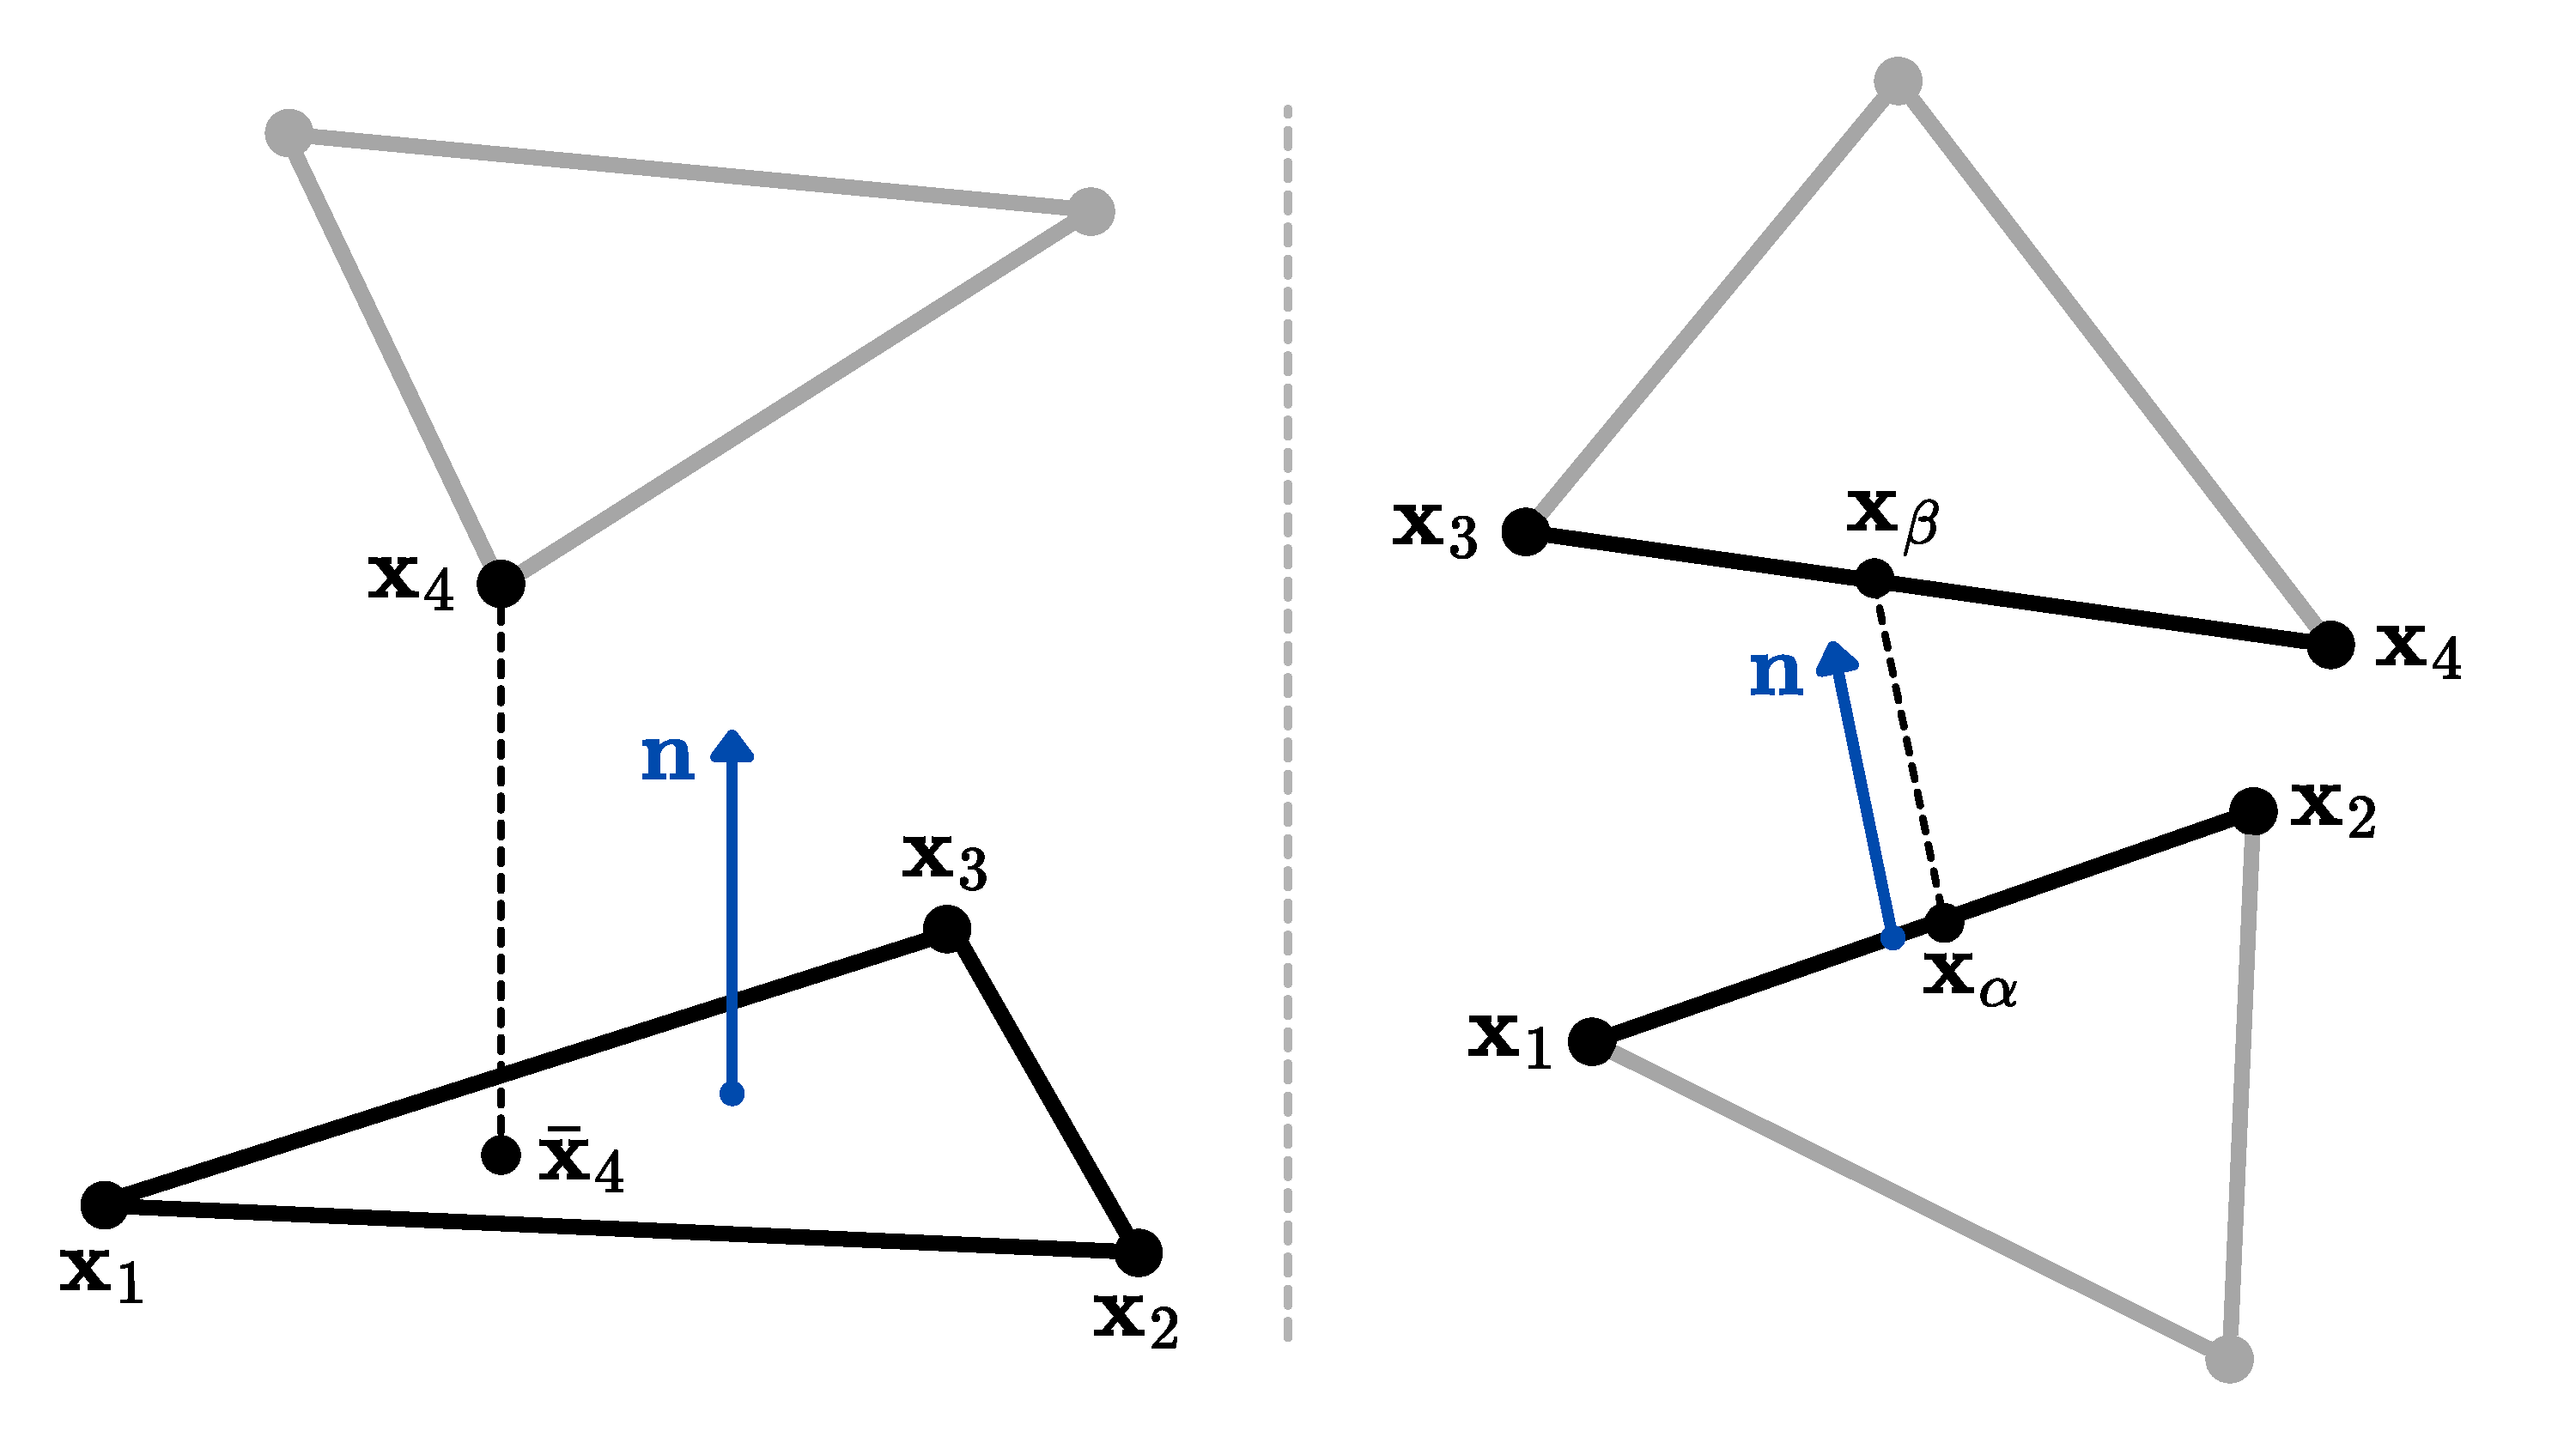
\includegraphics[width=0.95\textwidth]{images/coll_vf_ee.pdf}
\caption{The two primitive collision cases for triangle meshes: vertex-face (left) and edge-edge (right).}
\label{fig:coll_cases}
\end{figure}

For two triangle meshes, all collisions reduce to two primitive cases (Fig.~\ref{fig:coll_cases}). In both cases exactly four vertices are involved, and the signed distance between the two primitives takes the unified form:
\begin{equation}
    \delta = \bigg(\sum_{i=1}^4 w_i \mathbf{x}_i\bigg)\cdot \mathbf{n}
\end{equation}
where $\mathbf{n}$ is the collision normal and the weights $w_i$ depend on the case.

\paragraph{Vertex-Face.}
Vertices $\mathbf{x}_1, \mathbf{x}_2, \mathbf{x}_3$ form the face and $\mathbf{x}_4$ is the colliding vertex. Let $\bar{\mathbf{x}}_4 = \alpha_1\mathbf{x}_1 + \alpha_2\mathbf{x}_2 + \alpha_3\mathbf{x}_3$ be the projection of $\mathbf{x}_4$ onto the face, with $\alpha_i$ its barycentric coordinates. The signed distance is:
\begin{equation*}
\delta = 
    (\mathbf{x}_4 - \bar{\mathbf{x}}_4)\cdot \mathbf{n} =
    (\mathbf{x}_4 - \alpha_1\mathbf{x}_1 - \alpha_2\mathbf{x}_3 - \alpha_3\mathbf{x}_3)\cdot \mathbf{n}
\end{equation*}
giving weights:
\begin{equation*}
    w_1 = -\alpha_1, \qquad w_2 = -\alpha_2, \qquad w_3 = -\alpha_3, \qquad w_4 = 1
\end{equation*}
and $\mathbf{n}$ is the face normal.

\paragraph{Edge-Edge.}
Edges $(\mathbf{x}_1, \mathbf{x}_2)$ and $(\mathbf{x}_3, \mathbf{x}_4)$ have closest points $\mathbf{x}_\alpha = (1-\alpha)\mathbf{x}_1 + \alpha\mathbf{x}_2$ and $\mathbf{x}_\beta = (1-\beta)\mathbf{x}_3 + \beta\mathbf{x}_4$, with $\alpha, \beta \in [0,1]$. The signed distance is:
\begin{equation*}
\delta = 
    (\mathbf{x}_{\beta} - \mathbf{x}_{\alpha})\cdot \mathbf{n} =
    ((1 - \beta)\mathbf{x}_3 + \beta\,\mathbf{x}_4 - (1 - \alpha)\mathbf{x}_1 - \alpha\,\mathbf{x}_2)\cdot \mathbf{n}
\end{equation*}
giving weights:
\begin{equation*}
    w_1 = -(1-\alpha), \qquad w_2 = -\alpha, \qquad w_3 = (1-\beta), \qquad w_4 = \beta
\end{equation*}
and $\mathbf{n} = \frac{(\mathbf{x}_2 - \mathbf{x}_1)\times(\mathbf{x}_4 - \mathbf{x}_3)}{\|(\mathbf{x}_2 - \mathbf{x}_1)\times(\mathbf{x}_4 - \mathbf{x}_3)\|}$ is the common perpendicular to both edges.

\subsection{Collision Detection via Continuous CCD}
Assume a broad-phase algorithm (e.g. a Bounding Volume Hierarchy) has filtered out all primitive pairs that certainly do not collide during the timestep, leaving a small candidate subset. For each candidate pair, we use a Continuous Collision Detection (CCD) method to find the exact collision time within the timestep, under a linear trajectory assumption. This reduces to finding the roots of a cubic equation.

For a candidate collision pair, the positions of the involved vertices during the timestep are modeled as linear trajectories:
\begin{equation}
\label{eq:CCD_position_during_step}
    \mathbf{x}_k(t) = \mathbf{x}_k^t + t\,(\bar{\mathbf{x}}_k - \mathbf{x}_k^t)
    \qquad
    t \in [0, 1] 
    \;\;\;
    k \in [1, 2, 3, 4]
\end{equation}
where $\mathbf{x}_k^\top$ is the position at the start of the timestep and $\bar{\mathbf{x}}_k$ is the candidate position after the internal forces solve. At $t=0$ the vertex is at its original position; at $t=1$ it reaches the post-dynamics position $\bar{\mathbf{x}}_k$.

A collision occurs only when the four involved vertices become coplanar, i.e.:
\begin{equation*}
[
    (\mathbf{x}_2(t) - \mathbf{x}_1(t)) \times 
    (\mathbf{x}_3(t) - \mathbf{x}_1(t))
] \cdot (\mathbf{x}_4(t) - \mathbf{x}_1(t)) = 0
\end{equation*}
Substituting \eqref{eq:CCD_position_during_step} for each vertex, since each $\mathbf{x}_k(t)$ is linear in $t$, the scalar triple product expands to a cubic polynomial:
\begin{equation*}
a\,t^3 + b\,t^2 + c\,t + d = 0
\end{equation*}
Let $\mathcal{T}$ be the set of real roots of this equation. Roots outside $[0,1]$ are discarded (the collision does not occur within the timestep), as are roots for which the primitives do not actually intersect at time $t$ (coplanarity is necessary but not sufficient). If $\mathcal{T} = \emptyset$ the pair is collision-free; otherwise the collision time is:
\begin{equation*}
    t^* = \min(\mathcal{T})
\end{equation*}
The geometry of the involved primitives evaluated at $t^*$ (specifically the contact normal $\mathbf{n}$ and the barycentric weights $w_i$) is then used to construct the collision constraint, as described in the next section.

\begin{algorithm}[H]
\caption{Continuous Collision Detection: cubic root finding per candidate pair.}
\label{alg:CCD}
\begin{algorithmic}[1]
\addtolength{\itemsep}{0.5ex}
\Function{$\textsc{ContinuousCollisionDetection}$}{$\mathbf{x}_t, \bar{\mathbf{x}}$}
    \State $\mathbb{P} \gets \textsc{AllPossibleContactPairs}(\mathbf{x}_t, \bar{\mathbf{x}})$
    \State $\mathbb{P} \gets \textsc{BroadPhaseFiltering}(\mathbb{P})$
    \State $\mathbb{C}_{\text{oll}} \gets \emptyset$
    \For{$\mathbf{p} \in \mathbb{P}$ \textbf{in parallel}}
        \State $a, b, c, d \gets \textsc{ConstructCubicEquation}(\mathbf{p}, \mathbf{x}_t, \bar{\mathbf{x}})$
        \State $\mathcal{T} \gets \{t \in \textsc{Roots}(a,b,c,d)\mid t \in [0, 1] \wedge \textsc{IsCollision}(t, \mathbf{p}, \mathbf{x}_t, \bar{\mathbf{x}})\}$
        \If {$\mathcal{T} \neq \emptyset$}
            \State $\mathbb{C}_{\text{oll}} \gets \mathbb{C}_{\text{oll}}\;\cup\; 
            \{(\mathbf{p},\,\min(\mathcal{T}))\}$
        \EndIf
    \EndFor
    \State \Return $\mathbb{C}_{\text{oll}}$
\EndFunction
\Statex
\Function{$\textsc{IsCollision}$}{$t, \mathbf{p}, \mathbf{x}_t, \bar{\mathbf{x}}$}
    \State $\mathbf{x}_1, \mathbf{x}_2, \mathbf{x}_3, \mathbf{x}_4 \gets \textsc{InterpolatePoints}(t, \mathbf{p}, \mathbf{x}_t, \bar{\mathbf{x}})$
    \If{$\mathbf{p}$ is Vertex-Face}
        \If{$\textsc{PointIsInsideTriangle}(\mathbf{x}_4, \mathbf{x}_1, \mathbf{x}_2, \mathbf{x}_3)$}
        \State \Return True
        \EndIf
    \ElsIf{$\mathbf{p}$ is Edge-Edge}
        \If{$\textsc{SegmentsIntersect}(\mathbf{x}_1, \mathbf{x}_2, \mathbf{x}_3, \mathbf{x}_4)$}
        \State \Return True
        \EndIf
    \EndIf
    \State \Return False
\EndFunction
\end{algorithmic}
\end{algorithm}

\subsection{Collision Response as a Constrained Quadratic Problem}

Given the candidate positions $\bar{\mathbf{x}}$ produced by the dynamics step, collision response seeks the corrected positions $\mathbf{x}$ that satisfy all non-penetration constraints while deviating as little as possible from $\bar{\mathbf{x}}$. This is formulated as a constrained quadratic program:
\begin{equation}
    \min_{\mathbf{x}}\; \frac{1}{2}(\mathbf{x} - \bar{\mathbf{x}})^\top \mathbf{M}\, (\mathbf{x} - \bar{\mathbf{x}})
    \qquad 
    \text{s.t.}
    \qquad
    \mathbf{G}\mathbf{x}+\mathbf{h} \leq 0
\end{equation}
The objective is a mass-weighted displacement: heavier vertices are penalized more for moving, which is physically consistent. The constraint $\mathbf{G}\mathbf{x}+\mathbf{h} \leq 0$ encodes all $m$ detected collisions, with one row per collision pair. The construction of $\mathbf{G} \;\red{\in \mathbb{R}^{m \times 3n}}$ and $\mathbf{h} \;\red{\in \mathbb{R}^{m}}$ from the detected collisions is detailed below.

\begin{derivation}
For each primitive detected collision $j$, we require the signed distance $\delta_j$ to exceed the cloth thickness $d$:
\begin{equation*}
    \delta_j = \bigg(\sum_{i=1}^4 w_i \mathbf{x}_i\bigg)\cdot \mathbf{n}_j \ge d
\end{equation*}
Since $\delta_j$ is linear in $\mathbf{x}$, this can be written as $\mathbf{g}_j^\top\mathbf{x} \ge d$, where $\mathbf{g}_j \;\red{\in \mathbb{R}^{3n}}$ is sparse, with nonzero entries only at the 12 coordinates of the 4 involved vertices:
\begin{equation*}
\mathbf{g}_j = 
[\,\cdots\; \mathbf{0} \;\cdots\;
\underbrace{w_{j1}\,\mathbf{n}_j}_{\red{\in\,\mathbb{R}^3}}
\;\cdots\; \mathbf{0} \;\cdots\;
\underbrace{w_{j2}\,\mathbf{n}_j}_{\red{\in\,\mathbb{R}^3}}
\;\cdots\; \mathbf{0} \;\cdots\,]
\end{equation*}
Rewriting in the standard form $c \leq 0$ gives $-\mathbf{g}_j^\top\mathbf{x} + d \leq 0$. Stacking all $m$ collision constraints yields:
\begin{equation*}
\mathbf{G} = 
\begin{bmatrix}
    -\mathbf{g}_1^\top \\[0.5ex]
    -\mathbf{g}_2^\top \\[0.5ex]
    \vdots          \\[0.5ex]
    -\mathbf{g}_m^\top \\[0.5ex]
\end{bmatrix} 
\red{\in \mathbb{R}^{m\times 3n}}
\qquad
\mathbf{h} = 
\begin{bmatrix}
    d      \\[0.5ex]
    d      \\[0.5ex]
    \vdots \\[0.5ex]
    d      \\[0.5ex]
\end{bmatrix} 
\red{\in \mathbb{R}^{m}}
\end{equation*}
\end{derivation}

\begin{figure}[htbp]
\centering
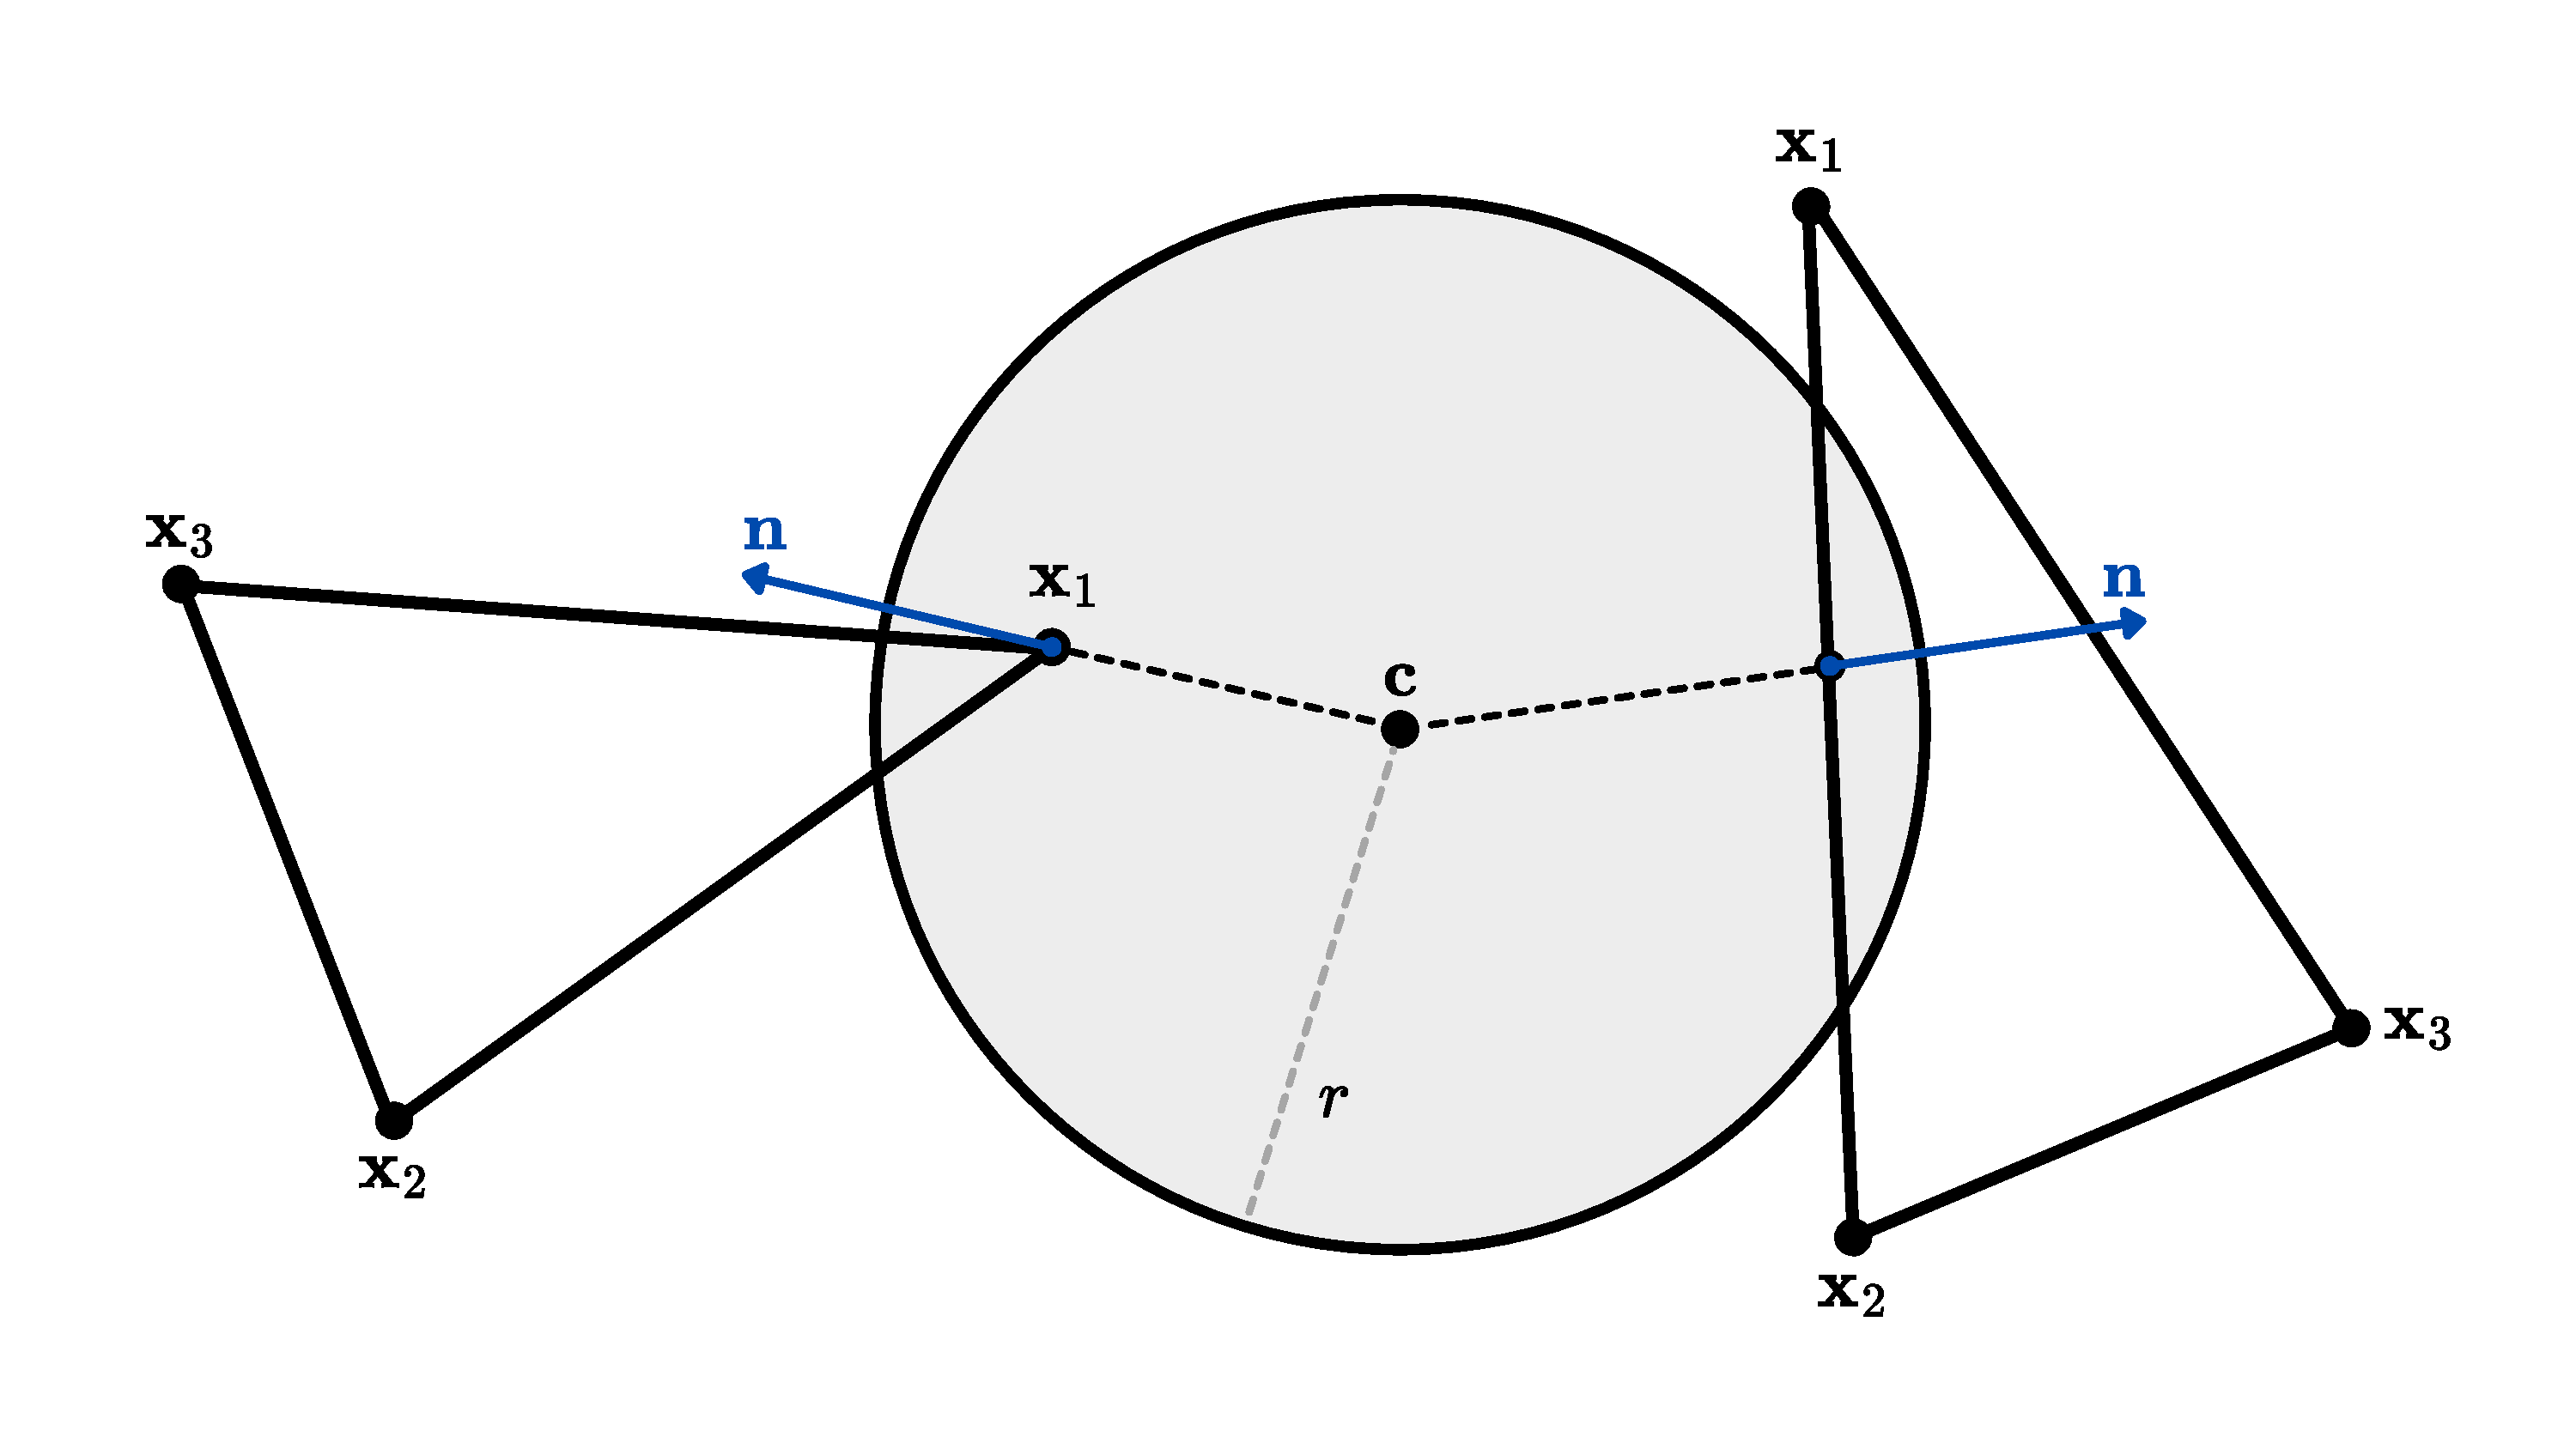
\includegraphics[width=0.95\textwidth]{images/triangle_sphere_coll.pdf}
\caption{}
\label{fig:coll_cases}
\end{figure}
\paragraph{Face-Sphere.}
Let $\mathbf{x}_1, \mathbf{x}_2, \mathbf{x}_3$ be the triangle vertices, $\mathbf{c} \in \mathbb{R}^3$ the sphere center, and $r$ its radius. The contact point is the closest point on the triangle to $\mathbf{c}$:
\begin{equation*}
    \bar{\mathbf{x}} = \alpha_1\mathbf{x}_1 + \alpha_2\mathbf{x}_2 + \alpha_3\mathbf{x}_3
\end{equation*}
where $\alpha_i$ are the barycentric coordinates of the projection of $\mathbf{c}$ onto the triangle, clamped to lie within it. The outward contact normal is $\mathbf{n} = \frac{\bar{\mathbf{x}} - \mathbf{c}}{\|\bar{\mathbf{x}} - \mathbf{c}\|}$ and the signed distance is:
\begin{equation*}
    \delta = (\bar{\mathbf{x}} - \mathbf{c}) \cdot \mathbf{n}
\end{equation*}
\begin{derivation}
The constraint $\delta \geq r$ reads $\mathbf{g}^\top\mathbf{x} \geq d$ with:
\begin{equation*}
    \mathbf{g} = [\,\cdots\;\mathbf{0}\;\cdots\;
    \underbrace{\alpha_1\mathbf{n}}_{\red{\in\,\mathbb{R}^3}}\;\cdots\;
    \underbrace{\alpha_2\mathbf{n}}_{\red{\in\,\mathbb{R}^3}}\;\cdots\;
    \underbrace{\alpha_3\mathbf{n}}_{\red{\in\,\mathbb{R}^3}}\;\cdots\;\mathbf{0}\;\cdots\,]
    \qquad
    d = r + \mathbf{c}\cdot\mathbf{n}
\end{equation*}
where the nonzero entries correspond to the 9 coordinates of $\mathbf{x}_1, \mathbf{x}_2, \mathbf{x}_3$. The sphere contributes no degrees of freedom.
\end{derivation}


\subsubsection{Solution via Non-Rigid Impact Zones}
We now present an approximate solution to the collision response QP, adapting the non-rigid impact zone method of \cite{harmon2008robust} to position space. The approximation consists of relaxing the inequality constraints to equalities, requiring each signed distance to be exactly at the thickness boundary rather than above it:
\begin{equation}
    \min_{\mathbf{x}}\; \frac{1}{2}(\mathbf{x} - \bar{\mathbf{x}})^\top \mathbf{M}\, (\mathbf{x} - \bar{\mathbf{x}})
    \qquad 
    \text{s.t.}
    \qquad
    \mathbf{G}\mathbf{x}+\mathbf{h}\; \red{=}\; 0
\end{equation}
This relaxation may produce negative Lagrange multipliers, introducing mild artificial sticking (since constraints may be pulled rather than pushed), but reduces the problem to a simple linear solve. The Lagrangian is:
\begin{equation*}
\mathcal{L}(\mathbf{x}, \lambda) = 
    \frac{1}{2}(\mathbf{x} - \bar{\mathbf{x}})^\top \mathbf{M}\, (\mathbf{x} - \bar{\mathbf{x}}) + 
    (\mathbf{G}\mathbf{x}+\mathbf{h})^\top\lambda
\end{equation*}
The stationarity condition $\pdc{\mathcal{L}}{\mathbf{x}} = 0$ gives:
\begin{equation}
\label{eq:nonrigid_impact_position_solution}
\mathbf{x}^* = \bar{\mathbf{x}} - \mathbf{M}^{-1}\mathbf{G}^\top\lambda
\end{equation}
Substituting into the equality constraint $\mathbf{G}\mathbf{x}^* + \mathbf{h} = 0$ yields a linear system for the multipliers:
\begin{equation}
\label{eq:nonrigid_impact_linear_system}
    \underbrace{[\mathbf{G}\mathbf{M}^{-1}\mathbf{G}^\top]}_{\mathbf{A}\;\red{\in\;\mathbb{R}^{m\times m}}}\;\lambda = \underbrace{\mathbf{G}\bar{\mathbf{x}} + \mathbf{h}}_{\mathbf{b}\;\red{\in\;\mathbb{R}^{m}}}
\end{equation}
Solving for $\lambda$ and substituting back into \eqref{eq:nonrigid_impact_position_solution} yields the corrected positions $\mathbf{x}^*$ satisfying all constraints.

\paragraph{Impact Zone Decomposition} Since $\mathbf{A}_{ij} = \mathbf{g}_i^\top \mathbf{M}^{-1} \mathbf{g}_j = 0$ whenever constraints $i$ and $j$ share no vertices, $\mathbf{A}$ is block-diagonal when constraints are sorted by impact zone. Each impact zone $k$, involving $m_k$ constraints and $n_k$ vertices, yields one independent block system:
\begin{equation*}
    \mathbf{A}^{k}\lambda^{k} = \mathbf{b}^{k}
\end{equation*}
\begin{equation*}
    \mathbf{A}^{k} = \mathbf{G}^{k}(\mathbf{M}^{k})^{-1}(\mathbf{G}^{k})^\top \;\red{\in \mathbb{R}^{m_k \times m_k}}
    \qquad
    \mathbf{b}^{k} = \mathbf{G}^{k}\bar{\mathbf{x}}^{k} + \mathbf{h}^{k} \;\red{\in \mathbb{R}^{m_k}}
\end{equation*}
where all quantities are restricted to the $n_k$ vertices of zone $k$. Since the blocks are independent, each system can be assembled and solved in parallel. 

\begin{definitionbox}[frametitle={Impact Zone}]
Define the constraint graph $\mathcal{G} = (\mathcal{V}, \mathcal{E})$, where each node $i \in \mathcal{V}$ corresponds to a collision constraint, and an edge $(i,j) \in \mathcal{E}$ exists if and only if constraints $i$ and $j$ share at least one vertex in their stencil. An \textbf{impact zone}, then, is a connected component of $\mathcal{G}$.
\end{definitionbox}

\begin{algorithm}[H]
\caption{Non-Rigid Impact Zone collision response (single-iteration approximation).}
\label{alg:nonrigid_impact_zone}
\begin{algorithmic}[1]
\addtolength{\itemsep}{0.5ex}
\Function{$\textsc{NonRigidImpactZoneCollisionResponse}$}{$\mathbf{x}_t, \bar{\mathbf{x}}, \mathbf{M}, d$}
    \State $\mathbb{C}_{\text{oll}} \gets \textsc{CCD}(\mathbf{x}_t, \bar{\mathbf{x}})$
    \State $\mathbf{G}, \mathbf{h} \gets \textsc{ConstructConstraints}(\mathbb{C}_{\text{oll}}, \mathbf{x}_t, \bar{\mathbf{x}}, d)$
    \State $\mathbf{x}^* \gets \bar{\mathbf{x}}$
    \State $\mathbb{I}_\text{z} \gets \textsc{GroupByImpactZones}(\mathbf{G}, \mathbf{h})$
    \For{$Z \in \mathbb{I}_\text{z}$ \textbf{in parallel}}
        \State $\mathbf{x}^* \gets \textsc{ApplyProjection}(Z, \bar{\mathbf{x}}, \mathbf{M})$ \graycomment{Eqs.~\ref{eq:nonrigid_impact_linear_system},~\ref{eq:nonrigid_impact_position_solution}}
    \EndFor
    \State \Return $\mathbf{x}^*$
\EndFunction
\end{algorithmic}
\end{algorithm}

\newpage

\section{Implicit Differentiation}
\label{sec:implicit_diff}

Given that we already know $\pdc{\phi}{\mathbf{y}}$, we want to calculate $\pdc{\phi}{\mathbf{u}}$. We have a system of implicit constraints:
\begin{equation*}
    \mathbf{F}(\mathbf{y}, \mathbf{u}) = \mathbf{0}
\end{equation*}
that binds $\mathbf{y}$ and $\mathbf{u}$ together, where $\mathbf{y}\;\red{\in \mathbb{R}^{n}}$ is considered the output, $\mathbf{u}\;\red{\in \mathbb{R}^{m}}$ the input and $\mathbf{F}:\;\red{\mathbb{R}^{n}  \times \mathbb{R}^{m} \rightarrow \mathbb{R}^{l}}$ .
\newline First, we totally differentiate the constraint $\mathbf{F} = 0$:
\begin{equation}
    \pd{\mathbf{F}}{\mathbf{y}}d\mathbf{y} + \pd{\mathbf{F}}{\mathbf{u}}d\mathbf{u} = 0
\end{equation}
solving for $d\mathbf{y}$:
\begin{equation*}
    d\mathbf{y} = 
    - \left(\pd{\mathbf{F}}{\mathbf{y}}\right)^{-1}\pd{\mathbf{F}}{\mathbf{u}}d\mathbf{u} = 
    -\mathbf{J}^{-1}\pd{\mathbf{F}}{\mathbf{u}}d\mathbf{u}
\end{equation*}
where $\mathbf{J} = \pdc{\mathbf{F}}{\mathbf{y}}\;\red{\in \mathbb{R}^{l\times n}}$ is the Jacobian of the constraint with respect to the output. Then, the loss change with respect to $d\mathbf{u}$ is:
\begin{equation*}
d\phi = 
    \left(\pd{\phi}{\mathbf{y}}\right)^\top d\mathbf{y} = 
    - \left(\pd{\phi}{\mathbf{y}}\right)^\top \mathbf{J}^{-1}\pd{\mathbf{F}}{\mathbf{u}}d\mathbf{u}
\end{equation*}
We define the adjoint vector $\boldsymbol{\mu}$ as:
\begin{equation}
\boldsymbol{\mu} = \mathbf{J}^{-T} \pd{\phi}{\mathbf{y}}
\qquad
\Longrightarrow
\qquad
\mathbf{J}^\top \boldsymbol{\mu} = \pd{\phi}{\mathbf{y}}
\end{equation}
which can be found by solving the linear system on the right. 
\newline Then the gradient loss can be re-written as:
\begin{equation*}
d\phi = -\boldsymbol{\mu}^\top \pd{\mathbf{F}}{\mathbf{u}} d\mathbf{u}
\end{equation*}
that let us calculate the gradient of the loss with respect to $\mathbf{u}$:
\begin{equation}
    \pd{\phi}{\mathbf{u}} = - \left( \pd{\mathbf{F}}{\mathbf{u}} \right)^\top \boldsymbol{\mu}
\end{equation}

\subsection{Linear Solve}

\begin{figure}
    \centering
    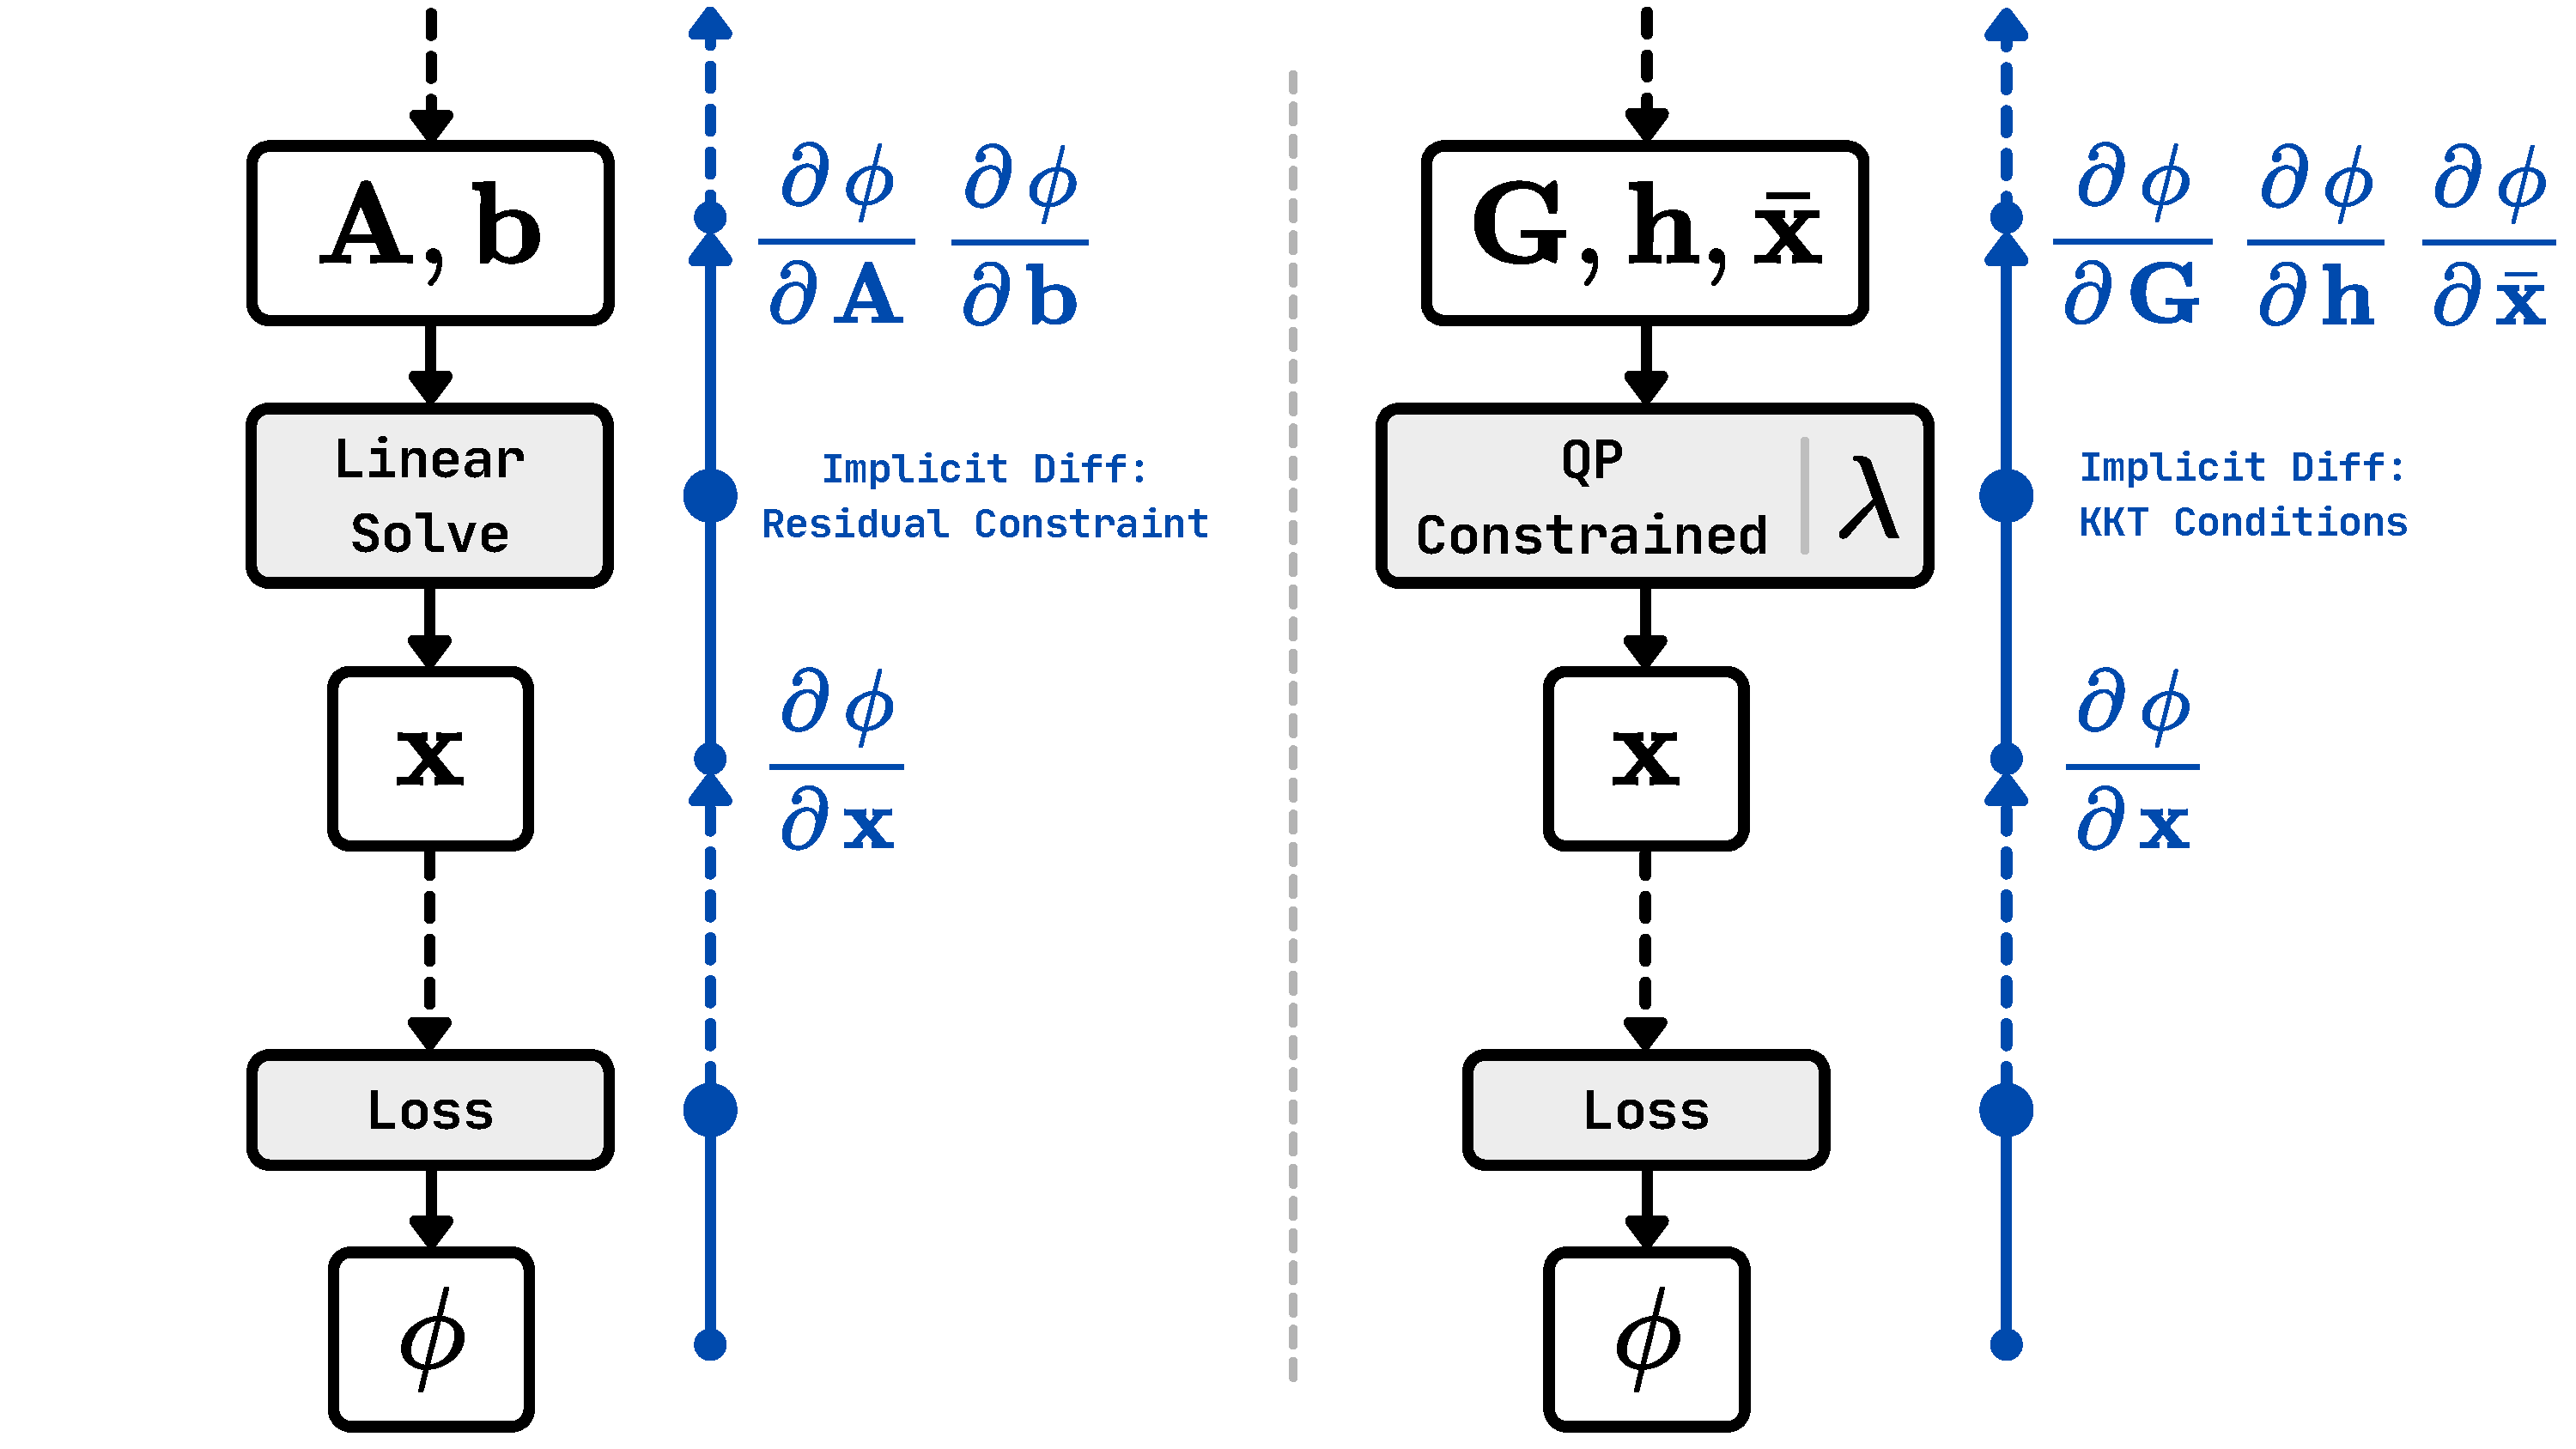
\includegraphics[width=0.95\textwidth, trim={0cm 0 0cm 0}, clip]{images/impl_diff_pipeline.pdf}
    \caption{Forward and backward pipeline...}
    \label{fig:implicit_diff_pipeline}
\end{figure}

During the forward pass, the simulation requires solving the linear system
\begin{equation*}
    \mathbf{A}\mathbf{x} = \mathbf{b}
    \qquad 
    \text{with } 
    \mathbf{A} \red{\;\in \mathbb{R}^{3n\times 3n}}, 
    \; \mathbf{b}\red{\;\in \mathbb{R}^{3n}}
\end{equation*}
for the unknown $\mathbf{x}$. During the backward pass, given the upstream gradient $\partial\phi/\partial\mathbf{x}$, we seek $\partial\phi/\partial\mathbf{A}$ and $\partial\phi/\partial\mathbf{b}$. We first solve the linear system
\begin{equation}
    \mathbf{A}^\top \boldsymbol{\mu} = \frac{\partial \phi}{\partial \mathbf{x}}
\end{equation}
to find the adjoint vector $\boldsymbol{\mu} \red{\; \in \mathbb{R}^{3n}}$, from which the gradients follow as:
\begin{equation}
\label{eq:impdiff_gradA_gradb}
    \frac{\partial\phi}{\partial\mathbf{b}} = \boldsymbol{\mu} 
    \red{\; \in \mathbb{R}^{3n}}
    \qquad
    \frac{\partial\phi}{\partial\mathbf{A}} = -\boldsymbol{\mu}\,\mathbf{x}^\top
    \red{\; \in \mathbb{R}^{3n\times 3n}}
\end{equation}

\begin{derivation}
Following the method presented in Section \ref{sec:implicit_diff}, the linear system defines the implicit residual constraint:
\begin{equation*}
    \mathbf{F}(\mathbf{x}, \mathbf{A}, \mathbf{b}) = \mathbf{A}\mathbf{x} - \mathbf{b} = \mathbf{0}
\end{equation*}
with output $\mathbf{y} = \mathbf{x}$ and inputs $\mathbf{u} = (\mathbf{A}, \mathbf{b})$.
The Jacobian with respect to the output is:
\begin{equation*}
    \mathbf{J} = \pd{\mathbf{F}}{\mathbf{x}} = \mathbf{A}
\end{equation*}
so the adjoint system $\mathbf{J}^\top\boldsymbol{\mu} = \pdc{\phi}{\mathbf{x}}$ becomes:
\begin{equation*}
    \mathbf{A}^\top\boldsymbol{\mu} = \pd{\phi}{\mathbf{x}}.
\end{equation*}
The gradients then follow from $\pdc{\phi}{\mathbf{u}} = -(\pdc{\mathbf{F}}{\mathbf{u}})^\top\boldsymbol{\mu}$.
Computing: 
\begin{equation*}
\pd{\mathbf{F}}{\mathbf{b}} = -\mathbf{I} 
\qquad\qquad
\pd{\mathbf{F}}{\mathbf{A}} = \mathbf{x}^\top 
\end{equation*}
gives:
\begin{equation*}
    \pd{\phi}{\mathbf{b}} = -(-\mathbf{I})^\top\boldsymbol{\mu} = \boldsymbol{\mu}
    \qquad
    \pd{\phi}{\mathbf{A}} = -\mathbf{x}\boldsymbol{\mu}^\top = -\boldsymbol{\mu}\,\mathbf{x}^\top,
\end{equation*}
which recovers \eqref{eq:impdiff_gradA_gradb}.
\end{derivation}

\subsection{Quadratic Program with only Linear Inequality Constraints}
Here we follow derivations of the Paper \cite{liang2019differentiable}. During the forward pass, the simulation might solves the constrained QP
\begin{equation*}
    \min_{\mathbf{x}}\; \frac{1}{2}(\mathbf{x} - \bar{\mathbf{x}})^\top \mathbf{M}\, (\mathbf{x} - \bar{\mathbf{x}})
    \qquad 
    \text{s.t.}
    \qquad
    \mathbf{G}\mathbf{x}+\mathbf{h} \leq 0,
\end{equation*}
During the backward pass, given $\pdc{\phi}{\mathbf{x}}$, we seek $\pdc{\phi}{\mathbf{G}}$, $\pdc{\phi}{\mathbf{h}}$, and $\pdc{\phi}{\bar{\mathbf{x}}}$.

\noindent Following the general implicit differentiation framework of Section~\ref{sec:implicit_diff}, we use the KKT stationarity and complementary slackness conditions as the implicit constraints $\mathbf{F} = \mathbf{0}$. Identifying the Jacobian $\mathbf{J} = \pdc{\mathbf{F}}{[\mathbf{x}, \lambda]}$ and applying $\mathbf{J}^\top\boldsymbol{\mu} = \pdc{\phi}{[\mathbf{x}, \lambda]}$ yields the linear system:
\begin{equation}
\label{eq:impl_diff_QP_lin_system}
    \begin{bmatrix}
        \;\mathbf{M} & \mathbf{G}^\top\, \textsc{Diag}(\lambda)\;\\[2ex]
        \;\mathbf{G} & \textsc{Diag}(\mathbf{G}\mathbf{x}+\mathbf{h})\;
    \end{bmatrix}
    \begin{bmatrix}
        \mathbf{d}_\mathbf{x} \\[2ex]
        \mathbf{d}_\lambda
    \end{bmatrix} = 
    \begin{bmatrix}
        \left(\pdc{\phi}{\mathbf{x}}\right)^\top\\[2ex]
        \mathbf{0}
    \end{bmatrix}
\end{equation}
where the zero in the right-hand side reflects that $\lambda$ does not appear in the loss directly.
From the solution $(\mathbf{d}_\mathbf{x}, \mathbf{d}_\lambda)$, the gradients follow as
\begin{align}
    \pd{\phi}{\bar{\mathbf{x}}} &= 
        \mathbf{d}_\mathbf{x}^\top\mathbf{M} 
         &&\red{\in \mathbb{R}^{3n}} \\[1ex]
    \pd{\phi}{\mathbf{G}} &= 
        -\textsc{Diag}(\lambda)\,\mathbf{d}_\lambda\,\mathbf{x}^{\top} - \lambda\,\mathbf{d}_\mathbf{x}^\top 
        &&\red{\in \mathbb{R}^{m\times 3n}} \\[1ex]
    \pd{\phi}{\mathbf{h}} &= 
        -\mathbf{d}_\lambda^\top\,\textsc{Diag}(\lambda)
        &&\red{\in \mathbb{R}^m}
\end{align}
The linear system~\ref{eq:impl_diff_QP_lin_system} is expensive to solve directly. Assuming all constraints are perfectly satisfied, i.e. $\mathbf{G}\mathbf{x}+\mathbf{h} = \mathbf{0}$, the bottom-right block of the system vanishes and the adjoint vectors can instead be obtained in closed form. We first compute the QR decomposition
\begin{equation}
    \sqrt{\mathbf{M}}^{-1}\mathbf{G}^\top = \mathbf{Q}\mathbf{R}
\end{equation}
from which the adjoint vectors follow directly as
\begin{align}
\mathbf{d}_\mathbf{x} &= 
    \sqrt{\mathbf{M}}^{-1}(\mathbf{I} - 
    \mathbf{Q}\mathbf{Q}^\top)\sqrt{\mathbf{M}}^{-1}
    \left(\pd{\phi}{\mathbf{x}}\right)^\top
\\[1ex]
\mathbf{d}_\lambda &=
    \textsc{Diag}(\lambda)^{-1}\mathbf{R}^{-1}\mathbf{Q}^\top\sqrt{\mathbf{M}}^{-1}\left(\pd{\phi}{\mathbf{x}}\right)^\top
\end{align}

\subsection{Generic Constrained Quadratic Program}
Here we follow the derivations of \cite{amos2017optnet}. Given the constrained QP:
\begin{gather*}
    \min_\mathbf{x}\; \frac{1}{2}\mathbf{x}^\top \mathbf{Q}\,\mathbf{x} + \mathbf{q}^\top \mathbf{x} 
    \qquad \text{such that} \\
    \mathbf{A}\,\mathbf{x}\, =    \,\mathbf{b} \\
    \mathbf{G}\,\mathbf{x}\, \leq \,\mathbf{h}
\end{gather*}
and given $\pdc{\phi}{\mathbf{x}^\star}$, we seek $\pdc{\phi}{\mathbf{Q}}, \pdc{\phi}{\mathbf{q}}, \pdc{\phi}{\mathbf{A}}, \pdc{\phi}{\mathbf{b}}, \pdc{\phi}{\mathbf{G}}, \pdc{\phi}{\mathbf{h}}$.

\noindent The Lagrangian of the problem is:
\begin{equation*}
\mathcal{L}(\mathbf{x}, \nu, \lambda) = 
    \frac{1}{2}\mathbf{x}^\top \mathbf{Q}\,\mathbf{x} + \mathbf{q}^\top \mathbf{x} +
    \nu^\top(\mathbf{A}\mathbf{x}-\mathbf{b}) +
    \lambda^\top(\mathbf{G}\mathbf{x} - \mathbf{h})
\end{equation*}
The KKT stationary, primal feasibility, and complementary slackness conditions at the optimal $(\mathbf{x}^\star, \nu^\star, \lambda^\star)$ are:
\begin{equation*}
\mathbf{F}(\mathbf{x}^\star, \nu^\star, \lambda^\star) = \begin{cases}
    \mathbf{Q}\,\mathbf{x}^\star + \mathbf{q} + \mathbf{A}^\top \nu^\star + \mathbf{G}^\top \lambda^\star = \mathbf{0} \\[0.5ex]
    \mathbf{A}\,\mathbf{x}^\star - \mathbf{b} = \mathbf{0} \\[0.5ex]
    \textsc{Diag}(\lambda^\star)(\mathbf{G}\mathbf{x}^\star-\mathbf{h}) = \mathbf{0}
\end{cases}
\end{equation*}
We treat these as the implicit constraint $\mathbf{F} = \mathbf{0}$ of Section~\ref{sec:implicit_diff}, with output $\mathbf{y} = (\mathbf{x}^\star, \nu^\star, \lambda^\star)$ and inputs $\mathbf{u} = (\mathbf{Q}, \mathbf{q}, \mathbf{A}, \mathbf{b}, \mathbf{G}, \mathbf{h})$. The adjoint system $\mathbf{J}^\top \boldsymbol{\mu} = \pdc{\phi}{\mathbf{y}}$ becomes:
\begin{equation}
\label{eq:optnet_adjoint}
\begin{bmatrix}
    \mathbf{Q} & \mathbf{G}^\top\textsc{Diag}(\lambda^\star) & \mathbf{A}^\top \\[1ex]
    \mathbf{G} & \textsc{Diag}(\mathbf{G}\mathbf{x}^\star - \mathbf{h}) & \mathbf{0} \\[1ex]
    \mathbf{A} & \mathbf{0} & \mathbf{0}
\end{bmatrix}
\begin{bmatrix}
    \mathbf{d}_\mathbf{x} \\[1ex] \mathbf{d}_{\lambda} \\[1ex] \mathbf{d}_{\nu}
\end{bmatrix}
=
\begin{bmatrix}
    \left(\pdc{\phi}{\mathbf{x}^\star}\right)^\top \\[1ex] \mathbf{0} \\[1ex] \mathbf{0}
\end{bmatrix}
\end{equation}
where the zeros on the right reflect that the loss does not depend directly on $\lambda^\star$ or $\nu^\star$. From the solution $(\mathbf{d}_\mathbf{x}, \mathbf{d}_\lambda, \mathbf{d}_\nu)$, the parameter gradients follow as:
\begin{equation}
\label{eq:optnet_gradients}
\begin{aligned}
    \pd{\phi}{\mathbf{Q}} &= \frac{1}{2}(\mathbf{d}_\mathbf{x}\,\mathbf{x}^{\star\top} + \mathbf{x}^\star\mathbf{d}_\mathbf{x}^\top) 
    &\qquad
    \pd{\phi}{\mathbf{q}} &= \mathbf{d}_\mathbf{x} \\[1ex]
    \pd{\phi}{\mathbf{A}} &= \mathbf{d}_\nu\,\mathbf{x}^{\star\top} + \nu^\star\mathbf{d}_\mathbf{x}^\top 
    &\qquad
    \pd{\phi}{\mathbf{b}} &= -\mathbf{d}_\nu \\[1ex]
    \pd{\phi}{\mathbf{G}} &= \textsc{Diag}(\lambda^\star)\,\mathbf{d}_\lambda\,\mathbf{x}^{\star\top} + \lambda^\star\mathbf{d}_\mathbf{x}^\top 
    &\qquad
    \pd{\phi}{\mathbf{h}} &= -\textsc{Diag}(\lambda^\star)\,\mathbf{d}_\lambda
\end{aligned}
\end{equation}

\subsection{Linear Complementary Problem}
Given the LCP:
\begin{align*}
    \text{find } \mathbf{x} \in \mathbb{R}^n \text{ such that: } \\
    &&\mathbf{M}\mathbf{x} + \mathbf{q} &\ge 0 \\
    &&\mathbf{x} &\ge 0 \\
    &&\mathbf{x}^\top(\mathbf{M}\mathbf{x} + \mathbf{q}) &= 0 \\
\end{align*}
and given $\pdc{\phi}{\mathbf{x}^\star}$, we seek $\pdc{\phi}{\mathbf{M}}, \pdc{\phi}{\mathbf{q}}$.

\noindent We introduce the slack variable $\mathbf{w} = \mathbf{M}\mathbf{x} + \mathbf{q}$ and define the two implicit constraints:
\begin{align*}
    &\mathbf{F}_1(\mathbf{x}^\star, \mathbf{w}^\star, \mathbf{M}, \mathbf{q}) = \mathbf{M}\mathbf{x}^\star + \mathbf{q} - \mathbf{w}^\star = 0\\
    &\mathbf{F}_2(\mathbf{x}^\star, \mathbf{w}^\star) = \textsc{Diag}(\mathbf{x}^\star)\mathbf{w}^\star =0 
\end{align*}
Then $\mathbf{J}$ is:
\begin{equation}
\pd{\mathbf{F}}{[\mathbf{x}^\star, \mathbf{w}^\star]} = \mathbf{J} = 
\begin{bmatrix}
    \;\mathbf{M} & -\mathbf{I}\; \\
    \;\textsc{Diag}(\mathbf{w}^\star) & \textsc{Diag}(\mathbf{x}^\star)\;
\end{bmatrix}
\end{equation}
The adjoint vector is obtained by solving the linear system:
\begin{equation}
\begin{bmatrix}
    \;\mathbf{M}^\top & \textsc{Diag}(\mathbf{w}^\star)\; \\
    \;-\mathbf{I} & \textsc{Diag}(\mathbf{x}^\star)\;
\end{bmatrix}
\begin{bmatrix}
    \mathbf{d}_\mathbf{x} \\
    \mathbf{d}_\mathbf{w}
\end{bmatrix} = 
\begin{bmatrix}
    (\pdc{\phi}{\mathbf{x}^\star})^\top \\
    0
\end{bmatrix}
\end{equation}
And the gradients with resoect to the input are:
\begin{equation}
    \pd{\phi}{\mathbf{M}} = -\mathbf{d}_\mathbf{x} {\mathbf{x}^\star}^\top
    \qquad
    \pd{\phi}{\mathbf{q}} = -\mathbf{d}_\mathbf{x}
\end{equation}

\newpage

\section{Differentiable Cloth Simulation for Inverse Problems \cite{liang2019differentiable}}
\label{sec:DiffCloth}

Building on Sections \ref{sec:collisions} and \ref{sec:implicit_diff} we will build a forward and backward simulation methodology very similar to the one proposed in the Paper \cite{liang2019differentiable}. 

\begin{algorithm}[H]
\caption{}
\label{alg:diff_cloth_like_sim_algo}
\begin{algorithmic}[1]
\addtolength{\itemsep}{0.5ex}
\Function{$\textsc{}$}{$\mathbf{x}^-, \mathbf{v}^-, \mathbf{M}, h$}
    \State $\mathbf{\hat{M}}, \mathbf{\hat{f}} \gets \textsc{BuildLinearSystem}(\mathbf{x}^-, \mathbf{v}^-, \mathbf{M}, h)$ 
    \graycomment{Eq.~\ref{eq:implicit_sim_position_based}}
    \State $\textsc{Solve }\;\mathbf{\hat{M}}\Delta \mathbf{x}  =  \mathbf{\hat{f}}$
    \State $\bar{\mathbf{x}} \gets \mathbf{x}^- + \Delta \mathbf{x}$
    \State $\mathbf{G}, \mathbf{h} \gets \textsc{CCD}(\mathbf{x}^-, \bar{\mathbf{x}})$
    \graycomment{Algo.~\ref{alg:CCD}}
    \State $\mathbf{x}^+ \gets \textsc{SolveQP}(\bar{\mathbf{x}},  \mathbf{M}, \mathbf{G}, \mathbf{h})$
    \graycomment{Algo.~\ref{alg:nonrigid_impact_zone}}
    \State $\mathbf{v}^+ \gets \frac{1}{h}(\mathbf{x}^+ - \mathbf{x}^-)$
\EndFunction
\end{algorithmic}
\end{algorithm}

\newpage

\newcommand{\RR}{\mathbb{R}}
\newcommand{\x}{\mathbf{x}}
\newcommand{\vv}{\mathbf{v}}
\newcommand{\q}{\mathbf{q}}
\newcommand{\f}{\mathbf{f}}
\newcommand{\g}{\mathbf{g}}
\newcommand{\A}{\mathbf{A}}
\newcommand{\J}{\mathbf{J}}
\newcommand{\bb}{\mathbf{b}}
\newcommand{\M}{\mathbf{M}}
\newcommand{\C}{\mathbf{C}}
\newcommand{\F}{\mathbf{F}}
\newcommand{\R}{\mathbf{R}}
\newcommand{\I}{\mathbf{I}}
\newcommand{\zero}{\mathbf{0}}
\newcommand{\z}{\mathbf{z}}
\newcommand{\e}{\mathbf{e}}
\newcommand{\p}{\mathbf{p}}
\newcommand{\dd}{\mathbf{d}}
\newcommand{\G}{\mathbf{G}}
\newcommand{\rr}{\mathbf{r}}
\newcommand{\tb}{\mathbf{t}}
\newcommand{\Sb}{\mathbf{S}}
\newcommand{\B}{\mathbf{B}}
\newcommand{\LL}{\mathbf{L}}
\newcommand{\n}{\mathbf{n}}

\section{Projective Dynamics (PD) \cite{bouaziz2023projective}}
\label{sec:pd}

We start with the variational form of implicit Euler integration. Given the current state, the inertial estimate $\tilde{\x} = \x^- + h\vv^- + h^2\M^{-1}\f_{\text{ext}}$ predicts where each vertex would land under momentum and external forces alone. The next positions $\x^+$ balance this inertial trajectory against elastic resistance:
\begin{equation}
\label{eq:PD_variational_form}
\x^+ = \arg \min_{\x} 
    \underbrace{\frac{1}{2h^2}(\x - \tilde{\x})^\top\M\,(\x - \tilde{\x})}_{\text{momentum potential}} + 
    \underbrace{\sum_i\;U_i(\x)}_{\text{elastic potential}}
\end{equation}
The momentum potential penalizes deviation from the inertial trajectory, weighted by mass. The elastic potential penalizes deformation away from the rest configuration. Their balance determines the motion.

\subsection{Constraint-Based Energy Potentials}

The key idea of Projective Dynamics is to replace each elastic potential $U_i(\x)$ with an augmented form involving an auxiliary variable $\p_i$:
\begin{equation}
    U_i(\x, \p_i) = \frac{k_i}{2} \|\A_i\Sb_i\x - \B_i\p_i\|^2_F + \delta_i(\p_i)
\end{equation}
where $\Sb_i$ is a constant selection matrix extracting the vertices involved in constraint $i$ from the global position vector $\x$, the matrices $\A_i$ and $\B_i$ are constant differential operators determined by the rest configuration (encoding, e.g., the discrete gradient operator and rest edge geometry), $k_i$ is the constraint stiffness, and:
\begin{equation}
    \delta_i(\p_i) = 
    \begin{cases}
        0 & \text{if } \p_i \in \mathcal{M}_i \\[1ex]
        +\infty & \text{otherwise}
    \end{cases}
\end{equation}
is an indicator function that forces $\p_i$ to lie on the constraint manifold $\mathcal{M}_i$, the set of admissible configurations. The distance $\|\A_i\Sb_i\x - \B_i\p_i\|^2_F$ is \emph{quadratic} in both $\x$ and $\p_i$, while all geometric nonlinearity is captured by the projection onto $\mathcal{M}_i$.
\newline Minimizing over $\p_i$ recovers the original elastic potential: $U_i(\x) = \min_{\p_i} U_i(\x, \p_i)$.

\subsection{The Augmented Problem}

Substituting the constraint-based potentials, the full problem becomes:
\begin{equation}
\min_{\x, \p} 
    \frac{1}{2h^2}(\x - \tilde{\x})^\top\M\,(\x - \tilde{\x}) + 
    \sum_i\;\frac{k_i}{2} \|\A_i\Sb_i\x - \B_i\p_i\|^2_F + \delta_i(\p_i)
\end{equation}
This is minimized via alternating optimization (block coordinate descent) over $\p$ and $\x$:

\paragraph{Local Step.} Fix $\x$, minimize over each $\p_i$ independently:
\begin{equation}
    \p_i^* = \arg\min_{\p_i \in \mathcal{M}_i} \frac{k_i}{2} \|\A_i\Sb_i\x - \B_i\p_i\|^2_F
\end{equation}
This is a projection of $\A_i\Sb_i\x$ onto the constraint manifold $\mathcal{M}_i$. Each constraint is independent, enabling massive parallelism. 

\paragraph{Global Step.} Fix all $\p_i$, minimize over $\x$. Since the objective is quadratic in $\x$, the minimizer satisfies:
\begin{equation}
\label{eq:PD_global_step}
   \underbrace{\left[\frac{1}{h^2}\M + \sum_i k_i \Sb_i^\top\A_i^\top\A_i\Sb_i\right]}_{\LL}
   \x =
   \underbrace{\frac{1}{h^2}\M\,\tilde{\x} + \sum_{i} k_i \Sb_i^\top\A_i^\top\B_i\,\p_i}_{\bb}
\end{equation}
The system matrix $\LL$ is symmetric positive definite and \emph{constant}, it depends only on the mass distribution, time step, constraint stiffnesses, and rest geometry, none of which change during simulation. It can therefore be prefactored (e.g., via sparse Cholesky) once at initialization. Each global step then requires only back-substitution with the updated right-hand side $\bb$.

\subsection{Strain Constraints for Cloth}

Consider a codimensional thin shell (cloth) discretized as a triangle mesh. Each triangle has vertices defined in the 2D material (rest) space as $\bar{\x}_0, \bar{\x}_1, \bar{\x}_2\; \red{\in \RR^{2}}$ and in the 3D world (deformed) space as $\x_0, \x_1, \x_2\; \red{\in \RR^{3}}$.

\paragraph{Deformation gradient.} The deformation gradient $\F \in \RR^{3\times 2}$ maps edge vectors from material space to world space. Define the edge matrices:
\begin{equation*}
    \mathbf{D}_M = [\bar{\x}_1 - \bar{\x}_0 \mid \bar{\x}_2 - \bar{\x}_0 ]\; \red{\in \RR^{2 \times 2}}, \qquad
    \mathbf{D}_S = [\x_1 - \x_0 \mid \x_2 - \x_0 ]\; \red{\in \RR^{3 \times 2}}
\end{equation*}
Since $\mathbf{D}_M$ depends only on the rest configuration, it is computed and inverted once at initialization. The deformation gradient is then:
\begin{equation}
    \F = \mathbf{D}_S\,\mathbf{D}_M^{-1}
\end{equation}
Expanding with $\mathbf{D}_M^{-1} = \bigl[\begin{smallmatrix} a & b \\ c & d \end{smallmatrix}\bigr]$ reveals the linear dependence on vertex positions:
\begin{equation}
    \F = \bigl[\;
        a(\x_1 - \x_0) + c(\x_2 - \x_0) 
        \;\big|\;
        b(\x_1 - \x_0) + d(\x_2 - \x_0)
    \;\bigr]
\end{equation}
Since every entry of $\F$ is a linear combination of vertex coordinates with constant coefficients, we can write:
\begin{equation}
    \operatorname{vec}(\F_i) = \G_i\,\x = \A_i\,\Sb_i\,\x
\end{equation}
where $\Sb_i\; \red{\in \RR^{9\times 3n}}$ is a sparse selection matrix extracting the three vertex positions involved in triangle $i$, and $\A_i\; \red{\in \RR^{6\times 9}}$ encodes the edge differencing and multiplication by $\mathbf{D}_M^{-1}$, producing the vectorized deformation gradient $\operatorname{vec}(\F_i)\; \red{\in \RR^{6}}$.

\paragraph{Strain potential.} For each triangle $i$ with rest area $A_i$, the augmented strain potential is:
\begin{equation}
    U_i(\x, \mathbf{T}_i) = \frac{k_i}{2}\,A_i\,\|\F_i - \mathbf{T}_i\|^2_F + \delta_{\mathcal{M}_i}(\mathbf{T}_i)
\end{equation}
The auxiliary variable $\mathbf{T}_i\; \red{\in \RR^{3\times 2}}$ represents the closest \emph{admissible} deformation gradient. The area weighting $A_i$ arises from discretizing the continuous strain energy integral $\int_S \|\cdot\|^2\,dA$ and ensures mesh-independent behavior under refinement.

\paragraph{Local step.} Fix $\x$ and project each deformation gradient onto the constraint manifold:
\begin{equation}
    \mathbf{T}_i^* = \arg \min_{\mathbf{T} \in \mathcal{M}_i} \| \F_i - \mathbf{T} \|^2_F
\end{equation}
Compute the SVD $\F_i = \mathbf{U}\boldsymbol{\Sigma}\vv^\top$ and construct $\mathbf{T}^*_i$ based on $\mathcal{M}_i$:
\begin{itemize}
    \item \textbf{Rigid motion} ($\mathcal{M}_i = \mathrm{SO}$): no stretching is permitted. The closest rotation is:
    \begin{equation}
        \mathbf{T}^*_i = \mathbf{U}\vv^\top
    \end{equation}
    
    \item \textbf{Strain limiting} ($\mathcal{M}_i = \{\mathbf{T} : \sigma_{\min} \leq \sigma_j(\mathbf{T}) \leq \sigma_{\max}\}$): stretching is bounded. Clamp each singular value independently:
    \begin{equation}
        \mathbf{T}^*_i = \mathbf{U}\boldsymbol{\Sigma}^*\vv^\top, 
        \qquad
        \Sigma^*_{jj} = \textsc{Clamp}(\Sigma_{jj},\; \sigma_{\min},\; \sigma_{\max})
    \end{equation}
\end{itemize}
All projections are independent across triangles and can be computed in parallel.

\paragraph{Global step.} Fix all $\mathbf{T}_i$ and solve for $\x$. With strain constraints only, the linear system is:
\begin{equation}
   \underbrace{\left[\frac{1}{h^2}\M + \sum_i k_i\,A_i\,\G_i^\top\G_i\right]}_{\LL}
   \x =
   \underbrace{\frac{1}{h^2}\M\,\tilde{\x} + \sum_{i} k_i\,A_i\,\G_i^\top\operatorname{vec}(\mathbf{T}_i)}_{\bb}
\end{equation}
The system matrix $\LL$ is constant and prefactored once. Only the right-hand side $\bb$ is recomputed at each iteration as the projections $\mathbf{T}_i$ update.

\subsection{PD with Dry Frictional Contact \cite{ly2020projective}}

\subsubsection{Velocity-Based PD}

The Signorini-Coulomb law is expressed in terms of velocities, not positions. To incorporate frictional contact into PD's local/global iteration, we reformulate the global step with velocity as the primary unknown.
\newline Starting from the position-based global step:
\begin{equation*}
    \LL\, \x^+ = \bb
\end{equation*}
with
\begin{align*}
    \LL &= \M + h^2\sum_i k_i\G_i^\top\G_i \\
    \bb &= \M\tilde{\x} + h^2\sum_i k_i\G_i^\top\p_i
\end{align*}
We substitute $\x^+ = \x^- + h\,\vv^+$ and rearrange:
\begin{equation*}
    \LL\, (\x^- + h\vv^+)= \bb 
    \qquad\Rightarrow\qquad
    \LL\,\vv^+ = 
    \underbrace{\tfrac{1}{h}(\bb - \LL\x^-)}_{\tilde{\bb}}
\end{equation*}
so that we can write the velocity base global step of the PD framework as:
\begin{equation}
    \LL\, \vv^+ = \tilde{\bb}
    \qquad\text{with}\qquad
    \tilde{\bb} = \frac{1}{h}(\bb - \LL\x^-)
\end{equation}
The system matrix $\LL$ is unchanged, the same prefactored Cholesky applies. Only the right-hand side differs. After solving for $\vv^+$, positions are recovered as $\x^+ = \x^- + h\,\vv^+$.

\subsubsection{Signorini--Coulomb Law}

Each vertex can be in contact. Each contact $j$ is described by the local frame $\R_j = (\hat{\n}_j, \hat{\tb}^{'}_j, \hat{\tb}^{''}_j)$, which acts as a rotation matrix from world space to local contact space. For any world-space vector $\p_j\; \red{\in \RR^3}$, the normal and tangential components are:
\begin{align*}
    \p_{j\mid \n} &= \p_j^\top \R_j^\top \hat{\n}_j 
    && \red{\in\RR}
    \\
    \p_{j\mid \tb} &= \p_j - \p_{j\mid \n}\R_j^\top \hat{\n}_j
    && \red{\in\RR^3}
\end{align*}
For each contact $j$, the Signorini--Coulomb law constrains the relative velocity $\mathbf{u}_j\; \red{\in \RR^3}$ and local contact force $\rr_j\; \red{\in \RR^3}$ to satisfy $(\rr_j, \mathbf{u}_j) \in \mathcal{C}_{\mu_j}$, defined by three mutually exclusive and exhaustive cases:
\begin{itemize}
    \item \red{Take-off}: $\rr_j = \zero$ and $\mathbf{u}_{j\mid\n} \geq 0$
    \item \red{Stick}: $\|\rr_{j\mid\tb}\| \leq \mu_j\,\rr_{j\mid\n}$ and $\mathbf{u}_j = \zero$
    \item \red{Slip}: $\|\rr_{j\mid\tb}\| = \mu_j\,\rr_{j\mid\n}$, \; $\mathbf{u}_{j\mid\n} = 0$, \; and $\exists\,\alpha > 0$ such that $\rr_{j\mid\tb} = -\alpha\,\mathbf{u}_{j\mid\tb}$
\end{itemize}
\noindent Adding frictional contact to the velocity-based PD framework yields:
\begin{equation}
    \begin{cases}
        \LL\,\vv^+ = \tilde{\bb} + \mathbf{J}^\top\rr^+ \\
        \mathbf{u}^+  = \mathbf{J}\,\vv^+ \\
        (\rr^+_j, \mathbf{u}^+_j) \in \mathcal{C}_{\mu_j} \qquad \forall\; j = 1,\dots, N_c
    \end{cases}
\end{equation}
where $\mathbf{J}$ is the contact Jacobian mapping nodal velocities to local contact velocities. For nodal contact, each row-block of $\mathbf{J}$ contains a single $3\times 3$ rotation $\R_j^\top$ at the column corresponding to the contacting node, and zeros elsewhere.

\subsubsection{Local Update of the Frictional Contact Forces}

We split $\LL$ into its mass and elastic contributions:
\begin{equation*}
\LL = 
\M + 
\underbrace{h^2\sum_i k_i\G_i^\top\G_i}_{\C} = \M + \C
\end{equation*}
where $\M$ is a diagonal positive matrix and $\C$ is positive semi-definite. Using a Jacobi-like split, treating $\M$ implicitly and lagging $\C$ to the previous iterate, the global equation becomes:
\begin{equation}
    \M\,\vv^{(k+1)} = 
    \underbrace{\tilde{\bb} - \C\,\vv^{(k)}}_{\f} + \mathbf{J}^\top\rr^{(k+1)}
\end{equation}
The vector $\f$ is fully computable from previous-iteration data. Exploiting the diagonal structure of $\M$, we write the per-node equation:
\begin{equation}
    M_i\,\vv_i^{(k+1)} = 
    \begin{cases}
        \f_i &\text{if $i$ not in contact} \\
        \f_i + \R_j\,\rr_j^{(k+1)} 
        & \text{if $i$ in contact $j$}
    \end{cases}
\end{equation}
Rotating into the local contact frame and using $\mathbf{u}_j = \R_j^\top\vv_i$, the contacting-node equation becomes (dropping the iteration superscript for readability):
\begin{equation}
    M_i\,\mathbf{u}_j = 
    \underbrace{\R_j^\top \f_i}_{\dd_j}
    + \rr_j 
    \qquad 
    (\rr_j, \mathbf{u}_j) \in \mathcal{C}_{\mu_j}
\end{equation}
This is a 3D equation with six scalar unknowns ($\mathbf{u}_j$ and $\rr_j$), pinned to a unique solution by the Signorini--Coulomb law. The normal component of $\dd_j$ determines contact vs.\ take-off, and its tangential magnitude relative to the friction-cone threshold $\mu_j\,|\dd_{j\mid\n}|$ determines stick vs.\ slip:
\begin{itemize}
\item If $\dd_{j\mid \n} \geq 0$\; \red{(take-off)}: the node separates freely.
    \[\rr_j = \zero\]
\item If $\dd_{j\mid \n} < 0\;\wedge\; \|\dd_{j\mid\tb}\| \leq -\mu_j\,\dd_{j\mid \n}$\; \red{(stick)}: the required friction fits inside the cone.
    \[\rr_j = -\dd_j\]
\item If $\dd_{j\mid \n} < 0\;\wedge\; \|\dd_{j\mid\tb}\| > -\mu_j\,\dd_{j\mid \n}$\; \red{(slip)}: friction saturates at the cone boundary, opposing the sliding direction.
    \[
    \rr_{j\mid\n} = -\dd_{j\mid\n}
    \qquad
    \rr_{j\mid\tb} = -\mu_j\,\rr_{j\mid\n}\,\frac{\dd_{j\mid\tb}}{\|\dd_{j\mid\tb}\|}
    \]
\end{itemize}

\begin{algorithm}[H]
\caption{Projective Dynamics step with dry frictional contact.}
\label{alg:PD_dry_frictional_contact}
\begin{algorithmic}[1]
\addtolength{\itemsep}{0.5ex}
\Function{$\textsc{PDDryFrictionalContactStep}$}{$\x^-, \vv^-, \M, h$}
    \State $\vv^0 \gets \vv^- + h\M^{-1}\f_{\text{ext}}$
    \State $\x^0 \gets \x^{-} + h \vv^{(0)}$
    \State $\R_j, \mathbf{J} \gets \textsc{DetectContacts}(\x^0)$
    \For {$k \in [1, 2, \dots, N_{\text{max}}]$}
        \For {elastic constraint $i$}

        \State $\p_i^{(k+1)} \gets \textsc{Project}_{\mathcal{M}_i}(\x^{(k)})$
        \EndFor
        \State $\f \gets \tilde{\bb}(\p^{(k+1)}) - \C\vv^{(k)}$
        \For {contact $j$ (at node $i$)}
        \State $\dd_j \gets \R_j^\top\f_i$
        \State $\rr_j^{(k+1)} \gets \textsc{UpdateContactForce}(\dd_j, \R_j, \mu_j)$
        \EndFor
    \State $\textsc{solve }\; \LL \vv^{(k+1)} = \tilde{\bb}(\p^{(k+1)}) + \mathbf{J}^\top \rr^{(k+1)}$
    \State $\x^{(k+1)} \gets \x^{-} + h\vv^{(k+1)}$
    \EndFor
\State $\x^+ \gets \x^{N_{\text{max}}}$
\State $\vv^+ \gets \frac{1}{h}(\x^+ - \x^-)$
\EndFunction
\Statex
\Function{$\textsc{UpdateContactForce}$}{$\dd_j, \R_j, \mu_j$}
    \State $\dd_{j\mid \n}, \dd_{j\mid \tb} = \textsc{Decompose}(\dd_j, \R_j)$
    \If {$\dd_{j\mid \n} \ge 0$}
        \State \Return $\zero$
    \EndIf
    \If {$\|\dd_{j\mid \tb}\| \le - \mu_j\dd_{j\mid \n}$}
        \State \Return $-\dd_j$
    \Else
        \State $\rr_{j\mid \n} = -\dd_{j\mid \n}$
        \State $\rr_{j\mid \tb} = -\mu_j \rr_{j\mid \n}
        \frac{\dd_{j\mid \tb}}
        {\|\dd_{j\mid \tb}\|}$
        \State \Return $\textsc{Assemble}(\rr_{j\mid \n}, \rr_{j\mid \tb}, \R_j)$
    \EndIf
\EndFunction
\end{algorithmic}
\end{algorithm}

\subsection{Differentiable PD}

\subsubsection{Backpropagation Through Implicit Time Integration}

Consider the variational objective from \eqref{eq:PD_variational_form}:
\begin{equation}
    \mathbf{g}(\x) = \frac{1}{2h^2}(\x - \tilde{\x})^\top\M\,(\x - \tilde{\x}) + U(\x)
\end{equation}
The implicit Euler solution $\x^+$ satisfies the optimality condition $\nabla \mathbf{g}(\x^+) = \zero$, regardless of the solver used (Newton, PD, or otherwise). A standard Newton solver would find this critical point via the iterative update:
\begin{equation*}
    \nabla^2 \mathbf{g}(\x^{(k)})\,\Delta \x = -\nabla \mathbf{g}(\x^{(k)}), 
    \qquad
    \x^{(k+1)} = \x^{(k)} + \Delta \x
\end{equation*}
where the gradient and Hessian of $g$ are:
\begin{equation}
\label{eq:PD_variational_function_jacobian_hessian}
    \nabla \mathbf{g} = \frac{1}{h^2}\M(\x - \tilde{\x}) + \nabla U(\x),
    \qquad
    \nabla^2 \mathbf{g} = \frac{1}{h^2}\M + \nabla^2 U(\x)
\end{equation}

\paragraph{The adjoint method.} Given a scalar loss $\phi(\x)$ defined on the simulation output, suppose we know $\pdc{\phi}{\x}$ and wish to compute $\pdc{\phi}{\tilde{\x}}$. At convergence, $\x$ and $\tilde{\x}$ are implicitly related by $\nabla \mathbf{g}(\x) = \zero$. Differentiating this condition with respect to $\tilde{\x}$:
\begin{equation}
    \nabla^2 \mathbf{g} \;\frac{\partial \x}{\partial \tilde{\x}} - \frac{1}{h^2}\M = \zero
    \qquad\Longrightarrow\qquad
    \frac{\partial \x}{\partial \tilde{\x}} = \frac{1}{h^2}[\nabla^2 \mathbf{g}]^{-1}\,\M
\end{equation}
Applying the chain rule:
\begin{equation}
    \frac{\partial \phi}{\partial \tilde{\x}} = 
    \frac{\partial \phi}{\partial \x}\,\frac{\partial \x}{\partial \tilde{\x}} =
    \frac{1}{h^2}\,
    \underbrace{\frac{\partial \phi}{\partial \x}\,[\nabla^2 \mathbf{g}]^{-1}}_{\z^\top}\,
    \M
\end{equation}
Rather than forming the expensive product $[\nabla^2 \mathbf{g}]^{-1}\M$, we define the adjoint vector $\z$ by solving a single linear system:
\begin{equation}\label{eq:PD_adjoint_system}
    \nabla^2 \mathbf{g}\;\z = \left(\frac{\partial \phi}{\partial \x}\right)^\top
\end{equation}
after which $\pdc{\phi}{\tilde{\x}} = h^{-2}\,\z^\top\M$ is a cheap matrix-vector product. This reduces backpropagation through one time step to a single linear solve with the Hessian $\nabla^2 \mathbf{g}$, the same matrix that appears in forward Newton solves. For a standard Newton-based simulator, this requires assembling and factorizing $\nabla^2 \mathbf{g}$ at each time step during backpropagation.

\subsubsection{DiffPD: Exploiting PD Structure in Backpropagation \cite{du2021diffpd}}

In the PD framework, each energy potential is defined as a projection-based distance:
\begin{equation}
    U_i(\x) = \min_{\p_i \in \mathcal{M}_i} 
    \frac{k_i}{2} \| \G_i \x - \p_i \|^2_2,
    \qquad 
    U(\x) = \sum_i U_i(\x)
\end{equation}
where $\p_i(\x)$ denotes the projection of $\G_i\x$ onto $\mathcal{M}_i$, which depends implicitly on $\x$. Recall from \eqref{eq:PD_global_step} that the forward global step solves:
\begin{equation}
    \underbrace{\left[ \frac{1}{h^2}\M + \sum_i k_i\, \G_i^\top\G_i \right]}_{\A}
    \x = \frac{1}{h^2}\M\,\tilde{\x} + \sum_i k_i\, \G_i^\top\p_i
\end{equation}

\paragraph{Decomposing the Hessian.} To apply the adjoint method \eqref{eq:PD_adjoint_system}, we need $\nabla^2 \mathbf{g}$. The gradient and Hessian of the elastic energy are:
\begin{align}
    \nabla U(\x) &= \sum_i k_i\, \G_i^\top(\G_i\x - \p_i) \\[1ex]
    \nabla^2 U(\x) &= \sum_i k_i\, \G_i^\top\G_i - \sum_i k_i\, \G_i^\top\frac{\partial \p_i}{\partial \x}
\end{align}
In the gradient, the dependence of $\p_i$ on $\x$ can be ignored by the envelope theorem.
%(since $\p_i$ minimizes $\tilde{U}_i$ over $\p_i$, the derivative through $\p_i$ vanishes). 
In the Hessian, this dependence must be retained.
\newline Combining with the momentum term from \eqref{eq:PD_variational_function_jacobian_hessian}:
\begin{equation}
    \nabla^2 g(\x) = 
    \underbrace{\frac{1}{h^2}\M + \sum_i k_i\, \G_i^\top\G_i}_{\A} \;-\; 
    \underbrace{\sum_i k_i\, \G_i^\top\frac{\partial \p_i}{\partial \x}}_{\Delta \A} 
    \;=\; \A - \Delta \A
\end{equation}
The constant matrix $\A$ is exactly the PD system matrix, already prefactored during forward simulation. The remainder $\Delta\A$ captures the nonlinearity of the constraint projections.

\paragraph{Iterative adjoint solver.} Substituting $\nabla^2 g = \A - \Delta\A$ into the adjoint system \eqref{eq:PD_adjoint_system} and rearranging yields the fixed-point iteration:
\begin{equation}\label{eq:diffpd_iteration}
    \A\,\z^{(k+1)} = \Delta\A\,\z^{(k)} + \left(\frac{\partial \phi}{\partial \x}\right)^\top
\end{equation}
This has the same local/global structure as forward PD. In the \textbf{local step}, the product $\Delta\A\,\z^{(k)}$ is assembled from independent per-constraint contributions $k_i\,\G_i^\top(\pdc{\p_i}{\x})\,\z^{(k)}$, computed in parallel. In the \textbf{global step}, the updated adjoint vector $\z^{(k+1)}$ is obtained via back-substitution using the \emph{same} prefactored Cholesky decomposition of $\A$ from forward simulation. No additional matrix assembly or factorization is required.
% The iteration converges when $\rho(\A^{-1}\Delta\A) < 1$, where $\rho(\cdot)$ denotes the spectral radius. While no theoretical guarantee is available, this condition is consistently satisfied in practice.


\subsubsection{DiffCloth: DiffPD with Dry Frictional Contact \cite{li2022diffcloth}}

For each contact $j$, the forward solver identifies which Signorini--Coulomb branch applies and enforces three equality constraints $\C_j(\rr_j, \mathbf{u}_j) = \zero$:
\begin{itemize}
    \item \red{Take-off}:% (with inactive inequality $\mathbf{u}_{j\mid\n} \geq 0$):
    \begin{equation}
        \C_j(\rr_j, \mathbf{u}_j) = 
        \begin{bmatrix}
            \rr_{j\mid\tb'} \\
            \rr_{j\mid\tb''} \\
            \rr_{j\mid\n}
        \end{bmatrix} = \zero
    \end{equation}
    \item \red{Stick}:% (with inactive inequality $\|\rr_{j\mid\tb}\| \leq \mu\,\rr_{j\mid\n}$):
    \begin{equation}
        \C_j(\rr_j, \mathbf{u}_j) = 
        \begin{bmatrix}
            \mathbf{u}_{j\mid\tb'} \\
            \mathbf{u}_{j\mid\tb''} \\
            \mathbf{u}_{j\mid\n}
        \end{bmatrix} = \zero
    \end{equation}
    \item \red{Slip}:% (with inactive inequality $\mathbf{u}_{j\mid\tb} \cdot \rr_{j\mid\tb} \leq 0$):
    \begin{equation}
        \C_j(\rr_j, \mathbf{u}_j) = 
        \begin{bmatrix}
            \|\rr_{j\mid\tb}\| - \mu\,\rr_{j\mid\n} \\
            \mathbf{u}_{j\mid\n} \\
            \rr_{j\mid\tb'}\,\mathbf{u}_{j\mid\tb''} -
            \rr_{j\mid\tb''}\,\mathbf{u}_{j\mid\tb'}
        \end{bmatrix} = \zero
    \end{equation}
\end{itemize}
\noindent Stacking all per-contact constraints, the forward system becomes:
\begin{equation}
\label{eq:diff_cloth_PD_contact_impl_system}
    \begin{cases}
        \vv^+ = \vv^- + h\,\M^{-1}[\f_{\text{int}}(\x^- + h\vv^+) + \f_{\text{ext}} + \mathbf{J}^\top\rr^+] \\
        \C(\rr^+,\, \mathbf{J}\vv^+) = \zero
    \end{cases}
\end{equation}
where $\C\;\red{: \RR^{3N_c}\times \RR^{3N_c} \rightarrow \RR^{3N_c}}$ stacks all per-contact constraint functions. The contact Jacobian $\mathbf{J}$ and the branch assignment for each contact are determined from the previous state $(\x^-, \vv^-)$ and held fixed during the current timestep.

\paragraph{Backpropagation.} Given $\pdc{\phi}{\vv^+}$ from downstream, we seek $\pdc{\phi}{\vv^-}$. Differentiating the first equation in \eqref{eq:diff_cloth_PD_contact_impl_system} with respect to $\vv^-$ and using $\f_{\text{int}} = -\nabla U$ yields:
\begin{equation}
    \pd{\vv^+}{\vv^-} = \left[\M + h^2 \nabla^2 U - \underbrace{h\,\mathbf{J}^\top\pd{\rr^+}{\vv^+}}_{\Delta\R^\top}\right]^{-1}\M
\end{equation}
%where $\pdc{\rr^+}{\vv^+}$ is obtained by differentiating the constraint $\C = \zero$:
% \begin{equation}
%     \pd{\rr^+}{\vv^+} = -\left(\pd{\C}{\rr}\right)^{-1}\pd{\C}{\mathbf{u}}\,\mathbf{J}
% \end{equation}
% Both $\pdc{\C}{\rr}$ and $\pdc{\C}{\mathbf{u}}$ are $3\times 3$ block-diagonal matrices (one block per contact), so $\Delta\R$ is assembled per-contact in parallel. 
Applying the chain rule and defining the adjoint vector $\z$:
\begin{equation}
    \pd{\phi}{\vv^-} = 
    \pd{\phi}{\vv^+}\pd{\vv^+}{\vv^-} = 
    \M\,
    \underbrace{
        \pd{\phi}{\vv^+}
        \left[\,
        \underbrace{\M + h^2\nabla^2 U}_{\A - \Delta\A} - \Delta\R
        \,\right]^{-1}
    }_{\z^\top}
\end{equation}
The adjoint vector satisfies:
\begin{equation}
    (\A - \Delta\A - \Delta\R)\,\z = \left(\pd{\phi}{\vv^+}\right)^\top
\end{equation}
Reusing the prefactored Cholesky of $\A$ (the same PD system matrix from forward simulation), this is solved iteratively:
\begin{equation}
    \A\,\z^{(k+1)} = (\Delta\A + \Delta\R)\,\z^{(k)} + \left(\pd{\phi}{\vv^+}\right)^\top
\end{equation}
Each iteration has three steps: an elastic local step computing $\Delta\A\,\z^{(k)}$ per constraint in parallel (identical to DiffPD), a contact local step computing $\Delta\R\,\z^{(k)}$ per contact in parallel, and a global step via back-substitution with the prefactored $\A$.

% \begin{derivation}
% We begin our quest into finding $\pdc{\rr^+}{\vv^+}$. During backward step, with everything at convergence we have the following quantities:
% \begin{align*}
% \x^+  &= \mathbf{x}^- + h\mathbf{v}^+ \\
% \f^+  &= \tilde{\bb}(\x^+(\vv^+)) - \C\vv^+ \\
% \rr^+ &= \Phi(\f^+) 
% \end{align*}
% \begin{equation*}
%     \pd{\rr^+}{\vv^+} = \pd{\rr^+}{\f^+} \pd{\f^+}{\vv^+}
% \end{equation*}
% We call the term $\pdc{\rr^+}{\f^+} = \R$, and we suppose we have it (that is the block diagonal term derived from differentiating the function that computes the collision/friction force). The term:
% \begin{equation*}
% \pd{\f^+}{\vv^+} = 
%     \pd{\tilde{\bb}}{\vv^+} - \pd{[\C\vv^+]}{\vv^+} =
%     \pd{\tilde{\bb}}{\x^+}\pd{\x^+}{\vv^+} - \C
% \end{equation*}
% \begin{equation*}
% \tilde{\bb}(\x^+) = 
%     \tfrac{1}{h}\big(\,\bb(x^+) - \LL\x^-\big) = 
%     \tfrac{1}{h}\bigg[\M\tilde{\x} + h^2\sum_i k_i\G_i^\top\p_i(\x^+)\bigg] + \dots
% \end{equation*}
% \begin{equation*}
% \pd{\tilde{\bb}}{\x^+} = 
%     \tfrac{1}{h}\bigg[\,
%         \underbrace{h^2\sum_i k_i\G_i^\top\pd{\p_i}{\x^+}}_{\Delta \A}
%     \bigg] = \tfrac{1}{h}{\Delta \A}
% \qquad \qquad
% \pd{\x^+}{\vv^+} = h
% \end{equation*}
% \begin{equation*}
%     \pd{\f^+}{\vv^+} =  {\Delta \A} - \C
% \end{equation*}
% \begin{equation}
%     \pd{\rr^+}{\vv^+} = \R({\Delta \A} - \C)
% \end{equation}
% so that:
% \begin{equation*}
%     \Delta \R^\top = h\R(\Delta \A - \C) \qquad \rightarrow \qquad \Delta \R = h(\Delta \A - \C)\R^\top 
% \end{equation*}
% Continuing we have:
% \begin{equation*}
%     \A\,\z^{(k+1)} = (\Delta\A + \Delta\R)\,\z^{(k)} + \left(\pd{\phi}{\vv^+}\right)^\top
% \end{equation*}
% \begin{align*}
% \textbf{RHS} 
%     & = (\Delta\A + \Delta\R)\,\z + \text{seed} \\
%     & = (\Delta\A+h(\Delta \A - \C)\R^\top )\,\z + \text{seed} \\
%     & = (\Delta\A + h(\Delta\A\R^\top) - h\,\C\R^\top)\,\z + \text{seed} \\
%     & = (\Delta\A\,(\I + h\R^\top) - h\,\C\R^\top)\,\z + \text{seed} \\
%     & = \Delta\A(\I +h\R^\top)\,\z - h\C\R^\top\z + \text{seed}
% \end{align*}
% \end{derivation}

\subsection{Gradient of the Loss via the Adjoint Vector}
\label{sec:diffpd_gradient_via_adj_vector}
Given the adjoint vector $\z$, the gradient of the loss $\phi$ with respect to any parameter of the simulation can be computed without additional linear solves. The three cases, derived in full below, are:

\begin{itemize}
    \item Parameter $\theta$ appearing only in $\bb$:
    \begin{equation}
        \pd{\phi}{\theta} = \z^\top \pd{\bb}{\theta}
    \end{equation}
    \item Parameter $\theta$ appearing in both $\LL$ and $\bb$:
    \begin{equation}
        \pd{\phi}{\theta} = \z^\top\left(\pd{\bb}{\theta} - \pd{\LL}{\theta}\x^+\right)
    \end{equation}
    \item Previous positions $\x^-$, appearing only in $\bb$ through the inertial term:
    \begin{equation}
        \pd{\phi}{\x^-} = \frac{1}{h^2}\,\z^\top\M
    \end{equation}
\end{itemize}
In all three cases, $\z$ is the solution to $(\LL - \Delta\LL)\,\z =  \left(\pdc{\phi}{\x^+}\right)^\top$, computed once per timestep and reused  across all parameters. The partial derivatives of $\bb$ and $\LL$  are always taken holding $\x^+$ fixed, since the indirect feedback through $\x^+$ is already encoded in $\z$ via $\Delta\LL$.

\begin{derivation}
\paragraph{General Adjoint Formula for RHS-Only Parameters ($\bb$)}
\mbox{}

\noindent Suppose that at convergence it is true that:
\begin{equation*}
    \LL\x^+ = \bb(\x^+,\theta)
\end{equation*}
where $\theta$ is any parameter affecting only the RHS of the equation. Let the loss be $\phi = \phi(\x^+(\theta))$. Our goal is to compute $\pdc{\phi}{\theta}$.
\newline By the chain rule:
\begin{equation}
\label{eq:pd_loss_theta}
    \pd{\phi}{\theta}
    =
    \pd{\phi}{\x^+}
    \pd{\x^+}{\theta}
\end{equation}
Differentiate the forward system with respect to $\theta$:
\begin{equation}
    \LL
    \pd{\x^+}{\theta}
    =
    \pd{\bb}{\x^+}
    \pd{\x^+}{\theta}
    +
    \pd{\bb}{\theta}
\end{equation}
Rearranging gives
\begin{equation}
    \underbrace{\left(
        \LL - \pd{\bb}{\x^+}
    \right)}_{\LL - \Delta \LL = \nabla^2_g}
    \pd{\x^+}{\theta}
    =
    \pd{\bb}{\theta}
\quad \Rightarrow \quad
    \nabla^2 g\,
    \pd{\x^+}{\theta}
    =
    \pd{\bb}{\theta}
\end{equation}
We plug it in into \eqref{eq:pd_loss_theta}
\begin{equation}
    \pd{\phi}{\theta} = 
    \underbrace{\pd{\phi}{\x^+}\left[\,\nabla^2{g}\,\right]^{-1}}_{\z^\top} \pd{\bb}{\theta}
\end{equation}
and therefore
\begin{equation}
    \boxed{
    \pd{\phi}{\theta}
    =
    \z^\top
    \pd{\bb}{\theta}
    }
\end{equation}
where $\pdc{\bb}{\theta}$ is evaluated holding $\x^+$ fixed,  since the indirect dependence of $\theta$ through $\x^+$ is already encoded in $\z$ via $\Delta\LL$.
\end{derivation}

\begin{derivation}
\paragraph{General Adjoint Formula for Parameters Affecting $\LL$ and $\bb$}
\mbox{}

\noindent Suppose that at convergence
\begin{equation*}
    \LL(\theta)\x^+
    =
    \bb(\x^+,\theta),
\end{equation*}
where both the system matrix $\LL$ and the right-hand side $\bb$ may depend on the parameter $\theta$. Let the loss be
$\phi=\phi(\x^+(\theta))$. Our goal, again, is to compute $\pdc{\phi}{\theta}$.
\newline Differentiating the forward system with respect to $\theta$ gives
\begin{equation}
    \pd{\LL}{\theta}\x^+
    +
    \LL
    \pd{\x^+}{\theta}
    =
    \pd{\bb}{\x^+}
    \pd{\x^+}{\theta}
    +
    \pd{\bb}{\theta}.
\end{equation}
Collecting the terms containing $\pdc{\x^+}{\theta}$,
\begin{equation}
    \underbrace{
    \left(
        \LL
        -
        \pd{\bb}{\x^+}
    \right)
    }_{\LL-\Delta\LL=\nabla^2 g}
    \pd{\x^+}{\theta}
    =
    \pd{\bb}{\theta}
    -
    \pd{\LL}{\theta}\x^+
\end{equation}
Substituting it into \eqref{eq:pd_loss_theta}:
\begin{equation}
    \pd{\phi}{\theta}
    =
    \underbrace{
    \pd{\phi}{\x^+}
    \left[\nabla^2 g\right]^{-1}
    }_{\z^\top}
    \left(
        \pd{\bb}{\theta}
        -
        \pd{\LL}{\theta}\x^+
    \right)
\end{equation}
and therefore
\begin{equation}
    \boxed{
    \pd{\phi}{\theta}
    =
    \z^\top
    \left(
        \pd{\bb}{\theta}
        -
        \pd{\LL}{\theta}\x^+
    \right)
    }
\end{equation}
The partial derivatives $\pdc{\bb}{\theta}$ and $\pdc{\LL}{\theta}$ are evaluated while holding $\x^+$ fixed.
\end{derivation}

\begin{derivation}
\paragraph{Adjoint Gradient with Respect to the Previous-Step Position $\x^-$}
\mbox{}

\noindent The same structure applies when $\theta = \x^-$, with $\LL$ 
independent of $\x^-$:
\begin{equation*}
    \LL\,\x^+ = \bb(\x^+, \x^-)
\end{equation*}
Differentiating implicitly and collecting terms gives:
\begin{equation}
    \underbrace{\left(\LL - \pd{\bb}{\x^+}\right)}_{\nabla^2 g}
    \pd{\x^+}{\x^-}
    =
    \pd{\bb}{\x^-}
    \quad\Rightarrow\quad
    \pd{\x^+}{\x^-} = [\nabla^2 g]^{-1}\pd{\bb}{\x^-}
\end{equation}
Substituting into the chain rule $\pdc{\phi}{\x^-} = 
\pdc{\phi}{\x^+}\pdc{\x^+}{\x^-}$:
\begin{equation}
    \pd{\phi}{\x^-}
    =
    \underbrace{\pd{\phi}{\x^+}[\nabla^2 g]^{-1}}_{\z^\top}
    \pd{\bb}{\x^-}
\end{equation}
The only term in $\bb$ depending on $\x^-$ is the inertial term 
$\frac{1}{h^2}\M\tilde{\x}$, with $\pdc{\tilde{\x}}{\x^-} 
= \I$, so $\pdc{\bb}{\x^-} = \frac{1}{h^2}\M$, giving exactly:
\begin{equation}
    \boxed{
    \pd{\phi}{\x^-}
    =
    \frac{1}{h^2}\,\z^\top\M
    }
\end{equation}
\end{derivation}

% \begin{derivation}
% Suppose that at convergence
% \begin{gather*}
%     \LL\,\vv^+ = \tilde{\bb}(\vv^+,\vv^-)
%     \\
%     \tilde{\bb} = \frac{1}{h}\Big(\bb(\vv^+,\vv^-) - \LL\,\x^-\Big)
%     \\
%     \bb = \M\tilde{\x} + h^2\sum_i k_i G_i^\top p_i
%     \\
%     \tilde{\x} = \x^- + h\vv^-
% \end{gather*}
% with $\LL$ independent of $\vv^-$ (and of $\vv^+$). Here $\x^-$ and $\vv^-$ are treated as \emph{independent fixed inputs} (leaf variables) — there is no dependency $\x^- = \x^-(\vv^-)$ to account for. Let $\phi=\phi(\vv^+(\vv^-))$. Our goal is to compute $\pdc{\phi}{\vv^-}$, holding $\x^-$ fixed.

% By the chain rule:
% \begin{equation}
%     \pd{\phi}{\vv^-} = \pd{\phi}{\vv^+}\pd{\vv^+}{\vv^-}
% \end{equation}

% Differentiate the velocity-level system with respect to $\vv^-$:
% \begin{equation}
%     \LL\pd{\vv^+}{\vv^-}
%     =
%     \pd{\tilde{\bb}}{\vv^+}\pd{\vv^+}{\vv^-}
%     +
%     \pd{\tilde{\bb}}{\vv^-}
% \end{equation}
% Rearranging gives
% \begin{equation}
%     \underbrace{\left(\LL - \pd{\tilde{\bb}}{\vv^+}\right)}_{\nabla^2 g}
%     \pd{\vv^+}{\vv^-}
%     =
%     \pd{\tilde{\bb}}{\vv^-}
% \end{equation}

% We plug it into the chain rule:
% \begin{equation}
%     \pd{\phi}{\vv^-}
%     =
%     \underbrace{\pd{\phi}{\vv^+}\left[\nabla^2 g\right]^{-1}}_{\z^\top}
%     \pd{\tilde{\bb}}{\vv^-}
% \end{equation}

% We now evaluate $\pdc{\tilde{\bb}}{\vv^-}$. Since $\x^-$ is a fixed, independent input,
% \begin{equation}
%     \pd{\tilde{\bb}}{\vv^-}
%     =
%     \frac{1}{h}\pd{\bb}{\vv^-}
%     =
%     \frac{1}{h}\left(
%         \M\pd{\tilde{\x}}{\vv^-}
%         +
%         h^2\sum_i k_i \pd{(\G_i^\top \p_i)}{\vv^-}
%     \right)
% \end{equation}
% The contact/constraint terms $\G_i,\p_i$ depend on $\vv^-$ only indirectly through $\vv^+$; this indirect dependence is already encoded in $\z$ via $\nabla^2 g$, so holding $\vv^+$ fixed:
% \begin{equation}
%     \pd{(\G_i^\top \p_i)}{\vv^-}\bigg|_{\vv^+\,\text{fixed}} = 0
% \end{equation}
% The only surviving term comes from $\tilde{\x} = \x^- + h\vv^-$:
% \begin{equation}
%     \pd{\tilde{\x}}{\vv^-} = h\,\I
%     \quad\Rightarrow\quad
%     \pd{\bb}{\vv^-} = h\,\M
%     \quad\Rightarrow\quad
%     \pd{\tilde{\bb}}{\vv^-} = \frac{1}{h}(h\,\M) = \M
% \end{equation}

% and therefore
% \begin{equation}
%     \boxed{
%     \pd{\phi}{\vv^-}
%     =
%     \z^\top \M
%     }
% \end{equation}
% where
% \begin{equation}
%     \z^\top = \pd{\phi}{\vv^+}\left[\LL - \pd{\tilde{\bb}}{\vv^+}\right]^{-1}
% \end{equation}
% is the adjoint solved from the velocity-level system. As in the position-level derivations, $\pdc{\tilde{\bb}}{\vv^-}$ (and $\pdc{\bb}{\vv^-}$) are evaluated holding $\vv^+$ fixed, since the indirect dependence of $\vv^-$ through $\vv^+$ is already encoded in $\z$.
% \end{derivation}

\begin{derivation}
\paragraph{General Adjoint Formula for Parameters of Contact Velocity-Based System}\mbox{}\par\medskip

\begin{reminder}
We recall:
\begin{gather*}
    \LL = \M + \C \qquad \C = h^2\sum_i k_i\G_i^\top\G_i\\
    \bb = \M\tilde\x + h^2\sum_ik_i\G^\top\p_i 
    \qquad \tilde\bb = \tfrac{1}{h}(\bb - \LL\x^-) \\
    \rr = \Phi(\f) \qquad \f = \tilde\bb - \C\vv^+
\end{gather*}
where $\C$ is a constant matrix and $\Phi$ is (possibly nonlinear) with Jacobian $\R = \pdc{\Phi}{\f}\big|_\f$. 
\end{reminder}
Let the loss be $\phi = \phi(\vv^+(\theta))$. Our goal is to compute $\pdc{\phi}{\theta}$.
\newline By the chain rule:
\begin{equation*}
    \pd{\phi}{\theta}
    =
    \pd{\phi}{\vv^+}
    \pd{\vv^+}{\theta}
\end{equation*}
At convergence it holds:
\begin{equation*}
    \LL(\theta)\,\vv^+ = \tilde\bb(\vv^+, \theta) + \rr(\vv^+, \theta)
\end{equation*}
We differentiate
\begin{equation*}
    \pd{\LL}{\theta}\vv^+ + \LL\pd{\vv^+}{\theta} = 
    \pd{\tilde\bb}{\vv^+}\pd{\vv^+}{\theta} + \pd{\tilde\bb}{\theta} + 
    \pd{\rr}{\vv^+}\pd{\vv^+}{\theta} + \pd{\rr}{\theta}
\end{equation*}
we group together
\begin{equation*}
    \underbrace{\left(\LL -\pd{\tilde\bb}{\vv^+} - \pd{\rr}{\vv^+}\right)}_{\nabla^2g}
     \pd{\vv^+}{\theta} = 
     \pd{\tilde\bb}{\theta} + \pd{\rr}{\theta} - \pd{\LL}{\theta}\vv^+
\end{equation*}
Substituting back:
\begin{equation}
    \pd{\phi}{\theta} = 
    \underbrace{\pd{\phi}{\vv^+}\left[ \LL -\pd{\tilde\bb}{\vv^+} - \pd{\rr}{\vv^+} \right]^{-1}}_{\z^\top}
    \underbrace{\left(\pd{\tilde\bb}{\theta} + \pd{\rr}{\theta} - \pd{\LL}{\theta}\vv^+\right)}_\mathbf{t}
\end{equation}

\paragraph{Specialization to a Uniform Scalar Stiffness Parameter}
\mbox{}

\noindent We suppose now $\theta$ is a single scalar stiffness parameter for all constraints and we begin simplifying:
\begin{equation*}
    \pd{\LL}{\theta} = \pd{\C}{\theta} = h^2\sum_i\G_i^\top\G_i = h^2\G
\end{equation*}
\begin{equation*}
    \pd{\bb}{\theta} = h^2\sum_i\G_i^\top\p_i 
\end{equation*}
\begin{equation*}
    \pd{\tilde\bb}{\theta} = \frac{1}{h}\left(\pd{\bb}{\theta} - \pd{\LL}{\theta}\x^-\right) = 
    h\left(\sum_i\G^\top_i\p_i - \G\x^-\right)
\end{equation*}
\begin{equation*}
    \pd{\rr}{\theta} = \pd{\Phi}{\f}\pd{\f}{\theta} = 
    \R \left(\pd{\tilde\bb}{\theta} - \pd{\C}{\theta}\vv^+\right)
\end{equation*}
\begin{equation}
    \mathbf{t}
    = h\,(\I+\R)\left(
        \sum_i \G_i^\top\p_i
        - \G\x^-
        - h\G\,\vv^+
      \right)
\end{equation}
\end{derivation}

\begin{derivation}
\paragraph{Adjoint Gradient with Respect to Previous-Step Velocity $\vv^-$ under Contact, and its Jacobi Solver} \mbox{}

\noindent At convergence it holds:
\begin{equation*}
    \LL\,\vv^+ = \tilde\bb(\vv^+, \vv^-) + \rr(\vv^+, \vv^-)
\end{equation*}
Let $\phi = \phi(\vv^+(\vv^-))$, we want $\pdc{\phi}{\vv^-}$.
\newline \textbf{Total RHS.} Write $\B(\vv^+,\vv^-) = \tilde{\bb} + \rr$. By the chain rule through $f$:
\begin{gather*}
    \pd{\rr}{\vv^+} = \R\,\pd{\f}{\vv^+} = \R\left(\pd{\tilde{\bb}}{\vv^+} - \C\right)
    \\
    \pd{\rr}{\vv^-} = \R\,\pd{\f}{\vv^-} = \R\,\pd{\tilde{\bb}}{\vv^-}
\end{gather*}
since $\f$ depends on $\vv^-$ only through $\tilde{\bb}$ (no explicit $\vv^-$ term). Hence
\begin{equation*}
    \pd{\B}{\vv^+}
    =
    \left(\I + \R\right)\pd{\tilde{\bb}}{\vv^+} - \R\,\C
    \qquad\qquad
    \pd{\B}{\vv^-}
    =
    \left(\I + \R\right)\pd{\tilde{\bb}}{\vv^-}
\end{equation*}
\newline \textbf{Implicit differentiation.} Differentiating $\LL\vv^+ = \B(\vv^+,\vv^-)$ w.r.t.\ $\vv^-$ and collecting terms as usual:
\begin{equation*}
    \underbrace{\left(\LL - \pd{\B}{\vv^+}\right)}_{\nabla^2 g}
    \pd{\vv^+}{\vv^-}
    =
    \pd{\B}{\vv^-}
    \quad\Rightarrow\quad
    \pd{\phi}{\vv^-}
    =
    \underbrace{\pd{\phi}{\vv^+}\left[\nabla^2 g\right]^{-1}}_{\z^\top}
    \pd{\B}{\vv^-}
\end{equation*}
with
\begin{equation*}
\nabla^2 g
= 
\LL - \left(\I+\R\right)\pd{\tilde{\bb}}{\vv^+} + \R\,\C
\end{equation*}
Then we have:
\begin{equation*}
    \pd{\tilde{\bb}}{\vv^-} = \M
\end{equation*}
\newline \textbf{Result.}
\begin{equation}
    \boxed{
    \pd{\phi}{\vv^-}
    =
    \z^\top\left(\I + \R\right)\M
    }
\end{equation}
where
\begin{equation}
\begin{aligned}
    \z^\top
    & = \pd{\phi}{\vv^+}
    \bigg[\;
        \LL - \left(\I+\R\right)\pd{\tilde{\bb}}{\vv^+} + \R\,\C
    \;\bigg]^{-1} \\
    & = \pd{\phi}{\vv^+}\bigg[\;
        \LL - \left(\I+\R\right)\Delta \LL + \R\,\C
    \;\bigg]^{-1}
    % & = \pd{\phi}{\vv^+}\bigg[\;\LL - \Delta \LL - (\R\Delta\LL - \R\C)\bigg]^{-1} \\
    % & = \pd{\phi}{\vv^+}\bigg[\;\LL - \Delta\LL - \Delta \R\; \bigg]^{-1}
\end{aligned}
\end{equation}
from which we have:
\begin{equation*}
    \bigg[\; \LL - (\I+\R)\,\Delta \LL + \R\,\C \;\bigg]^\top\z = \left(\pd{\phi}{\vv^+}\right)^\top
\end{equation*}
and (using that $\LL$, $\Delta\LL$, and $\C$ are each symmetric, while $\R$ need not be) transposing term by term:
\begin{equation*}
    \bigg[\,\LL - (\I+\R)\Delta\LL + \R\C\,\bigg]^\top
    =
    \LL - \Delta\LL(\I+\R)^\top + \C\R^\top
\end{equation*}
so that
\begin{equation*}
    \bigg[\,\LL - \Delta\LL(\I+\R)^\top + \C\R^\top\bigg]\,\z = \left(\pd{\phi}{\vv^+}\right)^\top
\end{equation*}
giving the Jacobi iterative solver

\begin{equation}
\boxed{
    \LL\,\z^{(k+1)} = 
    \left(\,\Delta\LL\,(\I+\R)^\top - \C\,\R^\top\,\right)\,\z^{(k)} + \left(\pd{\phi}{\vv^+}\right)^\top
}
\end{equation}
\end{derivation}

\begin{derivation}
\paragraph{Adjoint Gradient with Respect to the Previous-Step Position $\x^-$ under Contact} \mbox{}\par\medskip

\begin{reminder}
As above, $\LL=\M+\C$, $\B(\vv^+,\x^-,\vv^-)=\tilde\bb+\rr$, and $\z$ solves
$$
\bigg[\LL-(\I+\R)\Delta\LL+\R\C\bigg]\z = \left(\pd{\phi}{\vv^+}\right)^\top
% \qquad
% \z^\perp = (\I+\R)\z.
$$
Unlike $\vv^-$, the previous position $\x^-$ enters the recursion through \emph{two} channels: implicitly, via $\tilde\bb$ (and hence $\vv^+$), and explicitly, via $\x^+=\x^-+h\vv^+$. Let $\phi=\phi\big(\x^+(\x^-),\,\vv^+(\x^-)\big)$, with $\pdc{\phi}{\x^+}$ already known from later steps.
\end{reminder}
\textbf{RHS sensitivity.} Holding $\vv^+$ fixed (at convergence), and being: 
\[
\tilde\bb(\x^-,\vv^-,\vv^+)=\tfrac1h\big[\M\underbrace{\tilde\x}_{\x^-+h\vv^-}+h^2\bb(\underbrace{\x^+}_{{\x^-+h\vv^+}})-\LL\x^-\big]
\] 
so
$$
\pd{\tilde\bb}{\x^-} = \tfrac1h\Big[\M+h^2\Delta\LL-\underbrace{\LL}_{\M+\C}\Big] = h\,\Delta\LL - \tfrac1h\C
$$
We then have: 
$$\pdc{\rr}{\x^-}=\R\,\pdc{\tilde\bb}{\x^-}$$
giving
$$
\pd{\B}{\x^-} = (\I+\R)\left(h\,\Delta\LL-\tfrac1h\C\right)
$$
\textbf{Implicit differentiation.} At convergence, $\vv^-$ and $\x^-$ are independent leaf
variables and $\vv^+=\vv^+(\x^-,\vv^-)$ is defined implicitly by
$$
\LL\,\vv^+ = \B(\vv^+,\x^-,\vv^-).
$$
Differentiate both sides totally with respect to $\x^-$ (holding $\vv^-$ fixed). Since $\LL$
is constant, the left side is simply $\LL\,\pdc{\vv^+}{\x^-}$; the right side picks up a
contribution through $\vv^+$ \emph{and} a direct contribution, by the chain rule:
$$
\LL\,\pd{\vv^+}{\x^-}
=
\underbrace{\pd{\B}{\vv^+}\,\pd{\vv^+}{\x^-}}_{\text{through }\vv^+}
+
\underbrace{\pd{\B}{\x^-}\bigg|_{\vv^+}}_{\text{direct}}
$$
Collecting the $\pdc{\vv^+}{\x^-}$ terms on the left:
$$
\underbrace{\left(\LL - \pd{\B}{\vv^+}\right)}_{\nabla^2 g}\pd{\vv^+}{\x^-}
=
\pd{\B}{\x^-}
\quad\Longrightarrow\quad
\pd{\vv^+}{\x^-} = [\nabla^2 g]^{-1}\,\pd{\B}{\x^-}
$$
Substituting the RHS sensitivity derived above:
$$
\pd{\vv^+}{\x^-} = [\nabla^2 g]^{-1}(\I+\R)\left(h\,\Delta\LL-\tfrac1h\C\right)
$$
Finally, $\x^+=\x^-+h\vv^+$ depends on $\x^-$ both directly (the identity term) and through $\vv^+(\x^-)$, so by the chain rule once more:
$$
\pd{\x^+}{\x^-}
=
\underbrace{\pd{\x^+}{\x^-}\bigg|_{\vv^+}}_{=\;\I}
+
\underbrace{\pd{\x^+}{\vv^+}}_{=\;h\I}\pd{\vv^+}{\x^-}
=
\I + h\,\pd{\vv^+}{\x^-}
$$
\textbf{Chain rule.} Substitute the two derivatives found above into
$\pdc{\phi}{\x^-}=a\,\pdc{\vv^+}{\x^-}+b\,\pdc{\x^+}{\x^-}$:
$$
\pd{\phi}{\x^-}
=
a\, \pd{\vv^+}{\x^-}
\;+\;
b\left[\I + h\,\pd{\vv^+}{\x^-}\right] = 
b + (a+h\,b)\,\pd{\vv^+}{\x^-}
$$
Refactoring and substituting we obtain:
$$
\pd{\phi}{\x^-}
=
b
+
\big(a+h\,b\big)\,\big[\nabla^2g\big]^{-1}(\I+\R)\Big(h\Delta\LL-\tfrac1h\C\Big)
$$
\textbf{Identifying $\z$.} The adjoint vector for this step solves $\big[\nabla^2g\big]^{\top}\z = \big(\pdc{\phi}{\vv^+}\big)^\top$ seeded by whatever is fed in as $\pdc{\phi}{\vv^+}$; feeding in $a+h\,b$ (i.e.\ $a=\pdc{\phi}{\vv^+}$ plus the extra seed $hb=\pdc{\phi_t}{\vv_t^+}$) makes
$$
\z^\top := \big(a+h\,b\big)\big[\nabla^2g\big]^{-1}
\quad\text{so}\quad
\pd{\phi}{\x^-} = b + \z^\top(\I+\R)\Big(h\Delta\LL-\tfrac1h\C\Big)
$$
\textbf{Simplifying with symmetry.} $\mathbf{M}=h\Delta\LL-\tfrac1h\C$ is symmetric, if $\A=\I+\R$ is symmetric too then we can simplify:
$$
\z^\top\A\,\mathbf{M} = (\A\z)^\top\mathbf{M} = (\z^\perp)^\top\mathbf{M} = (\mathbf{M}\z^\perp)^\top
\qquad \z^\perp=\A\z.
$$
from which:
\begin{equation}
    \boxed{
    \pd{\phi}{\x^-} = h\,\Delta\LL\,\z^\perp \;-\; \frac1h\,\C\,\z^\perp \;+\; \pd{\phi}{\x^+}
    }
\end{equation}
\end{derivation}

\begin{derivation}
\paragraph{General Curvature Correction to $\pdc{\phi}{\x^-}$ via the Collider Shape Operator} \mbox{}\par\medskip

\begin{reminder}
At an active contact, the effective per-node right-hand side actually solved for is
$$
\B_i(\vv^+,\x_i^-) = \tilde\bb_i(\vv^+,\x^-,\vv^-) - \mathbf{P}_i(\x_i^-)\,\f_i(\vv^+,\x^-)
\quad \mathbf{P}_i:=\n_i\n_i^\top
$$
where, for a curved collider, $\n_i=\n_i(\x_i^-)$ depends on the contact particle's own pre-step position. The derivation of $\pdc\phi{\x^-}$ above differentiated $\tilde\bb_i$ and $\f_i$ but treated $\n_i$ (hence $\mathbf{P}_i$) as a fixed constant, i.e.\ it computed $\pdc{\B_i}{\x_i^-}$ only through the \emph{already-counted} channel. We now account for the
\emph{second} channel: $\x_i^-$ also enters through $\mathbf{P}_i(\x_i^-)$ itself.
\end{reminder}
\textbf{Splitting the right-hand side derivative.} Ordinary differentiation distributes over
the product $\mathbf{P}_i\f_i$, so, holding $\vv^+$ fixed,
$$
\pd{\B_i}{\x_i^-}
=
\underbrace{\pd{\tilde\bb_i}{\x_i^-} - \mathbf{P}_i\,\pd{\f_i}{\x_i^-}}_{\text{already counted}}
\;-\;
\underbrace{\pd{\mathbf{P}_i}{\x_i^-}\,\f_i}_{\text{missing}},
$$
where the first two terms, contracted with $\z$, reproduce the $\R$-term already derived, and
the last term, ifferentiating $\mathbf{P}_i$ itself, with $\f_i$ held fixed, is the piece that
derivation omitted.
\newline\textbf{Re-deriving the chain to $\phi$.} Repeat the implicit-differentiation argument used
throughout, now writing the converged system generically as $\LL\vv^+=\B(\vv^+,\x^-)$:
$$
\Big(\LL - \pd{\B}{\vv^+}\Big)\pd{\vv^+}{\x^-} = \pd{\B}{\x^-}
\quad\Longrightarrow\quad
\pd{\vv^+}{\x^-} = [\nabla^2 g]^{-1}\pd{\B}{\x^-}
$$
Contracting with $a=\pdc\phi{\vv^+}$ and folding in the explicit $\x^+=\x^-+h\vv^+$ path via
$b=\pdc\phi{\x^+}$ exactly as before gives
$$
\pd{\phi}{\x^-} = \underbrace{(a+h\,b)\,[\nabla^2 g]^{-1}}_{\z^\top}\,\pd{\B}{\x^-}
$$
This map from $\pdc{\B}{\x^-}$ to $\pdc{\phi}{\x^-}$ is \emph{linear}, a single matrix-vector product by $\z^\top$, and $\z$ is already fully determined. Then $\z^\top$ simply distributes over the split found above:
$$
\z_i^\top\pd{\B_i}{\x_i^-}
=
\underbrace{\z_i^\top\Big(\pd{\tilde\bb_i}{\x_i^-}-\mathbf{P}_i\pd{\f_i}{\x_i^-}\Big)}_{\text{reproduces }h\Delta\LL\z^\perp-\tfrac1h\C\z^\perp}
\;-\;
\z_i^\top\Big(\pd{\mathbf{P}_i}{\x_i^-}\,\f_i\Big)
$$
\newline \textbf{Result.} The correction contributed by the curved-normal channel alone is therefore
\begin{equation}
    \boxed{
    \Delta\left(\pd{\phi}{\x_i^-}\right) = -\z_i^\top\big(\delta\mathbf{P}_i\,\f_i\big)
    }
\end{equation}
with no further factors, since $\z_i$ was already computed and the dependence is purely
additive.
\end{derivation}

\begin{derivation}
\paragraph{Curvature Correction to $\pdc{\phi}{\x^-}$ for a Spherical Collider} \mbox{}\par\medskip

\begin{reminder}
For a spherical collider centered at $\mathbf{o}$ with radius $R$, the contact normal at
particle $i$ is a function of the particle's own position,
$$
\n_i(\x_i) = \frac{\x_i-\mathbf{o}}{r_i}, \qquad r_i := \|\x_i-\mathbf{o}\|,
$$
unlike a plane, where $\n_i$ is a constant. At an active contact the frictionless contact
force is $\rr_i = -d_n\,\n_i$ with $d_n := \n_i^\top\f_i$ and $\f_i := \tilde\bb_i - (\C\vv^+)_i$ so the effective per-node right-hand
side actually solved for is
$$
\B_i = \tilde\bb_i + \rr_i = \tilde\bb_i - \mathbf{P}_i\f_i, \qquad \mathbf{P}_i := \n_i\n_i^\top.
$$
The derivation of $\pdc{\phi}{\x^-}$ above holds $\n_i$ (hence $\mathbf{P}_i$) fixed — it captures
only the dependence of $\f_i$ on $\x^-$ through $\Delta\LL$ and $\C$. Because $\n_i$ is itself
a function of the contact particle's \emph{own} pre-step position, which is exactly $\x_i^-$,
there is a second, missing channel: $\B_i$ depends on $\x_i^-$ also through $\mathbf{P}_i(\x_i^-)$.
This derivation recovers that missing term. It vanishes identically for a plane, where
$\pdc{\n_i}{\x_i^-}=\zero$.
\end{reminder}
\textbf{Normal Jacobian.} Differentiating $\n_i=(\x_i-\mathbf{o})/r_i$,
$$
\pd{\n_i}{\x_i^-} = \frac1{r_i}\Big(\I - \n_i\n_i^\top\Big) = \frac1{r_i}\,\mathbf{Q}_i,
\qquad
\mathbf{Q}_i := \I-\mathbf{P}_i.
$$
Applying the product rule to $\mathbf{P}_i=\n_i\n_i^\top$ along a direction $\delta$:
$$
\delta\mathbf{P}_i = \Big(\pd{\n_i}{\x_i^-}\delta\Big)\n_i^\top + \n_i\Big(\pd{\n_i}{\x_i^-}\delta\Big)^\top
= \frac1{r_i}\Big[(\mathbf{Q}_i\delta)\,\n_i^\top + \n_i\,(\mathbf{Q}_i\delta)^\top\Big]
$$
\newline \textbf{Contracting with the adjoint.} The extra contribution to $\pdc{\phi}{\x_i^-}$ from this
channel is $-\z_i^\top(\delta\mathbf{P}_i\,\f_i)$. Using symmetry of $\mathbf{Q}_i$ to move it onto $\z_i$ and
onto $\f_i$ in turn,
\begin{align*}
\z_i^\top\,\delta\mathbf{P}_i\,\f_i
&= \frac1{r_i}\Big[(\n_i^\top\f_i)\,(\mathbf{Q}_i\z_i)^\top + (\n_i^\top\z_i)\,(\mathbf{Q}_i\f_i)^\top\Big]\delta \\
&= \frac1{r_i}\Big[d_n\,\z_i^\perp + (\n_i\cdot\z_i)\,\mathbf{Q}_i\f_i\Big]^\top\delta
\end{align*}
where $\z_i^\perp = \mathbf{Q}_i\z_i$ is exactly the contact-split perpendicular component defined
earlier.
\newline \textbf{Eliminating $\mathbf{Q}_i\f_i$.} At convergence the full system $\LL\vv^+=\tilde\bb+\rr$ reads,
at node $i$: 
$$(\M\vv^+)_i+(\C\vv^+)_i = \tilde\bb_i - \mathbf{P}_i\f_i$$ Substituting
$\tilde\bb_i = \f_i + (\C\vv^+)_i$ and cancelling the $\C\vv^+$ terms:
$$
(\M\vv^+)_i = \f_i - \mathbf{P}_i\f_i = \mathbf{Q}_i\f_i.
$$
So the identity $\mathbf{Q}_i\f_i = (\M\vv^+)_i = m_i\vv_i^+$ holds \emph{exactly} at active contacts.
\newline \textbf{Result.} Substituting back, the correction to $\pdc{\phi}{\x_i^-}$ at each active
contact particle $i$ is
\begin{equation}
    \boxed{
    \Delta\left(\pd{\phi}{\x_i^-}\right)
    = -\frac1{r_i}\Big[\,d_n\,\z_i^\perp \;+\; (\n_i\cdot\z_i)\,m_i\vv_i^+\,\Big]
    }
\end{equation}
added on top of the base formula, for every particle $i$ with an active contact; particles
with no active contact, or contacts against a flat plane, receive no correction.
\end{derivation}

\begin{derivation}
\paragraph{Curvature Correction to $\pdc{\phi}{\x^-}$ for a Cylinder Collider} \mbox{}\par\medskip

\begin{reminder}
Parametrize the infinite cylinder by origin $\mathbf o$, unit axis $\mathbf a$, radius $R$.
With $\mathbf{P}_\perp := \I-\mathbf a\mathbf a^\top$ (projector onto the plane orthogonal to the axis)
and $\mathbf u_i := \mathbf{P}_\perp(\x_i-\mathbf o)$, the normal is
$$
\n_i = \frac{\mathbf u_i}{\rho_i}, \qquad \rho_i := \|\mathbf u_i\|, \qquad \n_i\perp\mathbf a.
$$
As before, $\mathbf{P}_i=\n_i\n_i^\top$, $\mathbf{Q}_i=\I-\mathbf{P}_i$, $\f_i=\tilde\bb_i-(\C\vv^+)_i$, $d_n=\n_i^\top\f_i$.
The collider-agnostic results
$$
\Delta\left(\pd\phi{\x_i^-}\right) = -\Big[d_n\,\mathbf S_i\z_i+(\n_i\cdot\z_i)\,\mathbf S_i\f_i\Big]
\quad \mathbf S_i:=\pd{\n_i}{\x_i^-}
\quad
\mathbf{Q}_i\f_i = m_i\vv_i^+
$$
carry over unchanged (neither depended on collider shape); only $\mathbf S_i$ needs redoing.
\end{reminder}
\textbf{Shape operator.} $\pdc{\mathbf u_i}{\x_i}=\mathbf{P}_\perp$ (constant), so
$$
\mathbf S_i = \pd{\n_i}{\mathbf u_i}\pd{\mathbf u_i}{\x_i} = \frac1{\rho_i}(\I-\n_i\n_i^\top)\mathbf{P}_\perp
= \frac1{\rho_i}\big(\mathbf{Q}_i-\mathbf a\mathbf a^\top\big)
$$
using $\mathbf{P}_\perp\n_i=\n_i$. Motion along the axis leaves $\n_i$ unchanged: $\mathbf S_i\mathbf a=\zero$.
\newline\textbf{Simplifying.} Since $\mathbf a\cdot\n_i=0$, $\mathbf a\cdot\z_i=\mathbf a\cdot\z_i^\perp$ and
$\mathbf a\cdot\f_i=\mathbf a\cdot(\mathbf{Q}_i\f_i)=m_i(\mathbf a\cdot\vv_i^+)$, so:
\begin{gather*}
\mathbf S_i\z_i = \frac1{\rho_i}\big(\z_i^\perp-(\mathbf a\cdot\z_i)\mathbf a\big)=\frac1{\rho_i}\mathbf{P}_\perp\z_i^\perp
\\[1ex]
\mathbf S_i\f_i = \frac{m_i}{\rho_i}\big(\vv_i^+-(\mathbf a\cdot\vv_i^+)\mathbf a\big)=\frac{m_i}{\rho_i}\mathbf{P}_\perp\vv_i^+
\end{gather*}
\newline \textbf{Result.}
\begin{equation}
    \boxed{
    \Delta\left(\pd{\phi}{\x_i^-}\right) = -\frac1{\rho_i}\,\mathbf{P}_\perp\Big[\,d_n\,\z_i^\perp+(\n_i\cdot\z_i)\,m_i\vv_i^+\,\Big]
    }
\end{equation}
i.e.\ exactly the sphere formula with $r_i\to\rho_i$ (distance to the \emph{axis}), projected onto the plane orthogonal to $\mathbf a$, motion along the axis never changes the normal, so it contributes nothing.
\end{derivation}

\begin{derivation}
\paragraph{Curvature Correction to $\pdc{\phi}{\vv^-}$ from Detecting Contact at $\tilde\x$} \mbox{}\par\medskip

\begin{reminder}
Contacts are now detected at the predicted/inertial position
$$
\tilde\x_i := \x_i^- + h\vv_i^- + h^2\g,
$$
rather than at $\x_i^-$ itself, so $\n_i=\n_i(\tilde\x_i)$ and hence $\mathbf P_i=\mathbf P_i(\tilde\x_i)$
depend on \emph{both} $\x_i^-$ and $\vv_i^-$. The $\pdc\phi{\x_i^-}$ correction already derived
used $\mathbf S_i:=\pdc{\n_i}{\x_i^-}=\pdc{\n_i}{\tilde\x_i}\pdc{\tilde\x_i}{\x_i^-}=\mathbf S_i(\tilde\x_i)\cdot\I$,
unchanged in form since $\pdc{\tilde\x_i}{\x_i^-}=\I$. Here we account for the companion channel
through $\vv_i^-$, which did not exist when detection used $\x_i^-$ directly.
\end{reminder}
\textbf{Shape operator w.r.t.\ $\vv_i^-$.} Since $\pdc{\tilde\x_i}{\vv_i^-}=h\I$,
$$
\pd{\n_i}{\vv_i^-} = \pd{\n_i}{\tilde\x_i}\pd{\tilde\x_i}{\vv_i^-} = \mathbf S_i(\tilde\x_i)\cdot h\I = h\,\mathbf S_i.
$$
\newline\textbf{Reusing the $\x^-$ derivation verbatim.} The product-rule and $\z$-contraction steps that gave
$\Delta(\pdc\phi{\x_i^-})=-\z_i^\top(\delta\mathbf P_i\f_i)$ never used anything about $\mathbf S_i$ except
that it is \emph{some} linear map generating $\delta\mathbf P_i$; the same algebra with $\mathbf S_i\to h\,\mathbf S_i$
therefore gives
$$
\Delta\Big(\pd{\phi}{\vv_i^-}\Big) = -h\Big[d_n\,\mathbf S_i\z_i+(\n_i\cdot\z_i)\,\mathbf S_i\f_i\Big]
= h\cdot\Delta\Big(\pd{\phi}{\x_i^-}\Big).
$$
\newline \textbf{Result.} Substituting the already-derived collider-specific values of $\mathbf S_i\z_i,\mathbf S_i\f_i$
(sphere: $r_i$; cylinder: $\rho_i$ with the $\mathbf P_\perp$ projection) gives
\begin{equation}
    \boxed{
    \Delta\left(\pd{\phi}{\vv_i^-}\right) = -\frac{h}{r_i}\Big[\,d_n\,\z_i^\perp \;+\; (\n_i\cdot\z_i)\,m_i\vv_i^+\,\Big]
    }
\end{equation}
i.e.\ exactly $h\times$ the $\pdc\phi{\x_i^-}$ correction, at every active-contact particle $i$;
zero for a plane ($\mathbf S_i=\zero$) or an inactive contact.
\end{derivation}



\subsection{Differentiable Mass-Spring Systems via PD}

\subsubsection{Forward PD}

\paragraph{Spring potential.}
For each spring $i$ connecting particles at indices $i_1$ and $i_2$, the augmented constraint potential is:
\begin{equation}
    U_i(\x, \p_i) = \frac{k_i}{2} \| \x_{i_1} - \x_{i_2} - \p_i \|^2 = \frac{k_i}{2} \| \G_i\,\x - \p_i \|^2
\end{equation}
where $\p_i$ is an auxiliary variable representing the constrained direction, and $k_i$ is the spring stiffness.

\paragraph{Selection matrix $\G_i$.}
The matrix $\G_i\; \red{\in \RR^{3 \times 3n}}$ extracts and differentiates the two particle positions:
\begin{equation*}
    \G_i = \big[\;\zero \;\cdots\; \I \;\cdots\; -\I \;\cdots\; \zero\;\big]
    \qquad
    \G_i\,\x = \x_{i_1} - \x_{i_2}
\end{equation*}
with $\I_{3 \times 3}$ at particle $i_1$ and $-\I_{3 \times 3}$ at particle $i_2$. The resulting Hessian $\mathbf{H}_i = \G_i^\top\G_i$ has positive diagonal blocks at $[i_1,i_1]$ and $[i_2,i_2]$, and negative coupling blocks at $[i_1,i_2]$ and $[i_2,i_1]$.
\newline For example:
\begin{equation*}
    \G = 
    \begin{bmatrix}
        \zero &\I &-\I &\zero
    \end{bmatrix}
    \qquad
    \G^\top\G = 
    \begin{bmatrix}
        \zero &\zero & \zero &\zero \\
        \zero &\I &-\I &\zero \\
        \zero &-\I &\I &\zero \\
        \zero &\zero & \zero &\zero \\
    \end{bmatrix}
\end{equation*}

\paragraph{Local step.}
Fix $\x$ and project the current edge vector onto the constraint manifold, enforcing the rest length $l_i$:
\begin{equation}
    \p_i^{*} = l_{i} \cdot \frac{\x_{i_1} - \x_{i_2}}{\| \x_{i_1} - \x_{i_2}\|}
\end{equation}
This is an independent per-spring operation.

\paragraph{Global step.}
Fix all $\p_i$ and solve for $\x$. The objective is quadratic, yielding the symmetric positive definite system:
\begin{equation}
    \LL\,\x = \bb
\end{equation}
where the system matrix and right-hand side are:
\begin{equation*}
    \LL = \frac{1}{h^2}\M + \sum_i k_i\,\G_i^\top\G_i
\end{equation*} 
\begin{equation*}
    \bb = \frac{1}{h^2}\M\tilde{\x} + \sum_i k_i\,\G_i^\top\p^*_i
\end{equation*} 
\begin{itemize}
    \item The left-hand side matrix $\LL$ is constant, depending only on spring stiffness, rest configuration, and mass distribution.
    \item  The right-hand side $\bb$ combines the inertial trajectory $\tilde{\x}$ with constraint forces: each term $\G_i^\top\p^*_i$ is a global $3n$-vector distributing the spring force $\p^*_i$ as $+\p^*_i$ at particle $i_1$ and $-\p^*_i$ at particle $i_2$, representing equal and opposite spring forces. For example, with 4 particles and a spring between particles 1 and 2:
    \begin{equation*}
        \G^\top\p^* = \begin{bmatrix} \p^* \\ -\p^* \\ \zero \\ \zero \end{bmatrix}
    \end{equation*}
\end{itemize}

\paragraph{Single-particle spring.}
When a free particle $i$ is connected to a pinned vertex fixed at $\bar{\x}_{i} \notin \x$, the two-particle spring reduces to a single-particle constraint, since the pinned position is a constant and not a degree of freedom:
\begin{equation}
    U_i(\x, \p_i) = \frac{k_i}{2} \| \x_{i} - \bar{\x}_{i} - \p_i \|^2
\end{equation}
The selection matrix and local projection simplify accordingly:
\begin{equation*}
    \G_i = \big[\;\zero \;\cdots\; \I \;\cdots\; \zero\;\big]
    \qquad
    \G_i\,\x = \x_{i}
\end{equation*}
\begin{equation}
    \p_i^{*} = l_{i} \cdot \frac{\x_{i} - \bar{\x}_{i}}{\| \x_{i} - \bar{\x}_{i}\|}
\end{equation}
where $\bar{\x}_i$ enters only the local step and never the global system. The Hessian contribution $\mathbf{H}_i = \G_i^\top\G_i$ has a single non-zero block $\I_3$ at $[i, i]$, and the RHS contribution $\G_i^\top\p_i^*$ places $\p_i^*$ only at particle $i$.

\subsubsection{Backward PD}
The backward pass requires solving for the adjoint vector $\z$ using the true Hessian of the objective, which decomposes as:
\begin{equation*}
    \nabla^2 g(\x) \;=\; \LL - \Delta \LL
\end{equation*}
where $\LL$ is the same constant matrix from the forward pass, and $\Delta\LL$ captures the nonlinearity of the local projections:
\begin{equation*}
    \Delta \LL = \sum_i k_i\, \G_i^\top\pd{\p_i}{\x}
\end{equation*}
Once $\z$ is known, the gradient with respect to the previous position follows as a matrix-vector product:
\begin{equation*}
    \frac{\partial \phi}{\partial \x^-} = \frac{1}{h^2}\,\z^\top\,\M
\end{equation*}
The insight of DiffPD \cite{du2021diffpd} is that $\z$ can be solved iteratively by exploiting the splitting $\nabla^2 g = \LL - \Delta\LL$, reusing the prefactored Cholesky decomposition of $\LL$ from the forward pass:
\begin{equation*}
    \LL\,\z^{(k+1)} = \Delta\LL\,\z^{(k)} + \left(\frac{\partial \phi}{\partial \x^+}\right)^\top
\end{equation*}
Each iteration requires only a back-substitution with $\LL$ and a local-step evaluation of $\Delta\LL\,\z^{(k)}$.

% \begin{derivation}
% \begin{reminder}
% We recall the formulas for a general implicit time integration scheme:
% \begin{gather*}
% \pd{\phi}{\x^-}
% =
% \pd{\phi}{\x^+}\pd{\x^+}{\x^-}
% =
% \frac{1}{h^2}\,
% \underbrace{
%     \pd{\phi}{\x^+}[\nabla^2 \mathbf{g}]^{-1}
% }_{\z^\top}
% \,\M
% \\[0.5em]
% \nabla^2 \mathbf{g}\,\z
% =
% \left(\pd{\phi}{\x^+}\right)^\top
% \end{gather*}
% \end{reminder}
% We first simplify by treating $\bb$ as constant, independent of $\x^+$:
% \begin{equation*}
%     \LL\x^+ = \bb 
%     \quad \Rightarrow \quad
%     \x^+ = \LL^{-1}\bb 
%     \quad \Rightarrow \quad
%     \delta\x^+ = \LL^{-1}\delta\bb
% \end{equation*}
% In this case $\LL^{-1} = [\nabla^2 g]^{-1}$, and the loss perturbation is:
% \begin{equation*}
%     \delta\phi = \pd{\phi}{\x^+}\delta \x^+ = 
%     \underbrace{\pd{\phi}{\x^+}\LL^{-1}}_{\z^\top}\delta\bb
%     \qquad \Rightarrow \qquad
%     \delta \phi = \z^\top\delta \bb
% \end{equation*}
% where $\z$ is obtained by solving $\LL\z = (\pdc{\phi}{\x^+})^\top$,
% reusing the Cholesky factorization of $\LL$ from the forward pass.

% In reality, $\bb$ also depends on the converged positions $\x^+$ through the local  projections $\p_i^*(\x^+)$. This introduces a correction $\Delta\LL$,  so that the true Hessian is $\nabla^2 g = \LL - \Delta\LL$ and $\z$  must be solved with the full system $\z = (\LL - \Delta\LL)^{-1}(\pdc{\phi}{\x^+})^\top$. DiffPD \cite{du2021diffpd} recovers $\z$ iteratively, reusing the prefactored $\LL$ from the forward pass. In this case, the identity $\delta\phi = \z^\top\delta\bb$ holds for any perturbation of $\bb$ due to an external parameter $\theta$, with $\x^+$ held fixed.
% \end{derivation}

\paragraph{Spring Local Derivative}
For a two-particle spring, the local projection $\p_i^*$ depends on $\x$ only through the edge vector $\e$, so by the chain rule:
\begin{equation}
\pd{\p_i^*}{\x} = \pd{\p_i^*}{\e} \pd{\e}{\x} = \frac{l_i}{\|\e\|}\mathbf{P}_{\e}^\perp \G_i
\end{equation}
\begin{equation}
\e = \x_{i_1} - \x_{i_2} \qquad \mathbf{P}_{\e}^\perp = \I - \frac{\e\e^\top}{\|\e\|^2}
\end{equation}
where $\mathbf{P}_{\e}^\perp$ projects out the component along $\e$, encoding how the projection onto the rest-length sphere varies with position. The contribution to $\Delta \LL$ from a single two-particle spring constraint is therefore:
\begin{equation}
     \G_i^\top \boldsymbol{\Gamma}_i\G_i
    \qquad \text{with } \quad
    \boldsymbol{\Gamma}_i = \frac{k_i l_i}{\|\e\|}\mathbf{P}_{\e}^\perp
\end{equation}
The same derivation applies to the single-particle spring, with $\e = \x_i - \bar{\x}_i$, yielding an identical contribution to $\Delta\LL$ with a single non-zero $3\times 3$ block at $[i,i]$.

\paragraph{Gradient with respect to pinned vertex position $\bar{\x}_i$.} The pinned position $\bar{\x}_i$ appears only in $\bb$, through the  \texttt{spring1} RHS contribution $k_i(\bar{\x}_i + \p_i^*)$,  so it falls into the first case of Section \ref{sec:diffpd_gradient_via_adj_vector}, with $\theta = \bar{\x}_i$.  Differentiating with respect to $\bar{\x}_i$ holding $\x^+$ fixed, and using $\e = \x_i - \bar{\x}_i$:
\begin{equation}
    \pd{\bb}{\bar{\x}_i}
    =
    k_i\left(\I - \frac{l_i}{\|\e\|}\mathbf{P}_{\e}^\perp\right)
    =
    k_i\I - \boldsymbol{\Gamma}_i
\end{equation}
The gradient of the loss follows immediately from $\z$, with no additional solve:
\begin{equation}
    \pd{\phi}{\bar{\x}_i}
    =
    \z_i^\top
    \left(
        k_i\I - \boldsymbol{\Gamma}_i
    \right)
\end{equation}
where $\z_i$ is the block of the adjoint vector at free particle $i$,  and $\boldsymbol{\Gamma}_i = \frac{k_i l_i}{\|\e\|}\mathbf{P}_{\e}^\perp$  is already precomputed during the backward pass.

\paragraph{Gradient with respect to stiffness $k_i$.}
Since $k_i$ appears in both $\LL$ and $\bb$, we need both partial derivatives:
\begin{equation}
    \pd{\LL}{k_i} = \G_i^\top\G_i
    \qquad \
    \pd{\bb}{k_i} = \G_i^\top\p_i^*
\end{equation}
Substituting into the general formula for $\theta$ in both $\LL$ and $\bb$:
\begin{equation}
    \pd{\phi}{k_i} 
    = \z^\top\left(\G_i^\top\p_i^* - \G_i^\top\G_i\,\x^+\right)
    = \z^\top\G_i^\top\left(\p_i^* - \e\right)
\end{equation}
where $\p_i^* = l_i\frac{\e}{\|\e\|}$ is the local projection and $\e = \G_i\x^+$  is the current edge vector. Expanding $\z^\top\G_i^\top$ for each constraint type:
\begin{itemize}
    \item \texttt{spring2}, $\e = \x^+_{i_1} - \x^+_{i_2}$:
    \begin{equation}
        \pd{\phi}{k_i} = (\z_{i_1} - \z_{i_2})^\top(\p_i^* - \e)
    \end{equation}
    \item \texttt{spring1}, $\e = \x^+_i - \bar{\x}_i$:
    \begin{equation}
        \pd{\phi}{k_i} = \z_i^\top(\p_i^* - \e)
    \end{equation}
\end{itemize}



\subsubsection{Implementation}

\newcommand{\algsection}[1]{%
    \hspace{2.0em}\noindent\textbf{#1}\hspace{0.8em}\hrulefill
}

\algsection{Initialization}

\begin{algorithm}[H]
\caption{Construct initial simulation state from rest mesh and parameters.}
\label{alg:PD_mass_spring_construct_object}
\begin{algorithmic}[1]
\addtolength{\itemsep}{0.4ex}
\Function{$\textsc{ConstructMassSpringObject}$}{$\mathbb{M} = (\mathbf{V}, \mathbf{X}, \mathbf{E}), \mathbf{P}, m_{\text{tot}}, k$}
    \State $\mathbf{V}_{\text{free}} \gets \mathbf{V} \setminus \mathbf{P}$
    \State $n \gets |\mathbf{V}_{\text{free}}|$
    \State $\text{DOF}_{\text{map}} \gets$   $\{v:i\text{ for } i, v \in \textsc{enumerate}(\mathbf{V}_{\text{free}})\}$
    \State $\M \gets m_{\text{tot}} / n\cdot\I_{3n}$
    \State $\x_0 \gets \left[\,\mathbf{X}[v] : v \in \mathbf{V}_{\text{free}}\,\right]$ 
    \State $\vv_0 \gets \zero_{3n}$
    \State $\mathbb{C} \gets \{\}$
    \For {$(v_1, v_2) \in \mathbf{E}$}
        \State $l_0 \gets \|\mathbf{X}[v_1] - \mathbf{X}[v_2]\|$
        \If {$v_1, v_2 \in \mathbf{V}_{\text{free}}$}
            \State $i_1 \gets \text{DOF}_{\text{map}}[v_1]$
            \State $i_2 \gets \text{DOF}_{\text{map}}[v_2]$
            \State $\mathbb{C} \gets \mathbb{C} \cup \{\texttt{spring2}, k, l_0, (i_1, i_2)\}$
        \ElsIf {$v_1 \in \mathbf{V}_{\text{free}}, v_2 \in \mathbf{P}$}
            \State $i \gets \text{DOF}_{\text{map}}[v_1]$; 
            \State $\bar{\x} \gets \mathbf{X}[v_2]$
            \State $\mathbb{C} \gets \mathbb{C} \cup \{\texttt{spring1}, k, l_0, \bar{\x}, i\}$
        \ElsIf {$v_1 \in \mathbf{P}, v_2 \in \mathbf{V}_{\text{free}}$}
            \State $i \gets \text{DOF}_{\text{map}}[v_2]$; 
            \State $\bar{\x} \gets \mathbf{X}[v_1]$
            \State $\mathbb{C} \gets \mathbb{C} \cup \{\texttt{spring1}, k, l_0, \bar{\x}, i\}$
        \EndIf
    \EndFor
    \State \Return $(\M, \x_0, \vv_0, \mathbb{C})$
\EndFunction
\end{algorithmic}
\end{algorithm}

The function $\textsc{ConstructMassSpringObject}$, shown in Algorithm \ref{alg:PD_mass_spring_construct_object}, initializes the full simulation state from a rest-pose mesh  $\mathbb{M} = (\mathbf{V}, \mathbf{X}, \mathbf{E})$, where $\mathbf{V}$ is the set of vertex indices,  $\mathbf{X}$ maps each vertex to its rest position in $\RR^3$, and $\mathbf{E}$ is the set of edges  encoding the spring topology. The set $\mathbf{P} \subseteq \mathbf{V}$ specifies pinned vertices,  $m_{\text{tot}}$ is the total object mass distributed uniformly across free particles, and $k$ is a  uniform stiffness applied to all constraints. The function returns the mass matrix $\M$,  initial positions $\x_0$ and velocities $\vv_0$ defined only over free particles  $\mathbf{V}_{\text{free}} = \mathbf{V} \setminus \mathbf{P}$, and the constraint set $\mathbb{C}$  built from $\mathbf{E}$: edges between two free particles become double particle spring constraints (\texttt{spring2}),  edges between a free and a pinned particle become single particle spring constraints (\texttt{spring1}) anchored at the pinned rest position.

\begin{algorithm}[H]
\caption{Construct constant system matrix (LHS) for PD mass-spring system.}
\label{alg:PD_mass_spring_LHS}
\begin{algorithmic}[1]
\addtolength{\itemsep}{0.5ex}
\Function{$\textsc{ConstructLHS}$}{$\mathbb{C}, \M, h$}
    \State $\LL \gets \frac{1}{h^2}\M$ 
    \For {constraint $\mathbb{C}_i \in \mathbb{C}$}
        \If {$\textsc{type}(\mathbb{C}_i) = \texttt{spring2}$}
            \State $\{\_, k_i, \_, (i_1, i_2)\} \gets \mathbb{C}_i$
            \State $\LL_{[i_1, i_1]} \mathrel{+}= k_i\I_{3}$
            \State $\LL_{[i_2, i_2]} \mathrel{+}= k_i\I_{3}$
            \State $\LL_{[i_1, i_2]} \mathrel{-}= k_i\I_{3}$
            \State $\LL_{[i_2, i_1]} \mathrel{-}= k_i\I_{3}$
        \ElsIf {$\textsc{type}(\mathbb{C}_i) = \texttt{spring1}$}
            \State $\{\_, k_i, \_, \_, i\} \gets \mathbb{C}_i$
            \State $\LL_{[i, i]} \mathrel{+}= k_i\I_{3}$
        \EndIf
    \EndFor
    \State \Return $\LL$
\EndFunction
\end{algorithmic}
\end{algorithm}

\algsection{Forward}

\begin{algorithm}[H]
\caption{RHS assembly for PD mass-spring system.}
\label{alg:PD_mass_spring_RHS}
\begin{algorithmic}[1]
\addtolength{\itemsep}{0.5ex}
\Function{$\textsc{ConstructRHS}$}{$\mathbb{C}, \x, \bb_{\text{inertia}}$}
    \State $\bb \gets \bb_{\text{inertia}}$
    \For {constraint $\mathbb{C}_i \in \mathbb{C}$}
        \If {$\textsc{type}(\mathbb{C}_i) = \texttt{spring2}$}
            \State $\{\_, k_i, l_i, (i_1, i_2)\} \gets \mathbb{C}_i$
            \State $\e \gets \x_{i_1} - \x_{i_2}$
            \State $\p_i^* \gets l_i \cdot \frac{\e}{\|\e\|}$ 
            \State $\bb_{i_1} \mathrel{+}= k_i\,\p_i^*$
            \State $\bb_{i_2} \mathrel{-}= k_i\,\p_i^*$
        \ElsIf {$\textsc{type}(\mathbb{C}_i) = \texttt{spring1}$}
            \State $\{\_, k_i, l_i, \bar{\x}_i, i\} \gets \mathbb{C}_i$
            \State $\e \gets \x_{i} - \bar{\x}_i$
            \State $\p_i^* \gets l_i \cdot \frac{\e}{\|\e\|}$
            \State $\bb_{i} \mathrel{+}= k_i\,(\bar{\x}_i + \p_i^*)$
        \EndIf
    \EndFor
    \State \Return $\bb$
\EndFunction
\end{algorithmic}
\end{algorithm}

\begin{algorithm}[H]
\caption{PD mass-spring simulation loop.}
\label{alg:PD_mass_spring_full}
\begin{algorithmic}[1]
\addtolength{\itemsep}{0.5ex}
\Function{$\textsc{PD}$}{$\x_0, \vv_0, \M, h, \mathbb{C}$}
    \State $\LL \gets \textsc{ConstructLHS}(\mathbb{C}, \M, h)$
    \State $\mathbf{U} \gets \textsc{SparseCholesky}(\LL)$
    \State $\x, \vv \gets \x_0, \vv_0$
    \While {simulating}
        \State $\x_{\text{prev}} \gets \x$
        \State $\tilde{\x} \gets \x + h(\vv + h \M^{-1}\f_{\text{ext}})$
        \State $\bb_{\text{inertia}} = \frac{1}{h^2}\M\tilde{\x}$
        \State $\x \gets \tilde{\x}$
        \For{$k \in [1, 2, \dots, N_{\text{iter}}]$}
            \State $\bb \gets \textsc{ConstructRHS}(\mathbb{C}, \x, \bb_{\text{inertia}})$
            \State $\x \gets \textsc{SolveCholesky}(\mathbf{U}, \bb)$
        \EndFor
        \State $\vv \gets \frac{1}{h}(\x - \x_{\text{prev}})$ 
    \EndWhile 
\EndFunction
\end{algorithmic}
\end{algorithm}

\algsection{Backward}

\begin{algorithm}[H]
\caption{Precompute local Jacobian factors for backward pass.}
\label{alg:PD_mass_spring_precompute_local_derivative}
\begin{algorithmic}[1]
\addtolength{\itemsep}{0.5ex}
\Function{$\textsc{PrecomputeConstraintsLocalDerivative}$}{$\mathbb{C}, \x$}
    \For {constraint $\mathbb{C}_i \in \mathbb{C}$}
        \If {$\textsc{type}(\mathbb{C}_i) = \texttt{spring2}$}
            \State $\{\_, k_i, l_i, (i_1, i_2)\} \gets \mathbb{C}_i$
            \State $\e \gets \x_{i_1} - \x_{i_2}$
        \ElsIf {$\textsc{type}(\mathbb{C}_i) = \texttt{spring1}$}
            \State $\{\_, k_i, l_i, \bar{\x}_i, i\} \gets \mathbb{C}_i$
            \State $\e \gets \x_{i} - \bar{\x}_i$
        \EndIf
        \State $\hat{\e} \gets \frac{\e}{\|\e\|}$
        \State $\p^*_i \gets l_i\,\hat{\e}$
        \State $\mathbf{P}^{\perp}_{\e} \gets \I - \hat{\e}\,\hat{\e}^\top$
        \State $\boldsymbol{\Gamma} \gets \frac{k_i l_i}{\|\e\|}\,\mathbf{P}^{\perp}_{\e}$
        \State $\mathbb{C}_i \gets \mathbb{C}_i \cup \{\boldsymbol{\Gamma}, \p_i^*, \e\}$
    \EndFor
\EndFunction
\end{algorithmic}
\end{algorithm}

\begin{algorithm}[H]
\caption{Backward RHS vector assembly.}
\label{alg:PD_mass_spring_backward_rhs}
\begin{algorithmic}[1]
\addtolength{\itemsep}{0.5ex}
\Function{$\textsc{ConstructBackwardRHS}$}{$\mathbb{C}, \z, \pdc{\phi}{\x^+}, \pdc{\phi_t}{\x^+_t}$}
    \State $\bb \gets \zero$
    \For {constraint $\mathbb{C}_i \in \mathbb{C}$}
        \If {$\textsc{type}(\mathbb{C}_i) = \texttt{spring2}$}
            \State $\{\_, \_, \_, (i_1, i_2), \boldsymbol{\Gamma}, \dots\} \gets \mathbb{C}_i$
            \State $\dd \gets \boldsymbol{\Gamma}\,(\z_{i_1} - \z_{i_2})$
            \State $\bb_{i_1} \mathrel{+}= \dd$
            \State $\bb_{i_2} \mathrel{-}= \dd$
        \ElsIf {$\textsc{type}(\mathbb{C}_i) = \texttt{spring1}$}
            \State $\{\_, \_, \_, \_, i, \boldsymbol{\Gamma},\dots\} \gets \mathbb{C}_i$
            \State $\bb_{i} \mathrel{+}= \boldsymbol{\Gamma}\,\z_{i}$
        \EndIf
    \EndFor
    \State \Return $\bb + (\pdc{\phi}{\x^+} + \pdc{\phi_t}{\x^+_t})^\top$
\EndFunction
\end{algorithmic}
\end{algorithm}

{
\algtext*{EndWhile}

\begin{algorithm}[H]
\caption{.}
\label{alg:PD_mass_spring_backward_timestep}
\begin{algorithmic}[1]
\addtolength{\itemsep}{0.5ex}
\Function{$\textsc{ComputeAdjointVector}$}{$[\,\LL,\mathbf{U}\,], \pdc{\phi}{\x^+}, \pdc{\phi_t}{\x^+_t}, \mathbb{C}, \x^+$} 
% \M, h$}
    \State $\textsc{PrecomputeConstraintsLocalDerivative}(\mathbb{C}, \x^+)$
    \State $\z \gets \zero$
    \While{$\z$ is not converged}
        \State $\bb_{\text{back}} \gets \textsc{ConstructBackwardRHS}(\mathbb{C}, \z, \pdc{\phi}{\x^+}, \pdc{\phi_t}{\x^+_t})$
        \State $\z \gets \textsc{SolveCholesky}(\mathbf{U}, \bb_{\text{back}})$
    \EndWhile
    \State \Return $\z$
\EndFunction
\end{algorithmic}
\end{algorithm}
}

\begin{algorithm}[H]
\caption{Gradient of the loss with respect to pinned vertex positions.}
\label{alg:PD_mass_spring_grad_xbar}
\begin{algorithmic}[1]
\addtolength{\itemsep}{0.5ex}
\Function{$\textsc{ComputeGradientPinnedVertices}$}{$\z, \mathbb{C}$}
    \State $\pdc{\phi}{\bar{\x}} \gets \zero$
    \For {constraint $\mathbb{C}_i \in \mathbb{C}$}
        \If {$\textsc{type}(\mathbb{C}_i) = \texttt{spring1}$}
            \State $\{\_, k_i, \_, \bar{\x}_i, i, \boldsymbol{\Gamma}_i, \dots\} \gets \mathbb{C}_i$
            \State $\pdc{\phi}{\bar{\x}_i} \gets \z_i^\top\left(k_i\I - \boldsymbol{\Gamma}_i\right)$
        \EndIf
    \EndFor
    \State \Return $\pdc{\phi}{\bar{\x}}$
\EndFunction
\end{algorithmic}
\end{algorithm}

\begin{algorithm}[H]
\caption{Gradient of the loss with respect to spring stiffnesses.}
\label{alg:PD_mass_spring_grad_stiffness}
\begin{algorithmic}[1]
\addtolength{\itemsep}{0.5ex}
\Function{$\textsc{ComputeGradientStiffnesses}$}{$\z, \mathbb{C}$}
    \State $\pdc{\phi}{\mathbf{k}} \gets \zero$
    \For {constraint $\mathbb{C}_i \in \mathbb{C}$}
        \If {$\textsc{type}(\mathbb{C}_i) = \texttt{spring2}$}
            \State $\{\_, \_, \_, (i_1, i_2), \_, \p_i^*, \e\} \gets \mathbb{C}_i$
            \State $\pdc{\phi}{k_i} \gets (\z_{i_1} - \z_{i_2})^\top(\p_i^* - \e)$
        \ElsIf {$\textsc{type}(\mathbb{C}_i) = \texttt{spring1}$}
            \State $\{\_, \_, \_, \bar{\x}_i, i, \_, \p_i^*, \e\} \gets \mathbb{C}_i$
            \State $\pdc{\phi}{k_i} \gets \z_i^\top(\p_i^* - \e)$
        \EndIf
    \EndFor
    \State \Return $\pdc{\phi}{\mathbf{k}}$
\EndFunction
\end{algorithmic}
\end{algorithm}

\begin{algorithm}[H]
\caption{Full backward pass through PD simulation.}
\label{alg:PD_mass_spring_backward_full}
\begin{algorithmic}[1]
\addtolength{\itemsep}{0.5ex}
\Function{$\textsc{BackwardPD}$}{$[\,\LL,\mathbf{U}\,], \{\x^+_t\}_{t=1}^T, \M, h, \mathbb{C}, \left\{\pdc{\phi}{\x^+_t}\right\}_{t=1}^T$}
    \State $\pdc{\phi}{\x} \gets \zero$
    \State $\pdc{\phi}{\theta} \gets \zero$
    \For{$t = T, T-1, \dots, 1$}
        \State $\z \gets \textsc{ComputeAdjointVector}([\,\LL,\mathbf{U}\,],\, \pdc{\phi}{\x},\, \pdc{\phi}{\x^+_t},\, \mathbb{C},\, \x^+_t)$
        %\, \M,\, h\right)$
        \State $\pdc{\phi}{\x} \gets \frac{1}{h^2}\z^\top\M$
        \State $\pdc{\phi}{\theta} \gets \pdc{\phi}{\theta} + \textsc{ComputeParametersGradient}(\z, \mathbb{C}, \theta)$
    \EndFor
    \State \Return $\pdc{\phi}{\x}, \pdc{\phi}{\theta}$
\EndFunction
\end{algorithmic}
\end{algorithm}

\newpage

\algsection{Forward with Contact}

\begin{algorithm}[H]
\caption{Construct constant system matrix (LHS) and elastic matrix for velocity-based PD.}
\label{alg:PD_velocity_LHS}
\begin{algorithmic}[1]
\addtolength{\itemsep}{0.5ex}
\Function{$\textsc{ConstructVelocityLHS}$}{$\mathbb{C}, \M, h$}
    \State $\LL \gets \M$
    \State $\C \gets \zero$
    \For {constraint $\mathbb{C}_i \in \mathbb{C}$}
        \If {$\textsc{type}(\mathbb{C}_i) = \texttt{spring2}$}
            \State $\{\_, k_i, \_, (i_1, i_2)\} \gets \mathbb{C}_i$
            \State $\C_{[i_1, i_1]} \mathrel{+}= h^2 k_i\I_{3}$
            \State $\C_{[i_2, i_2]} \mathrel{+}= h^2 k_i\I_{3}$
            \State $\C_{[i_1, i_2]} \mathrel{-}= h^2 k_i\I_{3}$
            \State $\C_{[i_2, i_1]} \mathrel{-}= h^2 k_i\I_{3}$
        \ElsIf {$\textsc{type}(\mathbb{C}_i) = \texttt{spring1}$}
            \State $\{\_, k_i, \_, \_, i\} \gets \mathbb{C}_i$
            \State $\C_{[i, i]} \mathrel{+}= h^2 k_i\I_{3}$
        \EndIf
    \EndFor
    \State $\LL \mathrel{+}= \C$
    \State \Return $\LL, \C$
\EndFunction
\end{algorithmic}
\end{algorithm}

\begin{algorithm}[H]
\caption{RHS assembly for velocity-based PD.}
\label{alg:PD_velocity_RHS}
\begin{algorithmic}[1]
\addtolength{\itemsep}{0.5ex}
\Function{$\textsc{ConstructVelocityRHS}$}{$\mathbb{C}, \x, \bb_{\text{inertia}}, \LL, \x^-, h$}
    \State $\bb_{\text{elastic}} \gets \textsc{ConstructRHS}(\mathbb{C}, \x, \zero)$
    \State $\bb \gets \bb_{\text{inertia}} + h^2\,\bb_{\text{elastic}}$
    \State \Return $\frac{1}{h}(\bb - \LL\x^-)$
\EndFunction
\end{algorithmic}
\end{algorithm}

\begin{algorithm}[H]
\caption{Frictionless normal contact force update, with a moving obstacle.}
\label{alg:UpdateContactForce_frictionless}
\begin{algorithmic}[1]
\addtolength{\itemsep}{0.5ex}
\Function{$\textsc{UpdateContactForce}$}{$\f_i, m_i, \hat{\n}, \vv_c$}
    \State $\dd \gets \f_i - m_i\,\vv_c$
    \State $\dd_{\n} \gets \dd \cdot \hat{\n}$
    \If {$\dd_{\n} \ge 0$}
        \State \Return $\zero$
    \Else
        \State \Return $-\dd_{\n}\,\hat{\n}$
    \EndIf
\EndFunction
\end{algorithmic}
\end{algorithm}

\begin{algorithm}[H]
\caption{Velocity-based PD mass-spring simulation loop with frictionless contact.}
\label{alg:PD_velocity_full}
\begin{algorithmic}[1]
\addtolength{\itemsep}{0.5ex}
\Function{$\textsc{PDContact}$}{$\x_0, \vv_0, \M, h, \mathbb{C}$}
    \State $\LL, \C \gets \textsc{ConstructVelocityLHS}(\mathbb{C}, \M, h)$
    \State $\mathbf{U} \gets \textsc{SparseCholesky}(\LL)$
    \State $\x, \vv \gets \x_0, \vv_0$
    \While {simulating}
        \State $\tilde{\vv} \gets \vv + h\M^{-1}\f_{\text{ext}}$
        \State $\tilde{\x} \gets \x + h\tilde{\vv}$
        \State $\bb_{\text{inertia}} \gets \M\tilde{\x}$
        \State $\mathbb{K} \gets \textsc{DetectContacts}(\tilde{\x})$
        % \State $\x^{(0)}, \vv^{(0)} \gets \x^0, \vv^0$
        \State $\x^- \gets \x$
        \State $\x \gets \tilde{\x}$
        \For{$k \in [1, 2, \dots, N_{\text{iter}}]$}
            \State $\tilde{\bb} \gets \textsc{ConstructVelocityRHS}(\mathbb{C}, \x, \bb_{\text{inertia}}, \LL, \x^-, h)$
            \State $\f \gets \tilde{\bb} - \C\vv$
            \State $\mathbf{g} \gets \tilde{\bb}$
            \For { $\{i, \hat{\n}, \vv_c\} \in \mathbb{K}$}
                \State $\rr \gets \textsc{UpdateContactForce}(\f_{i}, \M_{ii}, \hat{\n}, \vv_c)$
                \State $\mathbf{g}_{i} \mathrel{+}= \rr$
            \EndFor
            \State $\vv \gets \textsc{SolveCholesky}(\mathbf{U}, \mathbf{g})$
            \State $\x \gets \x^- + h\vv$
        \EndFor
    \EndWhile
\EndFunction
\end{algorithmic}
\end{algorithm}

\newpage

\algsection{Backward with Contact}

\begin{algorithm}[H]
\caption{Precompute local Jacobian factors for the contact term in the backward pass.}
\label{alg:PD_contact_precompute_local_derivative}
\begin{algorithmic}[1]
\addtolength{\itemsep}{0.5ex}
\Function{$\textsc{PrecomputeContactLocalDerivative}$}{$\mathbb{K}, \mathbb{C}, \x^+, \vv^+, \LL, \C, \x^-, \vv^-, h$}
    \State $\tilde{\x} \gets \x^- + h\,(\vv^- + h\M^{-1}\f_{\text{ext}})$
    \State $\bb_{\text{inertia}} \gets \M\tilde{\x}$
    \State $\tilde{\bb} \gets \textsc{ConstructVelocityRHS}(\mathbb{C}, \x^+, \bb_{\text{inertia}}, \LL, \x^-, h)$
    \State $\f \gets \tilde{\bb} - \C\vv^+$
    \For {contact $\mathbb{K}_j = \{i, \n\} \in \mathbb{K}$}
        \If {$\f_i \cdot \n \ge 0$}
            \State $\boldsymbol{\Gamma}^{\text{c}}_i \gets \zero_{3\times 3}$
        \Else
            \State $\boldsymbol{\Gamma}^{\text{c}}_i \gets -\n\n^\top$
        \EndIf
    \State $\mathbb{K}_j \gets \mathbb{K}_j \cup \{\,\boldsymbol{\Gamma}^{\text{c}}_i\}$
    \EndFor
\EndFunction
\end{algorithmic}
\end{algorithm}

\begin{algorithm}[H]
\caption{Apply the spring (elastic) Jacobian to a vector.}
\label{alg:PD_apply_spring_jacobian}
\begin{algorithmic}[1]
\addtolength{\itemsep}{0.5ex}
\Function{$\textsc{ApplySpringJacobian}$}{$\mathbb{C}, \z$}
    \State $\J\z \gets \zero_{3n}$
    \For {constraint $\mathbb{C}_i \in \mathbb{C}$}
        \If {$\textsc{type}(\mathbb{C}_i) = \texttt{spring2}$}
            \State $\{\_, \_, \_, (i_1, i_2), \boldsymbol{\Gamma}, \dots\} \gets \mathbb{C}_i$
            \State $\dd \gets \boldsymbol{\Gamma}\,(\z_{i_1} - \z_{i_2})$
            \State $\J\z_{i_1} \mathrel{+}= \dd$
            \State $\J\z_{i_2} \mathrel{-}= \dd$
        \ElsIf {$\textsc{type}(\mathbb{C}_i) = \texttt{spring1}$}
            \State $\{\_, \_, \_, \_, i, \boldsymbol{\Gamma},\dots\} \gets \mathbb{C}_i$
            \State $\J\z_{i} \mathrel{+}= \boldsymbol{\Gamma}\,\z_{i}$
        \EndIf
    \EndFor
    \State \Return $\J\z$
\EndFunction
\end{algorithmic}
\end{algorithm}



\begin{algorithm}[H]
\caption{Apply the contact Jacobian to a vector.}
\label{alg:PD_apply_contact_jacobian}
\begin{algorithmic}[1]
\addtolength{\itemsep}{0.5ex}
\Function{$\textsc{ApplyContactJacobian}$}{$\mathbb{K}, \z$}
    \State $\R\z \gets \zero_{3n}$
    \For {contact $\{i, \n, \boldsymbol{\Gamma}^{\text{c}}_i\, \} \in \mathbb{K}$}
        \State $\R\z_{i} \gets \boldsymbol{\Gamma}^{\text{c}}_i\,\z_i$
    \EndFor
    \State \Return $\R\z$
\EndFunction
\end{algorithmic}
\end{algorithm}

\begin{algorithm}[H]
\caption{Backward RHS vector assembly with contact.}
\label{alg:PD_backward_rhs}
\begin{algorithmic}[1]
\addtolength{\itemsep}{0.5ex}

\Statex
\Function{$\textsc{ConstructBackwardContactRHS}$}{$\mathbb{C}, \mathbb{K}, \C, \z, \pdc{\phi}{\vv^+}, \pdc{\phi_t}{\vv^+_t}$}
    \State $\R\z \gets \textsc{ApplyContactJacobian}(\mathbb{K}, \z)$ \graycomment{$\R^\top\z$}
    \State $\z^{\perp} \gets \z + \R\z$ \graycomment{$ = (\I+\R)^\top\z$}
    \State $\bb \gets h^2\,\textsc{ApplySpringJacobian}(\mathbb{C}, \z^\perp)$ \graycomment{$=\Delta \LL\,(\I+\R)^\top\z$}
    \State $\bb \gets \bb - \C\,\R\z$
    \State \Return $\bb + (\pdc{\phi}{\vv^+} + \pdc{\phi_t}{\vv^+_t})^\top$ \graycomment{$ = (\,\Delta\LL\,(\I+\R)^\top - \C\,\R^\top)\,\z + (\pdc{\phi}{\vv^+})^\top$}
\EndFunction
\end{algorithmic}
\end{algorithm}

{
\algtext*{EndWhile}
\begin{algorithm}[H]
\caption{Compute the adjoint vector with contact.}
\label{alg:PD_contact_backward_adjoint_vector}
\begin{algorithmic}[1]
\addtolength{\itemsep}{0.5ex}
\Function{$\textsc{ComputeAdjointVectorContact}$}{$[\,\LL,\mathbf{U}, \C\, ], \pdc{\phi}{\vv^+}, \pdc{\phi_t}{\vv^+_t}, \mathbb{C}, \mathbb{K}, \x^+, \vv^+, \x^-, \vv^-, h$}
    \State $\textsc{PrecomputeConstraintsLocalDerivative}(\mathbb{C}, \x^+)$
    \State $\textsc{PrecomputeContactLocalDerivative}(\mathbb{K}, \mathbb{C}, \x^+, \vv^+, \LL, \C, \x^-, \vv^-, h)$
    \State $\z \gets \zero$
    \While{$\z$ is not converged}
        \State $\bb_{\text{back}} \gets \textsc{ConstructBackwardContactRHS}(\mathbb{C}, \mathbb{K}, \C, \z, \pdc{\phi}{\vv^+}, \pdc{\phi_t}{\vv^+_t})$
        \State $\z \gets \textsc{SolveCholesky}(\mathbf{U}, \bb_{\text{back}})$
    \EndWhile
    \State \Return $\z$
\EndFunction
\end{algorithmic}
\end{algorithm}
}

{
\newcommand{\invr}{\tfrac{1}{r}}
\begin{algorithm}[H]
\caption{Curvature correction for curved colliders (sphere/cylinder) in the backward pass.}
\label{alg:PD_contact_curvature_correction}
\begin{algorithmic}[1]
\addtolength{\itemsep}{0.5ex}
\Function{$\textsc{ApplyCurvatureCorrection}$}{$\mathbb{K}, \z, \z^{\perp}, \vv^+, \vv_c, \M, \pdc{\phi}{\x}, \pdc{\phi}{\vv}$}
    \For {contact $\mathbb{K}_j = \{i, \n, \invr, \mathbf{a}, \boldsymbol{\Gamma}^{\text{c}}_i, d_\n\} \in \mathbb{K}$}
        \If {$\boldsymbol{\Gamma}^{\text{c}}_i = \zero_{3\times3}$}
            \State \textbf{continue}
        \EndIf
        \State $\z_{\n} \gets \n \cdot \z_i$
        \State $\mathbf{t} \gets d_\n\,\z^{\perp}_i + \z_{\n}\,\M_{ii}\,(\vv^+_i - \vv_c)$
        \State $\mathbf{t} \mathrel{-}= \mathbf{a}\,(\mathbf{a}\cdot\mathbf{t})$ \graycomment{no-op unless collider is a cylinder}
        \State $\pdc{\phi}{\x_i} \mathrel{-}= \invr\,\mathbf{t}$
        \State $\pdc{\phi}{\vv_i} \mathrel{-}= h\,\invr\,\mathbf{t}$ 
    \EndFor
    \State \Return $\pdc{\phi}{\x}, \pdc{\phi}{\vv}$
\EndFunction
\end{algorithmic}
\end{algorithm}
}

\begin{algorithm}[H]
\caption{Full backward pass through PD simulation with contact.}
\label{alg:PD_contact_backward_full}
\begin{algorithmic}[1]
\addtolength{\itemsep}{0.5ex}
\Function{$\textsc{BackwardPDContact}$}{$[\,\LL,\mathbf{U}, \C\,], \{\x^+_t, \vv^+_t, \mathbb{K}_t\}_{t=1}^T, \M, h, \mathbb{C}, \left\{\pdc{\phi_t}{\x^+_t}\right\}_{t=0}^T$}
    \State $\pdc{\phi}{\vv} \gets \zero$
    \State $\pdc{\phi}{\x} \gets \zero$
    \For{$t = T, T-1, \dots, 1$}
        \State $\bb_t \gets \pdc{\phi}{\x} + \pdc{\phi_t}{\x^+_t}$
        \State $\pdc{\phi_t}{\vv^+_t} \gets h\,\bb_t$
        \State $\z \gets \textsc{ComputeAdjointVectorContact}([\,\LL,\mathbf{U}, \C\,],\, \pdc{\phi}{\vv},\, \pdc{\phi_t}{\vv^+_t},\, \mathbb{C},\, \mathbb{K}_t,\, \x^+_t,\, \vv^+_t,\, \x^+_{t-1},\, \vv^+_{t-1},\, h)$
        \State $\R\z \gets \textsc{ApplyContactJacobian}(\mathbb{K}_t, \z)$
        \State $\z^{\perp} \gets \z + \R\z$
        \State $\pdc{\phi}{\vv} \gets \M\,\z^{\perp}$
        \State $\pdc{\phi}{\x} \gets h\;\textsc{ApplySpringJacobian}(\mathbb{C}, \z^{\perp}) \;-\; \tfrac{1}{h}\,\C\,\z^{\perp} \;+\; \bb_t$
        \State $\pdc{\phi}{\x}, \pdc{\phi}{\vv} \gets \textsc{ApplyCurvatureCorrection}(\mathbb{K}_t, \z, \z^{\perp}, \vv^+_t, \vv_c, \M, \pdc{\phi}{\x}, \pdc{\phi}{\vv})$
    \EndFor
    \State $\pdc{\phi}{\x} \gets \pdc{\phi}{\x} + \pdc{\phi_0}{\x^+_0}$
    \State \Return $\pdc{\phi}{\vv}, \pdc{\phi}{\x}$
\EndFunction
\end{algorithmic}
\end{algorithm}






\newpage

\input{tmp}

\newpage

\section{Incremental Potential Contact (IPC) \cite{Li2020IPC}}
\label{sec:ipc}

\begin{algorithm}[H]
\caption{Collision culling algorithm.}
\label{alg:IPC_collision_culling}
\begin{algorithmic}[1]
\addtolength{\itemsep}{0.2ex}
\Function{$\textsc{ComputeCollisionSet}$}{$\mathbf{x}, \hat{\mathbf{d}}$}
    \State $\mathbb{C} \gets \{\;\}$
    \State $\mathbb{PT} \gets \textsc{PTBroadPhaseFilter}(\mathbf{x}, \hat{\mathbf{d}})$
    \For {$(\text{vertex } i, \text{triangle } j\,) \in \mathbb{PT}$}
        \State $\mathbf{x}_p, \mathbf{x}_1, \mathbf{x}_2, \mathbf{x}_3 \gets \textsc{PTGetPoints}(\mathbf{x}, i, j)$
        \State $\beta_1, \beta_2 \gets \textsc{ProjectPointOnTriangle}(\mathbf{x}_p, \{\mathbf{x}_1, \mathbf{x}_2, \mathbf{x}_3\})$
        \If{$\beta_1 > 0 \wedge \beta_2 > 0  \wedge \beta_1 + \beta_2 < 1$}
            \State $t_{ype} \gets \textsc{PT}$
            \State $d \gets \textsc{PTDistance}(\mathbf{x}_p, \{\mathbf{x}_1, \mathbf{x}_2, \mathbf{x}_3\})$ 
        \ElsIf{one of $\{\beta_1, \beta_2, 1-\beta_1-\beta_2\}$ is 0 and other are in $(0, 1)$}
            \State $t_{ype} \gets \textsc{PE}$
            \State $a, b \gets \textsc{IdentifyEdge}(\beta_1, \beta_2)$
            \State $d \gets \textsc{PEDistance}(\mathbf{x}_p, \{\mathbf{x}_a, \mathbf{x}_b\})$ 
        \Else
            \State $t_{ype} \gets \textsc{PP}$
            \State $a \gets \textsc{IdentifyVertex}(\beta_1, \beta_2)$
            \State $d \gets \textsc{PPDistance}(\mathbf{x}_p, \mathbf{x}_a)$ 
        \EndIf
        \If{$d < \hat{\mathbf{d}}$}
            \State $\mathbb{C} \gets \mathbb{C} \cup \{(i, j), \textsc{PT}, t_{ype}, d, (\beta_1, \beta_2), (a, b)\}$
        \EndIf
    \EndFor
    \State $\mathbb{EE} \gets \textsc{EEBroadPhaseFilter}(\mathbf{x}, \hat{\mathbf{d}})$
        \For {$(\text{edge } i, \text{edge } j\,) \in \mathbb{EE}$}
            \State $\mathbf{x}_1, \mathbf{x}_2, \mathbf{x}_3, \mathbf{x}_4 \gets \textsc{EEGetPoints}(\mathbf{x}, i, j)$
            \State $\gamma_1, \gamma_2 \gets \textsc{ClosestPointsOnEdges}(\{\mathbf{x}_1, \mathbf{x}_2\}, \{\mathbf{x}_3, \mathbf{x}_4\})$
            \If{$ \gamma_1 \in (0, 1) \wedge \gamma_2 \in (0, 1)$}
                \State $t_{ype} \gets \textsc{EE}$
                \State $d \gets \textsc{EEDistance}(\{\mathbf{x}_1, \mathbf{x}_2\}, \{\mathbf{x}_3, \mathbf{x}_4\})$
            \ElsIf{one of $\{\gamma_1, \gamma_2\}$ is at 0 or 1, other is in $(0, 1)$}
                \State $t_{ype} \gets \textsc{PE}$
                \State $c, (a, b) \gets \textsc{IdentifyPointEdge}(\gamma_1, \gamma_2)$
                \State $d \gets \textsc{PEDistance}(\mathbf{x}_c, \{\mathbf{x}_a, \mathbf{x}_b\})$
            \Else
                \State $t_{ype} \gets \textsc{PP}$
                \State $a, b \gets \textsc{IdentifyVertices}(\gamma_1, \gamma_2)$
                \State $d \gets \textsc{PPDistance}(\mathbf{x}_a, \mathbf{x}_b)$
            \EndIf
            \If{$d < \hat{\mathbf{d}}$}
                \State $\mathbb{C} \gets \mathbb{C} \cup \{(i, j), \textsc{EE}, t_{ype}, d, (\gamma_1, \gamma_2), (a, b, c)\}$
            \EndIf
        \EndFor
        \State \Return $\mathbb{C}$
\EndFunction
\end{algorithmic}
\end{algorithm}

\algnewcommand{\Continue}{\textbf{continue}}
\algnewcommand\algorithmicdo{\textbf{do}}
\algnewcommand\algorithmicwhile{\textbf{while}}
\algdef{SE}[DOWHILE]{Do}{DoWhile}{\algorithmicdo}[1]{\algorithmicwhile\ #1}

\begin{algorithm}[H]
\caption{.}
\label{alg:IPC_CCD_upperbound}
\begin{algorithmic}[1]
\addtolength{\itemsep}{0.4ex}
\Function{$\textsc{CCDStepSizeUpperBound}$}{$\mathbf{x}, \mathbf{p}, \mathbb{C}$}
    \State $\mathbb{C}^+ \gets \textsc{AugmentCollisionSet}(\mathbf{x}, \mathbf{p}, \mathbb{C})$
    \State $t_{\text{min}} \gets 1$
    \For{$(\text{vertex } i, \text{triangle } j\,) \in \mathbb{C}^+_{\text{PT}}$}
        \State $\mathbf{x}_p, \mathbf{x}_1, \mathbf{x}_2, \mathbf{x}_3 \gets \textsc{PTGetPoints}(\mathbf{x}, i, j)$
        \State $\mathbf{p}_p, \mathbf{p}_1, \mathbf{p}_2, \mathbf{p}_3 \gets \textsc{PTGetPoints}(\mathbf{p}, i, j)$
        \State $a, b, c, d \gets \textsc{CoplanarityCubicCoefficients}($\par
        \hspace{8em}$\mathbf{x}_p, \mathbf{x}_1, \mathbf{x}_2, \mathbf{x}_3,$\par
        \hspace{8em}$\mathbf{p}_p, \mathbf{p}_1, \mathbf{p}_2, \mathbf{p}_3)$
        \For{$t^* \in \textsc{Roots}(a, b, c, d)$}
            \If{$t^* \notin [0, 1] \vee t^*\ge t_{\text{min}}$}
                \State \Continue
            \EndIf
            \State $
                \bar{\mathbf{x}}_p, \bar{\mathbf{x}}_1, \bar{\mathbf{x}}_2, \bar{\mathbf{x}}_3 = \{\mathbf{x}_p, \mathbf{x}_1, \mathbf{x}_2, \mathbf{x}_3\} + t^* \cdot \{\mathbf{p}_p, \mathbf{p}_1, \mathbf{p}_2, \mathbf{p}_3\}$
            \If{$\textsc{PointIsInsideTriangle}(\bar{\mathbf{x}}_p, \{\bar{\mathbf{x}}_1, \bar{\mathbf{x}}_2, \bar{\mathbf{x}}_3\})$}
                \State $t_{\text{min}} = t^*$
            \EndIf
        \EndFor
    \EndFor
    \For{$(\text{edge } i, \text{edge } j\,) \in \mathbb{C}^+_{\text{EE}}$}
        \State $\mathbf{x}_1, \mathbf{x}_2, \mathbf{x}_3, \mathbf{x}_4 \gets \textsc{EEGetPoints}(\mathbf{x}, i, j)$
        \State $\mathbf{p}_1, \mathbf{p}_2, \mathbf{p}_3, \mathbf{p}_4 \gets \textsc{EEGetPoints}(\mathbf{p}, i, j)$
        \State $a, b, c, d \gets \textsc{CoplanarityCubicCoefficients}($\par
        \hspace{8em}$\mathbf{x}_1, \mathbf{x}_2, \mathbf{x}_3, \mathbf{x}_4,$\par
        \hspace{8em}$\mathbf{p}_1, \mathbf{p}_2, \mathbf{p}_3, \mathbf{p}_4)$
        \For{$t^* \in \textsc{Roots}(a, b, c, d)$}
            \If{$t^* \notin [0, 1] \vee t^*\ge t_{\text{min}}$}
                \State \Continue
            \EndIf
            \State $
                \bar{\mathbf{x}}_1, \bar{\mathbf{x}}_2, \bar{\mathbf{x}}_3, \bar{\mathbf{x}}_4 = \{\mathbf{x}_1, \mathbf{x}_2, \mathbf{x}_3, \mathbf{x}_4\} + t^* \cdot \{\mathbf{p}_1, \mathbf{p}_2, \mathbf{p}_3, \mathbf{p}_4\}$
            \If{$\textsc{SegmentsIntersect}(\{\bar{\mathbf{x}}_1, \bar{\mathbf{x}}_2\}, \{\bar{\mathbf{x}}_3, \bar{\mathbf{x}}_4\})$}
                \State $t_{\text{min}} = t^*$
            \EndIf
        \EndFor
    \EndFor
    \State \Return $t_{\text{min}}$
\EndFunction
\end{algorithmic}
\end{algorithm}

\begin{algorithm}[H]
\caption{.}
\label{alg:IPC_timestep}
\begin{algorithmic}[1]
\addtolength{\itemsep}{0.75ex}
\Function{$\textsc{IPCTimeStep}$}{$\mathbf{x}^-, \boldsymbol{\epsilon}$}
    \State $\mathbf{x} \gets \mathbf{x}^-$
    \State $\mathbb{C} \gets \textsc{ComputeCollisionSet}(\mathbf{x}, \hat{\mathbf{d}})$
    \State $E^{(k-1)} \gets B(\mathbf{x}, \hat{\mathbf{d}}, \mathbb{C})$
    \State $\mathbf{x}^{(k-1)} \gets \mathbf{x}$
    \Do
        \State $\mathbf{J} \gets \nabla_\mathbf{x}B(\mathbf{x}, \hat{\mathbf{d}}, \mathbb{C})$
        \State $\mathbf{H} \gets \textsc{PSDProjection}(\nabla^2_\mathbf{x}B(\mathbf{x}, \hat{\mathbf{d}}, \mathbb{C}))$
        \State $\textsc{solve }\, \mathbf{H}\mathbf{p} = -\mathbf{J}$
        \State $\alpha = \textsc{CCDStepSizeUpperBound}(\mathbf{x}, \mathbf{p}, \mathbb{C})$
        \State $\alpha = \textsc{min}(\alpha, \textsc{InversionStepSizeUpperBound}(\mathbf{x}, \mathbf{p}))$
        \Do
            \State $\mathbf{x} \gets \mathbf{x}^{(k-1)} + \alpha\,\mathbf{p}$
            \State $\mathbb{C} \gets \textsc{ComputeCollisionSet}(\mathbf{x}, \hat{\mathbf{d}})$
            \State $\alpha \gets \alpha / 2$
        \DoWhile{$B(\mathbf{x}, \hat{\mathbf{d}}, \mathbb{C}) > E^{(k-1)}$}
        \State $E^{(k-1)} \gets B(\mathbf{x}, \hat{\mathbf{d}}, \mathbb{C})$
        \State $\mathbf{x}^{(k-1)} \gets \mathbf{x}$
    \DoWhile{$\frac{1}{h}\|\mathbf{p}\|_{\infty} > \boldsymbol{\epsilon}$}
    \State \Return{$\mathbf{x}$}
\EndFunction
\end{algorithmic}
\end{algorithm}

\subsection{Contact Barrier Energy}

IPC enforces non-interpenetration by augmenting the elastic energy with a smooth barrier that activates when surface primitives approach within a threshold distance $\hat{d}$. For a primitive pair with unsigned distance $d(\mathbf{x})$, the barrier is:
\begin{equation}
    b(d,\,\hat{d}) =
    \begin{cases}
        -\bigl(d(\mathbf{x}) - \hat{d}\,\bigr)^2
        \ln\!\left(\dfrac{d(\mathbf{x})}{\hat{d}}\right)
        & \text{if }\; 0 < d(\mathbf{x}) < \hat{d} \\[1.5ex]
        0
        & \text{if }\; d(\mathbf{x}) \ge \hat{d}
    \end{cases}
\end{equation}
This function is $C^2$ at $d = \hat{d}$, exactly zero beyond
$\hat{d}$, and diverges as $d \to 0^+$. The barrier-augmented
energy is then:
\begin{equation}
    B(\mathbf{x}, \hat{d}, \mathbb{C})
    = \Psi(\mathbf{x})
      + \kappa \sum_{c \in \mathbb{C}}
        b\bigl(d_c(\mathbf{x}),\;\hat{d}\,\bigr)
\end{equation}
where $\kappa > 0$ is an adaptively updated stiffness parameter, $\mathbb{C}$ is the culled constraint set, the subset of non-adjacent surface primitive pairs whose distance is currently below $\hat{d}$, and $\Psi(\mathbf{x})$ is the total internal elastic energy.

% \subsubsection{Collision Pair Distance Function}
% Only two types of primitives collision are taken in consideration: Point-Triange and Edge-Edge. The distance function for these then break down to only 4 possible types of combination: Point-Point (PP), Point-Edge (PE), Point-Triange (PT) and Edge-Edge(EE). We now define the analytical formulas for these distance functions:
% \begin{align}
%     d^{\text{PP}} &= \|\mathbf{x}_1 - \mathbf{x}_2\| \\[1ex]
%     d^{\text{PE}} &= \frac{\|(\mathbf{x}_1 - \mathbf{x}_p) \times (\mathbf{x}_2 - \mathbf{x}_p)\|}{\|\mathbf{x}_1 - \mathbf{x}_2\|} \\[1ex]
%     d^{\text{PT}} &= |(\mathbf{x}_p - \mathbf{x}_1)\cdot\frac{(\mathbf{x}_2 - \mathbf{x}_1) \times (\mathbf{x}_3 - \mathbf{x}_1)}{\|(\mathbf{x}_2 - \mathbf{x}_1) \times (\mathbf{x}_3 - \mathbf{x}_1)\|}| \\[1ex]
%     d^{\text{EE}} &= |(\mathbf{x}_1 - \mathbf{x}_3)\cdot\frac{(\mathbf{x}_2 - \mathbf{x}_1) \times (\mathbf{x}_4 - \mathbf{x}_3)}{\|(\mathbf{x}_2 - \mathbf{x}_1) \times (\mathbf{x}_4 - \mathbf{x}_3)\|}|
% \end{align}

\subsubsection{Collision Pair Distance Functions}

All surface collisions reduce to two fundamental pair types: point--triangle and edge--edge. Depending on where the closest points lie on each primitive (determined by a constrained minimization over barycentric or edge parameters), the distance computation falls into one of four closed-form cases:
\begin{align}
    d^{\text{PE}}
        &= \|\mathbf{x}_1 - \mathbf{x}_2\| \\[1ex]
    d^{\text{PE}}
        &= \frac{
            \|(\mathbf{x}_1 - \mathbf{x}_p)
              \times
             (\mathbf{x}_2 - \mathbf{x}_p)\|
           }{
            \|\mathbf{x}_a - \mathbf{x}_b\|
           } \\[1ex]
    d^{\text{PT}}
        &= \left|
            (\mathbf{x}_p - \mathbf{x}_1) \cdot \hat{\mathbf{n}}
           \right|, \qquad
    \hat{\mathbf{n}}
        = \frac{
            (\mathbf{x}_2 - \mathbf{x}_1)
            \times
            (\mathbf{x}_3 - \mathbf{x}_1)
          }{
            \|(\mathbf{x}_2 - \mathbf{x}_1)
            \times
            (\mathbf{x}_3 - \mathbf{x}_1)\|
          } \\[1ex]
    d^{\text{EE}}
        &= \left|
            (\mathbf{x}_1 - \mathbf{x}_3) \cdot \hat{\mathbf{m}}
           \right|, \qquad
    \hat{\mathbf{m}}
        = \frac{
            (\mathbf{x}_2 - \mathbf{x}_1)
            \times
            (\mathbf{x}_4 - \mathbf{x}_3)
          }{
            \|(\mathbf{x}_2 - \mathbf{x}_1)
            \times
            (\mathbf{x}_4 - \mathbf{x}_3)\|
          }
\end{align}
Which formula applies and which vertices are taken in consideration is identified during the constraint-set computation and stored alongside each entry in $\mathbb{C}$.

\subsection{Computing Energy Jacobians and SPD-Projected Hessians}

We now examine the construction of the gradient vector and Hessian matrix at lines 7--8 of Algorithm~\ref{alg:IPC_timestep}. The barrier-augmented energy $B$ is a sum of elastic, contact, and friction terms. We begin with the elastic energy.

\subsubsection{Elastic Energy: First and Second Derivatives}

IPC models 3D deformable bodies as tetrahedral finite-element meshes. Each tetrahedron $e$ carries a hyperelastic energy density $\Psi_e(\mathbf{F}_e)$, which is a scalar function of the element's deformation gradient. The total elastic energy is
\begin{equation}
    \Psi(\mathbf{x})
    = \sum_e v_e\Psi_e\bigl(\mathbf{F}_e(\mathbf{x})\bigr),
\end{equation}
where $v_e$ is the rest-state volume of element $e$. Because each element's contribution depends only on its own four vertices, the global gradient and Hessian are assembled by summing independent per-element terms.

\paragraph{Deformation gradient.}
A tetrahedron is defined by four rest-state vertices $\bar{\mathbf{x}}_0,\bar{\mathbf{x}}_1,\bar{\mathbf{x}}_2,\bar{\mathbf{x}}_3 \;\red{\in\mathbb{R}^3}$ and their deformed counterparts $\mathbf{x}_0,\mathbf{x}_1,\mathbf{x}_2,\mathbf{x}_3\;\red{\in\mathbb{R}^3}$. We form edge matrices from differences relative to the reference vertex:
\begin{equation*}
    \mathbf{D}_S
    = \bigl[\,\mathbf{x}_1-\mathbf{x}_0
    \;\big|\; \mathbf{x}_2-\mathbf{x}_0
    \;\big|\; \mathbf{x}_3-\mathbf{x}_0\,\bigr]
    \qquad
    \mathbf{D}_M
    = \bigl[\,\bar{\mathbf{x}}_1-\bar{\mathbf{x}}_0
    \;\big|\; \bar{\mathbf{x}}_2-\bar{\mathbf{x}}_0
    \;\big|\; \bar{\mathbf{x}}_3-\bar{\mathbf{x}}_0\,\bigr]
\end{equation*}
The deformation gradient is then
\begin{equation*}
    \mathbf{F}
    = \mathbf{D}_S\,\mathbf{D}_M^{-1}
    = \bigl[\,\mathbf{f}_0 \;\big|\; \mathbf{f}_1 \;\big|\; \mathbf{f}_2\,\bigr]
    \;\red{\in\mathbb{R}^{3\times 3}}
\end{equation*}
Since $\mathbf{D}_M^{-1}$ depends only on the rest shape, it is precomputed once per element and remains constant throughout the simulation.
\newline Two decompositions of $\mathbf{F}$ are used extensively. The \emph{polar decomposition} $\mathbf{F}=\mathbf{R}\mathbf{S}$ separates a rotation $\mathbf{R}\in\mathrm{SO}(3)$ from a symmetric stretch $\mathbf{S}$. The \emph{singular value decomposition} $\mathbf{F}=\mathbf{U}\boldsymbol{\Sigma}\mathbf{V}^\top$ yields the principal stretches $\sigma_1,\sigma_2,\sigma_3$ along the diagonal of $\boldsymbol{\Sigma}$.
\newline We also make use of the \emph{cofactor matrix} of $\mathbf{F}$,
\begin{equation*}
    \operatorname{cof}(\mathbf{F})
    = \bigl[\,\mathbf{f}_1\times\mathbf{f}_2
    \;\big|\; \mathbf{f}_2\times\mathbf{f}_0
    \;\big|\; \mathbf{f}_0\times\mathbf{f}_1\,\bigr],
\end{equation*}

\paragraph{Stable Neo-Hookean (SNH).}
IPC defaults to the Stable Neo-Hookean model of \cite{smith2019analytic}, whose energy density is
\begin{equation}
    \Psi_{\textsc{snh}}(\mathbf{F})
    = \frac{\mu}{2}\bigl(I_2 - 3\bigr)
      - \mu\bigl(I_3 - 1\bigr)
      + \frac{\lambda}{2}\bigl(I_3 - 1\bigr)^2,
\end{equation}
where $\mu$ and $\lambda$ are the Lam\'{e} parameters. The energy is expressed in terms of the Smith's invariants of $\mathbf{F}$ (defined first in \cite{smith2019analytic}), defined through its singular values $\sigma_1,\sigma_2,\sigma_3$:
\begin{alignat}{2}
    I_1 &= \sigma_1 + \sigma_2 + \sigma_3
        &&= \operatorname{tr}(\boldsymbol{\Sigma}), \\[0.5ex]
    I_2 &= \sigma_1^2 + \sigma_2^2 + \sigma_3^2
        \quad&&= \|\mathbf{F}\|_F^2, \\[0.5ex]
    I_3 &= \sigma_1\,\sigma_2\,\sigma_3
        &&= \det(\mathbf{F}).
\end{alignat}



\paragraph{First derivative (Jacobian).}
We now follow the notation of~\cite{kim2020dynamic}. For each element, the derivative of the energy density with respect to its four vertex positions $\mathbf{x}\;\red{\in\mathbb{R}^{12}}$ is obtained via the chain rule:
\begin{equation}
    \pd{\Psi}{\mathbf{x}}
    = \pd{\mathbf{F}}{\mathbf{x}} : \pd{\Psi}{\mathbf{F}}
\end{equation}
This separates the computation into two independent factors. The first, $\pdc{\mathbf{F}}{\mathbf{x}}$, is a third-order tensor that depends only on the rest geometry through $\mathbf{D}_M^{-1}$; it is constant, precomputed, and shared across all material models. The second, $\pdc{\Psi}{\mathbf{F}}$, is the \emph{first Piola--Kirchhoff stress tensor} (PK1), commonly denoted $\mathbf{P}(\mathbf{F})$. This term encodes the material response and differs for each constitutive model.
\newline Per-element contributions are computed independently for each tetrahedron's four vertices and then scattered into the global gradient vector during assembly. 

\paragraph{Second derivative (Hessian).}
The Hessian of the elastic energy with respect to vertex positions is
obtained by a second application of the chain rule:
\begin{equation*}
    \pdv{\Psi}{\mathbf{x}}
    = \pd{\mathbf{F}}{\mathbf{x}}^{\!\top}
      \pdv{\Psi}{\mathbf{F}}\,
      \pd{\mathbf{F}}{\mathbf{x}}.
\end{equation*}
The outer factors $\pdc{\mathbf{F}}{\mathbf{x}}$ are again constant
and precomputed. The material-dependent core is the $9\times 9$
Hessian in $\mathbf{F}$-space, for which~\cite{kim2020dynamic} gives
a generic formula valid for any energy written in terms of the Smith
invariants:
\begin{equation}
    \operatorname{vec}\!\left(\pdv{\Psi}{\mathbf{F}}\right)
    = \sum_{i=1}^{3}
      \pdv{\Psi}{I_i}\,\mathbf{g}_i\mathbf{g}_i^\top
      + \pd{\Psi}{I_i}\,\mathbf{H}_i\,,
\end{equation}
where $\mathbf{g}_i = \operatorname{vec}(\pdc{I_i}{\mathbf{F}})$
and $\mathbf{H}_i = \operatorname{vec}(\pdc{^2 I_i}{\mathbf{F}^2})$
are the flattened gradient and Hessian of each invariant. These are
the same for every material model; only the scalar coefficients
$\pdc{\Psi}{I_i}$ and $\pdc{^2\Psi}{I_i^2}$ change. The invariant
terms are:
\begin{equation}
\begin{aligned}
    \mathbf{g}_1 &= \operatorname{vec}(\mathbf{R}),
    &\quad \mathbf{H}_1 &= \sum_{j=0}^{2}
      \lambda_j\,\operatorname{vec}(\mathbf{Q}_j)\,
      \operatorname{vec}(\mathbf{Q}_j)^\top, \\[2ex]
    \mathbf{g}_2 &= \operatorname{vec}(2\mathbf{F}),
    &\quad \mathbf{H}_2 &= 2\,\mathbf{I}_{9\times 9}, \\[2ex]
    \mathbf{g}_3 &= \operatorname{vec}\bigl(\operatorname{cof}(\mathbf{F})\bigr),
    &\quad \mathbf{H}_3 &=
    \begin{bmatrix}
         \mathbf{0}             & -\mathbf{f}_2^{\times} &  \mathbf{f}_1^{\times} \\
         \mathbf{f}_2^{\times}  &  \mathbf{0}            & -\mathbf{f}_0^{\times} \\
        -\mathbf{f}_1^{\times}  &  \mathbf{f}_0^{\times} &  \mathbf{0}
    \end{bmatrix}.
\end{aligned}
\end{equation}
Here $\mathbf{R}$ is the rotation from the polar decomposition of
$\mathbf{F}$, $\mathbf{f}_i^{\times}$ denotes the $3\times 3$
skew-symmetric (cross-product) matrix of column $\mathbf{f}_i$, and
$\lambda_j$, $\mathbf{Q}_j$ are the eigenvalues and eigenmatrices of
the rotation gradient $\pdc{\mathbf{R}}{\mathbf{F}}$, given
by~\cite{kim2020dynamic}:
\begin{equation}
\begin{aligned}
    \lambda_0 &= \frac{2}{\sigma_x + \sigma_y}, &
    \mathbf{Q}_0 &= \frac{1}{\sqrt{2}}\,\mathbf{U}
    \begin{bmatrix}
        0 & -1 & 0 \\
        1 &  0 & 0 \\
        0 &  0 & 0
    \end{bmatrix}
    \mathbf{V}^\top, \\[2ex]
    \lambda_1 &= \frac{2}{\sigma_y + \sigma_z}, &
    \mathbf{Q}_1 &= \frac{1}{\sqrt{2}}\,\mathbf{U}
    \begin{bmatrix}
        0 &  0 & 0 \\
        0 &  0 & 1 \\
        0 & -1 & 0
    \end{bmatrix}
    \mathbf{V}^\top, \\[2ex]
    \lambda_2 &= \frac{2}{\sigma_x + \sigma_z}, &
    \mathbf{Q}_2 &= \frac{1}{\sqrt{2}}\,\mathbf{U}
    \begin{bmatrix}
         0 & 0 & 1 \\
         0 & 0 & 0 \\
        -1 & 0 & 0
    \end{bmatrix}
    \mathbf{V}^\top.
\end{aligned}
\end{equation}

\paragraph{Hessian PSD projection.}
The per-element Hessian $\operatorname{vec}(\pdc{^2\Psi}{\mathbf{F}^2})$ can become indefinite under compression or large deformation. To guarantee that the assembled global Hessian is positive semi-definite (as required by the Newton solver), IPC projects each element's $9\times 9$ Hessian to be PSD independently before assembly. This requires the eigendecomposition of $\operatorname{vec}(\pdc{^2\Psi}{\mathbf{F}^2})$, which, as shown by \cite{smith2019analytic}, admits a closed-form solution: all isotropic energies expressed through the Smith invariants share the same nine eigenmatrices, only the eigenvalues differ. They decompose into three groups.

\begin{itemize}
\item \textbf{Scaling modes} ($i = 0,1,2$):
These eigenmatrices are linear combinations of three basis matrices
$\mathbf{D}_0, \mathbf{D}_1, \mathbf{D}_2$:
\begin{equation*}
    \mathbf{Q}_i = \sum_{j=0}^{2} z_j\,\mathbf{D}_j,
    \qquad
    \begin{cases}
        z_0 = \sigma_x\sigma_z + \sigma_y\lambda_i, \\[0.5ex]
        z_1 = \sigma_y\sigma_z + \sigma_x\lambda_i, \\[0.5ex]
        z_2 = \lambda_i^2 - \sigma_z^2.
    \end{cases}
\end{equation*}
with
\begin{equation*}
    \mathbf{D}_0 = \mathbf{U}
    \begin{bmatrix}
        1 & 0 & 0 \\
        0 & 0 & 0 \\
        0 & 0 & 0
    \end{bmatrix}\mathbf{V}^\top\; 
    \mathbf{D}_1 = \mathbf{U}
    \begin{bmatrix}
        0 & 0 & 0 \\
        0 & 1 & 0 \\
        0 & 0 & 0
    \end{bmatrix}\mathbf{V}^\top\; 
    \mathbf{D}_2 = \mathbf{U}
    \begin{bmatrix}
        0 & 0 & 0 \\
        0 & 0 & 0 \\
        0 & 0 & 1
    \end{bmatrix}\mathbf{V}^\top
\end{equation*}
The corresponding eigenvalues $\lambda_{0,1,2}$ are energy-dependent.
%and obtained from a $3\times 3$ sub-problem involving $\partial^2\Psi/\partial\sigma_i\partial\sigma_j$.

\item \textbf{Twist modes} ($i = 3,4,5$):
these are antisymmetric matrices rotated by $\mathbf{U}$ and
$\mathbf{V}$:
\begin{equation*}
\begin{aligned}
    \mathbf{Q}_3 &= \frac{1}{\sqrt{2}}\,\mathbf{U}
    \begin{bmatrix}
        0 & -1 & 0 \\
        1 &  0 & 0 \\
        0 &  0 & 0
    \end{bmatrix}\mathbf{V}^\top & \quad
    \mathbf{Q}_4 &= \frac{1}{\sqrt{2}}\,\mathbf{U}
    \begin{bmatrix}
        0 &  0 & 0 \\
        0 &  0 & 1 \\
        0 & -1 & 0
    \end{bmatrix}\mathbf{V}^\top &
\end{aligned}
\end{equation*}
\begin{equation*}
    \mathbf{Q}_5 = \frac{1}{\sqrt{2}}\,\mathbf{U}
    \begin{bmatrix}
         0 & 0 & 1 \\
         0 & 0 & 0 \\
        -1 & 0 & 0
    \end{bmatrix}\mathbf{V}^\top
\end{equation*}

\item \textbf{Flip modes} ($i = 6,7,8$):
these are the symmetric counterparts of the twist modes:
\begin{equation*}
\begin{aligned}
    \mathbf{Q}_6 &= \frac{1}{\sqrt{2}}\,\mathbf{U}
    \begin{bmatrix}
        0 & 1 & 0 \\
        1 & 0 & 0 \\
        0 & 0 & 0
    \end{bmatrix}\mathbf{V}^\top & \quad
    \mathbf{Q}_7 &= \frac{1}{\sqrt{2}}\,\mathbf{U}
    \begin{bmatrix}
        0 & 0 & 0 \\
        0 & 0 & 1 \\
        0 & 1 & 0
    \end{bmatrix}\mathbf{V}^\top 
\end{aligned}
\end{equation*}
\begin{equation*}
    \mathbf{Q}_8 = \frac{1}{\sqrt{2}}\,\mathbf{U}
    \begin{bmatrix}
        0 & 0 & 1 \\
        0 & 0 & 0 \\
        1 & 0 & 0
    \end{bmatrix}\mathbf{V}^\top
\end{equation*}
\end{itemize}

\paragraph{Stable Neo-Hookean: PK1, Hessian and it eigendecomposition.}
Applying the scalar derivatives of $\Psi_{\textsc{snh}}$ with respect to the Smith invariants to the generic formulas above yields closed-form expressions for the PK1 stress and Hessian. The flattened PK1 is:
\begin{equation}
    \operatorname{vec}\!\left(\pd{\Psi_{\textsc{snh}}}{\mathbf{F}}\right)
    = \mu\,\operatorname{vec}(\mathbf{F})
      + \bigl(\lambda(I_3 - 1) - \mu\bigr)\,
        \operatorname{vec}\bigl(\operatorname{cof}(\mathbf{F})\bigr),
\end{equation}
and the flattened $9\times 9$ Hessian is:
\begin{equation}
    \operatorname{vec}\!\left(\pdv{\Psi_{\textsc{snh}}}{\mathbf{F}}\right)
    = \mu\,\mathbf{I}_{9\times 9}
      + \lambda\,\mathbf{g}_3\,\mathbf{g}_3^\top
      + \bigl(\lambda(I_3 - 1) - \mu\bigr)\,\mathbf{H}_3\,.
\end{equation}
\begin{derivation}
The scalar derivatives of $\Psi_{\textsc{snh}}$ with respect to each Smith invariant are:
\begin{equation*}
\begin{aligned}
    \pd{\Psi}{I_1} &= 0, &\qquad \pdv{\Psi}{I_1} &= 0, \\[1ex]
    \pd{\Psi}{I_2} &= \frac{\mu}{2}, &\qquad \pdv{\Psi}{I_2} &= 0, \\[1ex]
    \pd{\Psi}{I_3} &= \lambda(I_3-1) - \mu, &\qquad \pdv{\Psi}{I_3} &= \lambda.
\end{aligned}
\end{equation*}
Substituting into the generic formula and simplifying yields the PK1 and Hessian expressions above.
\end{derivation}

The SNH Hessian can become indefinite under large deformation. When this occurs, it is projected to PSD before assembly. The eigenmatrices are those presented above, shared by all isotropic energies defined through the Smith invariants. The eigenvalues specific to SNH are:
\begin{equation*}
    \mathbf{A} = 
    \begin{bmatrix}
        \ a_{11} & a_{12} & a_{13}\  \\
        \ a_{21} & a_{22} & a_{23}\  \\
        \ a_{31} & a_{32} & a_{33}\  \\
    \end{bmatrix} \qquad
    \begin{aligned}
        a_{ii} &= \mu + \lambda\frac{I_3^2}{\sigma_i^2} \\
        a_{ih} &= \sigma_{??}\,(\lambda(2I_3 - 1) - \mu)
    \end{aligned}
\end{equation*}
\begin{equation}
\begin{aligned}
    \lambda_0, \lambda_1, \lambda_2 &= \operatorname{eigenvalues}(\mathbf{A}) \\
    \lambda_3 &= \mu + \sigma_3 (\lambda(I_3 - 1) - \mu) \\
    \lambda_4 &= \mu + \sigma_1 (\lambda(I_3 - 1) - \mu) \\
    \lambda_5 &= \mu + \sigma_2 (\lambda(I_3 - 1) - \mu) \\
    \lambda_6 &= \mu - \sigma_3 (\lambda(I_3 - 1) - \mu) \\
    \lambda_7 &= \mu - \sigma_1 (\lambda(I_3 - 1) - \mu) \\
    \lambda_8 &= \mu - \sigma_2 (\lambda(I_3 - 1) - \mu) \\
\end{aligned}
\end{equation}

\subsubsection{Contact Barrier: First and Second Derivatives}
For $0 < d(\mathbf{x}) < \hat{d}$, the barrier derivatives follow by
the chain rule through the distance function:
\begin{align}
    \pd{b}{\mathbf{x}} &= \pd{b}{d}\,\pd{d}{\mathbf{x}}
    \\[1ex]
    \pdv{b}{\mathbf{x}} &=
    \pdv{b}{d}\,\pd{d}{\mathbf{x}}\pd{d}{\mathbf{x}}^\top +
    \pd{b}{d}\,\pdv{d}{\mathbf{x}}
\end{align}
where the scalar barrier derivatives are:
\begin{align}
    \pd{b}{d} &=
    -2\bigl(d - \hat{d}\bigr)
    \ln\!\left(\frac{d}{\hat{d}}\right)
    - \frac{(d - \hat{d})^2}{d}
    \\[1ex]
    \pdv{b}{d} &=
    -2\ln\!\left(\frac{d}{\hat{d}}\right)
    - \frac{4(d - \hat{d})}{d}
    + \frac{(d - \hat{d})^2}{d^2}
\end{align}
The distance derivatives $\pdc{\,d}{\,\mathbf{x}}$ and
$\pdc{\,^2d}{\,\mathbf{x}^2}$ depend on the active distance type
(PP, PE, PT, or EE) for each pair in $\mathbb{C}$.
Each barrier Hessian is restricted to the stencil of its primitive
pair and projected to PSD before global assembly.

\newpage

% \section{SIGGRAPH22: Contact and Friction notes}
% I am simulating a discretized, in space and time, deformable elastic body. Each particle has position and velocity. To integrate over timestep $h$ I use implicit Euler method directly on the velocities of the particles at the next step, in order to do that I have to solve the linear system:
% \begin{equation}
% \underbrace{\left[
%             \mathbf{M} - h\frac{\partial \mathbf{f}}{\partial \mathbf{v}}
%             - h^2 \frac{\partial \mathbf{f}}{\partial \mathbf{x}}
%         \right]}_{\hat{\mathbf{M}}}
%         \mathbf{v}^+ = 
%         \underbrace{
%             \mathbf{M}\mathbf{v}^-
%             + h\,\mathbf{f}(\mathbf{x}^-, \mathbf{v}^-) 
%             - h\frac{\partial \mathbf{f}}{\partial \mathbf{v}}\mathbf{v}^-
%         }_{\hat{\mathbf{f}}}
% \end{equation}
% The full simulation system is as follows:
% \begin{equation}
% \label{eq:implicit_sim_velocity_direct}
%     \left\{
%     \begin{aligned}
%         &\hat{\mathbf{M}}\mathbf{v}^+ = \hat{\mathbf{f}}\\[1ex]
%         &\mathbf{x}^+ = \mathbf{x}^- + h\,\mathbf{v}^+
%     \end{aligned}
%     \right.
% \end{equation}
% Let us say I want to add to the system some bilateral constraints $\mathbf{C}(\mathbf{x}) = 0$, such that $\mathbf{C} : \red{\mathbb{R}^{3n} \rightarrow \mathbb{R}^m}$. With $\mathbf{J} = \pdc{\mathbf{C}}{\mathbf{x}} \red{\in \mathbb{R}^{m \times 3n}}$ be the gradient of the constraints, I can rewrite the bilateral constraints in term of the velocity:
% \begin{equation}
%     \mathbf{J}\mathbf{v} = \mathbf{0}
% \end{equation}

% \begin{equation}
% \begin{bmatrix}
%     \hat{\mathbf{M}} & -\mathbf{J}^T \\
%     \mathbf{J} & \mathbf{0}
% \end{bmatrix}
% \begin{bmatrix}
%     \mathbf{v}^+ \\
%     \boldsymbol{\lambda}^+
% \end{bmatrix} =
% \begin{bmatrix}
%     \hat{\mathbf{f}} \\
%     \mathbf{0}
% \end{bmatrix}
% \end{equation}

\newpage 

\printbibliography

\end{document}

